\documentclass[a4paper,11pt]{article}

% ============================================================
%  Le Collé — Séance 1 : Déterminants, courbes paramétrées
%  © 2026 Ahmed Amine Ouqlani
% ============================================================

% ---------- Polices ----------
\usepackage[utf8]{inputenc}
\usepackage[T1]{fontenc}
\usepackage[sc]{mathpazo}          % texte et mathématiques : Palatino
\usepackage[scaled=0.88]{helvet}   % titres et repères : linéale
\linespread{1.07}
\usepackage{amsmath,amssymb,amsthm,mathrsfs,stmaryrd}
\usepackage{microtype}

% ---------- Mise en page ----------
\usepackage[a4paper,top=2.6cm,bottom=2.6cm,left=3.2cm,right=2.4cm,
            headheight=14pt,headsep=0.9cm,footskip=1.2cm,
            marginparwidth=2.1cm,marginparsep=0.35cm]{geometry}
\setlength{\parindent}{0pt}
\setlength{\parskip}{0.6em plus 0.2em minus 0.1em}
\raggedbottom
\emergencystretch=1.5em
\clubpenalty=10000 \widowpenalty=10000 \displaywidowpenalty=10000 \brokenpenalty=10000

% ---------- Couleurs : un bleu de nuit, un ocre, des gris ----------
\usepackage{xcolor}
\definecolor{Ink}{HTML}{1C2533}
\definecolor{Bleu}{HTML}{1F3A5F}
\definecolor{BleuMoyen}{HTML}{4A6A8F}
\definecolor{BleuClair}{HTML}{9DB2C9}
\definecolor{Fond}{HTML}{F2F4F7}
\definecolor{Ocre}{HTML}{B07A26}
\definecolor{Brique}{HTML}{A23B2A}
\definecolor{Gris}{HTML}{5E6672}
\definecolor{Filet}{HTML}{C5CCD6}

% ---------- Packages ----------
\usepackage{enumitem}
\setlist{itemsep=0.25em,topsep=0.35em,parsep=0pt}
\setlist[itemize]{label=\textcolor{BleuMoyen}{\small\textbullet},leftmargin=1.4em}
\setlist[enumerate]{leftmargin=1.8em,label=\textsf{\small\color{Bleu}\arabic*.}}
\usepackage{booktabs,array,multicol}
\usepackage{needspace,float}
\usepackage[font=small,labelfont={sf,color=Bleu},labelsep=period,skip=6pt]{caption}
\usepackage{tikz}
\usetikzlibrary{arrows.meta,calc,decorations.markings}
\usepackage{pgfplots}
\pgfplotsset{compat=1.17}
\usepackage{tkz-tab}
\usepackage[most]{tcolorbox}
\usepackage{titlesec,titletoc}
\usepackage{fancyhdr,lastpage,etoolbox}
\usepackage[colorlinks=true,linkcolor=Bleu,urlcolor=Bleu,citecolor=Bleu,
            pdftitle={Le Collé — Séance 1},pdfauthor={Ahmed Amine Ouqlani}]{hyperref}

\numberwithin{equation}{section}
\numberwithin{figure}{section}
\numberwithin{table}{section}

% ---------- Titres ----------
% Chapitres (sections) : grand numéro, titre en linéale, filet ocre
\titleformat{\section}[display]
  {\normalfont\sffamily\color{Ink}}
  {{\small\color{Gris}\textls[200]{\MakeUppercase{Chapitre}}}\\[-0.2em]%
   {\fontsize{64}{64}\selectfont\color{BleuClair}\thesection}}
  {0.4em}
  {\fontsize{25}{30}\selectfont\bfseries}
  [\vspace{0.5em}{\color{Ocre}\rule{3.2cm}{1.4pt}}]
\titlespacing*{\section}{0pt}{0pt}{1.6em}
\titleformat{name=\section,numberless}[display]
  {\normalfont\sffamily\color{Ink}}{}{0pt}{\fontsize{25}{30}\selectfont\bfseries}
  [\vspace{0.5em}{\color{Ocre}\rule{3.2cm}{1.4pt}}]
\titlespacing*{name=\section,numberless}{0pt}{0pt}{1.6em}

\titleformat{\subsection}
  {\needspace{8\baselineskip}\normalfont\sffamily\Large\bfseries\color{Ink}}
  {\color{Bleu}\thesubsection}{0.8em}{}
\titlespacing*{\subsection}{0pt}{2.4em}{0.6em}
\titleformat{\subsubsection}
  {\needspace{5\baselineskip}\normalfont\sffamily\large\bfseries\color{Ink}}
  {\color{Bleu}\thesubsubsection}{0.7em}{}
\titlespacing*{\subsubsection}{0pt}{1.6em}{0.4em}
\titleformat{\paragraph}[runin]{\normalfont\sffamily\bfseries\color{Ink}}{}{0pt}{}[.]
\titlespacing*{\paragraph}{0pt}{0.9em}{0.6em}
\setcounter{secnumdepth}{3}
\setcounter{tocdepth}{2}

% ---------- Table des matières ----------
\titlecontents{section}[0pt]{\addvspace{0.7em}\sffamily\bfseries\color{Ink}}
  {\makebox[2.2em][l]{\color{Bleu}\thecontentslabel}}{}{\hfill\contentspage}[\addvspace{0.2em}]
\titlecontents{subsection}[2.2em]{\small\linespread{1}\selectfont}
  {\makebox[2.6em][l]{\color{Gris}\thecontentslabel}}{}{\titlerule*[0.7pc]{.}\contentspage}

% ---------- En-têtes et pieds de page ----------
\pagestyle{fancy}
\fancyhf{}
\renewcommand{\sectionmark}[1]{\markboth{\thesection\quad#1}{}}
\fancyhead[L]{\footnotesize\sffamily\color{Gris}\leftmark}
\fancyhead[R]{\footnotesize\sffamily\scshape\color{Gris}Le Collé}
\fancyfoot[C]{\small\sffamily\color{Ink}\thepage}
\fancyfoot[L]{\scriptsize\sffamily\hyperlink{toc}{\color{Filet}sommaire}}
\renewcommand{\headrulewidth}{0.4pt}
\renewcommand{\headrule}{{\color{Filet}\hrule height\headrulewidth width\headwidth}}
\renewcommand{\footrulewidth}{0pt}
\fancypagestyle{plain}{\fancyhf{}\fancyfoot[C]{\small\sffamily\color{Ink}\thepage}\renewcommand{\headrulewidth}{0pt}}

% ---------- Énoncés ----------
\newtheoremstyle{enonce}{0pt}{0pt}{}{}{\sffamily\bfseries\color{Bleu}}{.}{0.5em}
  {\thmname{#1}\thmnumber{~#2}\thmnote{\ \normalfont\sffamily\color{Ink}(#3)}}
\newtheoremstyle{exemple}{0.9em}{0.9em}{}{}{\sffamily\bfseries\color{BleuMoyen}}{.}{0.5em}
  {\thmname{#1}\thmnumber{~#2}\thmnote{\ \normalfont\sffamily\color{Ink}(#3)}}
\newtheoremstyle{remarque}{0.7em}{0.7em}{}{}{\sffamily\itshape}{.}{0.5em}{\thmname{#1}\thmnote{\ (#3)}}
\theoremstyle{enonce}
\newtheorem{definition}{Définition}[section]
\newtheorem{theoreme}[definition]{Théorème}
\newtheorem{proposition}[definition]{Proposition}
\newtheorem{corollaire}[definition]{Corollaire}
\theoremstyle{exemple}
\newtheorem{exemple}[definition]{Exemple}
\theoremstyle{remarque}
\newtheorem*{remarque}{Remarque}

\tcbset{
  defi/.style={enhanced,breakable,colback=white,colframe=white,boxrule=0pt,arc=0pt,
     borderline west={1.2pt}{0pt}{Bleu},left=11pt,right=4pt,top=3pt,bottom=3pt,
     before skip=1.1em,after skip=1.1em},
  thm/.style={enhanced,breakable,colback=Fond,colframe=Fond,boxrule=0pt,arc=0pt,
     borderline west={2.4pt}{0pt}{Bleu},left=11pt,right=8pt,top=6pt,bottom=6pt,
     before skip=1.2em,after skip=1.2em}}
\tcolorboxenvironment{definition}{defi}
\tcolorboxenvironment{theoreme}{thm}
\tcolorboxenvironment{proposition}{thm}
\tcolorboxenvironment{corollaire}{thm}

\renewcommand{\proofname}{Démonstration}
\renewcommand{\qedsymbol}{\textcolor{BleuClair}{$\blacksquare$}}
\makeatletter
\renewenvironment{proof}[1][\proofname]{\par\pushQED{\qed}\normalfont
  \topsep0.5em\relax\trivlist\item[\hskip\labelsep\sffamily\itshape\color{Gris}#1.]\ignorespaces}
  {\popQED\endtrivlist\@endpefalse}
\makeatother

% ---------- Méthode : filets haut et bas, titre en bandeau ----------
\makeatletter\newcommand{\methlabelfix}{\protected@edef\@currentlabel{\thetcbcounter}}\makeatother
\newtcolorbox[auto counter,number within=section]{methode}[2][]{%
  enhanced,unbreakable,colback=white,colframe=white,boxrule=0pt,arc=0pt,
  borderline north={0.9pt}{0pt}{Bleu},borderline south={0.9pt}{0pt}{Bleu},
  left=4pt,right=4pt,top=8pt,bottom=8pt,before skip=1.4em,after skip=1.4em,
  before upper={\methlabelfix\phantomsection\addcontentsline{met}{metentry}{\protect\makebox[2.6em][l]{\thetcbcounter}#2}%
     {\sffamily\bfseries\small\color{white}\colorbox{Bleu}{\strut\ MÉTHODE~\thetcbcounter\ }}%
     \ \ {\sffamily\bfseries\color{Bleu}#2}\par\smallskip},#1}

% ---------- Repères pédagogiques : un filet de couleur, un mot-clé ----------
\newcommand{\definirbloc}[3]{% nom, couleur, libellé
  \newtcolorbox{#1}[1][]{enhanced,breakable,blanker,
    borderline west={1.4pt}{0pt}{#2},left=10pt,right=2pt,top=1pt,bottom=1pt,
    before skip=1em,after skip=1em,
    before upper={{\sffamily\bfseries\footnotesize\color{#2}\textls[120]{\MakeUppercase{#3}}}\quad},##1}}
\definirbloc{reflexe}{Bleu}{Réflexe}
\definirbloc{astuce}{Ocre}{Astuce}
\definirbloc{attention}{Brique}{Attention}
\definirbloc{enpratique}{BleuMoyen}{En pratique}
\definirbloc{plusloin}{Gris}{Pour aller plus loin}
\definirbloc{strategie}{Bleu}{Stratégie}
\definirbloc{lecture}{BleuMoyen}{Lire le schéma}
% compatibilité avec les parties reprises
\newenvironment{garde}{\begin{attention}}{\end{attention}}
\newenvironment{complementHP}{\begin{plusloin}}{\end{plusloin}}
\newenvironment{interpretation}{\begin{enpratique}}{\end{enpratique}}

% ---------- Exercices, corrigés ----------
\newcounter{exo}[section]
\renewcommand{\theexo}{\thesection.\arabic{exo}}
\newcommand{\niveau}[1]{{\color{Ocre}\footnotesize
  \ifcase#1\or$\bullet\circ\circ\circ\circ$\or$\bullet\bullet\circ\circ\circ$\or$\bullet\bullet\bullet\circ\circ$%
  \or$\bullet\bullet\bullet\bullet\circ$\or$\bullet\bullet\bullet\bullet\bullet$\fi}}
\newcommand{\serie}[1]{\par\needspace{8\baselineskip}\vspace{1.5em}%
  \noindent{\sffamily\bfseries\color{Bleu}#1}\par\nobreak\vspace{-0.4em}%
  \noindent{\color{Filet}\rule{\linewidth}{0.4pt}}\par\nobreak\vspace{0.1em}}
\newenvironment{exo}[3]{%
  \par\needspace{5\baselineskip}\vspace{0.75em}\refstepcounter{exo}\label{e:#1}%
  \def\exolab{#1}%
  \noindent{\sffamily\bfseries\color{Bleu}Exercice~\theexo}\quad\niveau{#2}%
  \hfill{\footnotesize\sffamily\color{Gris}#3}\par\nobreak\vspace{0.15em}}%
  {\par\nopagebreak\noindent\hfill{\scriptsize\sffamily\hyperref[c:\exolab]{\color{Gris}corrigé p.~\pageref{c:\exolab}}}\par}
\newenvironment{corrige}[1]{%
  \par\needspace{6\baselineskip}\vspace{1em}\phantomsection\label{c:#1}%
  \noindent{\sffamily\bfseries\color{Bleu}Exercice~\ref{e:#1}}\quad
  {\scriptsize\sffamily\hyperref[e:#1]{\color{Gris}énoncé p.~\pageref{e:#1}}}\par\nobreak\vspace{0.2em}}%
  {\hfill\textcolor{BleuClair}{$\square$}\par}
\newcommand{\etape}[1]{\par\smallskip\noindent{\sffamily\bfseries\small\color{BleuMoyen}#1.}\ }
\newenvironment{solution}{\par\noindent{\sffamily\bfseries\small\color{BleuMoyen}Solution.}\ }{\hfill\textcolor{BleuClair}{$\square$}\par}
\newcommand{\chercher}{\par\smallskip\noindent{\color{Filet}\rule[0.5ex]{1.2cm}{0.4pt}}\
  {\footnotesize\sffamily\itshape\color{Gris}laisser chercher l'étudiant avant de poursuivre}\par\smallskip}

% ---------- Guide de séance ----------
\reversemarginpar
\newcommand{\marge}[1]{\leavevmode\marginpar{\raggedleft\scriptsize\sffamily\color{Gris}\textls[100]{\MakeUppercase{#1}}}\ignorespaces}
\newcommand{\Etape}[4]{%
  \subsection[Étape #1 --- #3 {\color{Gris}(#2)}]{#3}\label{etape:#1}%
  \noindent{\small\sffamily\color{Gris}{\color{Ocre}\bfseries Étape #1}\quad·\quad #2\quad·\quad #4}\par\medskip}
\newcommand{\question}[1]{\par\smallskip\noindent{\sffamily\bfseries\small\color{BleuMoyen}Question.}\ \textit{#1}\par\smallskip}
\newcommand{\rappel}[1]{\par\smallskip\noindent\phantomsection\addcontentsline{rap}{rapentry}{#1}%
  {\sffamily\bfseries\scriptsize\colorbox{Fond}{\color{Gris}\strut RAPPEL}}\ {\sffamily\small\color{Gris}#1.}\ }
\newcommand{\pourquoi}{\par\noindent{\sffamily\bfseries\small\color{Ocre}Pourquoi ?}\ }

% Ouverture de chapitre : \ouverture{objectifs}{prérequis}{durée}
\newcommand{\ouverture}[3]{%
  \begin{tcolorbox}[enhanced,colback=Fond,colframe=Fond,arc=0pt,boxrule=0pt,left=12pt,right=12pt,top=10pt,bottom=10pt,
     before skip=1.2em,after skip=1.6em]
  \begin{minipage}[t]{0.56\linewidth}
  {\sffamily\bfseries\small\color{Bleu}OBJECTIFS}\par\vspace{0.3em}\small #1
  \end{minipage}\hfill
  \begin{minipage}[t]{0.38\linewidth}
  {\sffamily\bfseries\small\color{Bleu}PRÉREQUIS}\par\vspace{0.3em}\small #2
  \ifx\relax#3\relax\else\par\vspace{0.6em}{\sffamily\bfseries\small\color{Bleu}DURÉE}\par\vspace{0.2em}\small #3\fi
  \end{minipage}
  \end{tcolorbox}}
% Fin de chapitre
\newenvironment{essentiel}{\par\needspace{12\baselineskip}\vspace{1.5em}%
  \begin{tcolorbox}[enhanced,unbreakable,colback=white,colframe=white,boxrule=0pt,arc=0pt,
   borderline north={1.4pt}{0pt}{Ocre},left=2pt,right=2pt,top=8pt,bottom=4pt]
  {\sffamily\bfseries\color{Ocre}L'ESSENTIEL DU CHAPITRE}\par\medskip}{\end{tcolorbox}}

% ---------- Notations ----------
\newcommand{\K}{\mathbb{K}}
\newcommand{\R}{\mathbb{R}}
\newcommand{\C}{\mathbb{C}}
\newcommand{\N}{\mathbb{N}}
\newcommand{\Z}{\mathbb{Z}}
\newcommand{\Mn}[1]{\mathcal{M}_{n}(#1)}
\newcommand{\GLn}[1]{\mathrm{GL}_n(#1)}
\newcommand{\LE}{\mathcal{L}(E)}
\newcommand{\rg}{\operatorname{rg}}
\newcommand{\vect}{\operatorname{Vect}}
\newcommand{\Mat}{\operatorname{Mat}}
\newcommand{\Id}{\operatorname{Id}}
\newcommand{\sh}{\operatorname{sh}}
\newcommand{\ch}{\operatorname{ch}}
\renewcommand{\th}{\operatorname{th}}
\DeclareMathOperator{\argsh}{argsh}
\newcommand{\vv}[1]{\overrightarrow{#1}}
\newcommand{\ve}[1]{\vec{#1}}
\newcommand{\ient}[2]{\llbracket #1,#2\rrbracket}
\newcommand{\dt}[1]{\left|\begin{matrix}#1\end{matrix}\right|}
\newcommand{\dis}{\displaystyle}

% ---------- Figures ----------
\pgfplotsset{trig format plots=rad}
\pgfplotsset{courbe/.style={axis lines=middle,axis equal image,
  axis line style={Gris,-{Stealth[length=5pt]}},
  xlabel={$x$},ylabel={$y$},ticklabel style={font=\scriptsize\sffamily,color=Gris},
  every axis x label/.style={at={(ticklabel* cs:1)},anchor=west,font=\small},
  every axis y label/.style={at={(ticklabel* cs:1)},anchor=south,font=\small},
  samples=300,smooth,width=0.6\linewidth}}
\tikzset{arcetude/.style={Bleu,line width=1.25pt},
         reste/.style={BleuClair,line width=1pt},
         tgte/.style={Ocre,line width=0.9pt},
         asy/.style={Gris,dashed,line width=0.6pt},
         pt/.style={circle,fill=Ink,inner sep=1.2pt}}

% ---------- Navigation ----------
\makeatletter
\newcommand*\l@rapentry{\@dottedtocline{1}{0em}{0em}}
\newcommand*\l@metentry{\@dottedtocline{1}{0em}{0em}}
\newcommand{\listemethodes}{\@starttoc{met}}
\newcommand{\listerappels}{\@starttoc{rap}}
\makeatother
% onglets de chapitre sur le bord droit
\usepackage{eso-pic}
\newif\ifonglets \ongletsfalse
\newcommand{\dessineronglet}{%
  \edef\ongcol{\ifnum\value{section}=7 Ocre\else Bleu\fi}%
  \edef\ongnum{\the\value{section}}%
  \pgfmathsetmacro{\ongy}{3.2+2.3*(\ongnum-1)}%
  \begin{tikzpicture}[remember picture,overlay]
  \fill[\ongcol] ([xshift=-0.75cm,yshift=-\ongy cm]current page.north east)
     rectangle ([yshift=-\ongy cm-1.9cm]current page.north east);
  \node[text=white,font=\sffamily\bfseries\large] at ([xshift=-0.37cm,yshift=-\ongy cm-0.95cm]current page.north east)
     {\ongnum};
  \end{tikzpicture}}
\AddToShipoutPictureBG{\ifonglets\ifnum\value{section}>0 \dessineronglet\fi\fi}
% blocs de navigation et d'enseignement
\definirbloc{commencer}{Gris}{Si vous commencez ici}
\definirbloc{votrecours}{Ocre}{Dans votre cours}
\definirbloc{horsprogramme}{Brique}{Hors programme PT --- vu en classe}
\newcommand{\HP}{\,{\sffamily\bfseries\scriptsize\textcolor{Brique}{[HP]}}}
\newcommand{\source}[1]{{\footnotesize\sffamily\color{Gris}\,(#1)}}
\newcommand{\coupdepouce}[1]{\par\vspace{-0.2em}\noindent{\footnotesize\sffamily\color{Gris}%
  \textbf{Coup de pouce} (à donner si l'étudiant bloque) : #1}\par}
\newcommand{\pointarret}[1]{\par\vspace{1em}\noindent{\color{Filet}\rule[0.5ex]{\linewidth}{0.4pt}}\par\nobreak
  \noindent{\footnotesize\sffamily\color{Ocre}\bfseries POINT D'ARRÊT POSSIBLE}\quad{\footnotesize\sffamily\color{Gris}#1}\par\vspace{0.6em}}
\newcommand{\demarche}[1]{\noindent{\sffamily\bfseries\small\color{BleuMoyen}Démarche.}\ \textit{#1}\par\smallskip}

\begin{document}
\pagenumbering{roman}

% ======================= Couverture =======================
\begin{titlepage}
\thispagestyle{empty}
\begin{tikzpicture}[remember picture,overlay]
  % bandeau supérieur
  \fill[Bleu] (current page.north west) rectangle ([yshift=-15.5cm]current page.north east);
  % motif : quelques arches de cycloïde et une cardioïde, en filigrane
  \begin{scope}[shift={([xshift=-1.2cm,yshift=-15.5cm]current page.north west)},x=1.05cm,y=1.05cm]
    \draw[BleuMoyen,line width=0.7pt,domain=0:25.2,samples=400,smooth]
      plot ({\x-sin(\x r)},{1-cos(\x r)});
  \end{scope}
  \begin{scope}[shift={([xshift=-3.6cm,yshift=-11.2cm]current page.north east)},scale=0.75]
    \draw[BleuMoyen,line width=0.6pt,domain=0:6.2832,samples=300,smooth]
      plot ({2*cos(\x r)-cos(2*\x r)},{2*sin(\x r)-sin(2*\x r)});
  \end{scope}
  % titre
  \node[anchor=north west,text=white,font=\sffamily\small] at ([xshift=2.6cm,yshift=-3.2cm]current page.north west)
     {\textls[250]{MATHÉMATIQUES\ \ ·\ \ CPGE PT\ \ ·\ \ DEUXIÈME ANNÉE}};
  \node[anchor=north west,text=white] at ([xshift=2.5cm,yshift=-4.4cm]current page.north west)
     {\fontsize{62}{66}\selectfont\scshape Le Collé};
  \draw[Ocre,line width=1.6pt] ([xshift=2.6cm,yshift=-7.3cm]current page.north west) -- ++(4.2cm,0);
  \node[anchor=north west,text=white,font=\sffamily\Large\bfseries,align=left]
     at ([xshift=2.6cm,yshift=-8.0cm]current page.north west)
     {Séance 1};
  \node[anchor=north west,text=white!90!Bleu,font=\sffamily\large,align=left]
     at ([xshift=2.6cm,yshift=-9.0cm]current page.north west)
     {Déterminants\\[0.15cm]Courbes paramétrées : premiers outils};
  % bas de page
  \node[anchor=north west,text=Ink,font=\sffamily\small,align=left,text width=12cm]
     at ([xshift=2.6cm,yshift=-17.4cm]current page.north west)
     {\textcolor{Bleu}{\bfseries Cours, méthodes et exercices corrigés}\\[0.3cm]
      \textcolor{Gris}{Un parcours pour une séance de soutien de deux heures, le travail personnel qui la prolonge,
      et la préparation de la séance suivante.}};
  \node[anchor=south west,text=Ink,font=\sffamily\large] at ([xshift=2.6cm,yshift=3.0cm]current page.south west)
     {Ahmed Amine Ouqlani};
  \draw[Filet] ([xshift=2.6cm,yshift=2.6cm]current page.south west) -- ([xshift=-2.4cm,yshift=2.6cm]current page.south east);
\end{tikzpicture}
\end{titlepage}

% ======================= Avant-propos =======================
\thispagestyle{plain}
\section*{Avant-propos}
\markboth{Avant-propos}{}

Ce livre accompagne une séance de soutien de deux heures. Il a été écrit selon une règle simple : \emph{ne jamais
enseigner une connaissance sans lui donner un sens, ne jamais présenter une technique sans la faire appliquer, ne
jamais augmenter la difficulté sans y avoir préparé}. Chaque notion commence donc par la question qu'elle permet de
résoudre ; elle est ensuite expliquée, illustrée sur un exemple, appliquée par l'étudiant, puis résumée en une
méthode réutilisable.

\paragraph{Un choix assumé} Deux heures ne suffisent pas pour traiter sérieusement les deux chapitres en entier avec un
étudiant qui consolide ses bases : l'étude complète d'une courbe demande à elle seule une demi-heure, une fois les
outils maîtrisés. La séance 1 porte donc sur l'essentiel des \emph{déterminants} (75 minutes) et sur les \emph{premiers
outils de l'étude des courbes} (40 minutes). L'étude locale, les branches infinies et le tracé complet forment la
séance 2, rédigée au chapitre~\ref{sec:seance2}.

\paragraph{Plan du livre}
\begin{description}[leftmargin=1.2em,style=nextline,itemsep=0.3em,font=\sffamily\bfseries\color{Bleu}]
\item[Chapitres 1 et 2 --- la séance] Neuf étapes minutées, à suivre dans l'ordre.
\item[Chapitre 3 --- après la séance] Exercices de consolidation, puis exercices de bilan.
\item[Chapitre 4 --- approfondissement] Compléments sur les déterminants et exercices de niveau concours.
\item[Chapitre 5 --- séance 2 et méthode de tracé] Le support de la séance 2, puis une référence complète pour le tracé : méthode commentée, boîte à outils, galerie de sept exemples, fiches pratiques et exercices progressifs.
\item[Chapitre 6 --- entraînement TD et DS] Des exercices du niveau des TD et des devoirs surveillés de la classe, qui demandent de choisir une méthode et de combiner plusieurs notions, et un problème complet de type DS.
\item[Chapitre 7 --- corrigés] Tous les corrigés, dans l'ordre des énoncés.
\end{description}

\paragraph{Repères dans le texte}
\begin{center}
\renewcommand{\arraystretch}{1.3}
\begin{tabular}{>{\sffamily\bfseries\footnotesize}l p{0.68\linewidth}}
\color{Bleu}RÉFLEXE & ce qu'il faut penser à faire immédiatement devant une situation donnée ;\\
\color{Bleu}\colorbox{Bleu}{\color{white}MÉTHODE} & une démarche structurée, à savoir refaire sans le livre ;\\
\color{Ocre}ASTUCE & un moyen efficace de simplifier un calcul ;\\
\color{Brique}ATTENTION & une erreur fréquente, avec la raison pour laquelle elle est fausse ;\\
\color{BleuMoyen}EN PRATIQUE & les situations d'exercice où le résultat sert ;\\
\color{Gris}POUR ALLER PLUS LOIN & une généralisation ou un complément facultatif ;\\
\color{Ocre}DANS VOTRE COURS & le lien avec la présentation faite en classe (définitions, notations, démonstrations) ;\\
\color{Brique}HORS PROGRAMME & une notion hors du programme officiel de PT, mais enseignée en classe : elle est traitée en entier ; la mention \HP{} la signale aussi dans les titres d'exercices.\\
\end{tabular}
\end{center}
Les définitions sont signalées par un filet bleu, les théorèmes et propositions par un fond gris clair. La difficulté
des exercices est notée de \niveau{1} (application directe) à \niveau{5} (niveau concours).

\paragraph{Pour le professeur} Dans la marge de gauche, un mot indique la forme de travail :
\textsf{\small\color{Gris}EXPLIQUER} (exposé), \textsf{\small\color{Gris}QUESTIONNER} (question posée avant de donner la
réponse), \textsf{\small\color{Gris}ENSEMBLE} (exemple traité en faisant participer l'étudiant), \textsf{\small\color{Gris}SEUL}
(application cherchée par l'étudiant, puis corrigée). La mention « laisser chercher » signale qu'il faut s'arrêter avant
de lire la solution. On ne passe à l'étape suivante que lorsque l'application de l'étape en cours est au moins en partie
réussie ; si le temps manque, les étapes 8 et 9 peuvent être reportées à la séance 2.

Dans tout le livre, $\K$ désigne $\R$ ou $\C$ et $n$ un entier naturel non nul.

\vfill
{\footnotesize\sffamily\color{Gris}\textcopyright~2026 Ahmed Amine Ouqlani. Tous droits réservés.\par}

% ======================= Comment utiliser ce livre =======================
\clearpage
\thispagestyle{plain}
\section*{Comment utiliser ce livre}
\markboth{Comment utiliser ce livre}{}

Le livre se prête à deux usages, qui peuvent se combiner d'une séance à l'autre.

\paragraph{Mode 1 --- parcours guidé} On suit les chapitres dans l'ordre. Les chapitres 1 et 2 forment la séance 1, le
chapitre 3 le travail de la semaine, le chapitre 5 la séance 2 ; le chapitre 4 s'intercale quand l'étudiant est prêt,
et le chapitre 6 prépare le devoir surveillé.

\paragraph{Un livre calé sur la classe} Le contenu a été comparé, point par point, au cours, aux feuilles de TD et au
devoir surveillé de la classe : toutes les notions, démonstrations et méthodes qui y figurent sont présentes, y compris
celles qui dépassent le programme officiel (signalées \HP). Les encarts \textsf{\small\color{Ocre}DANS VOTRE COURS}
font le lien avec la présentation faite en classe, et la table de correspondance de l'index (page~\pageref{sec:corresp})
indique, pour chaque point du cours, du TD et du DS, où il est traité dans le livre.

\paragraph{Mode 2 --- consultation libre} On ouvre directement le chapitre, la méthode ou l'exercice utile. Chaque chapitre
s'ouvre sur ses objectifs, ses prérequis et un encart \textsf{\small\color{Gris}SI VOUS COMMENCEZ ICI} qui rappelle, sur place,
tout ce qu'il utilise des chapitres précédents. Aucun chapitre ne demande de feuilleter le livre pour retrouver une
définition.

\begin{center}
\renewcommand{\arraystretch}{1.35}
\small
\begin{tabular}{>{\sffamily\color{Bleu}\bfseries}p{0.05\linewidth}>{\raggedright}p{0.3\linewidth}>{\raggedright}p{0.27\linewidth}p{0.24\linewidth}}
\toprule
\multicolumn{1}{l}{\sffamily Ch.} & \sffamily Contenu & \sffamily Ce qu'il faut savoir avant & \sffamily Durée\\\midrule
1 & Déterminants : cours et calcul & matrices, pivot de Gauss (rappelés sur place) & séance de 75 min\tabularnewline
2 & Courbes : dérivée, tangente, symétries & dérivées et DL usuels (rappelés) & séance de 40 min\tabularnewline
3 & Consolidation et bilan & chapitres 1 et 2, série par série & environ 3 h en autonomie\tabularnewline
4 & Déterminants : approfondissement & chapitre 1 (résumé en ouverture) & environ 3 h en autonomie\tabularnewline
5 & Étude et tracé des courbes & chapitre 2 (résumé en ouverture) & séance de 105 min + autonomie\tabularnewline
6 & Entraînement niveau TD et DS & chapitres 4 et 5 & 3 à 4 h en autonomie, ou une séance\tabularnewline
7 & Corrigés & --- & ---\\\bottomrule
\end{tabular}
\end{center}

\paragraph{Retrouver une information}
\begin{itemize}
\item Les \emph{onglets} sur le bord droit des pages indiquent le chapitre ; l'en-tête rappelle le chapitre en cours.
\item L'\emph{index de consultation}, en fin de volume (page~\pageref{sec:index}), donne la liste de toutes les méthodes, de
      tous les rappels de première année et des fiches pratiques, avec leur page.
\item Chaque énoncé renvoie à la page de son corrigé, et chaque corrigé à son énoncé ; tous les renvois sont cliquables.
\end{itemize}

\paragraph{Construire une séance} Les séances proposées (chapitres 1--2, puis 5) sont minutées étape par étape. Les mentions
\textsf{\small\color{Ocre}POINT D'ARRÊT POSSIBLE} indiquent où l'on peut interrompre une séance sans couper une explication, et
où la reprendre. Sous chaque application à faire en séance, un \textsf{\small\color{Gris}coup de pouce} donne l'indication
à fournir si l'étudiant bloque ; les corrigés de ces applications commencent par la \emph{démarche}, à expliciter à voix
haute pendant la correction. Pour une séance construite autrement, on peut piocher librement : chaque étape est autonome
une fois ses prérequis indiqués.

% ======================= Plan de séance =======================
\clearpage
\thispagestyle{plain}
\section*{Plan de la séance}\label{plan:seance}
\markboth{Plan de la séance}{}

\begin{center}
\renewcommand{\arraystretch}{1.4}
\small
\begin{tabular}{>{\sffamily\color{Ocre}\bfseries}p{0.05\linewidth}>{\sffamily}p{0.08\linewidth}>{\raggedright}p{0.3\linewidth}p{0.45\linewidth}}
\toprule
\multicolumn{1}{l}{\sffamily Étape} & \multicolumn{1}{l}{\sffamily Durée} & \multicolumn{1}{l}{\sffamily Objectif} & \multicolumn{1}{l}{\sffamily Contenu et application}\\\midrule
\multicolumn{4}{l}{\sffamily\bfseries\color{Bleu}Chapitre 1 --- Déterminants (75 min)}\\[2pt]
1 & 12 min & Comprendre ce que mesure un déterminant $2\times2$ & Aire orientée, test de colinéarité. Seul : colinéarité avec paramètre.\\
2 & 8 min & Passer à la dimension 3 & Développement, coplanarité. Seul : une famille de $\R^3$ est-elle une base ?\\
3 & 20 min & Calculer un déterminant de taille $n$ & Définition, opérations élémentaires, triangulaires. Seul : calculs par le pivot.\\
4 & 15 min & Relier déterminant, inversibilité et bases & Théorème fondamental, familles, endomorphismes. Seul : règles de calcul.\\
5 & 15 min & Calculer avec un paramètre & Développement, somme constante, factorisation. Seul : base avec paramètre.\\
-- & 5 min & Bilan des déterminants & Quatre questions orales.\\[2pt]
\multicolumn{4}{l}{\sffamily\bfseries\color{Bleu}Chapitre 2 --- Courbes paramétrées, premiers outils (40 min)}\\[2pt]
6 & 10 min & Dériver une fonction vectorielle & Coordonnées, vitesse, développement limité. Seul : un calcul de dérivées.\\
7 & 15 min & Écrire une tangente & Point régulier, équation par déterminant. Seul : tangente à une ellipse.\\
8 & 10 min & Réduire l'intervalle d'étude & Parités, symétries. Ensemble : une courbe à deux symétries.\\
9 & 5 min & Faire le point & Ce que l'étudiant sait refaire seul ; travail de la semaine.\\
\bottomrule
\end{tabular}
\end{center}

Le total prévu est de 115 minutes, ce qui laisse une marge de cinq minutes. Les durées comprennent le temps de
recherche de l'étudiant et la correction de ses erreurs.

% ======================= Sommaire =======================
\clearpage
\thispagestyle{plain}
\hypertarget{toc}{}
\renewcommand{\contentsname}{Sommaire}
\tableofcontents
\clearpage
\pagenumbering{arabic}
\ongletstrue

% =====================================================================
%                CHAPITRE 1 — DÉTERMINANTS (SÉANCE)
% =====================================================================
\clearpage
\section{Déterminants}

Trois vecteurs de $\R^3$ forment-ils une base ? Une matrice est-elle inversible ? Pour quelles valeurs d'un paramètre
un système a-t-il une unique solution ? En première année, chacune de ces questions se traitait en résolvant un
système linéaire, ce qui est long et sujet aux erreurs. Le déterminant y répond par \emph{un seul calcul}. C'est ce qui
en fait l'un des outils les plus utilisés de l'algèbre linéaire, en particulier dans les exercices de concours où un
paramètre apparaît.

Le chapitre suit le chemin naturel : on comprend d'abord ce que \emph{mesure} un déterminant dans le plan, puis dans
l'espace ; on en déduit la définition générale ; on apprend à le \emph{calculer} efficacement ; on l'\emph{utilise}
enfin pour reconnaître les bases et les matrices inversibles.

\ouverture{%
\begin{itemize}
\item Tester une colinéarité, une coplanarité ou une base par un déterminant.
\item Calculer un déterminant par opérations élémentaires.
\item Utiliser les règles de calcul ($\det(AB)$, $\det(\lambda A)$, $\det A^{-1}$).
\item Obtenir une forme factorisée lorsqu'il y a un paramètre.
\end{itemize}}{%
\begin{itemize}
\item Vecteurs colinéaires, bases.
\item Calcul matriciel, matrices inversibles.
\item Opérations élémentaires du pivot de Gauss.
\end{itemize}}{75 minutes, étapes 1 à 5.}

% ---------------------------------------------------------------------
\Etape{1}{12 min}{Le déterminant de deux vecteurs du plan}{comprendre ce que mesure un déterminant $2\times2$.}

\pourquoi Pour savoir si deux vecteurs du plan sont colinéaires, on cherche d'ordinaire un coefficient $\lambda$ tel
que $\ve v=\lambda\ve u$. Cela suppose de deviner $\lambda$, ou de diviser des coordonnées, ce qui échoue dès qu'une
coordonnée est nulle. On cherche un test \emph{automatique}.

\marge{Questionner}
\question{Les vecteurs $(2,-4)$ et $(-3,6)$ sont-ils colinéaires ? Comment le justifier sans deviner le coefficient ?}

\marge{Expliquer}
\begin{definition}
Soit $(\ve i,\ve j)$ une base du plan. Le déterminant des vecteurs $\ve u=x\ve i+y\ve j$ et $\ve v=x'\ve i+y'\ve j$ est
\[\det(\ve u,\ve v)=\dt{x&x'\\y&y'}=xy'-x'y.\]
\end{definition}

On écrit les coordonnées de chaque vecteur \emph{en colonne}, puis on calcule « produit d'une diagonale moins produit
de l'autre ». Ce nombre a un sens géométrique précis.

\begin{figure}[H]
\centering
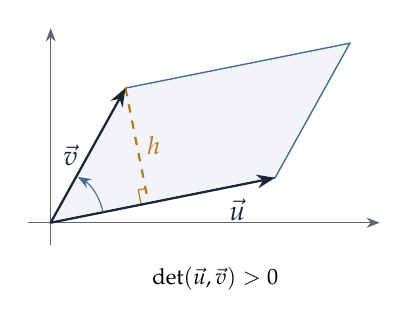
\begin{tikzpicture}[scale=0.95,>=Stealth]
  \draw[->,Gris] (-0.3,0)--(4.4,0); \draw[->,Gris] (0,-0.3)--(0,2.6);
  \fill[Fond,draw=BleuMoyen,line width=0.5pt] (0,0)--(3,0.6)--(4,2.4)--(1,1.8)--cycle;
  \draw[Ocre,dashed,line width=0.8pt] (1,1.8)--(1.3077,0.2615) node[midway,right,font=\small]{$h$};
  \draw[Ocre,line width=0.4pt] (1.2097,0.2419)--(1.1707,0.4380)--(1.2687,0.4576);
  \draw[->,thick,Ink] (0,0)--(3,0.6) node[pos=0.75,below right]{$\ve u$};
  \draw[->,thick,Ink] (0,0)--(1,1.8) node[midway,left]{$\ve v$};
  \draw[->,BleuMoyen] (0.7,0.14) arc (11:60:0.7);
  \node[font=\footnotesize\sffamily,align=center] at (2.2,-0.75) {$\det(\ve u,\ve v)>0$};
\end{tikzpicture}\hfill
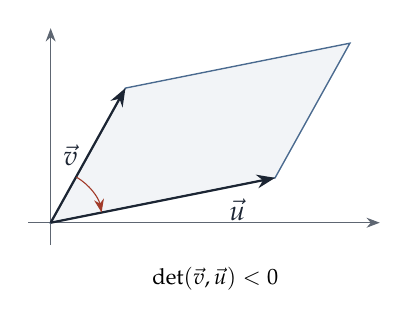
\begin{tikzpicture}[scale=0.95,>=Stealth]
  \draw[->,Gris] (-0.3,0)--(4.4,0); \draw[->,Gris] (0,-0.3)--(0,2.6);
  \fill[Fond,draw=BleuMoyen,line width=0.5pt] (0,0)--(3,0.6)--(4,2.4)--(1,1.8)--cycle;
  \draw[->,thick,Ink] (0,0)--(1,1.8) node[midway,left]{$\ve v$};
  \draw[->,thick,Ink] (0,0)--(3,0.6) node[pos=0.75,below right]{$\ve u$};
  \draw[->,Brique] (0.7*0.4903,0.7*0.8716) arc (60:11:0.7);
  \node[font=\footnotesize\sffamily] at (2.2,-0.75) {$\det(\ve v,\ve u)<0$};
\end{tikzpicture}\hfill
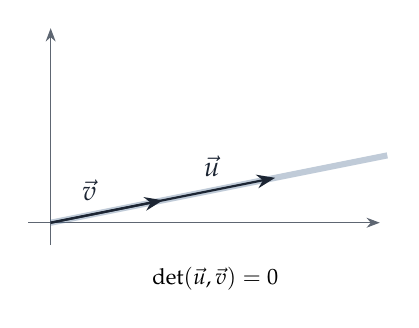
\begin{tikzpicture}[scale=0.95,>=Stealth]
  \draw[->,Gris] (-0.3,0)--(4.4,0); \draw[->,Gris] (0,-0.3)--(0,2.6);
  \draw[BleuMoyen,line width=2.2pt,opacity=0.35] (0,0)--(4.5,0.9);
  \draw[->,thick,Ink] (0,0)--(3,0.6) node[pos=0.8,above left]{$\ve u$};
  \draw[->,thick,Ink] (0,0)--(1.5,0.3) node[midway,above left]{$\ve v$};
  \node[font=\footnotesize\sffamily] at (2.2,-0.75) {$\det(\ve u,\ve v)=0$};
\end{tikzpicture}
\caption{Aire orientée. À gauche, $\ve u$ et $\ve v$ dans le sens direct ; au centre, les mêmes vecteurs dans l'ordre inverse ;
à droite, deux vecteurs colinéaires.}\label{fig:aire2}
\end{figure}

\begin{lecture}
\emph{À gauche} : le parallélogramme gris a pour base $\|\ve u\|$ et pour hauteur $h$, distance de l'extrémité de $\ve v$
à la droite portée par $\ve u$ (segment ocre, perpendiculaire à $\ve u$). Si $\theta$ est l'angle de $\ve u$ à $\ve v$, on a
$h=\|\ve v\|\,|\sin\theta|$, donc l'aire vaut $\|\ve u\|\,\|\ve v\|\,|\sin\theta|$ : c'est $|\det(\ve u,\ve v)|$. La flèche
indique qu'on tourne de $\ve u$ vers $\ve v$ dans le sens direct : le déterminant est positif.
\emph{Au centre} : même parallélogramme, donc même aire ; mais on tourne de $\ve v$ vers $\ve u$ dans le sens horaire, et le
signe change. C'est l'\emph{antisymétrie} : $\det(\ve v,\ve u)=-\det(\ve u,\ve v)$, propriété qui servira de définition à
l'étape 3.
\emph{À droite} : $\ve v$ est colinéaire à $\ve u$ ; le parallélogramme est « aplati » sur une droite, sa hauteur est nulle,
son aire aussi. C'est la raison géométrique du test de colinéarité.
\end{lecture}

\begin{proposition}\label{prop:aire}
Dans une base orthonormée directe, $\det(\ve u,\ve v)=\|\ve u\|\,\|\ve v\|\sin\theta$, où $\theta$ mesure l'angle
orienté $(\ve u,\ve v)$. Par conséquent :
\begin{enumerate}
\item $|\det(\ve u,\ve v)|$ est l'aire du parallélogramme construit sur $\ve u$ et $\ve v$ ;
\item $\det(\ve u,\ve v)>0$ si et seulement si l'on passe de $\ve u$ à $\ve v$ dans le sens direct ;
\item $\det(\ve u,\ve v)=0$ si et seulement si $\ve u$ et $\ve v$ sont colinéaires.
\end{enumerate}
\end{proposition}

\begin{proof}
On écrit $\ve u=\|\ve u\|(\cos\alpha,\sin\alpha)$ et $\ve v=\|\ve v\|(\cos\beta,\sin\beta)$.
\begin{itemize}
\item Calcul : $\det(\ve u,\ve v)=\|\ve u\|\|\ve v\|(\cos\alpha\sin\beta-\sin\alpha\cos\beta)=\|\ve u\|\|\ve v\|\sin(\beta-\alpha)$.
\item Aire : base fois hauteur, et la hauteur issue de l'extrémité de $\ve v$ vaut $\|\ve v\|\,|\sin(\beta-\alpha)|$.
\item Colinéarité : $\sin\theta=0$ exactement lorsque les deux vecteurs ont même direction.\qedhere
\end{itemize}
\end{proof}

\marge{Questionner}
\question{Pourquoi un parallélogramme « aplati » a-t-il une aire nulle ? Que dire des vecteurs qui le construisent ?}

\begin{reflexe}
Devant les mots « colinéaires », « parallèles », « alignés », on calcule un déterminant $2\times2$ : la réponse est
« oui » si et seulement s'il est nul. Le test ne demande aucune division et reste valable si une coordonnée est nulle.
\end{reflexe}

\marge{Ensemble}
\begin{exemple}[répondre à la question de départ]
$\dt{2&-3\\-4&6}=2\times6-(-3)\times(-4)=12-12=0$ : les vecteurs sont colinéaires. On vérifie ensuite que
$(-3,6)=-\frac32(2,-4)$, mais le déterminant a répondu sans qu'il faille deviner ce coefficient.
\end{exemple}

\begin{exemple}[avec un paramètre]
Pour quelles valeurs de $m$ les vecteurs $\ve u=(m,2)$ et $\ve v=(8,m)$ sont-ils colinéaires ?
\chercher
\etape{Reconnaître} « Colinéaires ? » se traduit par « déterminant nul ? ».
\etape{Calculer} $\det(\ve u,\ve v)=m^2-16=(m-4)(m+4)$.
\etape{Conclure} Colinéaires si et seulement si $m=4$ ou $m=-4$ ; on contrôle : pour $m=4$, $\ve v=(8,4)=2\ve u$.
\end{exemple}

\begin{astuce}
Avec un paramètre, on \emph{factorise} le déterminant avant de conclure : la condition « $=0$ » se lit alors
immédiatement, facteur par facteur. Ce réflexe sera la clé de l'étape 5.
\end{astuce}

\marge{Seul}
\begin{exo}{d2-param}{2}{colinéarité avec paramètre}
Pour quelles valeurs de $\lambda\in\R$ les vecteurs $(\lambda-1,3)$ et $(2,\lambda)$ sont-ils colinéaires ?
\end{exo}
\coupdepouce{écrire le déterminant des deux vecteurs, puis factoriser le polynôme du second degré obtenu.}

% ---------------------------------------------------------------------
\Etape{2}{8 min}{Le déterminant de trois vecteurs de l'espace}{calculer un déterminant $3\times3$ et l'interpréter.}

\pourquoi Revenons à la question initiale : trois vecteurs de $\R^3$ forment une base si et seulement s'ils ne sont
pas \emph{coplanaires}. Dans le plan, l'aire d'un parallélogramme détectait la colinéarité ; dans l'espace, c'est le
volume d'un parallélépipède qui détectera la coplanarité.

\rappel{produit mixte} En première année, on a défini $[\ve u,\ve v,\ve w]=(\ve u\wedge\ve v)\cdot\ve w$ ; il est nul si et
seulement si les vecteurs sont coplanaires, et sa valeur absolue est le volume du parallélépipède construit sur eux.

\marge{Expliquer}
\begin{definition}
Le déterminant de trois vecteurs de coordonnées $(x,y,z)$, $(x',y',z')$, $(x'',y'',z'')$ est
\begin{equation}\label{eq:det3}
\dt{x&x'&x''\\y&y'&y''\\z&z'&z''}
=x\dt{y'&y''\\z'&z''}-y\dt{x'&x''\\z'&z''}+z\dt{x'&x''\\y'&y''}.
\end{equation}
\end{definition}

On parcourt la première colonne ; chaque coefficient est multiplié par le déterminant $2\times2$ obtenu en \emph{rayant
sa ligne et sa colonne}, avec les signes $+,-,+$. En base orthonormée directe, ce nombre est exactement le produit
mixte : il est nul si et seulement si les trois vecteurs sont coplanaires, et sa valeur absolue est un volume.

\begin{figure}[H]
\centering
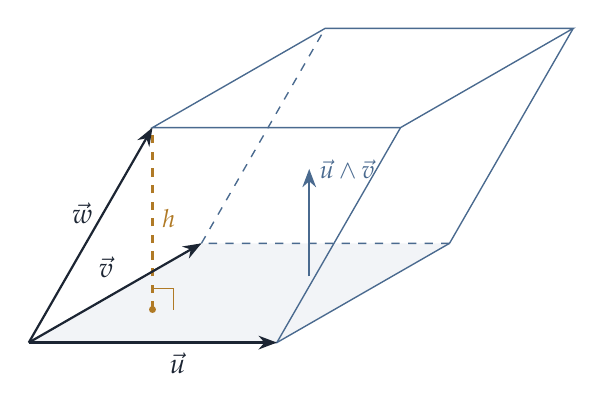
\begin{tikzpicture}[scale=1.05,>=Stealth,x={(1cm,0cm)},y={(0.62cm,0.5cm)},z={(0cm,1cm)}]
  \coordinate (O) at (0,0,0); \coordinate (U) at (3,0,0); \coordinate (V) at (0.6,2.4,0); \coordinate (W) at (1,0.8,2.2);
  \coordinate (UV) at (3.6,2.4,0); \coordinate (UW) at (4,0.8,2.2); \coordinate (VW) at (1.6,3.2,2.2); \coordinate (UVW) at (4.6,3.2,2.2);
  % base
  \fill[Fond] (O)--(U)--(UV)--(V)--cycle;
  \draw[BleuMoyen,line width=0.5pt] (O)--(U)--(UV);
  \draw[BleuMoyen,line width=0.5pt,dashed] (UV)--(V)--(O);
  % arêtes latérales et face supérieure
  \draw[BleuMoyen,line width=0.5pt] (U)--(UW) (UV)--(UVW);
  \draw[BleuMoyen,line width=0.5pt,dashed] (V)--(VW);
  \draw[BleuMoyen,line width=0.5pt] (W)--(UW)--(UVW)--(VW)--cycle;
  % hauteur
  \coordinate (Wp) at (1,0.8,0);
  \draw[Ocre,dashed,line width=0.9pt] (Wp)--(W);
  \node[Ocre,font=\small,right] at (1,0.8,1.1) {$h$};
  \draw[Ocre,line width=0.4pt] (1.25,0.8,0)--(1.25,0.8,0.25)--(1,0.8,0.25);
  \fill[Ocre] (Wp) circle (1.2pt);
  % normale
  \draw[->,thick,BleuMoyen] (2.4,1.6,0)--(2.4,1.6,1.3) node[right,font=\small]{$\ve u\wedge\ve v$};
  % vecteurs
  \draw[->,thick,Ink] (O)--(U) node[pos=0.6,below]{$\ve u$};
  \draw[->,thick,Ink] (O)--(V) node[pos=0.55,above left]{$\ve v$};
  \draw[->,thick,Ink] (O)--(W) node[pos=0.6,left]{$\ve w$};
\end{tikzpicture}\hspace{0.8cm}
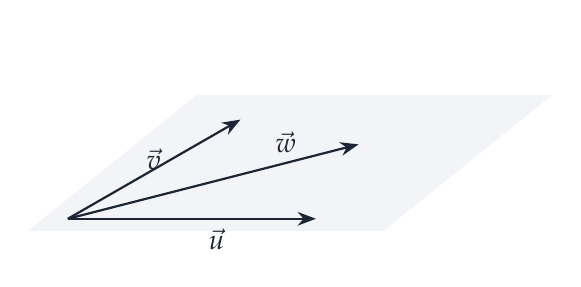
\begin{tikzpicture}[scale=1.05,>=Stealth,x={(1cm,0cm)},y={(0.62cm,0.5cm)},z={(0cm,1cm)}]
  \fill[Fond] (-0.3,-0.3,0)--(4,-0.3,0)--(4,3,0)--(-0.3,3,0)--cycle;
  \draw[->,thick,Ink] (0,0,0)--(3,0,0) node[pos=0.6,below]{$\ve u$};
  \draw[->,thick,Ink] (0,0,0)--(0.6,2.4,0) node[pos=0.6,left]{$\ve v$};
  \draw[->,thick,Ink] (0,0,0)--(2.4,1.8,0) node[pos=0.75,above]{$\ve w$};
  \node at (0,0,2.2) {};
\end{tikzpicture}
\caption{À gauche, le parallélépipède construit sur $\ve u,\ve v,\ve w$, de base grisée (aire $\|\ve u\wedge\ve v\|$) et de hauteur $h$ ; à droite, trois vecteurs coplanaires : $\ve w$ est dans le plan de $\ve u$ et $\ve v$.}\label{fig:volume}
\end{figure}

\begin{lecture}
\emph{À gauche} : la base du parallélépipède (en gris) est le parallélogramme construit sur $\ve u$ et $\ve v$ ; son aire
est $\|\ve u\wedge\ve v\|$, et le vecteur $\ve u\wedge\ve v$ (en bleu) lui est orthogonal. La hauteur $h$ (en ocre) est la
distance de l'extrémité de $\ve w$ au plan de la base : c'est la longueur de la projection de $\ve w$ sur la direction de
$\ve u\wedge\ve v$, soit $h=\dfrac{|\ve w\cdot(\ve u\wedge\ve v)|}{\|\ve u\wedge\ve v\|}$. Le volume vaut donc
\[\text{aire de la base}\times h=\|\ve u\wedge\ve v\|\times\frac{|(\ve u\wedge\ve v)\cdot\ve w|}{\|\ve u\wedge\ve v\|}
=|(\ve u\wedge\ve v)\cdot\ve w|=|\det(\ve u,\ve v,\ve w)|.\]
C'est exactement le passage de l'aire (étape 1) au volume : on multiplie par une hauteur de plus. Le signe du
déterminant indique si $\ve w$ est du même côté de la base que $\ve u\wedge\ve v$ (base directe) ou de l'autre côté.
\emph{À droite} : si $\ve w$ est dans le plan de $\ve u$ et $\ve v$, le parallélépipède est aplati, sa hauteur et son volume
sont nuls. D'où le critère : \emph{trois vecteurs forment une base de $\R^3$ si et seulement si leur déterminant est non nul}.
\end{lecture}

\marge{Ensemble}
\begin{exemple}
$\dt{1&2&0\\0&1&3\\2&0&1}=1\cdot\dt{1&3\\0&1}-0\cdot\dt{2&0\\0&1}+2\cdot\dt{2&0\\1&3}=1-0+12=13$. Les vecteurs ne sont
pas coplanaires : ils forment une base de $\R^3$.
\end{exemple}

Dans ce calcul, le zéro de la première colonne a supprimé un terme sans effort. Cette observation, généralisée à
l'étape 5, est à l'origine de toutes les techniques de calcul : \emph{plus il y a de zéros, plus le calcul est court}.

\begin{attention}
Pour un déterminant $3\times3$, on peut aussi utiliser la règle de Sarrus,
\[\dt{a&b&c\\d&e&f\\g&h&i}=aei+bfg+cdh-ceg-afh-bdi.\]
Elle est propre à la dimension~3 : en taille~4, elle ne
produirait que $8$ des $24$ termes, et le résultat serait faux.
\end{attention}

\marge{Seul}
\begin{exo}{d3-base}{2}{coplanarité, base de $\R^3$}
Les vecteurs $(1,1,0)$, $(0,1,1)$ et $(1,0,1)$ forment-ils une base de $\R^3$ ? Calculer le volume du parallélépipède
construit sur $(1,0,0)$, $(1,2,0)$ et $(1,1,3)$.
\end{exo}
\coupdepouce{écrire les trois vecteurs en colonnes ; développer selon une colonne qui contient un zéro. Le second déterminant est triangulaire.}

% ---------------------------------------------------------------------
\Etape{3}{20 min}{Le déterminant d'une matrice carrée}{connaître la définition générale et calculer par
opérations élémentaires.}

\pourquoi En dimension $4$ ou plus, aucune formule explicite n'est utilisable à la main. Il faut des \emph{règles} qui
permettent de simplifier un déterminant avant de le calculer. Ces règles se lisent sur les cas déjà connus.

\marge{Questionner}
\question{Sur la formule $\dt{a&b\\c&d}=ad-bc$ : que devient le déterminant si l'on multiplie la première colonne par
$2$ ? Si l'on échange les deux colonnes ? Que vaut-il pour la matrice identité ?}
(Il est multiplié par $2$ ; il change de signe ; il vaut $1$.)

\marge{Expliquer}
Ces trois observations, vraies aussi en taille $3$, deviennent la \emph{définition} en taille $n$.

\begin{theoreme}[admis]\label{thm:def}
Il existe une unique application $\det:\Mn{\K}\to\K$ telle que :
\begin{enumerate}
\item $\det$ est linéaire par rapport à chacune des colonnes, les autres étant fixées ;
\item échanger deux colonnes change le déterminant en son opposé ;
\item $\det(I_n)=1$.
\end{enumerate}
\end{theoreme}

\begin{votrecours}
En classe, le déterminant a été \emph{défini par récurrence} : $\dt{a&b\\c&d}=ad-bc$, puis, en taille $n\geq3$, par le
développement selon une ligne (ou une colonne) fixée,
\[\det A=\sum_{j=1}^n(-1)^{i+j}a_{i,j}\Delta_{i,j},\]
où $\Delta_{i,j}$ est le déterminant extrait de $A$ en supprimant la ligne $i$ et la colonne $j$ (le \emph{mineur} de
$a_{i,j}$). Les deux présentations définissent \emph{la même} application : le déterminant défini par récurrence vérifie
les trois propriétés du théorème, et ces propriétés le caractérisent. Le programme officiel part de la caractérisation
et admet le développement (étape 5) ; votre cours part du développement. Dans un exercice, on utilise librement l'un ou
l'autre point de vue : les propriétés pour transformer, le développement pour conclure.
\end{votrecours}

« Linéaire par rapport à une colonne » signifie qu'on peut \emph{sortir un facteur} d'une colonne, ou \emph{découper}
une colonne en somme :
\[\det(\lambda C_1,C_2,\dots,C_n)=\lambda\det(C_1,C_2,\dots,C_n).\]

\begin{proposition}\label{prop:egales}
\begin{enumerate}
\item Si $A$ a une colonne nulle ou deux colonnes égales, alors $\det A=0$.
\item Pour $\lambda\in\K$, $\det(\lambda A)=\lambda^n\det A$.
\end{enumerate}
\end{proposition}

\begin{proof}
\begin{itemize}
\item Une colonne nulle s'écrit $0\cdot C$ : on sort le facteur $0$.
\item Si deux colonnes sont égales, les échanger ne modifie pas $A$ mais change le signe : $\det A=-\det A$, donc $\det A=0$.
\item $\lambda A$ s'obtient en multipliant chacune des $n$ colonnes par $\lambda$ : il sort $n$ facteurs.\qedhere
\end{itemize}
\end{proof}

\begin{attention}
Le déterminant n'est pas linéaire. Pour $A\in\mathcal M_3(\R)$ avec $\det A=2$ : $\det(2A)=2^3\times2=16$, alors que
$\det A+\det A=4$. En général $\det(A+B)\neq\det A+\det B$, et $\det(\lambda A)=\lambda^n\det A$, non $\lambda\det A$.
\end{attention}

\rappel{opérations élémentaires} Ce sont celles du pivot de Gauss : l'échange $C_i\leftrightarrow C_j$, la dilatation
$C_i\leftarrow\lambda C_i$ ($\lambda\neq0$) et la transvection $C_i\leftarrow C_i+\lambda C_j$ ($j\neq i$) ; on les note
de même sur les lignes.

\marge{Expliquer}
\begin{proposition}\label{prop:op}
\begin{enumerate}
\item Un échange $C_i\leftrightarrow C_j$ change le déterminant en son opposé.
\item Une dilatation $C_i\leftarrow\lambda C_i$ multiplie le déterminant par $\lambda$.
\item Une transvection $C_i\leftarrow C_i+\lambda C_j$ \emph{ne change pas} le déterminant.
\end{enumerate}
\end{proposition}

\begin{proof}
Les deux premiers points traduisent la définition. Pour le troisième, on découpe la colonne $i$ :
$\det(\dots,C_i+\lambda C_j,\dots)=\det(\dots,C_i,\dots)+\lambda\det(\dots,C_j,\dots,C_j,\dots)$, et le dernier
déterminant a deux colonnes égales.
\end{proof}

\begin{figure}[H]
\centering
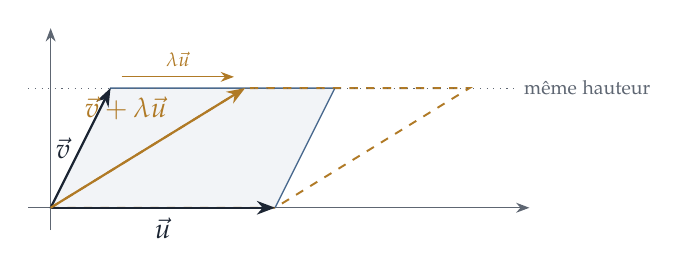
\begin{tikzpicture}[scale=0.95,>=Stealth]
  \draw[->,Gris] (-0.3,0)--(6.4,0); \draw[->,Gris] (0,-0.3)--(0,2.4);
  \fill[Fond,draw=BleuMoyen,line width=0.5pt] (0,0)--(3,0)--(3.8,1.6)--(0.8,1.6)--cycle;
  \draw[Ocre,line width=0.7pt,dashed] (0,0)--(3,0)--(5.6,1.6)--(2.6,1.6)--cycle;
  \draw[Gris,dotted] (-0.3,1.6)--(6.2,1.6) node[right,font=\scriptsize]{même hauteur};
  \draw[->,thick,Ink] (0,0)--(3,0) node[midway,below]{$\ve u$};
  \draw[->,thick,Ink] (0,0)--(0.8,1.6) node[midway,left]{$\ve v$};
  \draw[->,thick,Ocre] (0,0)--(2.6,1.6) node[pos=0.65,above left]{$\ve v+\lambda\ve u$};
  \draw[->,Ocre] (0.95,1.75)--(2.45,1.75) node[midway,above,font=\scriptsize]{$\lambda\ve u$};
\end{tikzpicture}
\caption{Une transvection $\ve v\leftarrow\ve v+\lambda\ve u$ fait glisser le parallélogramme sans changer son aire.}\label{fig:transvection}
\end{figure}

\begin{lecture}
Le parallélogramme gris est construit sur $\ve u$ et $\ve v$, le parallélogramme ocre sur $\ve u$ et $\ve v+\lambda\ve u$. Le
côté supérieur a simplement glissé de $\lambda\ve u$, parallèlement à la base : la base $\|\ve u\|$ et la hauteur (pointillés)
sont les mêmes, donc l'aire est la même. Voilà pourquoi une transvection ne change pas le déterminant. À l'inverse, une
dilatation $\ve v\leftarrow\lambda\ve v$ multiplie la hauteur, donc l'aire, par $|\lambda|$ ; un échange ne change pas l'aire
mais inverse le sens de rotation, donc le signe.
\end{lecture}

On admet aussi que $\det(A^T)=\det A$ : transposer échange lignes et colonnes, donc \emph{les mêmes règles valent pour
les lignes}. On choisit, à chaque étape, l'opération qui crée le plus vite des zéros.

\begin{enpratique}
Chaque opération a son usage. La \emph{transvection} crée des zéros sans rien changer : c'est l'outil principal.
La \emph{dilatation} sert à l'envers, pour sortir un facteur commun à toute une ligne ou une colonne. L'\emph{échange}
sert à amener un coefficient non nul (idéalement $1$) en position de pivot.
\end{enpratique}

\marge{Ensemble}
\begin{exemple}[l'erreur la plus fréquente]
On sait que $\dt{1&2\\3&4}=-2$. Après « $C_2\leftarrow2C_2-C_1$ », on obtient $\dt{1&3\\3&5}=-4$.
\chercher
Le déterminant a été multiplié par $2$ : l'opération est une dilatation de $C_2$ par $2$ suivie d'une transvection.
\end{exemple}

\begin{attention}
Dans une transvection, la colonne modifiée doit garder le coefficient $1$. Les opérations s'effectuent l'une après
l'autre, chacune sur la matrice obtenue à l'étape précédente.
\end{attention}

\marge{Expliquer}
\begin{theoreme}\label{thm:tri}
Le déterminant d'une matrice triangulaire est le produit de ses coefficients diagonaux.
\end{theoreme}

\begin{proof}
Soit $T$ triangulaire supérieure, de diagonale $t_{1,1},\dots,t_{n,n}$.
\begin{itemize}
\item Si les $t_{k,k}$ sont non nuls : on sort $t_{1,1}$ de la première colonne, qui devient $e_1$ ; les transvections
      $C_j\leftarrow C_j-t_{1,j}C_1$ annulent le reste de la première ligne. On recommence avec la deuxième colonne, et
      l'on aboutit à $t_{1,1}\cdots t_{n,n}\det I_n$.
\item Si $t_{k,k}=0$ : les $k$ premières colonnes sont dans $\vect(e_1,\dots,e_{k-1})$, de dimension $k-1$. Elles sont
      liées, et des transvections rendent l'une d'elles nulle : le déterminant est nul.\qedhere
\end{itemize}
\end{proof}

\begin{votrecours}
Le cours démontre ce théorème par récurrence, en développant selon la dernière ligne. Pour $T$ triangulaire supérieure,
cette ligne vaut $(0,\dots,0,t_{n,n})$, donc $\det T=(-1)^{n+n}t_{n,n}\Delta_{n,n}=t_{n,n}\Delta_{n,n}$ ; or $\Delta_{n,n}$
est le déterminant de la matrice triangulaire d'ordre $n-1$ de diagonale $t_{1,1},\dots,t_{n-1,n-1}$, égal par hypothèse
de récurrence à $t_{1,1}\cdots t_{n-1,n-1}$. Cette preuve est plus courte que la précédente, mais elle s'appuie sur le
développement, que le livre n'introduit qu'à l'étape 5.
\end{votrecours}

Ce théorème donne enfin une méthode de calcul générale.

\begin{methode}{Calcul par le pivot de Gauss}\label{meth:pivot}
\begin{enumerate}
\item Choisir un pivot non nul (un $1$ si possible), au besoin par un échange, en notant le changement de signe.
\item Annuler les coefficients situés sous le pivot par des transvections.
\item Recommencer avec la colonne suivante jusqu'à obtenir une matrice triangulaire.
\item Faire le produit des coefficients diagonaux, corrigé des signes et des facteurs sortis.
\end{enumerate}
\end{methode}

\marge{Ensemble}
\begin{exemple}
Calculer le déterminant
\[D=\dt{1&2&1&0\\2&5&3&1\\1&3&3&2\\0&1&2&4}.\]
\chercher
Avec $L_2\leftarrow L_2-2L_1$ et $L_3\leftarrow L_3-L_1$, puis $L_3\leftarrow L_3-L_2$, $L_4\leftarrow L_4-L_2$ et enfin
$L_4\leftarrow L_4-L_3$ :
\[D=\dt{1&2&1&0\\0&1&1&1\\0&1&2&2\\0&1&2&4}=\dt{1&2&1&0\\0&1&1&1\\0&0&1&1\\0&0&0&2}=2.\]
Seules des transvections ont servi : aucune correction n'est nécessaire.
\end{exemple}

\marge{Seul}
\begin{exo}{m-pivot}{2}{triangulation par le pivot}
Calculer par opérations élémentaires :
\[D_1=\dt{1&2&3\\4&5&6\\7&8&10},\qquad D_2=\dt{0&2&1\\3&0&1\\1&1&0},\qquad
D_3=\dt{1&1&1&1\\1&2&2&2\\1&2&3&3\\1&2&3&4}.\]
\end{exo}

\coupdepouce{pour $D_1$, utiliser le $1$ en haut à gauche comme pivot ; pour $D_3$, retrancher chaque ligne à la suivante, en commençant par le bas.}

En séance, on traite $D_1$ et $D_3$ ; $D_2$, dont le pivot est nul, est laissé en travail personnel.

\pointarret{la définition et le calcul sont acquis. Reprise à l'étape 4, en refaisant d'abord $D_1$ au tableau.}

% ---------------------------------------------------------------------
\Etape{4}{15 min}{Déterminant, inversibilité et bases}{répondre à « est-ce une base ? » et « est-ce inversible ? » par
un seul calcul.}

\pourquoi On sait maintenant calculer un déterminant. Il reste à démontrer qu'il répond à la question posée au début
du chapitre, en dimension quelconque.

\rappel{inversibilité} Une matrice $A$ de taille $n$ est inversible si et seulement si $\rg A=n$, si et seulement si ses
colonnes forment une base de $\K^n$, si et seulement si le système $AX=Y$ a une unique solution pour tout $Y$.

\marge{Expliquer}
\begin{theoreme}\label{thm:fond}
Soient $A,B\in\Mn{\K}$.
\begin{enumerate}
\item $A$ est inversible si et seulement si $\det A\neq0$ ; autrement dit, $\det A=0$ si et seulement si les colonnes
      de $A$ sont liées.
\item $\det(AB)=\det A\,\det B$ \quad (admis).
\item Si $A$ est inversible, $\det(A^{-1})=\dfrac1{\det A}$.
\end{enumerate}
\end{theoreme}

\begin{proof}[Démonstration des points 1 et 3]
\begin{itemize}
\item Si les colonnes sont liées, par exemple $C_i=\sum_{j\neq i}\lambda_jC_j$, la transvection
      $C_i\leftarrow C_i-\sum_{j\neq i}\lambda_jC_j$ rend la colonne $i$ nulle sans changer le déterminant : $\det A=0$.
\item Si $A$ est inversible, $\det A\cdot\det A^{-1}=\det(AA^{-1})=\det I_n=1$ : donc $\det A\neq0$, et l'on obtient
      le point 3.\qedhere
\end{itemize}
\end{proof}

\paragraph{Inverse d'une matrice $2\times2$} Si $ad-bc\neq0$,
\[\begin{pmatrix}a&b\\c&d\end{pmatrix}^{-1}=\frac1{ad-bc}\begin{pmatrix}d&-b\\-c&a\end{pmatrix} :\]
on échange les coefficients diagonaux, on change le signe des deux autres et l'on divise par le déterminant. On le
vérifie en effectuant le produit : $\begin{pmatrix}a&b\\c&d\end{pmatrix}\begin{pmatrix}d&-b\\-c&a\end{pmatrix}
=\begin{pmatrix}ad-bc&0\\0&ad-bc\end{pmatrix}=(ad-bc)I_2$.

\begin{horsprogramme}\phantomsection\label{hp:comatrice}
\textbf{Comatrice.} Le \emph{cofacteur} de $a_{i,j}$ est $(-1)^{i+j}\Delta_{i,j}$, où $\Delta_{i,j}$ est le déterminant
obtenu en supprimant la ligne $i$ et la colonne $j$ ; la \emph{comatrice} $\mathrm{com}(A)$ est la matrice des cofacteurs. Pour
toute matrice carrée $A$,
\[A\,\mathrm{com}(A)^T=\mathrm{com}(A)^T A=\det(A)\,I_n,\]
donc, si $\det A\neq0$, $A^{-1}=\dfrac1{\det A}\,\mathrm{com}(A)^T$.
\emph{Pourquoi.} Le coefficient $(i,i)$ de $A\,\mathrm{com}(A)^T$ vaut $\sum_ja_{i,j}(-1)^{i+j}\Delta_{i,j}$ : c'est le
développement de $\det A$ selon la ligne $i$. Pour $k\neq i$, le coefficient $(k,i)$ vaut
$\sum_ja_{k,j}(-1)^{i+j}\Delta_{i,j}$ : c'est le développement, selon la ligne $i$, du déterminant de la matrice obtenue
en remplaçant la ligne $i$ de $A$ par sa ligne $k$ ; cette matrice a deux lignes égales, d'où $0$.
En taille $2$, $\mathrm{com}(A)=\begin{pmatrix}d&-c\\-b&a\end{pmatrix}$ et l'on retrouve la formule ci-dessus. En
pratique, la formule ne sert qu'en taille $2$ ou $3$, ou pour des questions théoriques (exercice~\ref{e:hp-com}) ; au-delà,
le pivot de Gauss est bien plus rapide.
\end{horsprogramme}

\begin{enpratique}
Les règles du point 2 et 3, avec $\det(\lambda A)=\lambda^n\det A$ et $\det(A^T)=\det A$, permettent de calculer le
déterminant d'une expression \emph{sans connaître les matrices}. Par exemple, deux matrices semblables ont même
déterminant : $\det(P^{-1}AP)=\frac1{\det P}\det A\det P=\det A$.
\end{enpratique}

\marge{Ensemble}
\begin{exemple}
Si $A,B\in\mathcal M_3(\R)$ vérifient $\det A=3$ et $\det B=-2$, calculer $\det(A^2B^T)$ et $\det(2A^{-1}B)$.
\chercher
$\det(A^2B^T)=3^2\times(-2)=-18$ ; $\det(2A^{-1}B)=2^3\times\frac13\times(-2)=-\frac{16}3$ : on n'oublie pas le facteur
$2^3$.
\end{exemple}

\marge{Expliquer}
Pour des vecteurs d'un espace $E$ de dimension $n$, on se ramène à une matrice : le \emph{déterminant d'une famille}
$(u_1,\dots,u_n)$ dans une base $\mathcal B$ est celui de la matrice dont la colonne $j$ contient les coordonnées de
$u_j$. De même, le \emph{déterminant d'un endomorphisme} $f$ est celui de sa matrice dans une base ; il ne dépend pas
de la base choisie, puisque deux matrices de $f$ sont semblables.

\begin{figure}[H]
\centering
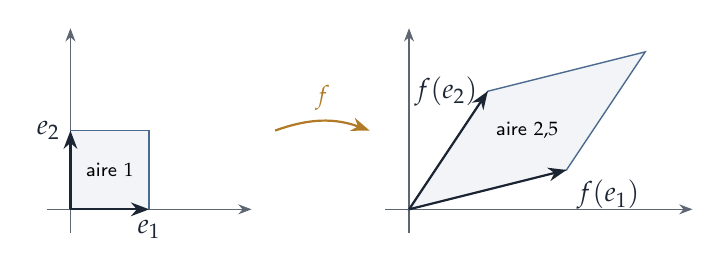
\begin{tikzpicture}[scale=1.0,>=Stealth]
  \draw[->,Gris] (-0.3,0)--(2.3,0); \draw[->,Gris] (0,-0.3)--(0,2.3);
  \fill[Fond,draw=BleuMoyen,line width=0.5pt] (0,0)--(1,0)--(1,1)--(0,1)--cycle;
  \draw[->,thick,Ink] (0,0)--(1,0) node[below]{$e_1$};
  \draw[->,thick,Ink] (0,0)--(0,1) node[left]{$e_2$};
  \node[font=\scriptsize\sffamily] at (0.5,0.5) {aire $1$};
  \draw[->,Ocre,thick] (2.6,1.0) to[bend left=20] node[above,font=\small]{$f$} (3.8,1.0);
  \begin{scope}[xshift=4.3cm]
  \draw[->,Gris] (-0.3,0)--(3.6,0); \draw[->,Gris] (0,-0.3)--(0,2.3);
  \fill[Fond,draw=BleuMoyen,line width=0.5pt] (0,0)--(2,0.5)--(3,2)--(1,1.5)--cycle;
  \draw[->,thick,Ink] (0,0)--(2,0.5) node[below right]{$f(e_1)$};
  \draw[->,thick,Ink] (0,0)--(1,1.5) node[left]{$f(e_2)$};
  \node[font=\scriptsize\sffamily] at (1.5,1.0) {aire $2{,}5$};
  \end{scope}
\end{tikzpicture}
\caption{L'endomorphisme $f$ de matrice $\begin{pmatrix}2&1\\0{,}5&1{,}5\end{pmatrix}$ transforme le carré unité en un
parallélogramme d'aire $|\det f|=2{,}5$.}\label{fig:endo}
\end{figure}

\begin{lecture}
Le carré construit sur $(e_1,e_2)$ a pour aire $1$. Son image est le parallélogramme construit sur $f(e_1)$ et $f(e_2)$,
c'est-à-dire sur les \emph{colonnes} de la matrice de $f$ ; son aire est donc $|\det f|=|2\times1{,}5-1\times0{,}5|=2{,}5$.
Plus généralement, pour deux vecteurs quelconques, $\det\big(f(\ve u),f(\ve v)\big)=\det f\cdot\det(\ve u,\ve v)$ par
multiplicativité : $f$ multiplie toutes les aires par $|\det f|$. Si $\det f=0$, le carré est écrasé sur une droite, et
deux vecteurs distincts ont la même image : $f$ n'est pas injective. Le théorème suivant énonce ce fait en toute dimension.
\end{lecture}

\begin{theoreme}\label{thm:base}
Dans un espace de dimension $n$ :
\begin{enumerate}
\item $n$ vecteurs forment une base si et seulement si leur déterminant dans une base est non nul ;
\item un endomorphisme $f$ est bijectif si et seulement si $\det f\neq0$.
\end{enumerate}
\end{theoreme}

\begin{reflexe}
« Est-ce une base ? » : on compte d'abord les vecteurs. S'il y en a exactement $n=\dim E$, on calcule leur déterminant
dans une base simple ; sinon, la question du déterminant n'a pas de sens.
\end{reflexe}

\marge{Ensemble}
\begin{exemple}[une famille de polynômes]
$\big(1,\ X-1,\ (X-1)^2\big)$ est-elle une base de $\R_2[X]$ ?
\chercher
Trois vecteurs dans un espace de dimension $3$. Dans la base $(1,X,X^2)$, leurs coordonnées sont $(1,0,0)$,
$(-1,1,0)$ et $(1,-2,1)$ :
$\dt{1&-1&1\\0&1&-2\\0&0&1}=1\neq0$. C'est une base.
\end{exemple}

\begin{astuce}
Pour un endomorphisme, on choisit la base dans laquelle la matrice est la plus simple. Pour $f:P\mapsto XP'+P$ sur
$\R_3[X]$, on a $f(X^k)=(k+1)X^k$ : dans la base canonique, la matrice est $\mathrm{diag}(1,2,3,4)$, donc $\det f=24$ et
$f$ est bijectif, sans aucun calcul de déterminant.
\end{astuce}

\marge{Seul}
\begin{exo}{m-lambda}{1}{$\det(\lambda A)$, $\det(A^T)$, $\det(AB)$}
Soient $A,B\in\mathcal M_4(\R)$ avec $\det A=-1$ et $\det B=5$. Calculer $\det(2A)$, $\det(-B)$, $\det(A^3)$,
$\det(AB^TA^{-1})$ et $\det(3A^{-1}B^2)$.
\end{exo}
\coupdepouce{ici $n=4$ ; ne jamais chercher les matrices, seulement appliquer $\det(AB)=\det A\det B$ et $\det(\lambda A)=\lambda^4\det A$.}

% ---------------------------------------------------------------------
\Etape{5}{15 min}{Calculer avec un paramètre}{développer selon une ligne, exploiter une somme constante, factoriser.}

\pourquoi La plupart des exercices posent la question « pour quelles valeurs de $m$\dots ? ». Il faut alors une forme
\emph{factorisée} du déterminant. Un calcul aveugle produit un polynôme développé qu'on ne sait plus factoriser ; on
apprend ici à garder les facteurs au fil du calcul.

\marge{Expliquer}
\paragraph{Développer selon une ligne} La formule~\eqref{eq:det3} de l'étape 2 développait selon la première colonne.
Elle se généralise à toute ligne et toute colonne. Notons $\Delta_{i,j}$ le déterminant obtenu en supprimant la ligne $i$
et la colonne $j$ de $A$.

\begin{theoreme}[admis]
Pour toute colonne $j$ et toute ligne $i$ :
\begin{align*}
\det A&=\sum_{i=1}^n(-1)^{i+j}a_{i,j}\Delta_{i,j} &&\text{(développement selon la colonne $j$)},\\
\det A&=\sum_{j=1}^n(-1)^{i+j}a_{i,j}\Delta_{i,j} &&\text{(développement selon la ligne $i$)}.
\end{align*}
\end{theoreme}

Les signes forment un damier commençant par $+$ en haut à gauche. Le développement n'a d'intérêt que selon une ligne
riche en zéros.

\marge{Ensemble}
\begin{exemple}
Dans $D=\dt{1&0&2&0\\3&0&1&4\\0&2&0&0\\1&0&1&1}$, la troisième ligne ne contient que le $2$ en position $(3,2)$, de signe
$(-1)^{3+2}=-1$. Donc $D=-2\dt{1&2&0\\3&1&4\\1&1&1}=-2\times(-1)=2$.
\end{exemple}

\marge{Questionner}
\paragraph{Exploiter une somme constante}
\question{Dans $D(x)=\dt{x&1&1\\1&x&1\\1&1&x}$, que remarque-t-on en additionnant les coefficients de chaque ligne ?}

\marge{Ensemble}
\begin{exemple}[cas simple]
Chaque ligne a pour somme $x+2$. L'opération $C_1\leftarrow C_1+C_2+C_3$ ne change pas le déterminant (c'est une
transvection, répétée) et remplit la première colonne de $x+2$, que l'on sort :
\[D(x)=(x+2)\dt{1&1&1\\1&x&1\\1&1&x}\underset{\substack{L_2\leftarrow L_2-L_1\\L_3\leftarrow L_3-L_1}}{=}(x+2)\dt{1&1&1\\0&x-1&0\\0&0&x-1}
=(x+2)(x-1)^2.\]
La forme factorisée donne aussitôt les valeurs qui annulent $D$ : $x=-2$ et $x=1$.
\end{exemple}

Pourquoi cela a-t-il marché ? Parce que la \emph{somme} des colonnes avait tous ses coefficients égaux : un facteur
commun est apparu, et la colonne de $1$ restante a permis de créer des zéros par simples soustractions de lignes. La
structure ne dépend pas de la taille, d'où la méthode et sa généralisation.

\begin{methode}{Somme constante sur les lignes}\label{meth:somme}
\begin{enumerate}
\item Vérifier que toutes les lignes ont la même somme $s$.
\item Effectuer $C_1\leftarrow C_1+C_2+\dots+C_n$, puis sortir $s$ de la première colonne.
\item Retrancher la première ligne aux autres : la première colonne n'a plus qu'un coefficient non nul.
\end{enumerate}
Même démarche, en échangeant les rôles, si ce sont les colonnes qui ont une somme constante.
\end{methode}

\begin{proposition}\label{prop:ab}
Le déterminant d'ordre $n$ dont les coefficients diagonaux valent $a$ et les autres $b$ est
$D_n(a,b)=\big(a+(n-1)b\big)(a-b)^{n-1}$.
\end{proposition}

\begin{proof}
Chaque ligne a pour somme $a+(n-1)b$. Après la méthode~\ref{meth:somme}, la ligne $L_i-L_1$ ($i\geq2$) vaut $a-b$ en
colonne $i$ et $0$ ailleurs : la matrice est triangulaire de diagonale $(1,a-b,\dots,a-b)$.
\end{proof}

\begin{enpratique}
Ce résultat intervient chaque fois qu'une matrice s'écrit $aI_n+b(J-I_n)$, où $J$ ne contient que des $1$, et dans les
questions « ces vecteurs forment-ils une base ? » où le paramètre est placé symétriquement, comme dans l'exercice
ci-dessous.
\end{enpratique}

\paragraph{Faire apparaître des différences}
Lorsque la somme n'est pas constante, on cherche à faire apparaître des facteurs du type $b-a$.

\marge{Ensemble}
\begin{exemple}
Pour $V=\dt{1&1&1\\a&b&c\\a^2&b^2&c^2}$, les opérations $C_2\leftarrow C_2-C_1$ et $C_3\leftarrow C_3-C_1$, puis un
développement selon la première ligne, donnent
\[V=\dt{b-a&c-a\\b^2-a^2&c^2-a^2}=(b-a)(c-a)\dt{1&1\\b+a&c+a}=(b-a)(c-a)(c-b),\]
en sortant $b-a$ et $c-a$ des colonnes. Ainsi $V\neq0$ si et seulement si $a$, $b$, $c$ sont distincts.
\end{exemple}

\begin{plusloin}
Ce déterminant est le premier cas du \emph{déterminant de Vandermonde}, dont la version générale, très utile pour les
problèmes d'interpolation, est démontrée au chapitre~\ref{sec:approf}.
\end{plusloin}

\begin{strategie}
Devant un déterminant à paramètre : (1) une somme constante ? (2) des lignes qui diffèrent d'un facteur commun ?
(3) une ligne riche en zéros, après quelques transvections ? On ne développe une expression complète qu'en dernier
recours, et l'on garde les facteurs au fil du calcul.
\end{strategie}

\marge{Seul}
\begin{exo}{t-base-m}{3}{paramètre et base}
Pour quelles valeurs de $m\in\R$ les vecteurs $\ve u=(1,1,m)$, $\ve v=(1,m,1)$ et $\ve w=(m,1,1)$ forment-ils une base
de $\R^3$ ?
\end{exo}
\coupdepouce{calculer la somme de chaque ligne de la matrice des trois vecteurs.}

% ---------------------------------------------------------------------
\subsection*{Bilan des déterminants}
\addcontentsline{toc}{subsection}{Bilan des déterminants {\color{Gris}(5 min)}}

\marge{Questionner}
On vérifie oralement, en cinq minutes, les acquis essentiels.
\begin{enumerate}
\item Comment savoir si trois vecteurs de $\R^3$ forment une base ? \hfill{\small\color{Gris}(déterminant non nul)}
\item Quelle opération ne change pas un déterminant ? Laquelle change son signe ? \hfill{\small\color{Gris}(transvection ; échange)}
\item Que vaut $\det(-A)$ pour $A\in\mathcal M_3(\R)$ ? \hfill{\small\color{Gris}($-\det A$)}
\item Pourquoi viser une forme factorisée ? \hfill{\small\color{Gris}(pour lire les valeurs qui l'annulent)}
\end{enumerate}
Si une réponse hésite, on reprendra l'étape correspondante au début de la séance 2.

\pointarret{fin du chapitre sur les déterminants. On peut arrêter ici une séance d'une heure et quart, ou enchaîner sur le chapitre 2.}

\begin{essentiel}\label{ess:1}
\begin{itemize}
\item $\det$ est linéaire par rapport à chaque colonne, change de signe par échange de deux colonnes, vaut $1$ en $I_n$.
\item Transvection : inchangé ; échange : $\times(-1)$ ; dilatation : $\times\lambda$. Mêmes règles sur les lignes.
\item Matrice triangulaire : produit des coefficients diagonaux.
\item $A$ inversible $\iff\det A\neq0$ ; $n$ vecteurs forment une base $\iff$ leur déterminant est non nul.
\item $\det(AB)=\det A\det B$, $\det(\lambda A)=\lambda^n\det A$, $\det A^{-1}=1/\det A$, $\det A^T=\det A$.
\item Avec un paramètre : somme constante, différences de lignes, développement selon une ligne creuse.
\end{itemize}
\end{essentiel}

% =====================================================================
%       CHAPITRE 2 — COURBES PARAMÉTRÉES : PREMIERS OUTILS (SÉANCE)
% =====================================================================
\clearpage
\section{Courbes paramétrées : premiers outils}

Jusqu'ici, les vecteurs étaient fixes. On les fait maintenant \emph{dépendre d'un paramètre} $t$, que l'on peut se
représenter comme le temps : le point $M(t)$ se déplace et décrit une trajectoire. C'est le langage de la cinématique,
et c'est aussi celui de nombreux problèmes de géométrie (trajectoire d'un point d'une roue, lieu d'un point défini par
une construction).

Tracer une telle courbe demande trois outils, que l'on met en place dans cette séance : \emph{dériver} une fonction
vectorielle, pour connaître la direction du mouvement ; écrire la \emph{tangente}, qui guide le tracé ; \emph{réduire}
l'intervalle d'étude par des symétries, pour ne pas faire deux fois le même travail. Les déterminants du chapitre
précédent serviront à écrire les tangentes.

\ouverture{%
\begin{itemize}
\item Dériver une fonction vectorielle et interpréter le vecteur dérivé.
\item Lire les dérivées successives sur un développement limité.
\item Écrire la tangente en un point régulier.
\item Repérer les symétries d'une courbe avant tout calcul.
\end{itemize}}{%
\begin{itemize}
\item Dérivées usuelles, développements limités.
\item Le déterminant $2\times2$ (chapitre 1).
\item Parité, périodicité.
\end{itemize}}{40 minutes, étapes 6 à 9.}

\begin{commencer}
Ce chapitre n'utilise du chapitre 1 qu'un seul résultat, rappelé à l'étape 7 : deux vecteurs $(a,b)$ et $(c,d)$ du plan
sont colinéaires si et seulement si $ad-bc=0$. On peut donc l'aborder directement.
\end{commencer}

% ---------------------------------------------------------------------
\Etape{6}{10 min}{Dériver une fonction vectorielle}{calculer et interpréter le vecteur dérivé.}

\pourquoi Pour tracer une trajectoire, il faut savoir dans quelle direction se déplace le point à chaque instant. C'est
l'information que donne la dérivée.

\marge{Expliquer}
Soit $f:I\to\R^2$, $f(t)=\big(x(t),y(t)\big)$ ; $x$ et $y$ sont les \emph{fonctions coordonnées}. On définit la limite,
la continuité et la dérivée comme pour une fonction réelle, la valeur absolue étant remplacée par la norme : $f$ est
dérivable en $t_0$ si $\frac{f(t)-f(t_0)}{t-t_0}$ a une limite, notée $f'(t_0)$ et appelée \emph{vecteur dérivé}.

\begin{proposition}\label{prop:coord}
$f$ est continue, dérivable ou de classe $\mathcal C^k$ si et seulement si $x$ et $y$ le sont, et alors $f'=(x',y')$.
\end{proposition}

\begin{proof}
Pour $X=(x_1,x_2)$, on a $|x_k|\leq\|X\|\leq|x_1|+|x_2|$ : la norme d'un vecteur tend vers $0$ si et seulement si ses deux
coordonnées tendent vers $0$. On applique ceci au taux d'accroissement.
\end{proof}

En pratique, on ne revient donc jamais à la définition : \emph{on dérive coordonnée par coordonnée}. Si $f(t)$ est la
position d'un mobile, $f'(t)$ est sa vitesse, $\|f'(t)\|$ sa vitesse scalaire, $f''(t)$ son accélération. Les règles
de dérivation des sommes et des produits restent vraies, par exemple $(f\cdot g)'=f'\cdot g+f\cdot g'$.

\begin{figure}[H]
\centering
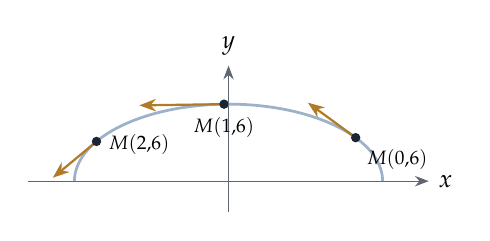
\begin{tikzpicture}
\begin{axis}[courbe,width=0.55\linewidth,xmin=-2.6,xmax=2.6,ymin=-0.4,ymax=1.5,xtick=\empty,ytick=\empty]
\addplot[reste,domain=0:pi,samples=150]({2*cos(x)},{sin(x)});
\draw[-{Stealth[length=6pt]},Ocre,thick] (axis cs:1.6507,0.5646)--(axis cs:1.030,1.019);
\draw[-{Stealth[length=6pt]},Ocre,thick] (axis cs:-0.0584,0.9996)--(axis cs:-1.158,0.9835);
\draw[-{Stealth[length=6pt]},Ocre,thick] (axis cs:-1.7138,0.5155)--(axis cs:-2.281,0.044);
\node[pt] at (axis cs:1.6507,0.5646) {}; \node[pt] at (axis cs:-0.0584,0.9996) {}; \node[pt] at (axis cs:-1.7138,0.5155) {};
\node[font=\scriptsize,anchor=north west] at (axis cs:1.67,0.54) {$M(0{,}6)$};
\node[font=\scriptsize,anchor=north] at (axis cs:-0.06,0.95) {$M(1{,}6)$};
\node[font=\scriptsize,anchor=west] at (axis cs:-1.68,0.48) {$M(2{,}6)$};
\end{axis}
\end{tikzpicture}
\caption{La trajectoire $f(t)=(2\cos t,\sin t)$, $t\in[0,\pi]$, et trois vecteurs vitesse $f'(t)$ (réduits de moitié).}\label{fig:vitesse}
\end{figure}

\begin{lecture}
Chaque flèche ocre part de la position $M(t)$ et représente $f'(t)=(-2\sin t,\cos t)$. On observe trois choses : la flèche est
\emph{tangente} à la trajectoire ; elle est orientée dans le \emph{sens du mouvement} quand $t$ augmente (ici de droite à
gauche) ; sa \emph{longueur} est la vitesse scalaire, plus grande au sommet ($\|f'(1{,}6)\|\approx2$) que sur les côtés
($\|f'(0{,}6)\|\approx1{,}4$). Ces trois informations sont celles dont on a besoin pour tracer une courbe.
\end{lecture}

\marge{Ensemble}
\begin{exemple}[mouvement circulaire uniforme]
Pour $f(t)=(R\cos\omega t,R\sin\omega t)$, calculer $f'$, $f''$ et $f\cdot f'$. Interpréter.
\chercher
$f'(t)=R\omega(-\sin\omega t,\cos\omega t)$, $f''(t)=-\omega^2f(t)$ et $f\cdot f'=0$. La vitesse scalaire $R|\omega|$ est
constante, l'accélération est dirigée vers le centre, la vitesse est orthogonale au rayon.
\end{exemple}

\rappel{développements limités en $0$} $e^t=1+t+\frac{t^2}2+\frac{t^3}6+o(t^3)$,\quad $\sin t=t-\frac{t^3}6+o(t^3)$,\quad
$\cos t=1-\frac{t^2}2+o(t^3)$.

\marge{Expliquer}
La formule de Taylor--Young s'écrit, elle aussi, coordonnée par coordonnée :
\[f(t_0+h)=f(t_0)+hf'(t_0)+\frac{h^2}2f''(t_0)+\dots+\frac{h^k}{k!}f^{(k)}(t_0)+o(h^k).\]

\begin{astuce}
On l'utilise surtout dans l'autre sens : on écrit le développement limité de $x$ et de $y$ avec les formules usuelles,
on regroupe les termes de même degré en vecteurs, et le coefficient de $h^k$ donne $\frac{f^{(k)}(t_0)}{k!}$. On obtient
ainsi plusieurs dérivées d'un coup, sans dériver. Ce sera l'outil principal de l'étude des points singuliers.
\end{astuce}

\marge{Ensemble}
\begin{exemple}
Pour $f(t)=(e^t,\sin t)$ en $0$ : $f(t)=(1,0)+t\,(1,1)+t^2\left(\tfrac12,0\right)+t^3\left(\tfrac16,-\tfrac16\right)+o(t^3)$,
d'où $f'(0)=(1,1)$, $f''(0)=(1,0)$ et $f'''(0)=(1,-1)$.
\end{exemple}

\marge{Seul}
\begin{exo}{fv-der}{1}{dériver une fonction vectorielle}
Calculer $f'$ et $f''$ pour $f(t)=(\cos2t,\ te^t)$.
\end{exo}
\coupdepouce{dériver chaque coordonnée séparément ; pour $te^t$, utiliser la dérivée d'un produit.}

% ---------------------------------------------------------------------
\Etape{7}{15 min}{Tangente en un point}{reconnaître un point régulier et écrire l'équation de la tangente.}

\pourquoi Pour tracer une courbe, on place quelques points, mais surtout la \emph{direction} de la courbe en ces points :
c'est la tangente. Un tracé sans tangentes est presque toujours faux près des points remarquables.

\marge{Expliquer}
L'ensemble $\Gamma=\{M(t),\ t\in I\}$ est le \emph{support} de la courbe. La tangente en $M(t_0)$ est la position limite des
cordes $\big(M(t_0)M(t)\big)$. Une corde est dirigée par $\frac{f(t)-f(t_0)}{t-t_0}$, qui tend vers $f'(t_0)$ : si ce vecteur
n'est pas nul, il dirige la tangente.

\begin{figure}[H]
\centering
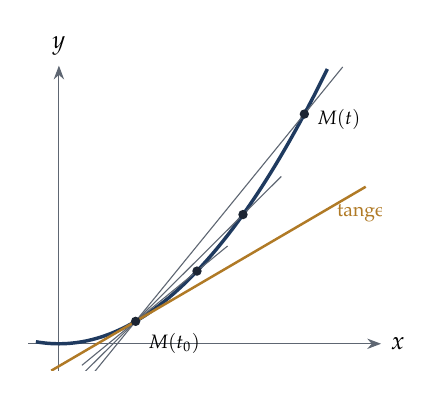
\begin{tikzpicture}
\begin{axis}[courbe,width=0.5\linewidth,xmin=-0.2,xmax=2.1,ymin=-0.3,ymax=3.1,xtick=\empty,ytick=\empty,axis equal image=false,height=0.45\linewidth]
\addplot[arcetude,domain=-0.15:1.75,samples=100]({x},{x^2});
\addplot[Gris,thin,domain=0.15:1.85,samples=2]{0.25+2.1*(x-0.5)};
\addplot[Gris,thin,domain=0.15:1.45,samples=2]{0.25+1.7*(x-0.5)};
\addplot[Gris,thin,domain=0.15:1.1,samples=2]{0.25+1.4*(x-0.5)};
\addplot[tgte,domain=-0.05:2.0,samples=2]{x-0.25};
\node[pt] at (axis cs:0.5,0.25) {}; \node[font=\scriptsize,anchor=north west] at (axis cs:0.52,0.22) {$M(t_0)$};
\node[pt] at (axis cs:1.6,2.56) {}; \node[pt] at (axis cs:1.2,1.44) {}; \node[pt] at (axis cs:0.9,0.81) {};
\node[font=\scriptsize,anchor=west] at (axis cs:1.62,2.5) {$M(t)$};
\node[font=\scriptsize,Ocre,anchor=west] at (axis cs:1.75,1.45) {tangente};
\end{axis}
\end{tikzpicture}
\caption{Sur la parabole $(t,t^2)$, les cordes issues de $M(t_0)$, $t_0=\frac12$, pivotent vers la tangente quand $t\to t_0$.}\label{fig:cordes}
\end{figure}

\begin{lecture}
Les droites grises joignent $M(t_0)$ à $M(t)$ pour trois valeurs de $t$ de plus en plus proches de $t_0$ : leurs pentes
($2{,}1$ ; $1{,}7$ ; $1{,}4$) diminuent et se rapprochent de $1$, la pente de la droite ocre. Chaque corde est dirigée par
$\frac{f(t)-f(t_0)}{t-t_0}$, le taux d'accroissement de $f$ ; quand $t\to t_0$, ce vecteur tend vers $f'(t_0)=(1,1)$. La
tangente est donc la droite passant par $M(t_0)$ et dirigée par $f'(t_0)$ --- à condition que ce vecteur ne soit pas nul.
\end{lecture}

\begin{definition}
Le point $M(t_0)$ est \emph{régulier} si $f'(t_0)\neq\ve0$, \emph{stationnaire} si $f'(t_0)=\ve0$.
\end{definition}

\rappel{colinéarité et déterminant, chapitre 1} Un point $M$ est sur la droite passant par $A$ et dirigée par $\ve u\neq\ve0$ si et seulement si
$\vv{AM}$ et $\ve u$ sont colinéaires, c'est-à-dire $\det(\vv{AM},\ve u)=0$.

\begin{theoreme}\label{thm:tgte}
En un point régulier $M(t_0)$, la courbe admet une tangente dirigée par $f'(t_0)$, d'équation
\begin{equation}\label{eq:tgte}
\det\big(\vv{M(t_0)M},f'(t_0)\big)=0\iff y'(t_0)\big(x-x(t_0)\big)-x'(t_0)\big(y-y(t_0)\big)=0.
\end{equation}
\end{theoreme}

Cette forme ne demande aucune division et convient aussi aux tangentes verticales. En un point régulier, la tangente est
horizontale si $y'(t_0)=0$, verticale si $x'(t_0)=0$.

Si $x'(t_0)\neq0$, on peut diviser : la tangente a pour \emph{pente} $p=\dfrac{y'(t_0)}{x'(t_0)}$ et pour équation
$y=y(t_0)+p\,\big(x-x(t_0)\big)$. Un graphe $y=g(x)$ est la courbe paramétrée $t\mapsto\big(t,g(t)\big)$ : la pente vaut
alors $\frac{g'(t)}1$, et l'on retrouve la tangente bien connue $y=g(a)+g'(a)(x-a)$.

\begin{votrecours}
\textbf{Équation ou paramétrage.} Une courbe n'a pas toujours d'équation $y=g(x)$ : à une abscisse peuvent correspondre
plusieurs points (un cercle, une boucle). On distingue l'\emph{équation cartésienne}, $\{(x,y)\mid F(x,y)=0\}$, et la
\emph{représentation paramétrique}, $\{M(t)\mid t\in I\}$. Par exemple, la droite passant par $A(1,2)$ et $B(2,-2)$ a pour
équation $y=-4x+6$ (obtenue par $\det(\vv{AB},\vv{AM})=0$) et pour paramétrage $t\mapsto(t,-4t+6)$, ou
$t\mapsto A+t\,\vv{AB}$ ; le cercle de centre $\Omega(1,2)$ et de rayon $R$ a pour équation $(x-1)^2+(y-2)^2=R^2$ et pour
paramétrage $\theta\mapsto(1+R\cos\theta,2+R\sin\theta)$, $\theta\in\,]-\pi,\pi]$ ; son demi-cercle supérieur est le graphe
de $x\mapsto2+\sqrt{R^2-(x-1)^2}$.

\textbf{Tangente.} Le cours définit la tangente en $M(t_0)$ comme la limite, lorsque $h\to0$, des droites
$M(t_0)+\vect(\ve u_h)$, où $\ve u_h=\frac{\vv{M(t_0)M(t_0+h)}}{\|\vv{M(t_0)M(t_0+h)}\|}$ est un vecteur \emph{unitaire}
dirigeant la corde (c'est aussi la définition du programme). On normalise parce que $\vv{M(t_0)M(t_0+h)}$ tend vers
$\ve0$ et ne fournit donc, seul, aucune direction. La formule de Taylor--Young donne $\vv{M(t_0)M(t_0+h)}=h\,f'(t_0)+o(h)$,
donc, si $f'(t_0)\neq\ve0$,
\[\ve u_h=\frac{h\big(f'(t_0)+o(1)\big)}{|h|\,\big(\|f'(t_0)\|+o(1)\big)}\longrightarrow\pm\frac{f'(t_0)}{\|f'(t_0)\|}
\quad(h\to0^\pm),\]
et les deux limites dirigent la même droite : c'est la démonstration du théorème~\ref{thm:tgte}.
\end{votrecours}

\marge{Ensemble}
\begin{exemple}[une parabole]
Pour $f(t)=(t,t^2)$ en $t_0=1$ : $M(1)=(1,1)$, $f'(1)=(1,2)$, d'où la tangente $2(x-1)-(y-1)=0$, soit $y=2x-1$. On
retrouve la tangente au graphe de $x\mapsto x^2$.
\end{exemple}

\marge{Questionner}
\question{Pour $f(t)=(t^2-2t,\ t^3-3t)$, en quels points la tangente est-elle horizontale ? verticale ?}

\begin{exemple}
On \emph{factorise} les dérivées : $x'(t)=2(t-1)$ et $y'(t)=3(t-1)(t+1)$.
\chercher
\begin{itemize}
\item En $t=-1$ : $y'=0$ et $x'=-4\neq0$, tangente horizontale au point $(3,2)$.
\item En $t=1$ : $x'=y'=0$, le point $(-1,-2)$ est stationnaire ; le théorème ne s'applique pas.
\end{itemize}
\end{exemple}

\begin{attention}
« $x'(t_0)=0$, donc la tangente est verticale » n'est vrai qu'en un point \emph{régulier}, c'est-à-dire si
$y'(t_0)\neq0$. On vérifie toujours l'autre dérivée.
\end{attention}

\begin{reflexe}
Factoriser $x'$ et $y'$ dès qu'on les a calculées : on lit d'un coup les tangentes horizontales, verticales et les points
stationnaires, et l'on prépare le tableau de variations.
\end{reflexe}

\marge{Expliquer}
\begin{exemple}[et en un point stationnaire ?]
Pour $f(t)=(t^2,t^3)$, $f'(0)=\ve0$. Les cordes sont dirigées par $\frac{(t^2,t^3)}{t^2}=(1,t)\to(1,0)$ : il y a bien
une tangente horizontale en $O$, mais elle n'est pas donnée par $f'(0)$. La courbe forme une pointe ; l'étude de ces
points est l'objet de la séance 2.
\end{exemple}

\begin{figure}[H]
\centering
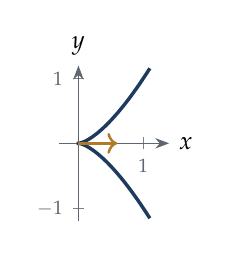
\begin{tikzpicture}
\begin{axis}[courbe,width=0.34\linewidth,xmin=-0.3,xmax=1.4,ymin=-1.2,ymax=1.2,xtick={1},ytick={-1,1}]
\addplot[arcetude,domain=-1.05:1.05,samples=150]({x^2},{x^3});
\draw[tgte,->](axis cs:0,0)--(axis cs:0.6,0);
\end{axis}
\end{tikzpicture}
\caption{La courbe $(t^2,t^3)$ forme une pointe en son point stationnaire.}
\end{figure}

\marge{Seul}
\begin{exo}{tg-a}{1}{équation de tangente}
Donner une équation de la tangente en $M(t_0)$ à la courbe $f(t)=(t,e^{-t^2})$, puis à l'ellipse
$f(t)=(\cos t,2\sin t)$.
\end{exo}
\coupdepouce{vérifier d'abord que $f'(t_0)\neq\ve0$, puis écrire $\det\big(\vv{M(t_0)M},f'(t_0)\big)=0$ et simplifier par $\cos^2t_0+\sin^2t_0=1$.}

\pointarret{la dérivation et la tangente sont acquises. Reprise à l'étape 8, ou directement à l'étape 10 du chapitre 5 si le temps manque.}

% ---------------------------------------------------------------------
\Etape{8}{10 min}{Réduire l'intervalle d'étude}{repérer les symétries d'une courbe avant tout calcul.}

\pourquoi Étudier une courbe demande des dérivées, un tableau de variations, des limites. Si la courbe est symétrique,
la moitié de ce travail est inutile. On cherche donc les symétries \emph{avant} de dériver.

\rappel{symétries} Le symétrique de $(x,y)$ est $(x,-y)$ par rapport à $(Ox)$, $(-x,y)$ par rapport à $(Oy)$, $(-x,-y)$ par
rapport à $O$, $(y,x)$ par rapport à la droite $y=x$.

\marge{Expliquer}
On compare $f(\varphi(t))$ et $f(t)$ pour quelques transformations simples du paramètre : $t+T$, $-t$, $\pi-t$. Si
$M(\varphi(t))$ est le symétrique de $M(t)$, on étudie la courbe sur une moitié du domaine, puis on complète le tracé.

\begin{table}[H]
\centering
\renewcommand{\arraystretch}{1.25}
\begin{tabular}{lll}
\toprule
\sffamily Relation constatée & \sffamily Transformation du support & \sffamily Réduction\\\midrule
$f(t+T)=f(t)$ & aucune (périodicité) & intervalle de longueur $T$\\
$x$ paire, $y$ impaire & symétrie d'axe $(Ox)$ & $t\geq0$\\
$x$ impaire, $y$ paire & symétrie d'axe $(Oy)$ & $t\geq0$\\
$x$ et $y$ impaires & symétrie de centre $O$ & $t\geq0$\\\bottomrule
\end{tabular}
\caption{Invariances usuelles.}
\end{table}

\marge{Ensemble}
\begin{exemple}[deux symétries successives]\label{ex:huit}
Réduire l'intervalle d'étude de $f(t)=(\sin t,\sin2t)$.
\chercher
\etape{Périodicité} $f$ est $2\pi$-périodique : on part de $[-\pi,\pi]$.
\etape{Première symétrie} $f(-t)=-f(t)$ : symétrie de centre $O$ ; on se ramène à $[0,\pi]$.
\etape{Seconde symétrie} $t\mapsto\pi-t$ échange $[0,\frac\pi2]$ et $[\frac\pi2,\pi]$, et $f(\pi-t)=(\sin t,-\sin2t)$ :
symétrie d'axe $(Ox)$ ; on se ramène à $[0,\frac\pi2]$.
\etape{Reconstitution} On trace l'arc de $[0,\frac\pi2]$, on le complète par la symétrie d'axe $(Ox)$, puis par la symétrie
de centre $O$.
\end{exemple}

\begin{figure}[H]
\centering
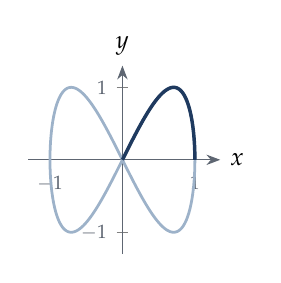
\begin{tikzpicture}
\begin{axis}[courbe,width=0.38\linewidth,xmin=-1.3,xmax=1.35,ymin=-1.3,ymax=1.3,xtick={-1,1},ytick={-1,1}]
\addplot[reste,domain=0:2*pi,samples=300]({sin(x)},{sin(2*x)});
\addplot[arcetude,domain=0:pi/2,samples=150]({sin(x)},{sin(2*x)});
\end{axis}
\end{tikzpicture}
\caption{La courbe $(\sin t,\sin2t)$ ; en trait foncé, l'arc d'étude.}
\end{figure}

\begin{attention}
Les symétries se reportent dans l'ordre \emph{inverse} des réductions, et l'on vérifie que chaque transformation du
paramètre envoie la partie étudiée sur la partie manquante : ici $t\mapsto\pi-t$ envoie bien $[0,\frac\pi2]$ sur
$[\frac\pi2,\pi]$.
\end{attention}

% ---------------------------------------------------------------------
\Etape{9}{5 min}{Faire le point}{vérifier ce que l'étudiant sait refaire seul et fixer le travail de la semaine.}

\marge{Questionner}
À la fin de la séance, l'étudiant doit savoir, \emph{sans le livre} :
\begin{enumerate}
\item tester une colinéarité, une coplanarité ou une base par un déterminant ;
\item calculer un déterminant par le pivot, en tenant compte des échanges et des facteurs ;
\item utiliser $\det(AB)$, $\det(\lambda A)$, $\det A^{-1}$ ;
\item factoriser un déterminant à paramètre ;
\item dériver une fonction vectorielle et écrire la tangente en un point régulier ;
\item repérer les parités de $x$ et $y$ pour réduire l'intervalle d'étude.
\end{enumerate}

\paragraph{Travail pour la semaine} Le chapitre~\ref{sec:perso}, dans l'ordre, en insistant sur les points de la liste qui
ont posé difficulté, puis ses exercices de bilan. Le chapitre~\ref{sec:approf} est facultatif. Relire les étapes 6 et 7
avant la séance 2.

\begin{essentiel}\label{ess:2}
\begin{itemize}
\item On dérive une fonction vectorielle coordonnée par coordonnée : $f'=(x',y')$.
\item Un développement limité de $x$ et $y$ donne d'un coup les dérivées successives de $f$.
\item En un point régulier ($f'(t_0)\neq\ve0$), la tangente a pour équation $y'(t_0)(x-x_0)-x'(t_0)(y-y_0)=0$.
\item Tangente horizontale si $y'=0\neq x'$, verticale si $x'=0\neq y'$ ; si $x'=y'=0$, on ne peut rien conclure.
\item Avant de dériver, on cherche périodicité et symétries, et l'on complète le tracé dans l'ordre inverse.
\end{itemize}
\end{essentiel}

% =====================================================================
%              PARTIE 3 — TRAVAIL PERSONNEL APRÈS LA SÉANCE
% =====================================================================
\clearpage
\section{Après la séance : consolidation et bilan}\label{sec:perso}

Ce chapitre prolonge la séance. Ses exercices suivent l'ordre des étapes : chaque série ne demande que ce qui a été vu
jusqu'à l'étape indiquée, et varie les situations plutôt que de répéter le même calcul. Il vaut mieux en traiter peu,
mais entièrement et sans regarder le corrigé, que beaucoup en les survolant. Les exercices de bilan, à la fin,
mélangent les notions : c'est à l'étudiant d'identifier la bonne méthode.

\ouverture{%
\begin{itemize}
\item Refaire seul les calculs de la séance.
\item Rencontrer chaque technique dans une situation nouvelle.
\item Vérifier ses acquis sur des exercices qui mélangent les notions.
\end{itemize}}{%
\begin{itemize}
\item Chapitres 1 et 2.
\end{itemize}}{Environ trois heures de travail personnel dans la semaine.}

\serie{Après les étapes 1 et 2 --- dimension 2 et 3}

\begin{exo}{d2-col}{1}{colinéarité}
Les vecteurs $(6,-9)$ et $(-4,6)$ sont-ils colinéaires ? Même question pour $(1,3)$ et $(3,1)$.
\end{exo}
\begin{exo}{d2-aire}{2}{aire d'un parallélogramme}
Calculer l'aire du parallélogramme $ABCD$ avec $A(0,0)$, $B(3,1)$ et $D(1,2)$. Quelles sont les coordonnées de $C$ ?
\end{exo}
\begin{exo}{d3-calc}{2}{calcul en dimension 3}
Calculer $\dt{2&0&1\\1&3&0\\0&1&4}$ de deux façons : par la formule~\eqref{eq:det3}, puis par la règle de Sarrus.
\end{exo}

\serie{Après l'étape 3 --- calcul par le pivot}

\begin{exo}{m-tri}{1}{matrice triangulaire, colonnes proportionnelles}
Calculer, sans développer, $\dt{3&0&0\\7&-1&0\\2&5&2}$ et $\dt{1&-2&4\\2&-4&1\\-1&2&3}$.
\end{exo}
\begin{exo}{m-erreur}{3}{analyser une erreur}
Un élève écrit : « avec $C_1\leftarrow C_1-C_2$ puis $C_2\leftarrow C_2-C_1$, le déterminant
$\dt{a&b\\c&d}$ devient $\dt{a-b&b-a\\c-d&d-c}$, qui est nul ; donc tout déterminant $2\times2$ est nul. » Où est
l'erreur ? Effectuer correctement ces deux opérations successives et vérifier que le déterminant obtenu vaut bien
$ad-bc$.
\end{exo}
\begin{exo}{m-circ4}{2}{choisir entre pivot et somme constante}
Calculer $D=\dt{1&2&3&4\\2&3&4&1\\3&4&1&2\\4&1&2&3}$ de deux façons : par le pivot de Gauss, puis en remarquant une
propriété des lignes. Laquelle est la plus sûre ?
\end{exo}

\serie{Après l'étape 4 --- inversibilité et bases}

\rappel{formule du binôme} $(X+a)^k=\sum_{i=0}^k\binom ki a^{k-i}X^i$ ; le coefficient de $X^k$ vaut $1$.

\begin{exo}{f-base}{1}{déterminant et base}
La famille $\big((1,2,1),(2,1,0),(1,1,1)\big)$ est-elle une base de $\R^3$ ?
\end{exo}
\begin{exo}{f-poly}{2}{base de polynômes}
Montrer que $\big(1,\ 1+X,\ 1+X+X^2,\ 1+X+X^2+X^3\big)$ est une base de $\R_3[X]$.
\end{exo}
\begin{exo}{f-tau}{2}{matrice d'un endomorphisme}
Soit $n\geq1$ et $\tau:P\mapsto P(X+1)$ sur $\R_n[X]$. Calculer $\det\tau$, puis $\det(\tau-\Id)$. Calculer également
le déterminant de la dérivation $D:P\mapsto P'$ sur $\R_n[X]$, et interpréter.
\end{exo}

\serie{Après l'étape 5 --- développement et paramètres}

\begin{exo}{m-dev}{2}{développement selon une ligne ou une colonne}
Calculer $\dt{0&0&3\\0&2&1\\1&4&5}$ et $\dt{1&0&0&2\\0&3&0&0\\4&1&2&0\\0&0&0&1}$.
\end{exo}
\begin{exo}{m-inv}{2}{inversibilité avec paramètre}
Pour quelles valeurs de $a\in\R$ la matrice $\begin{pmatrix}1&a&0\\a&1&a\\0&a&1\end{pmatrix}$ est-elle inversible ?
\end{exo}
\begin{exo}{t-somme}{2}{somme constante}
Calculer $\dt{1&2&2\\2&1&2\\2&2&1}$, puis $\dt{0&1&1&1\\1&0&1&1\\1&1&0&1\\1&1&1&0}$.
\end{exo}
\begin{exo}{t-fact}{2}{différences de lignes, factorisation}
Calculer sous forme factorisée $\dt{1&a&bc\\1&b&ca\\1&c&ab}$.
\end{exo}
\begin{exo}{t-circ}{3}{somme constante, identité remarquable}
Calculer sous forme factorisée le déterminant circulant $D=\dt{a&b&c\\c&a&b\\b&c&a}$, puis déterminer, pour $a,b,c$
réels, à quelle condition il est nul. On pourra exprimer $a^2+b^2+c^2-ab-bc-ca$ à l'aide de carrés.
\end{exo}
\begin{exo}{m-lettres}{2}{développer selon une colonne creuse}
Calculer $\Delta=\dt{a&1&0&x\\b&2&1&y\\c&0&0&z\\d&1&0&t}$ en développant selon une colonne bien choisie. Pourquoi $y$
n'apparaît-il pas dans le résultat ?
\end{exo}

\serie{Après l'étape 6 --- fonctions vectorielles}

\rappel{développements limités utiles} $\ln(1+u)=u-\frac{u^2}2+o(u^2)$ et $\arctan u=u-\frac{u^3}3+o(u^3)$ en $0$.

\begin{exo}{fv-vit}{2}{vitesse scalaire}
Calculer la vitesse scalaire $\|f'(t)\|$ du mouvement $f(t)=(t-\sin t,\ 1-\cos t)$, et la simplifier à l'aide de la
formule $1-\cos t=2\sin^2\frac t2$. À quels instants la vitesse est-elle nulle ?
\end{exo}
\begin{exo}{fv-td1}{2}{classe $\mathcal C^\infty$ ; dérivées par développement limité}
Soit $f(t)=\big(\ln(1+t^2),\arctan(2t)\big)$. Justifier que $f$ est de classe $\mathcal C^\infty$ sur $\R$, étudier
l'annulation de $f'$, puis calculer $f^{(k)}(0)$ pour $k\in\ient03$ à l'aide d'un développement limité.
\end{exo}
\begin{exo}{fv-norme}{3}{dérivée d'un produit scalaire ; interprétation}
Soit $f:I\to\R^2$ de classe $\mathcal C^1$, $f(t)=\vv{OM(t)}$, telle que $\|f(t)\|=\alpha>0$ pour tout $t\in I$.
\begin{enumerate}
\item Montrer que $\vv{OM(t)}$ et $f'(t)$ sont orthogonaux pour tout $t$. On dérivera $f\cdot f$.
\item Quels résultats classiques de géométrie et de mécanique retrouve-t-on ?
\item Montrer de même que si la vitesse scalaire $\|f'\|$ est constante, l'accélération est orthogonale à la vitesse.
\end{enumerate}
\end{exo}

\serie{Après l'étape 7 --- tangentes}

\begin{exo}{tg-par}{2}{tangente parallèle à une direction}
Soit $f(t)=(t^3,t^2)$. Déterminer les points réguliers où la tangente est parallèle à la droite $y=x$.
\end{exo}
\begin{exo}{tg-c}{2}{régularité, factorisation de $f'$}
Préciser les points stationnaires de $f(t)=\left(t+\frac1t,\ t\ln t-t\right)$, $t>0$, et donner une équation de la
tangente en un point régulier.
\end{exo}
\begin{exo}{tg-d}{2}{factorisation de $f'$}
Mêmes questions pour $f(t)=(\cos t,\sin^3t)$, $t\in\R$.
\end{exo}

\serie{Après l'étape 8 --- réduction du domaine}

\begin{exo}{red-a}{2}{périodicité, symétries}
Déterminer un domaine d'étude et les symétries permettant de compléter le tracé de $f(t)=(\cos3t,\sin2t)$.
\end{exo}
\begin{exo}{red-b}{2}{domaine de définition, symétries}
Même question pour $f(t)=(\tan t,\cos t)$.
\end{exo}
\begin{exo}{red-c}{3}{reconnaître une courbe au lieu de réduire}
Même question pour $f(t)=(\cos t+\sin t,\ \cos t-\sin t)$. On calculera d'abord $x^2+y^2$.
\end{exo}

\serie{Exercices de bilan de la séance 1}

Ces trois exercices ne disent pas quelle méthode employer. Avant de calculer, on se demande : quelle question
est posée, quel outil y répond, quelle structure présente le calcul ?

\begin{exo}{b-famille}{3}{base, paramètre, factorisation}
Pour $a\in\R$, on considère les vecteurs $\ve u=(1,a,a^2)$, $\ve v=(a,1,a)$ et $\ve w=(a^2,a,1)$. Pour quelles valeurs
de $a$ forment-ils une base de $\R^3$ ? On cherchera une opération sur les lignes qui crée deux zéros d'un coup.
\end{exo}
\begin{exo}{b-J}{3}{somme constante, inversibilité}
Soit $J\in\Mn{\R}$ la matrice dont tous les coefficients valent $1$, et $\lambda\in\R$.
\begin{enumerate}
\item Calculer $\det(J+\lambda I_n)$.
\item Pour quelles valeurs de $\lambda$ la matrice $J+\lambda I_n$ est-elle inversible ?
\item En déduire que, pour $n\geq2$, la matrice $J-I_n$ est inversible.
\end{enumerate}
\end{exo}
\begin{exo}{b-cercle}{2}{élimination du paramètre, régularité, tangente}
Soit $f(t)=\left(\dfrac{2t}{1+t^2},\dfrac{1-t^2}{1+t^2}\right)$, $t\in\R$.
\begin{enumerate}
\item Montrer que le support est inclus dans le cercle unité $\mathcal C$.
\item Montrer que tout point de $\mathcal C$ autre que $(0,-1)$ est atteint. On pourra poser $t=\frac{x}{1+y}$.
\item Montrer que la courbe est régulière et que la tangente en $M(t)$ est orthogonale à $\vv{OM(t)}$.
\end{enumerate}
\end{exo}

% =====================================================================
%                   PARTIE 4 — APPROFONDISSEMENT
% =====================================================================
\clearpage
\section{Déterminants : approfondissement}\label{sec:approf}

La séance a mis en place l'essentiel. Ce chapitre présente des résultats et des techniques qui ne sont pas
indispensables à une première compréhension, mais qui sont au programme de PT et reviennent régulièrement dans les
problèmes de concours. Chaque section commence par le court passage de cours qui rend ses exercices abordables, en
partant toujours d'un cas déjà rencontré pendant la séance.

\ouverture{%
\begin{itemize}
\item Traduire alignement, coplanarité, aires et volumes en déterminants.
\item Utiliser les règles de calcul sans calculer de coefficient.
\item Maîtriser le déterminant de Vandermonde et ses applications.
\item Calculer un déterminant d'ordre $n$ par récurrence, par différences successives, ou en exploitant les zéros.
\item Traiter toutes les techniques du cours et du TD de la classe, y compris hors programme (comatrice).
\end{itemize}}{%
\begin{itemize}
\item Chapitre 1 entier.
\item Exercices du chapitre 3 sur les déterminants.
\end{itemize}}{Environ deux heures de travail personnel, section par section.}

\begin{commencer}
Ce chapitre utilise les résultats suivants du chapitre 1, rassemblés ici pour pouvoir le commencer directement.
\begin{itemize}
\item Une transvection $C_i\leftarrow C_i+\lambda C_j$ ne change pas le déterminant ; un échange change son signe ; une
      dilatation $C_i\leftarrow\lambda C_i$ le multiplie par $\lambda$. Mêmes règles sur les lignes.
\item Le déterminant d'une matrice triangulaire est le produit des coefficients diagonaux.
\item $\det(AB)=\det A\det B$, $\det(A^T)=\det A$, $\det(\lambda A)=\lambda^n\det A$ ; $A$ inversible $\iff\det A\neq0$.
\item $n$ vecteurs d'un espace de dimension $n$ forment une base si et seulement si leur déterminant est non nul.
\item On peut développer selon une ligne ou une colonne : $\det A=\sum_j(-1)^{i+j}a_{i,j}\Delta_{i,j}$.
\item Si toutes les lignes ont la même somme, $C_1\leftarrow C_1+\dots+C_n$ fait apparaître ce facteur commun ;
      en particulier, le déterminant d'ordre $n$ à diagonale $a$ et autres coefficients $b$ vaut $(a+(n-1)b)(a-b)^{n-1}$.
\end{itemize}
\end{commencer}

% ---------------------------------------------------------------------
\subsection{Applications géométriques}

Les étapes 1 et 2 ont montré que le déterminant mesure des aires et des volumes orientés. Il traduit donc directement
les questions d'alignement et de coplanarité, et permet d'écrire l'équation d'une droite ou d'un plan sans résoudre de
système : c'est un gain de temps considérable dans les exercices de géométrie. Les aires et volumes supposent une base orthonormée ; le triangle est la
moitié du parallélogramme, le tétraèdre le sixième du parallélépipède.

\begin{table}[H]
\centering
\renewcommand{\arraystretch}{1.3}
\begin{tabular}{p{0.44\linewidth}p{0.46\linewidth}}
\toprule
Propriété géométrique & Traduction\\\midrule
$A$, $B$, $C$ alignés & $\det(\vv{AB},\vv{AC})=0$\\
$M$ appartient à la droite $(AB)$ & $\det(\vv{AM},\vv{AB})=0$\\
aire du triangle $ABC$ & $\frac12\big|\det(\vv{AB},\vv{AC})\big|$\\\midrule
$M$ appartient au plan $(ABC)$ & $\det(\vv{AM},\vv{AB},\vv{AC})=0$\\
droites $(A,\ve u)$ et $(B,\ve v)$ coplanaires & $\det(\vv{AB},\ve u,\ve v)=0$\\
volume du tétraèdre $ABCD$ & $\frac16\big|\det(\vv{AB},\vv{AC},\vv{AD})\big|$\\\bottomrule
\end{tabular}
\caption{Traduction de propriétés géométriques par des déterminants.}
\end{table}

\begin{exemple}[équation d'un plan]
Le plan passant par $A(1,0,0)$, $B(0,1,0)$ et $C(0,0,1)$ s'obtient sans résoudre de système : avec
$\vv{AB}=(-1,1,0)$ et $\vv{AC}=(-1,0,1)$, en développant selon la première colonne,
\[M(x,y,z)\in(ABC)\iff\dt{x-1&-1&-1\\y&1&0\\z&0&1}=0\iff x+y+z=1,\]
car ce déterminant vaut $(x-1)+y+z$.
\end{exemple}

\begin{exo}{geo-aire}{1}{aire et volume}
\begin{enumerate}
\item Calculer l'aire du triangle de sommets $A(1,1)$, $B(4,2)$, $C(2,5)$.
\item Calculer le volume du tétraèdre de sommets $O$, $A(1,0,0)$, $B(0,2,0)$, $C(1,1,3)$.
\end{enumerate}
\end{exo}
\begin{exo}{geo-cop}{2}{coplanarité de quatre points}
Les points $A(1,0,0)$, $B(0,1,0)$, $C(0,0,1)$ et $D(1,1,-1)$ sont-ils coplanaires ?
\end{exo}
\begin{exo}{b-plan}{2}{géométrie dans l'espace}
On considère les points $A(1,1,0)$, $B(2,0,1)$, $C(0,1,1)$ et $D(1,0,2)$.
\begin{enumerate}
\item Montrer que $A$, $B$, $C$ ne sont pas alignés et déterminer une équation du plan $(ABC)$.
\item Le point $D$ appartient-il à ce plan ?
\item Calculer le volume du tétraèdre $OABC$.
\end{enumerate}
\end{exo}
\begin{exo}{geo-sym}{3}{déterminant de taille 3 et géométrie plane}
Montrer que les points $M(x,y)$, $M'(x',y')$, $M''(x'',y'')$ sont alignés si et seulement si
\[\dt{x&x'&x''\\y&y'&y''\\1&1&1}=0.\]
\end{exo}
\begin{exo}{geo-droites}{3}{droites de l'espace}
Soit $\mathcal D_1$ la droite passant par $A(1,0,0)$ et dirigée par $\ve u=(1,1,0)$, et, pour $m\in\R$, $\mathcal D_m$ la
droite passant par $B(0,1,m)$ et dirigée par $\ve v=(0,1,1)$. Pour quelle valeur de $m$ ces droites sont-elles
sécantes ? Déterminer alors leur point d'intersection.
\end{exo}

\paragraph{Distance de deux droites de l'espace} Le TD demande de calculer la distance de deux droites non parallèles
de l'espace ; c'est une application directe du produit mixte, qui mesure un volume (étape 2).

\begin{proposition}\label{prop:dist-droites}
Soient $\mathcal D_1=A+\vect(\ve u)$ et $\mathcal D_2=C+\vect(\ve v)$ deux droites non parallèles de l'espace (base
orthonormée directe). Il existe un unique couple $(H,K)\in\mathcal D_1\times\mathcal D_2$ tel que $(HK)$ soit
perpendiculaire aux deux droites, et
\[d(\mathcal D_1,\mathcal D_2)=HK=\frac{\big|\det(\vv{AC},\ve u,\ve v)\big|}{\|\ve u\wedge\ve v\|}.\]
Pour les droites $(AB)$ et $(CD)$, cela s'écrit $d=\dfrac{|\det(\vv{AB},\vv{CD},\vv{AC})|}{\|\vv{AB}\wedge\vv{CD}\|}$.
\end{proposition}

\begin{proof}
\begin{itemize}
\item \emph{Existence de $H$ et $K$.} Avec $H=A+s\ve u$ et $K=C+r\ve v$, les conditions $\vv{HK}\cdot\ve u=0$ et
      $\vv{HK}\cdot\ve v=0$ forment un système linéaire en $(s,r)$, de déterminant
      $-\big(\|\ve u\|^2\|\ve v\|^2-(\ve u\cdot\ve v)^2\big)=-\|\ve u\wedge\ve v\|^2\neq0$ : il a une unique solution.
\item \emph{$HK$ est la plus courte distance.} Pour $M\in\mathcal D_1$ et $N\in\mathcal D_2$,
      $\vv{MN}=\vv{HK}+(\vv{MH}+\vv{KN})$, où $\vv{MH}+\vv{KN}\in\vect(\ve u,\ve v)$ est orthogonal à $\vv{HK}$ ; par
      Pythagore, $MN^2=HK^2+\|\vv{MH}+\vv{KN}\|^2\geq HK^2$.
\item \emph{Formule.} $\det(\vv{AC},\ve u,\ve v)=(\ve u\wedge\ve v)\cdot\vv{AC}=(\ve u\wedge\ve v)\cdot(\vv{AH}+\vv{HK}+\vv{KC})
      =(\ve u\wedge\ve v)\cdot\vv{HK}$, car $\vv{AH}$ et $\vv{KC}$ sont colinéaires à $\ve u$ et $\ve v$, orthogonaux à
      $\ve u\wedge\ve v$. Comme $\vv{HK}$ est colinéaire à $\ve u\wedge\ve v$, ce produit scalaire vaut
      $\pm\|\ve u\wedge\ve v\|\,HK$.\qedhere
\end{itemize}
\end{proof}

\begin{figure}[H]
\centering
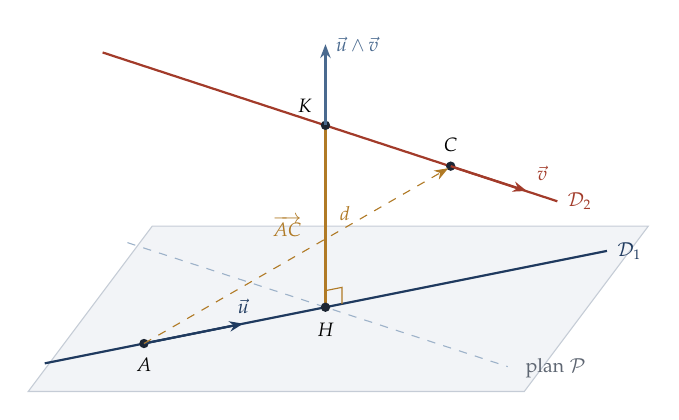
\begin{tikzpicture}[scale=1.05,>={Stealth[length=5pt]}]
\fill[Fond] (0,0)--(6,0)--(7.5,2)--(1.5,2)--cycle;
\draw[Filet] (0,0)--(6,0)--(7.5,2)--(1.5,2)--cycle;
\node[font=\scriptsize,Gris,anchor=south west] at (5.9,0.05) {plan $\mathcal P$};
% D1 dans le plan
\draw[Bleu,thick] (0.2,0.34)--(7.0,1.70) node[right,font=\scriptsize]{$\mathcal D_1$};
% projection de D2 dans le plan
\draw[BleuClair,dashed] (1.2,1.8)--(5.8,0.3);
% D2 au-dessus
\draw[Brique,thick] (0.9,4.1)--(6.4,2.3) node[right,font=\scriptsize]{$\mathcal D_2$};
% perpendiculaire commune
\draw[Ocre,thick] (3.595,1.019)--(3.595,3.219);
\draw[Ocre] (3.595,1.219)--(3.795,1.259)--(3.795,1.059);
\node[pt] at (3.595,1.019) {}; \node[font=\scriptsize,anchor=north] at (3.595,0.95) {$H$};
\node[pt] at (3.595,3.219) {}; \node[font=\scriptsize,anchor=south east] at (3.55,3.25) {$K$};
\node[font=\scriptsize,Ocre,anchor=west] at (3.65,2.15) {$d$};
% A, C et vecteurs
\node[pt] at (1.4,0.58) {}; \node[font=\scriptsize,anchor=north] at (1.4,0.52) {$A$};
\draw[->,Bleu,thick] (1.4,0.58)--(2.6,0.82) node[above,font=\scriptsize]{$\ve u$};
\node[pt] at (5.11,2.725) {}; \node[font=\scriptsize,anchor=south] at (5.11,2.78) {$C$};
\draw[->,Brique,thick] (5.11,2.725)--(6.03,2.425) node[above right,font=\scriptsize]{$\ve v$};
\draw[->,Ocre,dashed] (1.4,0.58)--(5.08,2.70) node[pos=0.55,above left,font=\scriptsize]{$\vv{AC}$};
\draw[->,BleuMoyen,thick] (3.595,3.219)--(3.595,4.2) node[right,font=\scriptsize]{$\ve u\wedge\ve v$};
\end{tikzpicture}
\caption{Deux droites non coplanaires, le plan $\mathcal P$ contenant $\mathcal D_1$ et parallèle à $\mathcal D_2$ (gris),
et la perpendiculaire commune $[HK]$ (ocre).}\label{fig:dist-droites}
\end{figure}

\begin{lecture}
Le plan grisé $\mathcal P$ contient $\mathcal D_1$ et est dirigé par $\ve u$ et $\ve v$ ; la droite $\mathcal D_2$ lui est
parallèle et « flotte » au-dessus, à la hauteur $d$ (son projeté sur $\mathcal P$ est en pointillés). Le vecteur
$\ve u\wedge\ve v$ est normal à $\mathcal P$. La distance cherchée est la hauteur de $C$ au-dessus de $\mathcal P$,
c'est-à-dire la longueur de la projection de $\vv{AC}$ sur la normale. Or, comme à l'étape 2,
$|\det(\vv{AC},\ve u,\ve v)|$ est le volume du parallélépipède construit sur $\ve u$, $\ve v$, $\vv{AC}$ : base
$\|\ve u\wedge\ve v\|$ fois hauteur $d$. On divise par la base pour obtenir la hauteur. Si le volume est nul, les deux
droites sont coplanaires, donc sécantes : on retrouve la dernière ligne du tableau.
\end{lecture}

\begin{exo}{geo-dist}{3}{distance de deux droites, coplanarité}
Soient $\mathcal D_1$ la droite passant par $A(1,0,0)$ dirigée par $\ve u=(1,1,0)$ et, pour $m\in\R$, $\mathcal D_m$ la
droite passant par $C_m(0,0,m)$ dirigée par $\ve v=(0,1,1)$.
\begin{enumerate}
\item Calculer la distance de $\mathcal D_1$ à $\mathcal D_m$. Pour quelle valeur de $m$ les droites sont-elles sécantes ?
\item Pour $m=2$, déterminer les points $H\in\mathcal D_1$ et $K\in\mathcal D_2$ tels que $(HK)$ soit perpendiculaire aux
      deux droites, et vérifier que $HK$ est bien la distance trouvée.
\end{enumerate}
\end{exo}

% ---------------------------------------------------------------------
\subsection{Propriétés globales et endomorphismes}

\pourquoi Certaines questions portent sur des matrices dont on ne connaît pas les coefficients : seule une relation
est donnée ($A^T=-A$, $A^2=-I_n$\dots). Ces questions se traitent sans calculer aucun coefficient, avec les seules règles de l'étape 4 :
$\det(AB)=\det A\det B$, $\det(A^T)=\det A$ et $\det(\lambda A)=\lambda^n\det A$. Par exemple, si $A^TA=I_n$, alors
$(\det A)^2=1$, donc $\det A=\pm1$.

Pour un endomorphisme, le déterminant ne dépend pas de la base : on choisit une base dans laquelle la matrice est
triangulaire, voire diagonale. Ainsi, la symétrie orthogonale de $\R^3$ par rapport au plan $x+y+z=0$ a pour matrice
$\mathrm{diag}(1,1,-1)$ dans une base formée de deux vecteurs du plan et du vecteur normal $(1,1,1)$ : son déterminant
vaut $-1$.

\begin{exo}{g-antisym}{2}{déterminant de la transposée, de $\lambda A$}
Montrer qu'une matrice antisymétrique réelle d'ordre impair n'est pas inversible.
\end{exo}
\begin{exo}{g-carre}{3}{multiplicativité du déterminant}
Soit $A\in\Mn{\R}$ telle que $A^2=-I_n$. Montrer que $n$ est pair. Le résultat subsiste-t-il pour une matrice
complexe ?
\end{exo}
\begin{exo}{f-transp}{4}{base adaptée à une somme directe}
Soit $T:\Mn{\R}\to\Mn{\R}$, $M\mapsto M^T$. Calculer $\det T$. On rappelle que
$\Mn{\R}=\mathcal S_n(\R)\oplus\mathcal A_n(\R)$, avec $\dim\mathcal S_n(\R)=\frac{n(n+1)}2$ et
$\dim\mathcal A_n(\R)=\frac{n(n-1)}2$. On commencera par le cas $n=2$.
\end{exo}
\rappel{matrices élémentaires} $E_{i,j}$ désigne la matrice dont tous les coefficients sont nuls sauf celui de la ligne $i$ et de la colonne $j$, égal à $1$ ; les $E_{i,j}$ forment la base canonique de $\mathcal M_n(\K)$.

\begin{exo}{b-endo}{4}{déterminant d'un endomorphisme de matrices}
Soit $A=\begin{pmatrix}a&b\\c&d\end{pmatrix}\in\mathcal M_2(\R)$ et $f:\mathcal M_2(\R)\to\mathcal M_2(\R)$,
$M\mapsto AM$.
\begin{enumerate}
\item Écrire la matrice de $f$ dans la base $(E_{1,1},E_{2,1},E_{1,2},E_{2,2})$.
\item Montrer que $\det f=(\det A)^2$.
\item En déduire une condition nécessaire et suffisante pour que $f$ soit bijectif, et l'interpréter.
\end{enumerate}
\end{exo}

\paragraph{Projecteurs et symétries} Le cours calcule le déterminant des deux familles d'endomorphismes définies
géométriquement que l'on rencontre le plus souvent ; c'est l'exemple type du choix d'une base adaptée.

\begin{proposition}\label{prop:proj-sym}
Soit $E$ de dimension $n$.
\begin{enumerate}
\item Si $p$ est un projecteur ($p\circ p=p$), alors $\det p=1$ si $p=\Id$, et $\det p=0$ sinon.
\item Si $s$ est une symétrie ($s\circ s=\Id$), alors $\det s=(-1)^{\dim\mathrm{Ker}(s+\Id)}=(-1)^{n-\rg(s+\Id)}$.
\end{enumerate}
\end{proposition}

\begin{proof}
\begin{itemize}
\item $E=\mathrm{Im}\,p\oplus\mathrm{Ker}\,p$ ; dans une base adaptée, la matrice de $p$ est
      $\begin{pmatrix}I_r&0\\0&0\end{pmatrix}$ avec $r=\rg p$. Son déterminant vaut $1$ si $r=n$ (et alors $p=\Id$), $0$ sinon.
\item $E=\mathrm{Ker}(s-\Id)\oplus\mathrm{Ker}(s+\Id)$ ; dans une base adaptée, la matrice de $s$ est
      $\begin{pmatrix}I_r&0\\0&-I_{n-r}\end{pmatrix}$, de déterminant $(-1)^{n-r}$ avec $n-r=\dim\mathrm{Ker}(s+\Id)$. Enfin
      $\frac12(s+\Id)$ est le projecteur sur $\mathrm{Ker}(s-\Id)$, donc $\rg(s+\Id)=r$.\qedhere
\end{itemize}
\end{proof}

\begin{exo}{g-proj}{3}{projecteurs, symétries, base adaptée}
Soit $p$ un projecteur d'un espace $E$ de dimension $n$, de rang $r$.
\begin{enumerate}
\item Calculer $\det(p+\lambda\Id)$ pour $\lambda\in\R$. Pour quelles valeurs de $\lambda$ l'endomorphisme $p+\lambda\Id$
      est-il un automorphisme ?
\item Montrer que $s=2p-\Id$ est une symétrie et calculer $\det s$ de deux façons.
\item Soit $A\in\Mn{\R}$ telle que $A^2=A$ et $A\neq I_n$. Montrer, sans base adaptée, que $\det A=0$.
\end{enumerate}
\end{exo}
\begin{exo}{g-simil}{4}{matrice d'un endomorphisme, trace, déterminant \HP}
On considère $\C$ comme un $\R$-espace vectoriel, de base $(1,i)$. Soit $a=\alpha+i\beta\in\C^*$.
\begin{enumerate}
\item Soit $f:z\mapsto az$ (similitude directe). Écrire sa matrice, calculer $\mathrm{tr}\,f$ et $\det f$, montrer que $f$
      est bijective et donner $f^{-1}$. À quelle condition $f$ est-elle une symétrie ? Reconnaître $f$ lorsque $|a|=1$.
\item Soit $g:z\mapsto a\,\overline z$. Montrer que $g$ est $\R$-linéaire, écrire sa matrice, calculer $\mathrm{tr}\,g$,
      $\det g$ et $g\circ g$.
\item À quelle condition $g$ est-elle une symétrie ? Préciser alors ses éléments lorsque $a=e^{i\varphi}$.
\item Que traduit le signe de $\det f$ et de $\det g$ ?
\end{enumerate}
\end{exo}
\begin{exo}{hp-com}{3}{comatrice, inverse, coefficients entiers \HP}
\begin{enumerate}
\item Calculer la comatrice de $A=\begin{pmatrix}1&2&0\\0&1&1\\1&0&1\end{pmatrix}$, vérifier que
      $A\,\mathrm{com}(A)^T=(\det A)\,I_3$ et en déduire $A^{-1}$.
\item Soit $A\in\Mn{\R}$ à coefficients entiers. Montrer que $A$ est inversible et que $A^{-1}$ est à coefficients entiers si
      et seulement si $\det A=\pm1$.
\item Pour $A$ inversible, exprimer $\det\big(\mathrm{com}(A)\big)$ en fonction de $\det A$.
\end{enumerate}
\end{exo}

% ---------------------------------------------------------------------
\subsection{Le déterminant de Vandermonde}

À l'étape 5, on a obtenu $\dt{1&1&1\\a&b&c\\a^2&b^2&c^2}=(b-a)(c-a)(c-b)$ par différences de lignes. Une autre idée
conduit au cas général : voir le déterminant comme un polynôme.

\begin{reflexe}
Des puissances successives $1,x_i,x_i^2,\dots$ de nombres distincts (interpolation polynomiale, système
$\sum_i\lambda_i\alpha_i^k=0$, polynômes évalués en des points distincts) annoncent un déterminant de Vandermonde.
\end{reflexe}

\begin{methode}{Considérer le déterminant comme un polynôme}\label{meth:poly}
Lorsqu'une variable $x$ n'apparaît que dans une ligne (ou une colonne), le développement selon cette ligne montre que
$D(x)$ est un polynôme ; son coefficient dominant est un cofacteur. On cherche des racines évidentes (valeurs de $x$
rendant deux lignes égales). Si l'on en trouve autant que le degré, $D$ est le produit de son coefficient dominant par
les facteurs $(x-\text{racine})$.
\end{methode}

\begin{theoreme}[déterminant de Vandermonde]\label{thm:vdm}
Pour $x_1,\dots,x_n\in\K$,
\[V(x_1,\dots,x_n)=\dt{1&x_1&\cdots&x_1^{n-1}\\\vdots&\vdots&&\vdots\\1&x_n&\cdots&x_n^{n-1}}=\prod_{1\leq i<j\leq n}(x_j-x_i),\]
qui est non nul si et seulement si les $x_i$ sont deux à deux distincts.
\end{theoreme}

\begin{proof}
Par récurrence sur $n$ ; le cas $n=2$ est immédiat. Si deux des $x_1,\dots,x_n$ sont égaux, le déterminant a deux
lignes égales et le produit est nul. Sinon, $P(x)=V(x_1,\dots,x_n,x)$ est, par développement selon la dernière ligne,
un polynôme de degré au plus $n$ de coefficient de $x^n$ égal à $V(x_1,\dots,x_n)$ ; il s'annule en $x_1,\dots,x_n$,
donc $P(x)=V(x_1,\dots,x_n)\prod_{k=1}^n(x-x_k)$. On conclut en évaluant en $x_{n+1}$ et en utilisant l'hypothèse de
récurrence.
\end{proof}

\begin{exemple}[un problème d'interpolation]
Existe-t-il un unique polynôme $P=c_0+c_1X+c_2X^2$ tel que $P(0)=1$, $P(1)=3$ et $P(2)=7$ ?
\chercher
\etape{Traduire} Les conditions forment le système $c_0=1$, $c_0+c_1+c_2=3$, $c_0+2c_1+4c_2=7$, de matrice
$\begin{pmatrix}1&0&0\\1&1&1\\1&2&4\end{pmatrix}$.
\etape{Reconnaître} C'est la matrice de Vandermonde des points $0,1,2$ : son déterminant vaut $(1-0)(2-0)(2-1)=2\neq0$. La
matrice est inversible : le système a une unique solution.
\etape{Résoudre} $c_0=1$, puis $c_1+c_2=2$ et $2c_1+4c_2=6$, d'où $c_2=1$, $c_1=1$ : $P=X^2+X+1$.
\end{exemple}

\begin{exo}{v-calc}{2}{déterminant comme polynôme}
Calculer sous forme factorisée $P(x)=\dt{1&1&1\\x&2&3\\x^2&4&9}$, d'abord par la méthode~\ref{meth:poly}, puis en
reconnaissant un déterminant de Vandermonde.
\end{exo}
\begin{exo}{b-vdm3}{2}{calcul, inversibilité, règles de calcul}
Soit $A=\begin{pmatrix}1&1&1\\1&2&4\\1&3&9\end{pmatrix}$.
\begin{enumerate}
\item Calculer $\det A$ et en déduire que $A$ est inversible.
\item Calculer $\det(2A^{-1}A^T)$, puis $\det(A^2-A^TA)$. Pour le second, on se demandera d'abord si une règle
      permet de le calculer directement.
\end{enumerate}
\end{exo}
\begin{exo}{v-lagrange}{3}{Vandermonde et systèmes linéaires}
Soient $x_1,\dots,x_n$ des réels deux à deux distincts et $y_1,\dots,y_n$ des réels. Montrer qu'il existe un unique
$L\in\R_{n-1}[X]$ tel que $L(x_i)=y_i$ pour tout $i$.
\end{exo}
\begin{exo}{v-exp}{3}{Vandermonde et liberté}
\begin{enumerate}
\item Montrer que les fonctions $x\mapsto e^x$ et $x\mapsto e^{2x}$ forment une famille libre. On pourra évaluer en
      $0$ une relation de liaison et sa dérivée.
\item Généraliser : si $\alpha_1,\dots,\alpha_n$ sont des réels distincts, la famille $(x\mapsto e^{\alpha_ix})_{1\leq i\leq n}$
      est libre.
\end{enumerate}
\end{exo}
\begin{exo}{b-eval}{4}{Vandermonde, isomorphisme}
Soit $n\geq1$ et $\varphi:\R_n[X]\to\R^{n+1}$, $P\mapsto\big(P(0),P(1),\dots,P(n)\big)$.
\begin{enumerate}
\item Montrer que $\varphi$ est linéaire et écrire sa matrice $M$ dans les bases canoniques.
\item Calculer $\det M$ et en déduire que $\varphi$ est un isomorphisme.
\item Interpréter ce résultat en termes de polynômes.
\end{enumerate}
\end{exo}
\begin{exo}{b-poly}{5}{Vandermonde, binôme, base de polynômes}
Soient $a_0,\dots,a_n\in\K$ deux à deux distincts. Montrer que $\big((X+a_i)^n\big)_{0\leq i\leq n}$ est une base de
$\K_n[X]$. On traitera d'abord le cas $n=2$ avec $a_0=0$, $a_1=1$, $a_2=-1$.
\end{exo}

% ---------------------------------------------------------------------
\subsection{Déterminants d'ordre $n$ : récurrences}

\pourquoi Lorsqu'un déterminant est d'ordre $n$ quelconque, on ne peut pas le trianguler « à vue ». Mais s'il est
\emph{tridiagonal}, le développer fait réapparaître des déterminants de même forme et de taille inférieure : on obtient
une suite récurrente, que l'on sait résoudre.

\rappel{suites récurrentes linéaires d'ordre 2} Si $u_{n}=\alpha u_{n-1}+\beta u_{n-2}$ et si l'équation
caractéristique $r^2=\alpha r+\beta$ a deux racines distinctes $r_1,r_2$ (réelles ou complexes), alors
$u_n=\lambda r_1^n+\mu r_2^n$ ; si elle a une racine double $r$, $u_n=(\lambda+\mu n)r^n$. Les constantes se déterminent par
les deux premiers termes. Pour des racines complexes conjuguées $\rho e^{\pm i\theta}$ et une suite réelle,
$u_n=\rho^n(\lambda\cos n\theta+\mu\sin n\theta)$.

\begin{methode}{Établir une récurrence}\label{meth:rec}
Pour un déterminant tridiagonal $\Delta_n$ : calculer $\Delta_1,\Delta_2,\Delta_3$ ; développer selon la première
ligne, puis développer le second mineur selon sa première colonne, pour faire apparaître $\Delta_{n-1}$ et
$\Delta_{n-2}$ ; résoudre la récurrence linéaire d'ordre $2$ obtenue ; vérifier la formule sur les premiers termes.
\end{methode}

\begin{exemple}\label{ex:tridiag}
Soit $\Delta_n$ le déterminant d'ordre $n$ ayant des $2$ sur la diagonale, des $-1$ juste au-dessus et au-dessous, des
zéros ailleurs. On a $\Delta_1=2$, $\Delta_2=3$, $\Delta_3=4$. Le développement selon la première ligne donne
$\Delta_n=2\Delta_{n-1}+M$, où le mineur $M$, obtenu en rayant la ligne $1$ et la colonne $2$, a pour première
colonne $(-1,0,\dots,0)^T$ ; en le développant selon celle-ci, $M=-\Delta_{n-2}$. Ainsi
$\Delta_n=2\Delta_{n-1}-\Delta_{n-2}$ ; l'équation caractéristique a la racine double $1$, d'où $\Delta_n=\alpha+\beta n$,
et les conditions initiales donnent $\Delta_n=n+1$.
\end{exemple}

\begin{exo}{r-gen}{3}{développement d'un déterminant tridiagonal}
Soient $a,b,c$ des réels et $T_n$ le déterminant d'ordre $n$ ayant des $a$ sur la diagonale, des $b$ juste au-dessus et
des $c$ juste au-dessous. Montrer que $T_n=aT_{n-1}-bc\,T_{n-2}$ pour $n\geq3$. Retrouver le résultat de
l'exemple~\ref{ex:tridiag}.
\end{exo}
\begin{exo}{b-period}{4}{récurrence, suite périodique}
Soit $T_n$ le déterminant d'ordre $n$ dont les coefficients de la diagonale, ainsi que ceux situés juste au-dessus et
juste au-dessous, valent $1$, les autres étant nuls.
\begin{enumerate}
\item Calculer $T_1$, $T_2$, $T_3$.
\item Établir une relation de récurrence entre $T_n$, $T_{n-1}$ et $T_{n-2}$.
\item Montrer que la suite $(T_n)$ est périodique et calculer $T_{100}$.
\end{enumerate}
\end{exo}
\begin{exo}{r-ab}{4}{récurrence linéaire d'ordre 2}
Soient $a\neq b$ deux réels. Calculer le déterminant d'ordre $n$
\[D_n=\dt{a+b&ab&&(0)\\1&a+b&\ddots&\\&\ddots&\ddots&ab\\(0)&&1&a+b}.\]
\end{exo}
\begin{exo}{r-321}{2}{récurrence linéaire d'ordre 2, racines réelles}
Calculer le déterminant $T_n$ d'ordre $n$ ayant des $3$ sur la diagonale, des $2$ juste au-dessus, des $1$ juste
au-dessous, et des zéros ailleurs.
\end{exo}
\begin{exo}{r-x}{3}{récurrence ; discussion selon un paramètre}
Soit $x\in\R$. Calculer le déterminant $T_n$ d'ordre $n$ ayant des $1+x^2$ sur la diagonale, des $x$ juste au-dessus et
juste au-dessous, et des zéros ailleurs. Retrouver l'exemple~\ref{ex:tridiag}.
\end{exo}
\begin{exo}{r-cheb}{4}{récurrence, racines complexes, polynôme}
Pour $\theta\in\,]0,\pi[$, soit $D_n$ le déterminant d'ordre $n$ ayant des $2\cos\theta$ sur la diagonale, des $1$ juste
au-dessus et juste au-dessous, et des zéros ailleurs.
\begin{enumerate}
\item Montrer que $D_n=\dfrac{\sin\big((n+1)\theta\big)}{\sin\theta}$.
\item Pour quelles valeurs de $\theta$ a-t-on $D_n=0$ ?
\item Soit $P_n(x)$ le déterminant d'ordre $n$ ayant des $x$ sur la diagonale et des $1$ juste à côté. Montrer que
      $P_n$ est un polynôme de degré $n$ et déterminer toutes ses racines.
\end{enumerate}
\end{exo}

% ---------------------------------------------------------------------
\subsection{Matrices définies par une formule}

\pourquoi Le cours et le TD donnent souvent la matrice par une formule, $a_{i,j}=\max(i,j)$, $|i-j|$\dots, sans
paramètre extérieur. On ne peut ni développer à l'aveugle, ni établir une récurrence immédiate. L'idée est d'exploiter le
fait que deux colonnes voisines \emph{se ressemblent} : leur différence est très simple.

\begin{methode}{Différences successives}\label{meth:diff}
\begin{enumerate}
\item Écrire la matrice pour $n=4$ ou $5$, pour voir sa structure.
\item Effectuer $C_k\leftarrow C_k-C_{k-1}$ (ou $C_k-aC_{k-1}$) \emph{pour $k$ allant de $n$ à $2$} : on commence par la fin,
      pour que chaque opération utilise une colonne encore intacte.
\item Calculer le coefficient général de la nouvelle colonne en distinguant $i<k$ et $i\geq k$ ; on obtient en général des
      blocs de $0$ et de $\pm1$.
\item Conclure par une matrice triangulaire, un développement selon une ligne creuse, ou une seconde vague d'opérations
      sur les lignes.
\end{enumerate}
\end{methode}

\begin{exemple}[l'exemple du cours]\label{ex:max}
Calculer le déterminant de $A_n=\big(\max(i,j)\big)_{1\leq i,j\leq n}$.
\chercher
\etape{Observer} Pour $n=4$, $A_4=\begin{pmatrix}1&2&3&4\\2&2&3&4\\3&3&3&4\\4&4&4&4\end{pmatrix}$ : chaque colonne ne
diffère de la précédente que dans ses premières lignes.
\etape{Soustraire} Pour $k$ de $n$ à $2$, $C_k\leftarrow C_k-C_{k-1}$. Le coefficient $(i,k)$ devient
$\max(i,k)-\max(i,k-1)$, égal à $k-(k-1)=1$ si $i\leq k-1$, et à $i-i=0$ si $i\geq k$. La première colonne reste
$(1,2,\dots,n)^T$ :
\[\det A_4=\dt{1&1&1&1\\2&0&1&1\\3&0&0&1\\4&0&0&0}.\]
\etape{Développer} La dernière ligne vaut $(n,0,\dots,0)$ : en développant selon elle,
$\det A_n=(-1)^{n+1}\,n\,\Delta_{n,1}$, où $\Delta_{n,1}$ est triangulaire supérieur à diagonale de $1$. Donc
\[\det A_n=(-1)^{n+1}\,n.\]
Vérification : $\det A_2=\dt{1&2\\2&2}=-2$.
\end{exemple}

\begin{attention}
L'ordre des opérations compte : si l'on effectuait $C_2\leftarrow C_2-C_1$ \emph{puis} $C_3\leftarrow C_3-C_2$, la seconde
utiliserait la colonne $2$ déjà modifiée, et le résultat n'aurait plus la forme simple prévue. En partant de la fin, on
évite le problème.
\end{attention}

\begin{exo}{f-min}{2}{différences successives de colonnes}
Calculer le déterminant de la matrice $\big(\min(i,j)\big)_{1\leq i,j\leq n}$.
\end{exo}
\begin{exo}{f-absij}{3}{différences de colonnes, puis de lignes}
Calculer le déterminant $B_n$ de la matrice $\big(|i-j|\big)_{1\leq i,j\leq n}$, pour $n\geq2$.
\end{exo}
\begin{exo}{f-ipj}{3}{choisir la méthode : rang}
Calculer le déterminant de la matrice $\big(i+j\big)_{1\leq i,j\leq n}$.
\end{exo}
\begin{exo}{f-ka}{4}{différences pondérées de colonnes}
Soit $a\in\R$. Calculer le déterminant de la matrice $\big(a^{|i-j|}\big)_{1\leq i,j\leq n}$. On adaptera la méthode de
l'exemple~\ref{ex:max} en remplaçant $C_k-C_{k-1}$ par une combinaison mieux choisie.
\end{exo}

% ---------------------------------------------------------------------
\subsection{Déterminants creux : formes en X, en Z, en N}

\pourquoi Le TD propose des déterminants dont les coefficients non nuls dessinent une lettre. Le conseil de l'énoncé,
« factoriser d'abord tout ce qui peut l'être », résume la méthode : on exploite les lignes ou colonnes qui ne contiennent
qu'un ou deux coefficients non nuls.

\begin{reflexe}
Une ligne ou une colonne qui ne contient qu'\emph{un} coefficient non nul : on développe selon elle, en n'oubliant pas le
signe $(-1)^{i+j}$. Une ligne qui en contient \emph{deux} : on développe selon elle et l'on obtient deux mineurs, souvent de
la même forme que le déterminant de départ, d'où une récurrence.
\end{reflexe}

\begin{astuce}
Permuter les lignes \emph{et} les colonnes par la \emph{même} permutation ne change pas le déterminant : chaque échange de
lignes est compensé par l'échange des colonnes correspondantes. On peut ainsi regrouper les coefficients non nuls en blocs
diagonaux. (Formellement, on remplace $A$ par $P^{-1}AP$, avec $P$ matrice de permutation ; deux matrices semblables ont même
déterminant.)
\end{astuce}

\begin{exemple}[déterminant en X]\label{ex:X}
Soit $D_{2n}$ le déterminant d'ordre $2n$ ayant des $a$ sur la diagonale, des $b$ sur l'antidiagonale et des zéros
ailleurs. Calculer $D_{2n}$.
\chercher
\etape{Par récurrence} La première ligne vaut $(a,0,\dots,0,b)$. En développant selon elle,
$D_{2n}=a\,\Delta_{1,1}-b\,\Delta_{1,2n}$ (signe $(-1)^{1+2n}=-1$). Dans $\Delta_{1,1}$, la dernière ligne vaut
$(0,\dots,0,a)$ ; en développant selon elle, $\Delta_{1,1}=a\,D_{2n-2}$ (le bloc central est le déterminant en X d'ordre
$2n-2$). De même, la dernière ligne de $\Delta_{1,2n}$ vaut $(b,0,\dots,0)$, de signe $(-1)^{(2n-1)+1}=+1$, et
$\Delta_{1,2n}=b\,D_{2n-2}$. Ainsi
\[D_{2n}=(a^2-b^2)\,D_{2n-2},\qquad D_2=a^2-b^2,\qquad\text{d'où}\quad D_{2n}=(a^2-b^2)^n.\]
\etape{Par permutation} En réordonnant lignes et colonnes selon $1,2n,2,2n-1,\dots$, la matrice devient diagonale par blocs,
avec $n$ blocs $\begin{pmatrix}a&b\\b&a\end{pmatrix}$ : on retrouve $(a^2-b^2)^n$ en une ligne.
\end{exemple}

\begin{exo}{x-gen}{3}{déterminant en X, cas général}
\begin{enumerate}
\item Soit $D$ le déterminant d'ordre $2n$ dont la diagonale est $(a_1,\dots,a_{2n})$, l'antidiagonale
      $(b_1,\dots,b_{2n})$ (lue de haut en bas) et dont les autres coefficients sont nuls. Montrer que
      $D=\prod_{i=1}^n\big(a_ia_{2n+1-i}-b_ib_{2n+1-i}\big)$.
\item Que devient le résultat en ordre $2n+1$, la diagonale et l'antidiagonale se croisant au coefficient central $c$ ?
\item Pour quelles valeurs de $x$ la matrice d'ordre $5$ ayant des $x$ sur la diagonale, des $1$ sur l'antidiagonale (et $x$
      au centre) est-elle inversible ?
\end{enumerate}
\end{exo}
\begin{exo}{lettres}{3}{déterminants creux : factoriser ce qui peut l'être}
Soit $n\geq3$. Calculer :
\begin{enumerate}
\item le déterminant « en N » d'ordre $n$ : première colonne $(a_1,\dots,a_n)$, dernière colonne $(c_1,\dots,c_n)$,
      coefficients $b_2,\dots,b_{n-1}$ aux positions diagonales $(j,j)$, $2\leq j\leq n-1$, les autres nuls ;
\item le déterminant « en Z » d'ordre $n$ : première ligne $(a_1,\dots,a_n)$, dernière ligne $(c_1,\dots,c_n)$, et, pour
      $2\leq k\leq n-1$, la ligne $k$ ne contenant que $b_{n+1-k}$, en colonne $n+1-k$.
\end{enumerate}
\end{exo}
\begin{exo}{cyc-base}{4}{base, développement selon une ligne}
Soit $(e_1,\dots,e_n)$ une base de $E$, $n\geq2$, et $\lambda\in\R$. On pose $\varepsilon_j=e_j+\lambda e_{j+1}$ pour
$j\leq n-1$ et $\varepsilon_n=e_n+\lambda e_1$. À quelle condition $(\varepsilon_1,\dots,\varepsilon_n)$ est-elle une base
de $E$ ?
\end{exo}

% ---------------------------------------------------------------------
\subsection{Ajouter une constante à tous les coefficients}

\begin{methode}{Fonction affine}\label{meth:affine}
Si $D(x)$ est le déterminant obtenu en ajoutant $x$ à tous les coefficients d'une matrice, les opérations
$C_j\leftarrow C_j-C_1$ ($j\geq2$) suppriment $x$ de toutes les colonnes sauf la première ; par linéarité,
$x\mapsto D(x)$ est affine. Il suffit de connaître $D$ en deux valeurs bien choisies, par exemple celles qui rendent
la matrice triangulaire.
\end{methode}

Sur un exemple simple, on constate le phénomène : $\dt{1+x&2+x\\3+x&4+x}=(4+5x+x^2)-(6+5x+x^2)=-2$ ; les termes en $x^2$ se compensent.

\begin{exemple}[la méthode sur un cas concret]
Calculer $D=\dt{1&2&2\\3&1&2\\3&3&1}$ (des $2$ au-dessus de la diagonale, des $3$ au-dessous).
\chercher
Soit $D(x)$ le déterminant obtenu en ajoutant $x$ à tous les coefficients ; $D(x)=\alpha x+\beta$ et $D=\beta$.
\begin{itemize}
\item Pour $x=-2$, la matrice devient triangulaire inférieure, de diagonale $(-1,-1,-1)$ : $D(-2)=-1$.
\item Pour $x=-3$, elle devient triangulaire supérieure, de diagonale $(-2,-2,-2)$ : $D(-3)=-8$.
\end{itemize}
Alors $-2\alpha+\beta=-1$ et $-3\alpha+\beta=-8$, d'où $\alpha=7$ et $\beta=13$. Donc $D=13$, ce que confirme la règle de
Sarrus : $(1+12+18)-(6+6+6)=13$.
\end{exemple}

\begin{exo}{b-affine}{5}{multilinéarité ; initiative}
Soient $a_1,\dots,a_n,b,c$ des réels, avec $b\neq c$, et
\[D=\dt{a_1&b&\cdots&b\\c&a_2&\ddots&\vdots\\\vdots&\ddots&\ddots&b\\c&\cdots&c&a_n},\]
les coefficients situés au-dessus de la diagonale valant $b$ et ceux situés au-dessous $c$. On pose
$P(x)=\prod_{i=1}^n(a_i-x)$ et l'on note $D(x)$ le déterminant obtenu en ajoutant $x$ à tous les coefficients de $D$.
\begin{enumerate}
\item Montrer que $x\mapsto D(x)$ est une fonction affine (méthode~\ref{meth:affine}).
\item Calculer $D(-b)$ et $D(-c)$ ; en déduire $D$.
\item Vérifier la formule pour $n=1$, puis retrouver la proposition~\ref{prop:ab} en faisant tendre $c$ vers $b$ dans le
      cas où tous les $a_i$ valent $a$.
\end{enumerate}
\end{exo}
\begin{exo}{b-affine-ab}{4}{continuité, dérivée ; initiative}
Soient $\lambda_1,\dots,\lambda_n,a\in\R$ et $A$ la matrice ayant $\lambda_1,\dots,\lambda_n$ sur la diagonale et $a$
partout ailleurs. On pose $P(x)=\prod_{i=1}^n(\lambda_i-x)$.
\begin{enumerate}
\item À l'aide de l'exercice~\ref{e:b-affine} (où les coefficients au-dessus et au-dessous de la diagonale diffèrent), et
      d'un passage à la limite, montrer que $\det A=P(a)-aP'(a)$.
\item Écrire le résultat sans dérivée, puis l'appliquer à $\lambda_i=i$ et $a=1$.
\end{enumerate}
\end{exo}

\begin{essentiel}\label{ess:4}
\begin{itemize}
\item Géométrie : alignement, coplanarité, équation de droite ou de plan, aire et volume se lisent sur un déterminant ;
      distance de deux droites $=\frac{|\det(\vv{AC},\ve u,\ve v)|}{\|\ve u\wedge\ve v\|}$.
\item Questions sans coefficients : utiliser $\det(AB)$, $\det(A^T)$, $\det(\lambda A)$ ; pour un endomorphisme, choisir une
      base où la matrice est triangulaire.
\item Vandermonde : $V(x_1,\dots,x_n)=\prod_{i<j}(x_j-x_i)$, non nul si et seulement si les $x_i$ sont distincts ; il
      apparaît dès qu'interviennent des puissances successives.
\item Projecteur : $\det p\in\{0,1\}$ ; symétrie : $\det s=(-1)^{\dim\mathrm{Ker}(s+\Id)}$.
\item Matrice donnée par une formule ($\max(i,j)$, $|i-j|$\dots) : différences successives $C_k-C_{k-1}$, de $k=n$ à $2$.
\item Déterminant creux (X, Z, N) : développer selon les lignes à un seul coefficient ; permuter lignes et colonnes de la même façon.
\item Déterminant tridiagonal : développer deux fois pour obtenir une récurrence d'ordre 2.
\item Constante ajoutée à tous les coefficients : le déterminant est affine en cette constante.
\end{itemize}
\end{essentiel}

% =====================================================================
%       CHAPITRE 5 — ÉTUDE ET TRACÉ DES COURBES (SÉANCE 2)
% =====================================================================
\clearpage
\section{Étudier et tracer une courbe paramétrée}\label{sec:seance2}

Savoir dériver et écrire une tangente ne suffit pas pour tracer une courbe. Devant un paramétrage inconnu, la vraie
difficulté est ailleurs : savoir \emph{quelles questions se poser}, dans quel ordre, et surtout comment transformer des
résultats de calcul --- un tableau de signes, un développement limité, une limite --- en une figure juste. C'est cette
compétence que vise ce chapitre : apprendre à \emph{voir} une courbe à partir de son paramétrage.

Il se compose de deux parties. La première est le support de la séance 2 : les outils manquants (points singuliers,
branches infinies) et une étude complète construite pas à pas. La seconde est une référence pour le travail
personnel : la méthode commentée étape par étape, une boîte à outils du tracé, une galerie d'exemples entièrement
étudiés, deux fiches pratiques et des exercices progressifs.

\ouverture{%
\begin{itemize}
\item Connaître et justifier les étapes d'une étude de courbe.
\item Déterminer la tangente et l'allure locale en un point singulier.
\item Distinguer asymptote, direction asymptotique et branche parabolique.
\item Construire un tracé cohérent avec tous les calculs.
\end{itemize}}{%
\begin{itemize}
\item Chapitre 2 : dérivée, tangente en un point régulier, symétries.
\item Développements limités usuels.
\item Limites, croissances comparées.
\end{itemize}}{Séance 2 : environ 105 minutes (étapes 10 à 14).\\Partie de référence : travail personnel.}

\begin{commencer}
Ce chapitre utilise du chapitre 2 les quatre faits suivants.
\begin{itemize}
\item On dérive $f=(x,y)$ coordonnée par coordonnée : $f'=(x',y')$.
\item Taylor--Young : $f(t_0+h)=f(t_0)+hf'(t_0)+\dots+\frac{h^k}{k!}f^{(k)}(t_0)+o(h^k)$ ; on l'obtient en écrivant le
      développement limité de $x$ et de $y$, puis en regroupant les termes de même degré.
\item Si $f'(t_0)\neq\ve0$ (point régulier), la tangente en $M(t_0)$ a pour équation $y'(t_0)(x-x_0)-x'(t_0)(y-y_0)=0$.
\item Symétries : $x$ paire et $y$ impaire donnent une symétrie d'axe $(Ox)$ ; $x$ impaire et $y$ paire, d'axe $(Oy)$ ; $x$ et
      $y$ impaires, de centre $O$. On étudie alors pour $t\geq0$.
\end{itemize}
\end{commencer}

% =====================================================================
\subsection*{Première partie --- la séance 2}
\addcontentsline{toc}{subsection}{\textit{Première partie : la séance 2}}

% ---------------------------------------------------------------------
\Etape{10}{10 min}{Le plan d'étude : quelles questions se poser ?}{avoir une vue d'ensemble de la démarche avant d'en
étudier les étapes délicates.}

\pourquoi Une courbe paramétrée n'est pas un graphe : $x$ et $y$ varient en même temps, la courbe peut revenir en arrière,
se recouper, partir à l'infini de plusieurs façons. Sans plan, on calcule beaucoup et l'on trace mal. Chaque étape du
plan suivant répond à une question géométrique précise, et prépare la suivante.

\marge{Expliquer}
\begin{methode}{Étudier une courbe paramétrée}\label{meth:plan-courbe}
\begin{enumerate}
\item \emph{Où la courbe existe-t-elle ?} Ensemble de définition $\mathcal D$ ; valeurs interdites.
\item \emph{Peut-on travailler moins ?} Périodicité, symétries ; intervalle d'étude réduit.
\item \emph{Comment la courbe se déplace-t-elle ?} Dérivées $x'$, $y'$ \emph{factorisées} ; tableau de variations
      conjoint de $x$ et $y$, avec les limites aux bornes.
\item \emph{Où la direction est-elle remarquable ?} Points réguliers à tangente horizontale ou verticale ; points
      singuliers ($x'=y'=0$), étudiés par développement limité.
\item \emph{Comment la courbe part-elle à l'infini ?} Branches infinies : asymptotes, directions asymptotiques, positions.
\item \emph{Comment assembler ?} Placer points et tangentes, puis asymptotes ; tracer l'arc d'étude en suivant le tableau ;
      compléter par les symétries ; vérifier.
\end{enumerate}
\end{methode}

Les étapes 1 à 3 et la tangente en un point régulier ont été vues à la séance 1. Il reste deux outils, les points
singuliers et les branches infinies, puis l'art d'assembler. La version commentée de ce plan, avec ses justifications
et ses pièges, figure en section~\ref{sec:methode-commentee}.

% ---------------------------------------------------------------------
\Etape{11}{25 min}{Tangentes : point régulier, point singulier, position}{déterminer la tangente et l'allure locale
en tout point, y compris lorsque $f'(t_0)=\ve0$.}

\paragraph{A. Point régulier : rappel}
\marge{Expliquer}
Si $f'(t_0)\neq\ve0$, la tangente est dirigée par $f'(t_0)=\big(x'(t_0),y'(t_0)\big)$ et a pour équation
$y'(t_0)(x-x_0)-x'(t_0)(y-y_0)=0$. Le vecteur $f'(t_0)$ indique en plus le \emph{sens de parcours} : le point se déplace
dans la direction de $f'(t_0)$ lorsque $t$ augmente.

\rappel{Taylor--Young, chapitre 2} $f(t_0+h)=f(t_0)+hf'(t_0)+\frac{h^2}2f''(t_0)+\dots+\frac{h^k}{k!}f^{(k)}(t_0)+o(h^k)$,
obtenu coordonnée par coordonnée à partir des développements usuels.

\paragraph{B. Point singulier : le problème}
\pourquoi Si $f'(t_0)=\ve0$, le vecteur vitesse ne donne plus aucune direction. À la séance 1, on a vu sur $(t^2,t^3)$
qu'il peut pourtant exister une tangente, et que la courbe forme alors une pointe. Il faut donc aller chercher
l'information plus loin dans le développement de $f$.

\marge{Questionner}
\question{Dans le modèle $t\mapsto(t^p,t^q)$ avec $p<q$, quand l'abscisse change-t-elle de signe avec $t$ ? Et
l'ordonnée ? Que faut-il en déduire sur la forme de la courbe près de $O$ ?}

\marge{Expliquer}
L'abscisse change de signe si $p$ est impair : la courbe \emph{traverse} l'axe vertical. Si $p$ est pair, l'abscisse
garde un signe : la courbe arrive et \emph{repart du même côté}, c'est un rebroussement. De même, l'ordonnée change de
signe si $q$ est impair : la courbe traverse l'axe horizontal, qui est sa tangente. Le théorème suivant affirme que
toute courbe se comporte localement comme ce modèle.

\begin{theoreme}\label{thm:pq}
Soit $p$ le plus petit entier $\geq1$ tel que $f^{(p)}(t_0)\neq\ve0$, et $q$ le plus petit entier $>p$ tel que
$\big(f^{(p)}(t_0),f^{(q)}(t_0)\big)$ soit libre. La tangente en $M(t_0)$ est dirigée par $f^{(p)}(t_0)$, et :
\begin{center}
\renewcommand{\arraystretch}{1.25}
\begin{tabular}{c|cc}
 & $q$ pair & $q$ impair\\\hline
$p$ impair & point ordinaire & point d'inflexion\\
$p$ pair & rebroussement de 2\textsuperscript{e} espèce & rebroussement de 1\textsuperscript{re} espèce
\end{tabular}
\end{center}
\end{theoreme}

\begin{proof}
\begin{itemize}
\item Dans le repère $\big(M(t_0),f^{(p)}(t_0),f^{(q)}(t_0)\big)$, Taylor--Young donne pour $M(t_0+h)$ des coordonnées
      $X(h)\sim\frac{h^p}{p!}$ et $Y(h)\sim\frac{h^q}{q!}$ : les dérivées d'ordre strictement compris entre $p$ et $q$ sont
      colinéaires à $f^{(p)}(t_0)$ et ne contribuent qu'à $X$.
\item Comme $Y/X\to0$, la corde tend vers la direction de $f^{(p)}(t_0)$ : c'est la tangente.
\item Le signe de $X$ change avec $h$ si et seulement si $p$ est impair, celui de $Y$ si et seulement si $q$ est impair.\qedhere
\end{itemize}
\end{proof}

\begin{figure}[H]
\centering
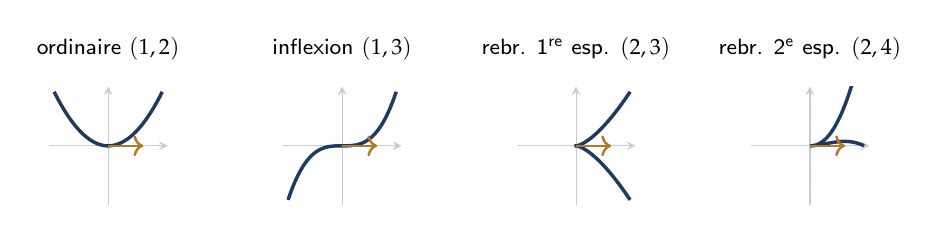
\begin{tikzpicture}
\pgfplotsset{loc/.style={axis lines=middle,axis line style={Filet},width=0.255\linewidth,height=0.255\linewidth,
  xtick=\empty,ytick=\empty,xmin=-1.1,xmax=1.1,ymin=-1.1,ymax=1.1,samples=150,smooth,
  title style={font=\footnotesize\sffamily}}}
\begin{axis}[loc,title={ordinaire $(1,2)$}]
\addplot[arcetude,domain=-1:1]({x},{x^2});\draw[tgte,->](axis cs:0,0)--(axis cs:0.65,0);
\end{axis}
\begin{axis}[loc,xshift=0.245\linewidth,title={inflexion $(1,3)$}]
\addplot[arcetude,domain=-1:1]({x},{x^3});\draw[tgte,->](axis cs:0,0)--(axis cs:0.65,0);
\end{axis}
\begin{axis}[loc,xshift=0.49\linewidth,title={rebr. 1\textsuperscript{re} esp. $(2,3)$}]
\addplot[arcetude,domain=-1:1]({x^2},{x^3});\draw[tgte,->](axis cs:0,0)--(axis cs:0.65,0);
\end{axis}
\begin{axis}[loc,xshift=0.735\linewidth,title={rebr. 2\textsuperscript{e} esp. $(2,4)$}]
\addplot[arcetude,domain=-1:1]({x^2},{x^4+x^5});\draw[tgte,->](axis cs:0,0)--(axis cs:0.65,0);
\end{axis}
\end{tikzpicture}
\caption{Les quatre allures locales (modèles $(t,t^2)$, $(t,t^3)$, $(t^2,t^3)$, $(t^2,t^4+t^5)$) ; la flèche dirige la tangente.}
\label{fig:pq}
\end{figure}

\begin{votrecours}
Le cours décrit ces quatre allures avant le théorème, sur le modèle $(t^p,t^q)$ avec $1\leq p<q$ : en $O$, la corde est
dirigée par $\frac{(t^p,t^q)}{t^p}=(1,t^{q-p})\to(1,0)$, et la parité de $p$ et de $q$ décide si $M(-t)$ est le
symétrique de $M(t)$ par rapport à $(Ox)$, à $(Oy)$ ou à $O$. On y retient deux phrases : au \emph{point ordinaire} et au
\emph{rebroussement de seconde espèce}, la courbe reste du même côté de sa tangente ; au \emph{point d'inflexion} et au
\emph{rebroussement de première espèce}, elle la traverse.

Un point peut aussi être \emph{anguleux} : deux demi-tangentes (limites des cordes pour $t\to t_0^-$ et $t\to t_0^+$)
existent mais ne sont pas colinéaires. Cela n'arrive pas lorsque $f$ est assez régulière pour que $p$ et $q$ existent ;
on le rencontre lorsque $f'$ a des limites différentes à gauche et à droite, par exemple pour $t\mapsto(t,|t|)$ en $0$.
\end{votrecours}

\begin{definition}
Un point $M(t_0)$ d'une courbe de classe $\mathcal C^2$ est \emph{birégulier} si $\big(f'(t_0),f''(t_0)\big)$ est libre,
c'est-à-dire si $\det\big(f'(t_0),f''(t_0)\big)\neq0$ : la vitesse et l'accélération ne sont pas colinéaires.
\end{definition}

Un point birégulier correspond à $p=1$, $q=2$ : c'est un point ordinaire. Le tableau suivant, tiré du cours, résume ce
qu'on peut affirmer sans calcul supplémentaire.
\begin{center}
\renewcommand{\arraystretch}{1.25}\small
\begin{tabular}{l|ccc}
 & point ordinaire & point d'inflexion & rebroussement\\\hline
point régulier ($p=1$) & possible ($q$ pair) & possible ($q$ impair) & impossible\\
point birégulier ($p=1$, $q=2$) & toujours & impossible & impossible
\end{tabular}
\end{center}
Conséquence : \emph{un point d'inflexion régulier n'est pas birégulier}, donc vérifie $\det\big(f'(t_0),f''(t_0)\big)=0$.
Cette condition est nécessaire mais pas suffisante ; la méthode complète de recherche des points d'inflexion figure dans
la boîte à outils (méthode~\ref{meth:inflexion}).

\begin{methode}{Étudier un point par développement limité}\label{meth:dl}
\begin{enumerate}
\item Poser $t=t_0+h$ et développer $x$ et $y$ en puissances de $h$.
\item Regrouper en vecteurs : $f(t_0+h)=f(t_0)+h^p\,\ve a+\dots+h^q\,\ve b+o(h^q)$.
\item S'arrêter au premier vecteur $\ve b$ \emph{non colinéaire} au premier vecteur non nul $\ve a$.
\item Conclure : tangente dirigée par $\ve a$, nature par les parités de $p$ et $q$.
\end{enumerate}
\end{methode}

\begin{attention}
Un vecteur vitesse nul ne signifie ni « pas de tangente », ni « tangente quelconque ». Il signifie seulement que
$f'(t_0)$ ne donne pas la réponse. La tangente existe dès que les entiers $p$ et $q$ existent ; on la trouve sur le
développement limité.
\end{attention}

\marge{Ensemble}
\begin{exemple}[un point stationnaire]\label{ex:cos-sin3}
Étudier le point $M(0)$ de $f(t)=(\cos t,\sin^3t)$.
\chercher
$f'(t)=(-\sin t,3\sin^2t\cos t)$ est nul en $0$. Avec $\cos h=1-\frac{h^2}2+o(h^3)$ et $\sin^3h=h^3+o(h^3)$ :
\[f(h)=(1,0)+h^2\left(-\tfrac12,0\right)+h^3(0,1)+o(h^3).\]
Ainsi $p=2$, $q=3$ : rebroussement de première espèce en $(1,0)$, à tangente horizontale. La courbe arrive vers la
gauche ($\ve a=(-\frac12,0)$ avec $h^2>0$) et se trouve au-dessus de la tangente pour $h>0$, au-dessous pour $h<0$.
\end{exemple}

\begin{exemple}[un terme intermédiaire trompeur]
Pour $f(t)=(t^2+t^3,\ t^4)$ en $0$ : $f(h)=h^2(1,0)+h^3(1,0)+h^4(0,1)$. Le vecteur de $h^3$ est colinéaire au premier : il
ne compte pas. Donc $p=2$, $q=4$ : rebroussement de seconde espèce.
\end{exemple}

\paragraph{C. Position par rapport à la tangente}
\marge{Expliquer}
Le même développement indique de quel côté de la tangente se trouve la courbe. Dans le repère $(M(t_0),\ve a,\ve b)$,
l'ordonnée de $M(t_0+h)$ est équivalente à $h^q$ : la courbe est du côté de $\ve b$ lorsque $h^q>0$. En un point
régulier, cela donne un critère pratique : si $\det\big(f'(t_0),f''(t_0)\big)\neq0$, alors $q=2$, le point est ordinaire,
et la courbe est localement du côté vers lequel pointe $f''(t_0)$.

\begin{exemple}[position et inflexion]
\begin{itemize}
\item Pour $f(t)=(t+t^2,\ t^2+t^3)$ en $0$ : $f(h)=h(1,0)+h^2(1,1)+h^3(0,1)$, donc $p=1$, $q=2$ ; la courbe est du côté de
      $(1,1)$, c'est-à-dire \emph{au-dessus} de sa tangente $(Ox)$.
\item Pour $f(t)=(t,\sin t)$ : $\det(f',f'')=\dt{1&0\\\cos t&-\sin t}=-\sin t$ change de signe en chaque $k\pi$ : la courbe
      change de côté par rapport à ses tangentes, les points $(k\pi,0)$ sont des inflexions.
\end{itemize}
\end{exemple}

\begin{figure}[H]
\centering
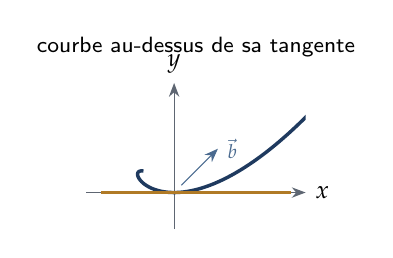
\begin{tikzpicture}
\begin{axis}[courbe,width=0.36\linewidth,xmin=-0.6,xmax=0.9,ymin=-0.25,ymax=0.75,xtick=\empty,ytick=\empty,
  title={\footnotesize\sffamily courbe au-dessus de sa tangente}]
\addplot[arcetude,domain=-0.7:0.6,samples=100]({x+x^2},{x^2+x^3});
\draw[tgte] (axis cs:-0.5,0)--(axis cs:0.8,0);
\draw[-{Stealth[length=5pt]},BleuMoyen] (axis cs:0.05,0.05)--(axis cs:0.3,0.3) node[right,font=\scriptsize]{$\ve b$};
\end{axis}
\end{tikzpicture}\hspace{1cm}
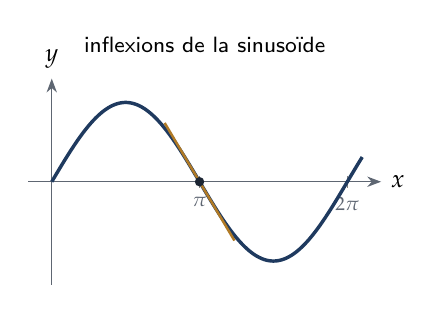
\begin{tikzpicture}
\begin{axis}[courbe,width=0.5\linewidth,xmin=-0.5,xmax=7,ymin=-1.3,ymax=1.3,xtick={3.1416,6.2832},
  xticklabels={$\pi$,$2\pi$},ytick=\empty,title={\footnotesize\sffamily inflexions de la sinusoïde},axis equal image=false,height=4.2cm]
\addplot[arcetude,domain=0:6.6,samples=200]{sin(x)};
\draw[tgte] (axis cs:2.4,0.7416)--(axis cs:3.8832,-0.7416);
\node[pt] at (axis cs:3.1416,0) {};
\end{axis}
\end{tikzpicture}
\caption{À gauche, la courbe reste au-dessus de sa tangente (point ordinaire) ; à droite, elle la traverse (inflexion).}
\end{figure}

\marge{Seul}
\begin{exo}{loc-a}{1}{lecture de $p$ et $q$}
Déterminer la nature du point $M(0)$ pour $f(t)=(t^3,t^5)$, puis pour $f(t)=(t^2+t^3,\ t^3)$.
\end{exo}
\coupdepouce{le développement est déjà écrit : regrouper par puissances de $t$ et chercher le premier vecteur non colinéaire au premier.}

\pointarret{les points singuliers sont acquis. Reprise à l'étape 12 en refaisant au tableau l'exemple de $(\cos t,\sin^3t)$.}

% ---------------------------------------------------------------------
\Etape{12}{20 min}{Branches infinies et asymptotes}{reconnaître toutes les configurations et éviter la confusion entre
direction asymptotique et asymptote.}

\pourquoi Lorsque $t$ tend vers une borne ou une valeur interdite, $|x|$ ou $|y|$ peut devenir infini : la courbe
« part à l'infini ». Le tracé exige de savoir \emph{dans quelle direction} elle part, et si elle s'approche d'une droite.

\marge{Expliquer}
\begin{definition}
Soit $t_0$ une borne de l'intervalle d'étude (ou une valeur interdite) telle que $\|\vv{OM(t)}\|\to+\infty$ lorsque
$t\to t_0$. Une droite $\mathcal D$ est \emph{asymptote} à la courbe en $t_0$ si $d\big(M(t),\mathcal D\big)\to0$ lorsque
$t\to t_0$ : le point s'éloigne à l'infini tout en se rapprochant de la droite fixe $\mathcal D$.
\end{definition}

\rappel{distance d'un point à une droite} Si $\mathcal D:ax+by+c=0$, alors $d\big(M(x_0,y_0),\mathcal D\big)=
\dfrac{|ax_0+by_0+c|}{\sqrt{a^2+b^2}}$. En effet, si $A\in\mathcal D$ et $H$ est le projeté orthogonal de $M$ sur
$\mathcal D$, le vecteur $\ve n=(a,b)$ est normal à $\mathcal D$, donc $\vv{AM}\cdot\ve n=\vv{AH}\cdot\ve n+\vv{HM}\cdot\ve
n=0\pm\|\vv{HM}\|\,\|\ve n\|$ ; et $\vv{AM}\cdot\ve n=ax_0+by_0+c$ car $aA_x+bA_y=-c$.

\emph{Lien avec la méthode.} Pour une droite non verticale $y=\alpha x+\beta$, la distance vaut
$\frac{|y(t)-\alpha x(t)-\beta|}{\sqrt{1+\alpha^2}}$ : elle tend vers $0$ si et seulement si $y(t)-\alpha x(t)\to\beta$. Si
de plus $x$ et $y$ tendent vers l'infini, en divisant par $x(t)$ on obtient $\frac{y(t)}{x(t)}\to\alpha$. D'où les deux
limites à calculer, dans cet ordre : $\alpha=\lim\frac yx$, puis $\beta=\lim(y-\alpha x)$.

\begin{methode}{Classer une branche infinie}\label{meth:branches}
On étudie la limite de $f(t)$ lorsque $t$ tend vers la borne $t_0$.
\begin{enumerate}
\item $x\to\pm\infty$ et $y\to b$ réel : \emph{asymptote horizontale} $y=b$ ; la position se lit sur le signe de $y-b$.
\item $x\to a$ réel et $y\to\pm\infty$ : \emph{asymptote verticale} $x=a$ ; la position se lit sur le signe de $x-a$.
\item $x$ et $y$ infinis : on calcule $\lim y/x$, qui donne la \emph{direction asymptotique}.
\begin{itemize}
\item $y/x\to\pm\infty$ : branche parabolique de direction $(Oy)$ ;
\item $y/x\to0$ : branche parabolique de direction $(Ox)$ ;
\item $y/x\to a\neq0$ : direction $y=ax$ ; on calcule alors $\lim(y-ax)$.
      Si elle vaut $b$ réel, la droite $y=ax+b$ est asymptote ; si elle est infinie, branche parabolique de
      direction $y=ax$ ; si elle n'existe pas, la courbe a une direction asymptotique sans asymptote.
\end{itemize}
\end{enumerate}
\end{methode}

\marge{Questionner}
\question{Pour $t\mapsto(t,\ t+\sqrt t)$, $t\to+\infty$, que vaut $\lim y/x$ ? La droite $y=x$ est-elle asymptote ?}

\marge{Expliquer}
$\frac yx=1+\frac1{\sqrt t}\to1$ : la courbe a la \emph{direction} de $y=x$. Mais $y-x=\sqrt t\to+\infty$ : elle s'éloigne
indéfiniment de toutes les droites de pente $1$. C'est la différence essentielle entre les deux notions : une direction
asymptotique dit vers où la courbe part ; une asymptote est une droite \emph{précise} dont elle se rapproche.

\begin{figure}[H]
\centering
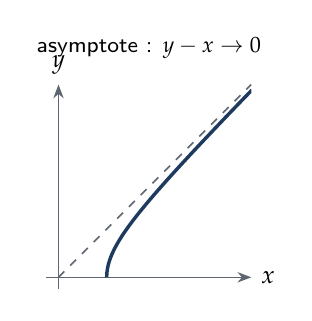
\begin{tikzpicture}
\begin{axis}[courbe,width=0.4\linewidth,xmin=-0.5,xmax=8,ymin=-0.5,ymax=8,xtick=\empty,ytick=\empty,
  title={\footnotesize\sffamily asymptote : $y-x\to0$}]
\addplot[asy,domain=0:8,samples=2]{x};
\addplot[arcetude,domain=1:7.9,samples=100]({x+1/x},{x-1/x});
\end{axis}
\end{tikzpicture}\hspace{0.8cm}
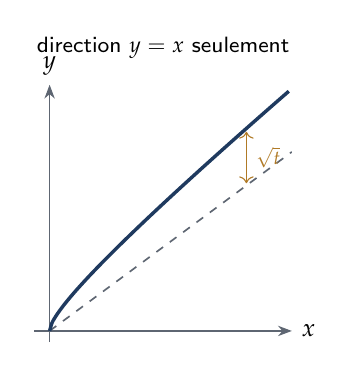
\begin{tikzpicture}
\begin{axis}[courbe,width=0.4\linewidth,xmin=-0.5,xmax=8,ymin=-0.5,ymax=11,xtick=\empty,ytick=\empty,
  title={\footnotesize\sffamily direction $y=x$ seulement},axis equal image=false,height=0.4\linewidth]
\addplot[asy,domain=0:8,samples=2]{x};
\addplot[arcetude,domain=0:7.9,samples=100]({x},{x+sqrt(x)});
\draw[<->,Ocre] (axis cs:6.5,6.6)--(axis cs:6.5,8.9) node[midway,right,font=\scriptsize]{$\sqrt t$};
\end{axis}
\end{tikzpicture}
\caption{À gauche, $(t+\frac1t,\,t-\frac1t)$ s'approche de la droite $y=x$ ; à droite, $(t,\,t+\sqrt t)$ a la même direction
mais l'écart grandit indéfiniment.}
\end{figure}

\begin{astuce}
On ne calcule pas toutes les limites : on commence par les \emph{limites de $x$ et $y$}, qui disent immédiatement dans
quel cas l'on se trouve. Pour le calcul de $y-ax$ et de la position, un \emph{développement asymptotique} donne les deux
d'un coup : si $y-ax=b+c(t)$ avec $c(t)\to0$, le signe de $c(t)$ donne la position.
\end{astuce}

\marge{Ensemble}
\begin{exemple}[asymptote oblique et position]
Étudier la branche infinie de $f(t)=\left(\dfrac{t}{t-1},\dfrac{t^2}{t-1}\right)$ lorsque $t\to1$.
\chercher
$x$ et $y$ tendent vers l'infini ; $\frac yx=t\to1$ ; $y-x=\frac{t^2-t}{t-1}=t\to1$. La droite $y=x+1$ est asymptote.
Comme $y-x-1=t-1$, la courbe est au-dessus de l'asymptote quand $t\to1^+$ (côté $x\to+\infty$), au-dessous quand $t\to1^-$
(côté $x\to-\infty$). Cette courbe est étudiée en entier à l'exemple~\ref{ex:g4}.
\end{exemple}

\begin{attention}
On n'oublie pas les \emph{valeurs interdites} du paramètre : ici, la branche intéressante n'est pas en $\pm\infty$ mais en
$t=1$. Et l'on n'affirme pas l'existence d'une asymptote tant que $\lim(y-ax)$ n'a pas été calculée.
\end{attention}

\marge{Seul}
\begin{exo}{br-d}{2}{direction asymptotique ou asymptote ?}
\begin{enumerate}
\item Étudier la branche infinie de $f(t)=(t,\ t+\ln t)$ lorsque $t\to+\infty$.
\item Même question pour $g(t)=\left(t+\frac1t,\ t+2+\frac1{t^2}\right)$ ; préciser la position de la courbe.
\end{enumerate}
\end{exo}
\coupdepouce{calculer successivement $\lim x$, $\lim y$, $\lim\frac yx$, puis $\lim(y-x)$ ; ne conclure qu'à la fin.}

\pointarret{tous les outils sont en place. Reprise à l'étape 13 ; l'étape 14 peut faire l'objet d'une séance à part entière, en y ajoutant un exemple de la galerie.}

% ---------------------------------------------------------------------
\Etape{13}{10 min}{Passer des calculs au dessin}{savoir quoi placer, dans quel ordre, et avec quelle précision.}

\pourquoi Les calculs fournissent des renseignements dispersés : des points, des directions, des limites. Un tracé juste
les \emph{superpose} dans un ordre précis ; un tracé faux les relie au hasard.

\marge{Expliquer}
\begin{methode}{Construire le tracé}\label{meth:trace}
\begin{enumerate}
\item Tracer les axes à une échelle adaptée aux valeurs remarquables du tableau.
\item Tracer les asymptotes en pointillés.
\item Placer les points remarquables (tangentes horizontales, verticales, points singuliers, intersections avec les
      axes) et dessiner à chacun un \emph{petit segment de tangente}.
\item Relier ces points en suivant le tableau : entre deux lignes du tableau, $x$ et $y$ sont monotones, donc l'arc va
      toujours dans la même « direction cardinale » (par exemple vers la droite et vers le bas si $x\nearrow$ et
      $y\searrow$).
\item Dessiner les branches infinies en les faisant approcher de leurs asymptotes du bon côté.
\item Compléter par les symétries, dans l'ordre inverse des réductions.
\item Indiquer le sens de parcours par quelques flèches.
\end{enumerate}
\end{methode}

\begin{reflexe}
Le tableau de variations conjoint se lit comme un guide de tracé : chaque colonne donne un point, chaque intervalle une
direction de déplacement. Le signe de $(x',y')$ suffit : $(+,+)$ vers le haut à droite, $(+,-)$ vers le bas à droite,
$(-,+)$ vers le haut à gauche, $(-,-)$ vers le bas à gauche.
\end{reflexe}

% ---------------------------------------------------------------------
\Etape{14}{35 min}{Une étude complète, construite pas à pas}{appliquer tout le plan sur une courbe qui réunit
symétrie, point singulier, tangente horizontale, asymptote et branche parabolique.}

\marge{Ensemble}
\begin{exemple}\label{ex:seance2}
Étudier et tracer la courbe $f(t)=\left(t^2,\ \dfrac{t^3}{t^2-1}\right)$.
\end{exemple}

\etape{1. Ensemble de définition} $\mathcal D=\R\setminus\{-1,1\}$. Les valeurs interdites $\pm1$ annoncent des branches
infinies.

\etape{2. Réduction} $x$ est paire et $y$ impaire : $M(-t)$ est le symétrique de $M(t)$ par rapport à $(Ox)$. On étudie sur
$[0,1[\,\cup\,]1,+\infty[$, puis on complète par la symétrie d'axe $(Ox)$.

\etape{3. Dérivées} $x'(t)=2t$ et, après simplification,
\[y'(t)=\frac{3t^2(t^2-1)-2t\cdot t^3}{(t^2-1)^2}=\frac{t^2(t^2-3)}{(t^2-1)^2}.\]
\emph{Interprétation} : $x'$ et $y'$ s'annulent ensemble en $t=0$ (point singulier) ; $y'$ s'annule seule en $t=\sqrt3$
(tangente horizontale) ; $x$ croît toujours pour $t>0$.

\etape{4. Tableau conjoint}
\begin{center}
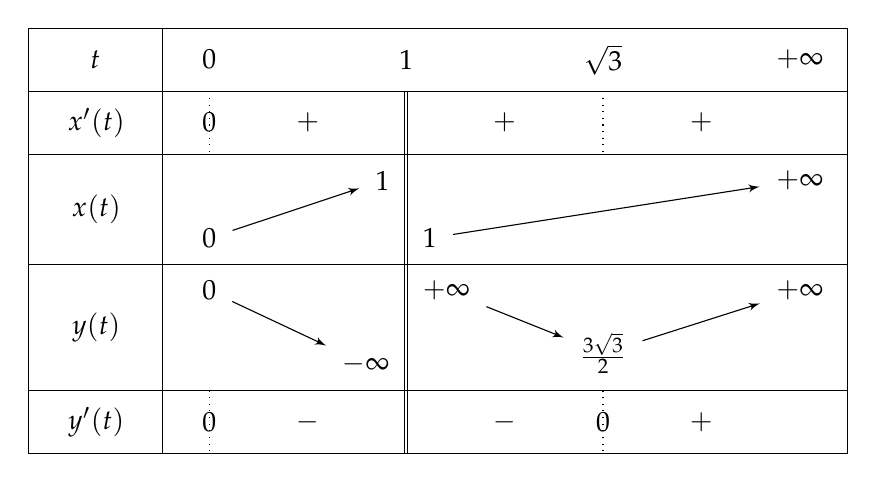
\begin{tikzpicture}
\tkzTabInit[lgt=1.7,espcl=2.5,deltacl=0.6]{$t$/0.8,$x'(t)$/0.8,$x(t)$/1.4,$y(t)$/1.6,$y'(t)$/0.8}{$0$,$1$,$\sqrt3$,$+\infty$}
\tkzTabLine{z,+,d,+,t,+,}
\tkzTabVar{-/$0$,+D-/$1$/$1$,R/,+/$+\infty$}
\tkzTabVar{+/$0$,-D+/$-\infty$/$+\infty$,-/$\frac{3\sqrt3}2$,+/$+\infty$}
\tkzTabLine{z,-,d,-,z,+,}
\end{tikzpicture}
\end{center}
\emph{Lecture} : sur $]0,1[$, $(x',y')=(+,-)$, la courbe va vers la droite et vers le bas ; sur $]1,\sqrt3[$, aussi, mais
elle vient du haut ; sur $]\sqrt3,+\infty[$, vers la droite et vers le haut.

\etape{5. Point singulier $O$} Pour $t$ voisin de $0$, $\frac{t^3}{t^2-1}=-t^3(1+t^2+\dots)=-t^3+o(t^3)$, d'où
\[f(t)=t^2(1,0)+t^3(0,-1)+o(t^3).\]
$p=2$, $q=3$ : rebroussement de première espèce, tangente horizontale. La courbe arrive de la droite ($x=t^2>0$) et,
pour $t>0$, se trouve sous l'axe ($y\sim-t^3$).

\etape{6. Tangente horizontale} En $t=\sqrt3$ : $M(\sqrt3)=\left(3,\frac{3\sqrt3}2\right)\approx(3\,;\,2{,}60)$.

\etape{7. Branches infinies}
\begin{itemize}
\item $t\to1$ : $x\to1$, $y\to\mp\infty$ (selon le côté) : \emph{asymptote verticale} $x=1$. Pour $t\to1^-$, $x=t^2<1$ : la
      courbe est à gauche de l'asymptote et descend ; pour $t\to1^+$, elle est à droite et vient du haut.
\item $t\to+\infty$ : $x\to+\infty$, $y\sim t\to+\infty$, $\frac yx=\frac{t}{t^2-1}\to0$ : \emph{branche parabolique de
      direction $(Ox)$}. La courbe part vers la droite en montant de plus en plus lentement, comme $y\approx\sqrt x$.
\end{itemize}

\etape{8. Construction} La figure~\ref{fig:construction} montre les trois temps du tracé : les éléments fixes (asymptote,
points, tangentes), puis l'arc d'étude guidé par le tableau, enfin la symétrie.

\begin{figure}[H]
\centering
\pgfplotsset{etape/.style={courbe,width=0.36\linewidth,height=0.5\linewidth,axis equal image=false,
  xlabel={},ylabel={},xmin=-0.4,xmax=4.6,ymin=-5.2,ymax=5.2,xtick={1,3},ytick={-2.6,2.6},yticklabels={},
  title style={font=\footnotesize\sffamily,yshift=2pt},
  unbounded coords=jump,restrict y to domain=-12:12}}
\begin{tikzpicture}
\begin{axis}[etape,title={1. éléments fixes}]
\addplot[asy,samples=2] coordinates {(1,-5.2) (1,5.2)};
\draw[tgte] (axis cs:2.4,2.598)--(axis cs:3.6,2.598);
\draw[tgte] (axis cs:0,0)--(axis cs:0.7,0);
\node[pt] at (axis cs:0,0) {}; \node[pt] at (axis cs:3,2.598) {};
\node[font=\scriptsize,anchor=south] at (axis cs:3,2.7) {$M(\sqrt3)$};
\node[font=\scriptsize,anchor=north west] at (axis cs:0.05,-0.1) {$O$};
\draw[-{Stealth[length=4pt]},BleuMoyen] (axis cs:0.8,-3.0)--(axis cs:0.9,-4.4);
\draw[-{Stealth[length=4pt]},BleuMoyen] (axis cs:1.15,4.6)--(axis cs:1.3,3.4);
\draw[-{Stealth[length=4pt]},BleuMoyen] (axis cs:3.7,3.3)--(axis cs:4.5,3.7);
\end{axis}
\end{tikzpicture}%
\begin{tikzpicture}
\begin{axis}[etape,title={2. arc d'étude ($t\geq0$)}]
\addplot[asy,samples=2] coordinates {(1,-5.2) (1,5.2)};
\addplot[arcetude,domain=0:0.985,samples=250]({x^2},{x^3/(x^2-1)});
\addplot[arcetude,domain=1.02:2.15,samples=250]({x^2},{x^3/(x^2-1)});
\draw[tgte] (axis cs:2.4,2.598)--(axis cs:3.6,2.598);
\node[pt] at (axis cs:0,0) {}; \node[pt] at (axis cs:3,2.598) {};
\end{axis}
\end{tikzpicture}%
\begin{tikzpicture}
\begin{axis}[etape,title={3. symétrie d'axe $(Ox)$}]
\addplot[asy,samples=2] coordinates {(1,-5.2) (1,5.2)};
\addplot[reste,domain=0:0.985,samples=250]({x^2},{-x^3/(x^2-1)});
\addplot[reste,domain=1.02:2.15,samples=250]({x^2},{-x^3/(x^2-1)});
\addplot[arcetude,domain=0:0.985,samples=250]({x^2},{x^3/(x^2-1)});
\addplot[arcetude,domain=1.02:2.15,samples=250]({x^2},{x^3/(x^2-1)});
\node[pt] at (axis cs:0,0) {};
\end{axis}
\end{tikzpicture}
\caption{Construction du tracé de $\left(t^2,\frac{t^3}{t^2-1}\right)$ : asymptote $x=1$, rebroussement en $O$, tangente
horizontale en $\left(3,\frac{3\sqrt3}2\right)$, branches paraboliques de direction $(Ox)$.}\label{fig:construction}
\end{figure}

\etape{9. Vérification} On contrôle la cohérence : le point $M(2)=\left(4,\frac83\right)$ est bien sur l'arc qui remonte après
le minimum ; la courbe ne coupe l'axe $(Ox)$ qu'en $O$, puisque $y=0$ impose $t=0$ ; près de $O$, les deux arcs symétriques
forment bien une pointe tournée vers la gauche.

\begin{enpratique}
Cette étude contient toutes les difficultés classiques. Retenir l'enchaînement : valeurs interdites $\Rightarrow$
branches infinies ; parités $\Rightarrow$ intervalle réduit ; $x'$ et $y'$ factorisées $\Rightarrow$ points singuliers et
tangentes remarquables ; tableau $\Rightarrow$ directions de déplacement ; développement limité $\Rightarrow$ allure en $O$.
\end{enpratique}

\marge{Seul}
\begin{exo}{tp1}{2}{point singulier, allure locale, sens de parcours}
Soit $f(t)=(t^2+t^3,\ t^2-t^3)$. Montrer que $M(0)$ est un point singulier, déterminer la tangente et la nature de ce
point, puis dessiner l'allure de la courbe au voisinage de $O$ en indiquant le sens de parcours.
\end{exo}
\coupdepouce{le développement est exact ; pour le sens de parcours, regarder comment varie $t^2$ quand $t$ passe de $-0{,}5$ à $0{,}5$.}

\subsection*{Bilan de la séance 2}
\addcontentsline{toc}{subsection}{Bilan de la séance 2 {\color{Gris}(5 min)}}

\marge{Questionner}
\begin{enumerate}
\item Que faire lorsque $f'(t_0)=\ve0$ ? \hfill{\small\color{Gris}(développement limité, entiers $p$ et $q$)}
\item À quoi reconnaît-on un rebroussement ? \hfill{\small\color{Gris}($p$ pair)}
\item $y/x\to2$ : y a-t-il une asymptote ? \hfill{\small\color{Gris}(seulement si $y-2x$ a une limite finie)}
\item Comment le tableau de variations guide-t-il le tracé ? \hfill{\small\color{Gris}(signes de $x'$, $y'$ = direction)}
\end{enumerate}
Pour le travail personnel : relire la méthode commentée (section~\ref{sec:methode-commentee}), étudier deux exemples de la
galerie, puis chercher les exercices dans l'ordre.

% =====================================================================
%   CHAPITRE 5 (SUITE) — RÉFÉRENCE MÉTHODOLOGIQUE POUR LE TRACÉ
% =====================================================================
\clearpage
\subsection*{Deuxième partie --- référence pour le travail personnel}
\addcontentsline{toc}{subsection}{\textit{Deuxième partie : référence pour le travail personnel}}

Cette partie se consulte après la séance 2, et pendant les exercices. Elle reprend la démarche de façon détaillée, puis
la montre à l'œuvre sur six courbes choisies pour couvrir les configurations classiques.

% ---------------------------------------------------------------------
\subsection{La méthode commentée}\label{sec:methode-commentee}

Chaque étape est présentée avec sa raison d'être, les calculs à faire, l'interprétation géométrique des résultats, les
pièges, et les cas où l'on peut l'alléger.

\paragraph{1. Ensemble de définition}
\emph{Pourquoi} : les valeurs exclues du paramètre sont les endroits où la courbe peut partir à l'infini.
\emph{Comment} : intersection des ensembles de définition de $x$ et $y$ ; noter explicitement les valeurs interdites et les
bornes. \emph{Piège} : oublier une valeur interdite, et donc une branche infinie.

\paragraph{2. Symétries et périodicité}
\emph{Pourquoi} : chaque symétrie divise le travail par deux. \emph{Comment} : comparer $f(-t)$, $f(t+T)$, $f(\pi-t)$,
$f(1/t)$ à $f(t)$ ; traduire géométriquement (tableau du chapitre 2). \emph{Piège} : oublier de vérifier que la
transformation envoie la partie étudiée sur la partie manquante. \emph{Simplification} : si $x$ et $y$ n'ont aucune parité
évidente, on ne s'attarde pas.

\paragraph{3. Intervalle d'étude}
\emph{Pourquoi} : on ne calcule que sur ce qui est nécessaire. \emph{Comment} : réduire successivement, noter l'ordre des
réductions pour les inverser au moment du tracé.

\paragraph{4. Limites aux bornes}
\emph{Pourquoi} : elles fixent les extrémités de chaque arc et signalent les branches infinies. \emph{Comment} : calculer
$\lim x$ et $\lim y$ en chaque borne de chaque intervalle, à gauche et à droite des valeurs interdites. \emph{Interprétation}
: une limite finie donne un point (atteint ou non) ; une limite infinie annonce une branche à étudier à l'étape 9.

\paragraph{5. Dérivées}
\emph{Pourquoi} : elles donnent la direction du mouvement. \emph{Comment} : calculer $x'$ et $y'$ et les \emph{factoriser}
complètement. \emph{Interprétation} : les zéros communs sont les points singuliers ; un zéro de $y'$ seul donne une
tangente horizontale, un zéro de $x'$ seul une tangente verticale. \emph{Piège} : développer $x'$ au lieu de le factoriser,
ce qui rend l'étude du signe difficile.

\paragraph{6. Variations}
\emph{Pourquoi} : sur chaque intervalle où $x'$ et $y'$ gardent un signe, l'arc se déplace dans une direction fixe.
\emph{Comment} : un seul tableau conjoint, lignes $t$, $x'$, $x$, $y$, $y'$, avec les valeurs aux points remarquables et les
limites. \emph{Interprétation} : voir le réflexe de l'étape 13.

\paragraph{7. Points réguliers et singuliers}
\emph{Pourquoi} : en un point régulier, la tangente est connue ; en un point singulier, elle doit être cherchée.
\emph{Comment} : $f'(t_0)=\ve0$ si et seulement si $x'(t_0)=y'(t_0)=0$. \emph{Piège} : affirmer « tangente verticale » parce
que $x'(t_0)=0$, sans vérifier $y'(t_0)\neq0$.

\paragraph{8. Tangentes et position}
\emph{Comment} : en un point régulier, tangente dirigée par $f'(t_0)$ ; en un point singulier, développement limité
(méthode~\ref{meth:dl}). La position est donnée par le terme en $h^q$. \emph{Simplification} : on ne fait de développement
limité qu'aux points singuliers et, si l'énoncé le demande, aux points d'inflexion possibles.

\paragraph{9. Branches infinies}
\emph{Comment} : méthode~\ref{meth:branches}. \emph{Piège} : conclure à une asymptote dès que $y/x\to a$.
\emph{Simplification} : si $x$ tend vers une limite finie, ou $y$ vers une limite finie, la branche est immédiatement classée
(asymptote verticale ou horizontale) : inutile de calculer $y/x$.

\paragraph{10. Positions relatives}
\emph{Pourquoi} : une asymptote mal placée par rapport à la courbe fausse tout le tracé. \emph{Comment} : signe de $y-ax-b$
(asymptote oblique), de $x-a$ (verticale), de $y-b$ (horizontale), en distinguant les deux côtés de la borne.

\paragraph{11. Tracé}
\emph{Comment} : méthode~\ref{meth:trace}. \emph{Vérification} : calculer un point non remarquable et vérifier qu'il tombe sur
le tracé ; vérifier que le tracé respecte toutes les lignes du tableau.

% ---------------------------------------------------------------------
\subsection{Boîte à outils du tracé}

\paragraph{Tracer une droite donnée par un point et un vecteur} À partir du point $A$, on reporte le vecteur $\ve u$ (ou un
multiple commode) pour obtenir un second point $B=A+\lambda\ve u$, puis on trace $(AB)$. Pour une pente $\frac{\beta}{\alpha}$, on
avance de $\alpha$ et l'on monte de $\beta$.

\paragraph{Tracer une tangente} On ne trace qu'un \emph{petit segment} centré sur le point, assez long pour guider la main.
En un point de rebroussement, on trace la demi-tangente du côté où arrive la courbe.

\paragraph{Tracer une asymptote} En pointillés, sur toute la fenêtre. La branche s'en approche sans la couper au voisinage de
l'infini, \emph{du côté donné par la position relative}.

\paragraph{Tracer une branche parabolique} De direction $(Ox)$ : la courbe s'aplatit (comme $\sqrt x$) ; de direction $(Oy)$ :
elle se redresse (comme $x^2$) ; de direction $y=ax$ : elle s'éloigne indéfiniment de toutes les droites de pente $a$.

\begin{figure}[H]
\centering
\pgfplotsset{br/.style={axis lines=middle,axis line style={Filet},width=0.255\linewidth,height=0.255\linewidth,
  xtick=\empty,ytick=\empty,xmin=-0.5,xmax=4.5,ymin=-0.5,ymax=4.5,samples=100,smooth,title style={font=\footnotesize\sffamily}}}
\begin{tikzpicture}
\begin{axis}[br,title={asymptote horizontale}]
\addplot[asy,samples=2,domain=0:4.5]{1};\addplot[arcetude,domain=0.4:4.4]{1+1/(x+0.2)^1.5};
\end{axis}
\begin{axis}[br,xshift=0.245\linewidth,title={asymptote verticale}]
\addplot[asy,samples=2] coordinates {(1,0) (1,4.5)};\addplot[arcetude,domain=1.15:4.4]{1/(x-1)^0.8};
\end{axis}
\begin{axis}[br,xshift=0.49\linewidth,title={branche parab. $(Ox)$}]
\addplot[arcetude,domain=0:4.4]{1.5*sqrt(x)};
\end{axis}
\begin{axis}[br,xshift=0.735\linewidth,title={branche parab. $(Oy)$}]
\addplot[arcetude,domain=0:2.1]{x^2};
\end{axis}
\end{tikzpicture}
\caption{Les quatre allures de branche infinie les plus fréquentes.}
\end{figure}

\paragraph{Tracer une courbe symétrique} On trace d'abord soigneusement l'arc d'étude, puis on le reporte par chaque
symétrie, dans l'ordre inverse des réductions. Les points situés sur un axe de symétrie sont des points de raccord : la
tangente y est perpendiculaire à l'axe, ou bien le point est singulier.

\paragraph{Points singuliers multiples, intersections} Si la courbe a plusieurs points singuliers, chacun est étudié par son
propre développement limité. Pour les points multiples, on résout $f(t)=f(s)$ avec $t\neq s$ ; une symétrie aide souvent
(par exemple, un point double sur l'axe de symétrie $(Oy)$ vérifie $x(t)=0$).

\paragraph{Sens de parcours} Il est donné par le signe de $(x',y')$ ; on le matérialise par deux ou trois flèches. Il permet de
contrôler qu'on relie les arcs dans le bon ordre.

\paragraph{Points à placer en priorité} Dans l'ordre : points singuliers, points à tangente horizontale ou verticale, points
multiples, intersections avec les axes (résoudre $x(t)=0$ et $y(t)=0$), points limites des branches.

\paragraph{Où être précis} Près des points singuliers (la forme de la pointe), près des points multiples (l'angle entre les
tangentes) et près des asymptotes (le côté par lequel la courbe arrive). Ailleurs, une allure fidèle aux variations suffit.

% ---------------------------------------------------------------------

\subsubsection{Compléments : les outils du TD et du devoir surveillé}\label{sec:outils-td}

Les feuilles de TD et le devoir surveillé de la classe demandent quelques outils supplémentaires, qui ne font pas partie
de l'étude « standard » mais reviennent dans presque tous les problèmes. Chacun est accompagné d'un exercice du
chapitre~\ref{sec:entrainement}.

\begin{methode}{Rechercher les points d'inflexion}\label{meth:inflexion}
\begin{enumerate}
\item \emph{Candidats.} En un point régulier, une inflexion impose $\det\big(f'(t),f''(t)\big)=0$ (un point birégulier
      est ordinaire). On résout cette équation, en se limitant à l'intervalle d'étude.
\item \emph{Simplifier avant de dériver deux fois.} Si $f'(t)=\lambda(t)\,\ve g(t)$ avec $\lambda$ scalaire non nul, alors
      $f''=\lambda'\ve g+\lambda\ve g'$ et
      \[\det(f',f'')=\lambda^2\det(\ve g,\ve g') :\]
      on étudie le signe de $\det(\ve g,\ve g')$, beaucoup plus simple. Avec des fonctions trigonométriques, on
      \emph{linéarise} ($\sin a\sin b=\frac12[\cos(a-b)-\cos(a+b)]$, etc.).
\item \emph{Confirmer.} Si le déterminant \emph{change de signe} en $t_0$, c'est une inflexion ; s'il garde un signe
      (racine double), c'est un point ordinaire. Variante du cours : vérifier que $\big(f'(t_0),f'''(t_0)\big)$ est libre,
      ce qui donne $q=3$, impair.
\end{enumerate}
\end{methode}

\emph{Pourquoi le changement de signe suffit.} Au voisinage d'un point régulier, Taylor--Young montre que
$\det\big(f'(t_0+h),f''(t_0+h)\big)$ est équivalent à $C\,h^{q-2}$, avec
$C=\frac{1}{(q-2)!}\det\big(f'(t_0),f^{(q)}(t_0)\big)\neq0$ : il change de signe si et seulement si $q$ est impair.

\begin{astuce}
La pente de la tangente, $p(t)=\frac{y'(t)}{x'(t)}$, a pour dérivée $p'(t)=\frac{\det(f'(t),f''(t))}{x'(t)^2}$. Aux points
d'inflexion où la tangente n'est pas verticale, la pente est donc \emph{extrémale} (localement). C'est pourquoi, dans un
devoir, la question « trouver le point où la tangente a pour pente $m$ » donne souvent une racine double en un point
d'inflexion : l'équation $p(t)=m$ y a une solution double.
\end{astuce}

\begin{methode}{Position globale par rapport à une droite}\label{meth:posglob}
Soit $\mathcal D:ax+by+c=0$. On pose $\varphi(t)=a\,x(t)+b\,y(t)+c$.
\begin{enumerate}
\item Les racines de $\varphi$ donnent les points communs à la courbe et à $\mathcal D$.
\item Le signe de $\varphi(t)$ indique de quel côté de $\mathcal D$ se trouve $M(t)$ : le demi-plan $ax+by+c>0$ ou
      l'autre.
\item On étudie $\varphi$ comme une fonction numérique : dérivée factorisée, tableau de variations, signe.
\end{enumerate}
Si $\mathcal D$ est la tangente en $M(t_0)$, on sait d'avance que $\varphi(t_0)=0$ et $\varphi'(t_0)=0$ : $t_0$ est racine
au moins double, ce qui aide à factoriser $\varphi'$.
\end{methode}

\paragraph{Intersection d'une courbe et d'une droite} On substitue le paramétrage dans l'équation de la droite. Lorsque
l'équation obtenue fait intervenir $\cos t$ et $\sin t$, on exprime tout en fonction de $X=\cos t$ (au besoin en élevant au
carré, ce qui oblige à vérifier les signes à la fin). Une tangente donne une racine au moins double ; un point double
situé sur la droite donne une racine de plus. Exemple complet : la galerie, exemple~\ref{ex:g7}.

\paragraph{Tangente de pente donnée, tangente parallèle à une direction} La tangente en un point régulier est parallèle
au vecteur $\ve w=(\alpha,\beta)$ si et seulement si $\det\big(f'(t),\ve w\big)=0$ ; pour une pente $m$, on prend
$\ve w=(1,m)$, soit $y'(t)=m\,x'(t)$. On n'oublie pas de vérifier que les solutions sont des points réguliers.

\paragraph{Point limite et prolongement} Si $M(t)$ tend vers un point $A$ \emph{fini} lorsque $t$ tend vers une borne ou
une valeur interdite, il n'y a pas de branche infinie : la courbe « se termine » en $A$, que l'on place sur le dessin
(cercle vide s'il n'est pas atteint). La direction d'arrivée est la limite de la direction de la corde $\vv{AM(t)}$ :
on calcule $\lim\frac{y(t)-y_A}{x(t)-x_A}$. Si elle vaut $m$, la courbe arrive en $A$ tangentiellement à la droite de pente
$m$ ; si elle est infinie, tangentiellement à la verticale.

\begin{horsprogramme}\phantomsection\label{hp:courbe-asymptote}
\textbf{Courbe asymptote.} Une courbe $\Gamma$ (une parabole, une cubique, une exponentielle\dots) est asymptote à la
courbe paramétrée en $t_0$ si la distance de $M(t)$ à $\Gamma$ tend vers $0$. En pratique, on exhibe un point
$P_t\in\Gamma$ tel que $\|\vv{M(t)P_t}\|\to0$ :
\begin{itemize}
\item si $\Gamma:y=g(x)$, on essaie $P_t=\big(x(t),g(x(t))\big)$, de même abscisse : il suffit que $y(t)-g(x(t))\to0$ ;
\item si $\Gamma$ est très pentue (exponentielle), on essaie plutôt $P_t$ de même \emph{ordonnée} : avec
      $\Gamma:y=e^x+c$, $P_t=\big(\ln(y(t)-c),\,y(t)\big)$, et il suffit que $x(t)-\ln\big(y(t)-c\big)\to0$.
\end{itemize}
Le premier cas se rencontre avec les branches paraboliques : on précise alors la branche par une parabole ou une cubique
asymptote. Attention, la notion est moins rigide que pour une droite : si la distance horizontale à $y=e^x+c$ tend vers
$0$, elle tend aussi vers $0$ pour \emph{toute} autre constante $c'$, car $\ln(y-c)-\ln(y-c')\to0$. Seule la distance
verticale distingue alors une constante privilégiée (exercice~\ref{e:ds-pb}).
\end{horsprogramme}

\begin{astuce}
Pour factoriser une somme ou une différence de cosinus, on passe par les exponentielles et l'\emph{angle moitié} :
\[e^{ia}-e^{ib}=e^{i\frac{a+b}2}\left(e^{i\frac{a-b}2}-e^{-i\frac{a-b}2}\right)=2i\sin\tfrac{a-b}2\,e^{i\frac{a+b}2},\]
d'où, en prenant la partie réelle, $\cos a-\cos b=-2\sin\frac{a-b}2\sin\frac{a+b}2$. Par exemple
$\cos t-\cos2t=\mathrm{Re}\big(e^{it}-e^{2it}\big)=2\sin\frac t2\sin\frac{3t}2$, et de même
$\cos t+\cos2t=2\cos\frac t2\cos\frac{3t}2$. On lit alors directement les zéros et le signe.
\end{astuce}

\paragraph{Lieu géométrique} Lorsqu'un point est défini par une construction (un point d'une échelle qui glisse, un point
construit à partir d'un cercle et d'une droite), on choisit un paramètre naturel (un angle, la pente d'une droite issue
d'un point fixe), on exprime les coordonnées du point en fonction de ce paramètre, et l'on étudie la courbe obtenue.

\begin{horsprogramme}
\textbf{Coordonnées polaires.} Certaines courbes s'écrivent plus simplement en polaire : $M=O+r\,\ve u_\theta$ avec
$\ve u_\theta=(\cos\theta,\sin\theta)$, la courbe étant donnée par une relation entre $r$ et $\theta$. Par exemple, la
cardioïde $\big((1+\cos t)\cos t,(1+\cos t)\sin t\big)$ est la courbe $r=1+\cos\theta$, et la lemniscate de Bernoulli vérifie
$r^2=\cos2\theta$. Pour passer d'une équation cartésienne à une équation polaire, on remplace $x$ par $r\cos\theta$ et $y$
par $r\sin\theta$. L'étude des courbes polaires est hors programme en PT ; seule cette traduction est demandée en TD
(exercice~\ref{e:lemni}).
\end{horsprogramme}

\subsection{Galerie d'exemples entièrement étudiés}

Les sept exemples suivants sont classés par difficulté croissante. Chacun met en avant une configuration particulière ;
ensemble, ils couvrent toutes les situations du programme.

% ...........................................................
\subsubsection{Une courbe symétrique à point double}

\begin{exemple}\label{ex:g1}
Étudier et tracer $f(t)=(t^3-3t,\ t^2)$.
\end{exemple}

\etape{Premières observations} $f$ est polynomiale. $x$ est impaire, $y$ paire : $M(-t)$ est le symétrique de $M(t)$ par
rapport à $(Oy)$. Étude sur $[0,+\infty[$.

\etape{Dérivées} $x'(t)=3(t-1)(t+1)$, $y'(t)=2t$ : jamais nulles ensemble, la courbe est régulière. Tangente horizontale en
$t=0$ (point $O$, car $x'(0)=-3\neq0$), verticale en $t=1$ (point $A(-2,1)$, car $y'(1)=2\neq0$).

\etape{Tableau}
\begin{center}
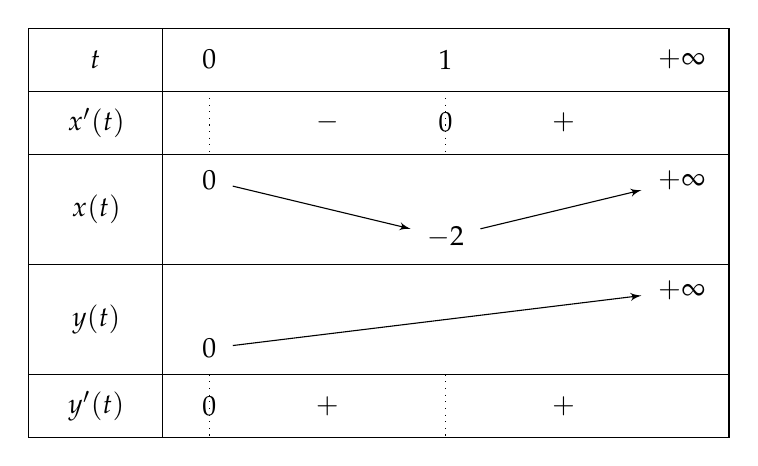
\begin{tikzpicture}
\tkzTabInit[lgt=1.7,espcl=3,deltacl=0.6]{$t$/0.8,$x'(t)$/0.8,$x(t)$/1.4,$y(t)$/1.4,$y'(t)$/0.8}{$0$,$1$,$+\infty$}
\tkzTabLine{t,-,z,+,}
\tkzTabVar{+/$0$,-/$-2$,+/$+\infty$}
\tkzTabVar{-/$0$,R/,+/$+\infty$}
\tkzTabLine{z,+,t,+,}
\end{tikzpicture}
\end{center}
Sur $]0,1[$, $(x',y')=(-,+)$ : vers la gauche et vers le haut ; sur $]1,+\infty[$, $(+,+)$ : vers la droite et vers le haut.

\etape{Point double} Par symétrie, un point double se trouve sur l'axe $(Oy)$ : $x(t)=0\iff t=0$ ou $t^2=3$. Le point
$D(0,3)$ est atteint pour $t=\sqrt3$ et $t=-\sqrt3$. Les tangentes y sont dirigées par $f'(\pm\sqrt3)=(6,\pm2\sqrt3)$, de pentes
$\pm\frac1{\sqrt3}$.

\etape{Branche infinie} $t\to+\infty$ : $\frac yx=\frac{t^2}{t^3-3t}\to0$ : branche parabolique de direction $(Ox)$.

\etape{Tracé et cohérence} On place $O$, $A$, $D$ et leurs tangentes, on relie selon le tableau, puis on reporte par symétrie
(figure~\ref{fig:g1}). La boucle formée entre $t=-\sqrt3$ et $t=\sqrt3$ passe par $O$ et par les deux points $(\pm2,1)$ à
tangente verticale ; c'est cohérent avec $x$ décroissant puis croissant sur $[0,\sqrt3]$.

\begin{figure}[H]
\centering
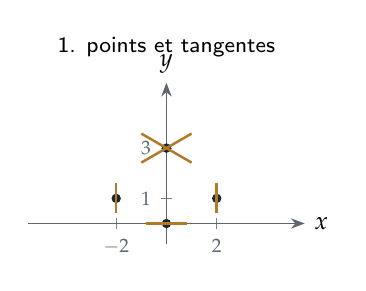
\begin{tikzpicture}
\begin{axis}[courbe,width=0.42\linewidth,xmin=-5.5,xmax=5.5,ymin=-0.8,ymax=5.6,xtick={-2,2},ytick={1,3},
  title={\footnotesize\sffamily 1. points et tangentes}]
\node[pt] at (axis cs:0,0) {}; \draw[tgte] (axis cs:-0.8,0)--(axis cs:0.8,0);
\node[pt] at (axis cs:-2,1) {}; \draw[tgte] (axis cs:-2,0.4)--(axis cs:-2,1.6);
\node[pt] at (axis cs:2,1) {}; \draw[tgte] (axis cs:2,0.4)--(axis cs:2,1.6);
\node[pt] at (axis cs:0,3) {};
\draw[tgte] (axis cs:-1,2.423)--(axis cs:1,3.577); \draw[tgte] (axis cs:-1,3.577)--(axis cs:1,2.423);
\end{axis}
\end{tikzpicture}\hspace{0.5cm}
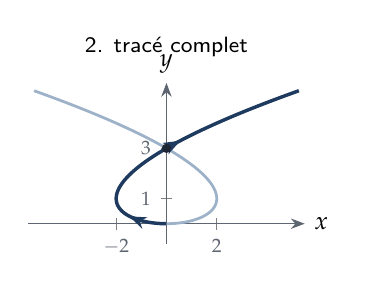
\begin{tikzpicture}
\begin{axis}[courbe,width=0.42\linewidth,xmin=-5.5,xmax=5.5,ymin=-0.8,ymax=5.6,xtick={-2,2},ytick={1,3},
  title={\footnotesize\sffamily 2. tracé complet}]
\addplot[reste,domain=-2.3:0,samples=200]({x^3-3*x},{x^2});
\addplot[arcetude,domain=0:2.3,samples=200]({x^3-3*x},{x^2});
\draw[-{Stealth[length=6pt]},Bleu,line width=1.2pt] (axis cs:-1.375,0.25)--(axis cs:-1.47,0.292);
\draw[-{Stealth[length=6pt]},Bleu,line width=1.2pt] (axis cs:0.432,3.24)--(axis cs:0.55,3.303);
\node[pt] at (axis cs:0,3) {};
\end{axis}
\end{tikzpicture}
\caption{La courbe $(t^3-3t,\,t^2)$ : point double en $(0,3)$, tangentes verticales en $(\pm2,1)$ ; les flèches indiquent le
sens de parcours.}\label{fig:g1}
\end{figure}

% ...........................................................
\subsubsection{Deux symétries, tangentes horizontales et verticales}

\begin{exemple}\label{ex:g2}
Étudier et tracer $f(t)=(\sin t,\sin2t)$ (réduction faite à l'étape 8 : étude sur $[0,\frac\pi2]$).
\end{exemple}

\etape{Dérivées} $x'(t)=\cos t$, $y'(t)=2\cos2t$. Elles ne s'annulent pas ensemble (si $\cos t=0$, $\cos2t=-1$) : courbe
régulière.

\etape{Tableau}
\begin{center}
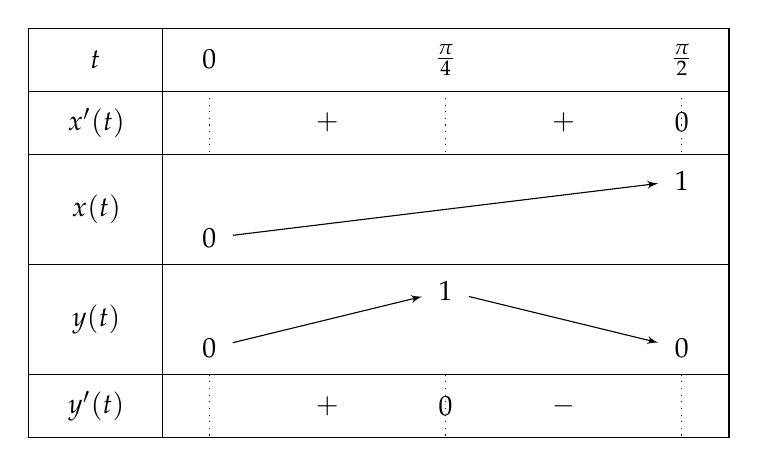
\begin{tikzpicture}
\tkzTabInit[lgt=1.7,espcl=3,deltacl=0.6]{$t$/0.8,$x'(t)$/0.8,$x(t)$/1.4,$y(t)$/1.4,$y'(t)$/0.8}{$0$,$\frac\pi4$,$\frac\pi2$}
\tkzTabLine{t,+,t,+,z}
\tkzTabVar{-/$0$,R/,+/$1$}
\tkzTabVar{-/$0$,+/$1$,-/$0$}
\tkzTabLine{t,+,z,-,t}
\end{tikzpicture}
\end{center}

\etape{Points remarquables} $O$ : $f'(0)=(1,2)$, tangente $y=2x$ ; $M\left(\frac\pi4\right)=\left(\frac{\sqrt2}2,1\right)$ : tangente
horizontale ; $M\left(\frac\pi2\right)=(1,0)$ : $f'=(0,-2)$, tangente verticale.

\etape{Point double} $O$ est atteint pour $t=0$ et $t=\pi$, avec $f'(\pi)=(-1,2)$ : tangentes $y=2x$ et $y=-2x$.

\etape{Tracé et cohérence} L'arc d'étude va de $O$ à $(1,0)$ en passant par le sommet $\left(\frac{\sqrt2}2,1\right)$ ; la symétrie
d'axe $(Ox)$ donne la boucle de droite, la symétrie de centre $O$ celle de gauche. La courbe a la forme d'un huit, et les
deux tangentes en $O$ se croisent bien comme sur la figure.

\begin{figure}[H]
\centering
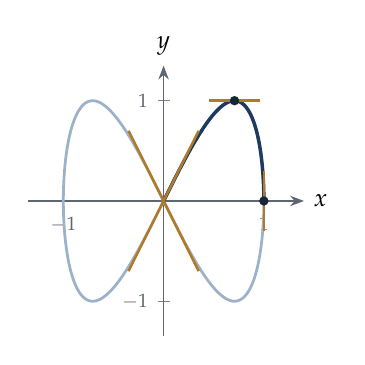
\begin{tikzpicture}
\begin{axis}[courbe,width=0.48\linewidth,xmin=-1.35,xmax=1.4,ymin=-1.35,ymax=1.35,xtick={-1,1},ytick={-1,1}]
\addplot[reste,domain=0:2*pi,samples=300]({sin(x)},{sin(2*x)});
\addplot[arcetude,domain=0:pi/2,samples=150]({sin(x)},{sin(2*x)});
\draw[tgte] (axis cs:-0.35,-0.7)--(axis cs:0.35,0.7); \draw[tgte] (axis cs:-0.35,0.7)--(axis cs:0.35,-0.7);
\draw[tgte] (axis cs:0.45,1)--(axis cs:0.96,1); \draw[tgte] (axis cs:1,-0.3)--(axis cs:1,0.3);
\node[pt] at (axis cs:0.7071,1) {}; \node[pt] at (axis cs:1,0) {};
\end{axis}
\end{tikzpicture}
\caption{La courbe $(\sin t,\sin2t)$ et ses tangentes remarquables.}
\end{figure}

% ...........................................................
\subsubsection{Une courbe à points singuliers : la cycloïde}

\begin{exemple}\label{ex:cycloide}
Une roue de rayon $1$ roule sans glisser sur $(Ox)$. Lorsqu'elle a tourné d'un angle $t$, le point de contact a parcouru
la longueur d'arc $t$ : le centre est en $C(t,1)$, et un point $M$ de la circonférence, initialement en $O$, vérifie
$\vv{CM}=(-\sin t,-\cos t)$. Étudier la courbe $M(t)=(t-\sin t,\ 1-\cos t)$.
\end{exemple}

\etape{Réduction} $f(t+2\pi)=f(t)+(2\pi,0)$ : invariance par translation, étude sur $[-\pi,\pi]$ ; $x$ impaire, $y$ paire :
symétrie d'axe $(Oy)$, étude sur $[0,\pi]$.

\etape{Variations} $x'=1-\cos t\geq0$, $y'=\sin t\geq0$ sur $[0,\pi]$ : $x$ croît de $0$ à $\pi$, $y$ de $0$ à $2$. En $\pi$,
$f'(\pi)=(2,0)$ : tangente horizontale au sommet $(\pi,2)$.

\etape{Points singuliers} $f'(t)=\ve0\iff t\in2\pi\Z$. En $0$ : $x=\frac{h^3}6+o(h^3)$, $y=\frac{h^2}2+o(h^3)$, donc
$f(h)=h^2\left(0,\frac12\right)+h^3\left(\frac16,0\right)+o(h^3)$ : $p=2$, $q=3$, rebroussement de première espèce à tangente
\emph{verticale}. Par translation, il en est de même en chaque $(2k\pi,0)$ : la courbe a une infinité de points singuliers,
qui correspondent aux instants où le point touche le sol.

\etape{Cohérence} Au point de contact, la vitesse du point de la roue est nulle : c'est la définition du roulement sans
glissement, et c'est ce que traduit $f'(2k\pi)=\ve0$.

\begin{figure}[H]
\centering
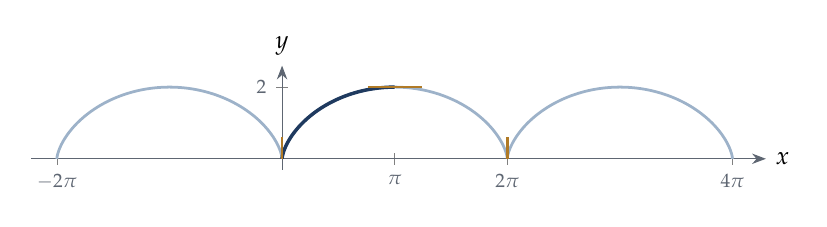
\begin{tikzpicture}
\begin{axis}[courbe,width=0.9\linewidth,xmin=-7,xmax=13.5,ymin=-0.3,ymax=2.6,
  xtick={-6.283,3.1416,6.283,12.566},xticklabels={$-2\pi$,$\pi$,$2\pi$,$4\pi$},ytick={2}]
\addplot[reste,domain=-2*pi:4*pi,samples=500]({x-sin(x)},{1-cos(x)});
\addplot[arcetude,domain=0:pi,samples=150]({x-sin(x)},{1-cos(x)});
\draw[tgte](axis cs:2.4,2)--(axis cs:3.9,2);
\draw[tgte](axis cs:0,0)--(axis cs:0,0.6);\draw[tgte](axis cs:6.283,0)--(axis cs:6.283,0.6);
\end{axis}
\end{tikzpicture}
\caption{La cycloïde : rebroussements à tangente verticale aux points $(2k\pi,0)$.}
\end{figure}

% ...........................................................
\subsubsection{Deux asymptotes}

\begin{exemple}\label{ex:g4}
Étudier et tracer $f(t)=\left(\dfrac t{t-1},\dfrac{t^2}{t-1}\right)$, $t\neq1$.
\end{exemple}

\etape{Premières observations} Pas de symétrie évidente. Une valeur interdite, $t=1$, et deux bornes $\pm\infty$ : trois
branches infinies possibles.

\etape{Dérivées} $x'(t)=-\dfrac1{(t-1)^2}<0$ : courbe régulière, $x$ toujours décroissante. $y'(t)=\dfrac{t(t-2)}{(t-1)^2}$ :
tangentes horizontales en $t=0$ (point $O$) et $t=2$ (point $(2,4)$).

\etape{Tableau}
\begin{center}
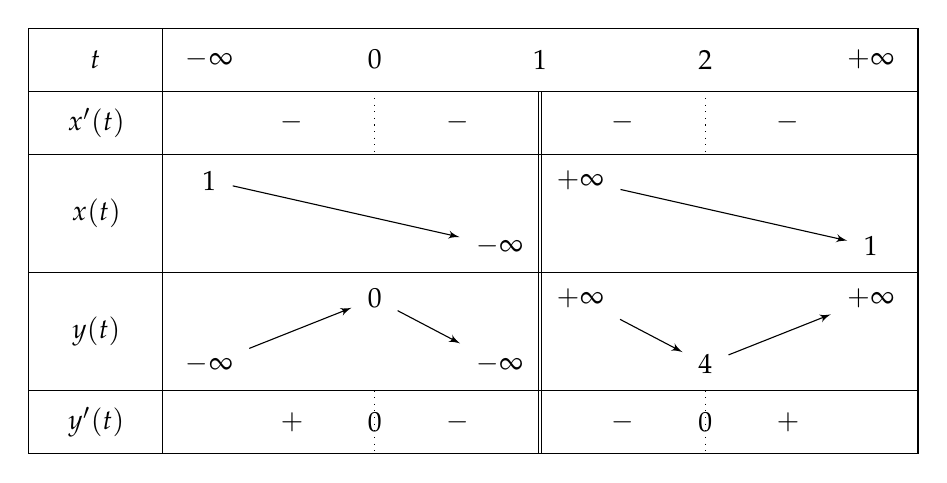
\begin{tikzpicture}
\tkzTabInit[lgt=1.7,espcl=2.1,deltacl=0.6]{$t$/0.8,$x'(t)$/0.8,$x(t)$/1.5,$y(t)$/1.5,$y'(t)$/0.8}{$-\infty$,$0$,$1$,$2$,$+\infty$}
\tkzTabLine{,-,t,-,d,-,t,-,}
\tkzTabVar{+/$1$,R/,-D+/$-\infty$/$+\infty$,R/,-/$1$}
\tkzTabVar{-/$-\infty$,+/$0$,-D+/$-\infty$/$+\infty$,-/$4$,+/$+\infty$}
\tkzTabLine{,+,z,-,d,-,z,+,}
\end{tikzpicture}
\end{center}
(On a $x(0)=0$ et $x(2)=2$.)

\etape{Branches infinies}
\begin{itemize}
\item $t\to\pm\infty$ : $x=1+\frac1{t-1}\to1$ et $y\sim t\to\pm\infty$ : asymptote verticale $x=1$ ; la courbe est à gauche
      ($x<1$) en bas lorsque $t\to-\infty$, à droite en haut lorsque $t\to+\infty$.
\item $t\to1$ : asymptote oblique $y=x+1$, avec $y-x-1=t-1$ : au-dessous côté $x\to-\infty$, au-dessus côté $x\to+\infty$.
\end{itemize}

\etape{Cohérence} En éliminant $t=\frac{x}{x-1}$, on trouve $y=\frac{x^2}{x-1}$ : le support est le graphe d'une fonction
rationnelle, ce qui confirme les deux asymptotes et les deux extremums $(0,0)$ et $(2,4)$.

\begin{figure}[H]
\centering
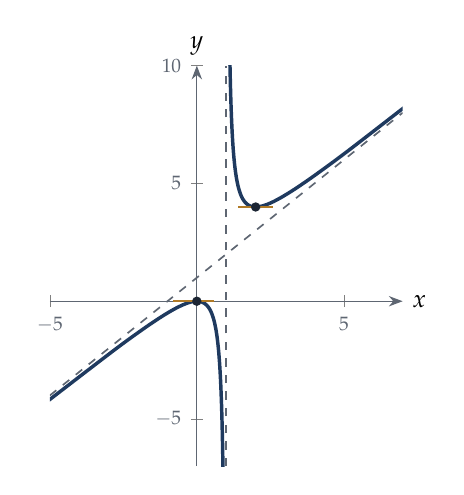
\begin{tikzpicture}
\begin{axis}[courbe,width=0.5\linewidth,xmin=-5,xmax=7,ymin=-7,ymax=10,axis equal image=false,height=0.55\linewidth,
  unbounded coords=jump,restrict y to domain=-20:20]
\addplot[asy,samples=2] coordinates {(1,-7) (1,10)};
\addplot[asy,domain=-5:7,samples=2]{x+1};
\addplot[arcetude,domain=-30:0.84,samples=300]({x/(x-1)},{x^2/(x-1)});
\addplot[arcetude,domain=1.14:30,samples=300]({x/(x-1)},{x^2/(x-1)});
\draw[tgte] (axis cs:-0.8,0)--(axis cs:0.6,0); \draw[tgte] (axis cs:1.4,4)--(axis cs:2.6,4);
\node[pt] at (axis cs:0,0) {}; \node[pt] at (axis cs:2,4) {};
\end{axis}
\end{tikzpicture}
\caption{La courbe $\left(\frac t{t-1},\frac{t^2}{t-1}\right)$ et ses asymptotes $x=1$ et $y=x+1$.}
\end{figure}

% ...........................................................
\subsubsection{Développement limité, inflexion et asymptote}

\begin{exemple}\label{ex:g5}
Étudier et tracer $f(t)=\left(\dfrac{t^3}{1+t^2},\dfrac{t}{1+t^4}\right)$.
\end{exemple}

\etape{Réduction} $x$ et $y$ impaires : symétrie de centre $O$, étude sur $[0,+\infty[$.

\etape{Dérivées} $x'(t)=\dfrac{t^2(t^2+3)}{(1+t^2)^2}\geq0$, $y'(t)=\dfrac{1-3t^4}{(1+t^4)^2}$. En $0$, $f'(0)=(0,1)$ : point régulier à
tangente verticale. En $t_1=3^{-1/4}\approx0{,}76$ : tangente horizontale, en $\left(x(t_1),\frac{3^{3/4}}4\right)\approx(0{,}28\,;\,0{,}57)$.

\etape{Tableau}
\begin{center}
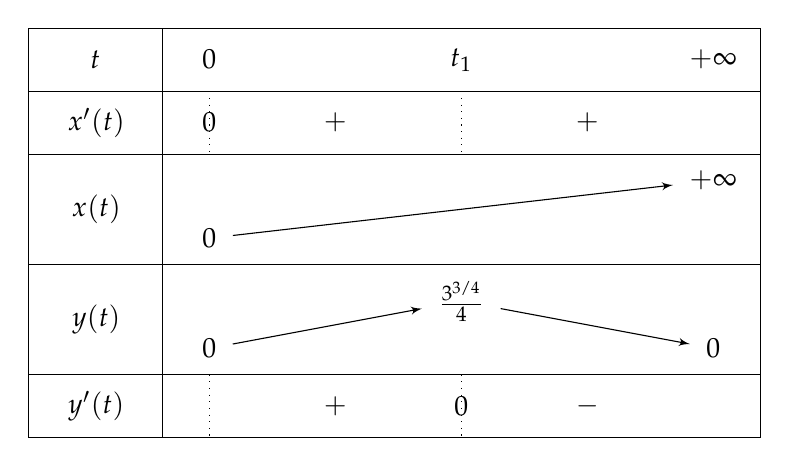
\begin{tikzpicture}
\tkzTabInit[lgt=1.7,espcl=3.2,deltacl=0.6]{$t$/0.8,$x'(t)$/0.8,$x(t)$/1.4,$y(t)$/1.4,$y'(t)$/0.8}{$0$,$t_1$,$+\infty$}
\tkzTabLine{z,+,t,+,}
\tkzTabVar{-/$0$,R/,+/$+\infty$}
\tkzTabVar{-/$0$,+/$\frac{3^{3/4}}4$,-/$0$}
\tkzTabLine{t,+,z,-,}
\end{tikzpicture}
\end{center}

\etape{Branche infinie} $t\to+\infty$ : $x\sim t\to+\infty$, $y\sim t^{-3}\to0^+$ : asymptote horizontale $y=0$, courbe
au-dessus.

\etape{Nature du point $O$} Le point est régulier, mais la symétrie centrale invite à vérifier s'il est d'inflexion :
$f(t)=t\,(0,1)+t^3(1,0)+o(t^3)$, donc $p=1$, $q=3$ : inflexion. C'est géométriquement inévitable : deux arcs symétriques par
rapport à un point de la courbe sont de part et d'autre de la tangente.

\begin{figure}[H]
\centering
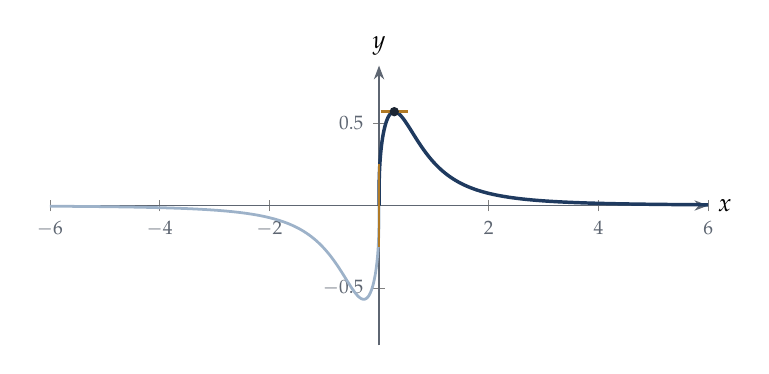
\begin{tikzpicture}
\begin{axis}[courbe,width=0.82\linewidth,xmin=-6,xmax=6,ymin=-0.85,ymax=0.85,unit vector ratio*=1 3,ytick={-0.5,0.5}]
\addplot[reste,domain=-6.2:0,samples=300]({x^3/(1+x^2)},{x/(1+x^4)});
\addplot[arcetude,domain=0:6.2,samples=300]({x^3/(1+x^2)},{x/(1+x^4)});
\draw[tgte] (axis cs:0.03,0.570)--(axis cs:0.53,0.570);
\draw[tgte] (axis cs:0,-0.25)--(axis cs:0,0.25);
\node[pt] at (axis cs:0.278,0.570) {};
\end{axis}
\end{tikzpicture}
\caption{Inflexion en $O$, asymptote $y=0$ (échelle verticale dilatée d'un facteur 3).}
\end{figure}

% ...........................................................
\subsubsection{Plusieurs difficultés : la cardioïde}

\begin{exemple}\label{ex:g6}
Étudier et tracer $f(t)=(2\cos t-\cos2t,\ 2\sin t-\sin2t)$.
\end{exemple}

\etape{Réduction} $2\pi$-périodique ; $x$ paire, $y$ impaire : symétrie d'axe $(Ox)$, étude sur $[0,\pi]$.

\etape{Dérivées factorisées} $x'(t)=2\sin t\,(2\cos t-1)$ et, par $\cos p-\cos q=-2\sin\frac{p+q}2\sin\frac{p-q}2$,
$y'(t)=2(\cos t-\cos2t)=4\sin\frac{3t}2\sin\frac t2$. Sur $[0,\pi]$ : $x'=0$ en $0,\frac\pi3,\pi$ ; $y'=0$ en $0,\frac{2\pi}3$. Seul
$t=0$ est singulier.

\etape{Tableau}
\begin{center}
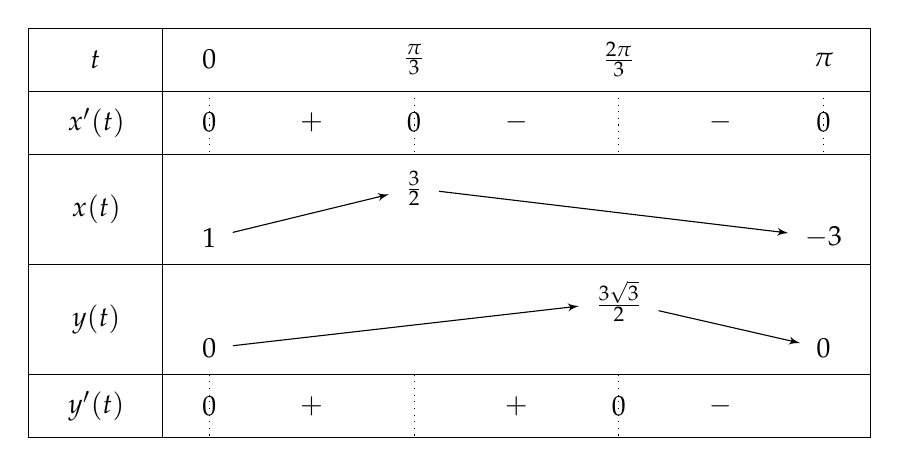
\begin{tikzpicture}
\tkzTabInit[lgt=1.7,espcl=2.6,deltacl=0.6]{$t$/0.8,$x'(t)$/0.8,$x(t)$/1.4,$y(t)$/1.4,$y'(t)$/0.8}{$0$,$\frac\pi3$,$\frac{2\pi}3$,$\pi$}
\tkzTabLine{z,+,z,-,t,-,z}
\tkzTabVar{-/$1$,+/$\frac32$,R/,-/$-3$}
\tkzTabVar{-/$0$,R/,+/$\frac{3\sqrt3}2$,-/$0$}
\tkzTabLine{z,+,t,+,z,-,}
\end{tikzpicture}
\end{center}

\etape{Point singulier} En $0$ : $x(h)=1+h^2-\frac7{12}h^4+o(h^4)$ et $y(h)=h^3+o(h^3)$, donc
$f(h)=(1,0)+h^2(1,0)+h^3(0,1)+o(h^3)$ : rebroussement de première espèce, tangente horizontale.

\etape{Tracé et cohérence} Tangente verticale en $\left(\frac32,\frac{\sqrt3}2\right)$ et $(-3,0)$, horizontale en
$\left(-\frac12,\frac{3\sqrt3}2\right)$. Le rebroussement en $(1,0)$ pointe vers l'intérieur de la courbe : la courbe y arrive en
allant vers la droite ($\ve a=(1,0)$, $h^2>0$), ce que confirme $x'>0$ sur $]0,\frac\pi3[$.

\begin{figure}[H]
\centering
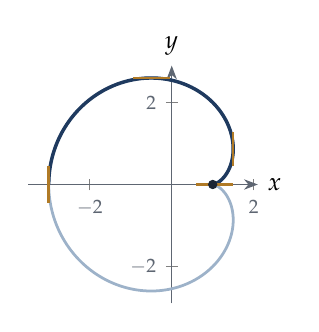
\begin{tikzpicture}
\begin{axis}[courbe,width=0.44\linewidth,xmin=-3.5,xmax=2.1,ymin=-2.9,ymax=2.9]
\addplot[reste,domain=0:2*pi,samples=400]({2*cos(x)-cos(2*x)},{2*sin(x)-sin(2*x)});
\addplot[arcetude,domain=0:pi,samples=200]({2*cos(x)-cos(2*x)},{2*sin(x)-sin(2*x)});
\draw[tgte](axis cs:1.5,0.45)--(axis cs:1.5,1.28);
\draw[tgte](axis cs:-0.95,2.598)--(axis cs:-0.05,2.598);
\draw[tgte](axis cs:-3,-0.45)--(axis cs:-3,0.45);
\draw[tgte](axis cs:0.6,0)--(axis cs:1.5,0);
\node[pt] at (axis cs:1,0) {};
\end{axis}
\end{tikzpicture}
\caption{La cardioïde.}
\end{figure}

% ---------------------------------------------------------------------
\subsubsection{Une courbe de Lissajous : point double, intersection, inflexions}

Cet exemple reprend, sur une autre courbe, les trois questions traitées en cours sur la courbe de Lissajous
$(\cos3t,2\sin t)$ : tangentes en un point double, intersection d'une tangente avec la courbe, recherche des points
d'inflexion.

\begin{exemple}\label{ex:g7}
Étudier la courbe $f(t)=(\cos t,\ \sin3t)$ ; déterminer ses points doubles et les tangentes en ces points, les autres
points d'intersection de la courbe avec l'une de ces tangentes, puis ses points d'inflexion.
\end{exemple}

\etape{Réduction} $f$ est $2\pi$-périodique. $f(-t)=(x(t),-y(t))$ : symétrie d'axe $(Ox)$. $f(\pi-t)=(-\cos t,\sin(3\pi-3t))=
(-x(t),y(t))$ : symétrie d'axe $(Oy)$. On étudie sur $\left[0,\frac\pi2\right]$, puis on complète par la symétrie d'axe
$(Oy)$ (on obtient $[0,\pi]$), enfin par celle d'axe $(Ox)$.

\etape{Variations} $x'(t)=-\sin t$ et $y'(t)=3\cos3t$ ne s'annulent jamais ensemble : la courbe est régulière.
\begin{center}
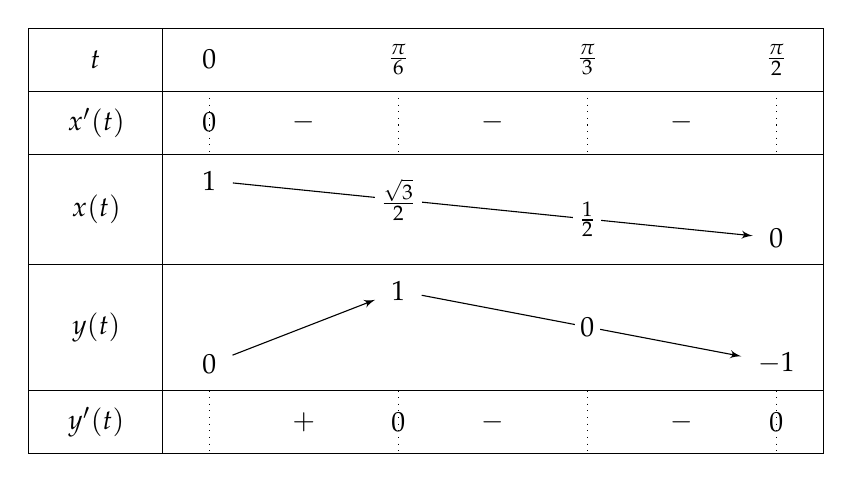
\begin{tikzpicture}
\tkzTabInit[lgt=1.7,espcl=2.4,deltacl=0.6]{$t$/0.8,$x'(t)$/0.8,$x(t)$/1.4,$y(t)$/1.6,$y'(t)$/0.8}{$0$,$\frac\pi6$,$\frac\pi3$,$\frac\pi2$}
\tkzTabLine{z,-,t,-,t,-,t}
\tkzTabVar{+/$1$,R/,R/,-/$0$}
\tkzTabIma{1}{4}{2}{$\frac{\sqrt3}2$}
\tkzTabIma{1}{4}{3}{$\frac12$}
\tkzTabVar{-/$0$,+/$1$,R/,-/$-1$}
\tkzTabIma{2}{4}{3}{$0$}
\tkzTabLine{t,+,z,-,t,-,z}
\end{tikzpicture}
\end{center}
Tangente verticale en $M(0)=(1,0)$ (point de l'axe $(Ox)$, tangente perpendiculaire à l'axe) ; tangentes horizontales en
$M\left(\frac\pi6\right)=\left(\frac{\sqrt3}2,1\right)$ et en $M\left(\frac\pi2\right)=(0,-1)$, point de l'axe $(Oy)$.

\etape{Point double} Sur $[0,\pi]$, la courbe coupe l'axe $(Ox)$ lorsque $\sin3t=0$, soit en $t=0,\frac\pi3,\frac{2\pi}3,\pi$.
En $M\left(\frac\pi3\right)=\left(\frac12,0\right)$, la tangente n'est pas perpendiculaire à l'axe : la courbe le traverse
en biais, et la symétrie d'axe $(Ox)$ fournit un second arc, parcouru pour $t$ voisin de $-\frac\pi3$, qui passe par le même
point. La courbe passe donc deux fois par
$\left(\frac12,0\right)$ (et, par symétrie, par $\left(-\frac12,0\right)$). Comme $f'\left(\frac\pi3\right)=\left(-\frac{\sqrt3}2,-3\right)$ et
$f'\left(-\frac\pi3\right)=\left(\frac{\sqrt3}2,-3\right)$, les deux tangentes ont pour pentes $2\sqrt3$ et $-2\sqrt3$ :
\[T_1:y=2\sqrt3\left(x-\tfrac12\right),\qquad T_2:y=-2\sqrt3\left(x-\tfrac12\right).\]

\etape{Intersection de $T_1$ et de la courbe} $M(t)\in T_1\iff\sin3t=\sqrt3(2\cos t-1)$. On écrit tout en fonction de
$X=\cos t$, avec $\sin3t=3\sin t-4\sin^3t=\sin t\,(4\cos^2t-1)$ :
\[\sin t\,(4X^2-1)=\sqrt3\,(2X-1).\]
En élevant au carré (ce qui impose une vérification finale des signes) et en remplaçant $\sin^2t$ par $1-X^2$ :
\[(1-X^2)(2X-1)^2(2X+1)^2=3(2X-1)^2\iff(2X-1)^3\,(2X^3+3X^2-2)=0,\]
car $(1-X^2)(2X+1)^2-3=-(2X-1)(2X^3+3X^2-2)$. La racine \emph{triple} $X=\frac12$ s'interprète : la tangence en
$t=\frac\pi3$ compte deux fois, le passage de l'autre branche ($t=-\frac\pi3$) une fois. Le polynôme $2X^3+3X^2-2$ a une
seule racine réelle (ses extremums locaux, en $-1$ et $0$, valent $-1$ et $-2$), $X_0\approx0{,}678$. L'équation non
élevée au carré impose $\sin t>0$ (les deux autres facteurs sont positifs) : $t_0=\arccos X_0\approx0{,}826$, et $T_1$
recoupe la courbe en un seul autre point, $P\approx(0{,}678\,;0{,}615)$.

\etape{Inflexions} $f''(t)=(-\cos t,-9\sin3t)$ et, en linéarisant,
\[\det\big(f'(t),f''(t)\big)=9\sin t\sin3t+3\cos t\cos3t=6\cos2t-3\cos4t=-3\,(2c^2-2c-1),\]
où $c=\cos2t$ (on a utilisé $\cos4t=2c^2-1$).
Le déterminant s'annule pour $c=\frac{1-\sqrt3}2$ (l'autre racine est supérieure à $1$). Sur $\left[0,\frac\pi2\right]$,
$c=\cos2t$ décroît strictement : il existe un unique $\alpha=\frac12\arccos\frac{1-\sqrt3}2\approx0{,}973$, et le
déterminant change de signe en $\alpha$ (racine simple). Le point $M(\alpha)\approx(0{,}563\,;0{,}221)$ est un point
d'inflexion ; par symétrie, la courbe en a quatre. Le cours obtient la même équation sous la forme
$\tan t\tan3t=-\frac13$ en posant $u=\tan t$ ; la linéarisation est ici plus courte.

\begin{figure}[H]
\centering
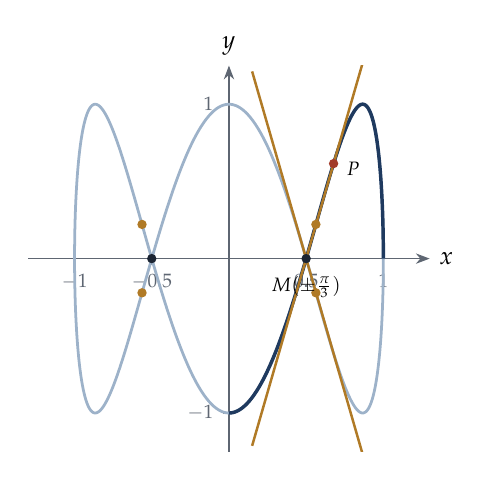
\begin{tikzpicture}
\begin{axis}[courbe,width=0.62\linewidth,xmin=-1.3,xmax=1.3,ymin=-1.25,ymax=1.25,xtick={-1,-0.5,0.5,1},ytick={-1,1}]
\addplot[reste,domain=0:6.2832,samples=400]({cos(x)},{sin(3*x)});
\addplot[arcetude,domain=0:1.5708,samples=200]({cos(x)},{sin(3*x)});
\addplot[tgte,domain=0.15:0.95,samples=2]{2*sqrt(3)*(x-0.5)};
\addplot[tgte,domain=0.15:0.95,samples=2]{-2*sqrt(3)*(x-0.5)};
\node[pt] at (axis cs:0.5,0) {}; \node[pt] at (axis cs:-0.5,0) {};
\node[pt,fill=Brique] at (axis cs:0.6777,0.6154) {}; \node[font=\scriptsize,anchor=west] at (axis cs:0.70,0.58) {$P$};
\node[pt,fill=Ocre] at (axis cs:0.5630,0.2214) {}; \node[pt,fill=Ocre] at (axis cs:-0.5630,0.2214) {};
\node[pt,fill=Ocre] at (axis cs:0.5630,-0.2214) {}; \node[pt,fill=Ocre] at (axis cs:-0.5630,-0.2214) {};
\node[font=\scriptsize,anchor=north] at (axis cs:0.5,-0.05) {$M(\pm\frac\pi3)$};
\end{axis}
\end{tikzpicture}
\caption{La courbe $(\cos t,\sin3t)$ ; en trait plein l'arc d'étude $\left[0,\frac\pi2\right]$, en ocre les tangentes au
point double $\left(\frac12,0\right)$ et les quatre points d'inflexion, en brique le point $P$ où $T_1$ recoupe la courbe.}
\end{figure}

\subsection{Paramétrer et reconnaître une courbe}

Lorsqu'un paramétrage rappelle une identité connue, on élimine $t$ : $(2\cos t,3\sin t)$ vérifie
$\frac{x^2}4+\frac{y^2}9=1$ (ellipse), $(t^2,2t)$ vérifie $y^2=4x$ (parabole), $(\ch t,\sh t)$ vérifie $x^2-y^2=1$. On
obtient une \emph{inclusion} du support dans la courbe d'équation ; l'égalité se vérifie à part. Inversement, pour
paramétrer une courbe donnée par une équation, on cherche un paramètre naturel : un angle, une coordonnée, ou la pente
$t=y/x$ de la droite $(OM)$.

\begin{exemple}[paramétrer un cercle par la pente]\label{ex:cercle-pente}
Soit $\mathcal C:x^2+y^2=2x$. Pour $M\neq O$ sur $\mathcal C$, on pose $t=\frac yx$. En remplaçant $y$ par $tx$ :
$x^2(1+t^2)=2x$, d'où $x=\frac2{1+t^2}$ et $y=\frac{2t}{1+t^2}$ : $M(t)$ est le second point d'intersection du cercle avec
la droite $y=tx$.
\end{exemple}

% ---------------------------------------------------------------------
\subsection{Fiches pratiques}

\begin{tcolorbox}[enhanced,breakable,colback=Fond,colframe=Fond,arc=0pt,boxrule=0pt,left=12pt,right=12pt,top=10pt,bottom=10pt,
  borderline north={1.4pt}{0pt}{Bleu}]
\phantomsection\label{fiche:1}{\sffamily\bfseries\color{Bleu}FICHE 1 --- Tracer une courbe paramétrée sans oublier aucune étape}\par\medskip
\begin{enumerate}
\item Ensemble de définition ; \textbf{noter les valeurs interdites}.
\item Parités, périodicité, $f(\pi-t)$, $f(1/t)$ ; intervalle d'étude ; \textbf{noter l'ordre des réductions}.
\item Limites de $x$ et $y$ à toutes les bornes, des deux côtés des valeurs interdites.
\item $x'$ et $y'$ \textbf{factorisées} ; zéros communs = points singuliers.
\item Tableau conjoint $t$, $x'$, $x$, $y$, $y'$.
\item Tangentes : horizontales ($y'=0\neq x'$), verticales ($x'=0\neq y'$) ; points singuliers par développement limité.
\item Branches infinies : limites de $x$, $y$, puis $y/x$, puis $y-ax$ ; positions.
\item Points doubles, intersections avec les axes si utile.
\item Tracé : axes, asymptotes, points et tangentes, arcs selon le tableau, symétries, flèches de parcours.
\item Vérification sur un point calculé et sur chaque ligne du tableau.
\end{enumerate}
\end{tcolorbox}

\begin{tcolorbox}[enhanced,breakable,colback=white,colframe=white,arc=0pt,boxrule=0pt,left=4pt,right=4pt,top=10pt,bottom=6pt,
  borderline north={1.4pt}{0pt}{Brique}]
\phantomsection\label{fiche:2}{\sffamily\bfseries\color{Brique}FICHE 2 --- Les erreurs classiques et comment les corriger}\par\medskip
\small
\renewcommand{\arraystretch}{1.3}
\begin{tabular}{>{\raggedright}p{0.3\linewidth}>{\raggedright}p{0.3\linewidth}p{0.3\linewidth}}
\toprule
\sffamily Erreur & \sffamily Comment la détecter & \sffamily Comment la corriger\\\midrule
Croire qu'un vecteur vitesse nul empêche toute tangente & on a écrit « pas de tangente » en un point où $f'=\ve0$ & développement limité : la tangente est dirigée par $f^{(p)}(t_0)$\tabularnewline
Oublier le sens de parcours & les arcs sont reliés dans un ordre qui contredit le tableau & dessiner des flèches selon le signe de $(x',y')$\tabularnewline
Déduire une asymptote d'une direction asymptotique & on a seulement calculé $\lim y/x$ & calculer $\lim(y-ax)$ avant de conclure\tabularnewline
Négliger la position relative & la courbe coupe son asymptote près de l'infini sur le dessin & étudier le signe de $y-ax-b$ de chaque côté\tabularnewline
Oublier les symétries & la figure n'a pas la symétrie prévue, ou l'on a fait deux fois les calculs & tester $f(-t)$, $f(t+T)$ dès le début\tabularnewline
Tracer une branche sans tenir compte des limites & une extrémité d'arc ne correspond à aucune limite du tableau & reporter toutes les limites aux bornes avant de tracer\tabularnewline
Relier les points sans respecter les variations & un arc monte alors que $y$ décroît sur l'intervalle & suivre les signes de $x'$ et $y'$ intervalle par intervalle\tabularnewline
Confondre allure locale et allure globale & une pointe dessinée à un point régulier, ou un arc lisse à un point singulier & n'utiliser le développement limité qu'au voisinage du point étudié\tabularnewline
\bottomrule
\end{tabular}
\end{tcolorbox}

% ---------------------------------------------------------------------
\subsection{Exercices de tracé}

Les séries suivent la progression du chapitre : on ne passe à la suivante qu'après avoir réussi la précédente.

\serie{Série 1 --- Tangentes et points singuliers}

\rappel{développements limités en $0$} $\frac1{1+u}=1-u+u^2-u^3+o(u^3)$, $\ln(1+u)=u-\frac{u^2}2+\frac{u^3}3+o(u^3)$,
$e^u=1+u+\frac{u^2}2+\frac{u^3}6+o(u^3)$, $\cos u=1-\frac{u^2}2+o(u^3)$, $\sin u=u-\frac{u^3}6+o(u^3)$.

\begin{exo}{loc-b}{2}{développement limité en un point stationnaire}
Vérifier que $M(0)$ est stationnaire pour $f(t)=(e^t-t,\ t^3)$, et déterminer sa nature et sa tangente.
\end{exo}
\begin{exo}{loc-c}{3}{changement de variable $t=t_0+h$}
On reprend $f(t)=\left(t+\frac1t,\ t\ln t-t\right)$, dont le point $M(1)$ est stationnaire (exercice~\ref{e:tg-c}).
Déterminer la nature de ce point et la direction de la tangente.
\end{exo}
\begin{exo}{loc-d}{3}{colinéarité de $f'$ et $f''$ ; inflexions}
Soit $f(t)=(\cos t,\sin^3t)$, $t\in[-\pi,\pi]$. Déterminer les valeurs de $t_0$ pour lesquelles $f'(t_0)$ et $f''(t_0)$
sont colinéaires ; préciser lesquelles correspondent à des points réguliers, et conclure.
\end{exo}

\serie{Série 2 --- Branches infinies}

\rappel{croissances comparées} Pour $\alpha,\beta>0$ : $\frac{t^\alpha}{e^{\beta t}}\to0$ et $\frac{(\ln t)^\beta}{t^\alpha}\to0$ quand
$t\to+\infty$. Les développements limités de la série 1 servent aussi aux développements asymptotiques.

\begin{exo}{br-b}{3}{inflexion ; branches paraboliques}
Étudier les points d'inflexion et les branches infinies de la courbe $f(t)=(e^t,t^2)$, $t\in\R$.
\end{exo}
\begin{exo}{br-c}{4}{asymptote oblique ; position ; point limite et prolongement}
Soit $\mathcal C$ la courbe $f(t)=\left(\dfrac1t,\dfrac1{e^t-1}\right)$, $t\in\R^*$.
\begin{enumerate}
\item Déterminer l'asymptote $\mathcal A$ lorsque $t\to0$ et la position de la courbe par rapport à $\mathcal A$.
\item Montrer que, lorsque $t\to+\infty$, $M(t)$ tend vers un point $A$ ; déterminer la tangente à la courbe prolongée en $A$.
\item Même question lorsque $t\to-\infty$.
\item En déduire le tracé de $\mathcal C$.
\end{enumerate}
\end{exo}

\serie{Série 3 --- Tracés partiels et reconnaissance}

\rappel{fonctions hyperboliques} $\ch t=\frac{e^t+e^{-t}}2$, $\sh t=\frac{e^t-e^{-t}}2$, $\th t=\frac{\sh t}{\ch t}$,
$\ch^2t-\sh^2t=1$, $\ch'=\sh$, $\sh'=\ch$, $\th'=1-\th^2$ ; $\ch$ est paire, $\sh$ et $\th$ impaires ;
$\sh t=a\iff t=\argsh a=\ln\big(a+\sqrt{a^2+1}\big)$ ; $\th t=t-\frac{t^3}3+o(t^3)$.

\begin{exo}{rec-hyp}{2}{élimination du paramètre ; égalité d'ensembles}
Soit $\Gamma$ la courbe $t\mapsto(\ch t,\sh t)$, $t\in\R$.
\begin{enumerate}
\item Étudier et tracer $\Gamma$.
\item Donner une équation vérifiée par chaque point du support.
\item L'ensemble défini par cette équation est-il égal au support de $\Gamma$ ?
\end{enumerate}
\end{exo}
\begin{exo}{rec-astro}{2}{élimination du paramètre}
Montrer que le support de $f(t)=(\cos^3t,\sin^3t)$ est inclus dans la courbe d'équation $x^{2/3}+y^{2/3}=1$, en
interprétant $x^{2/3}$ comme $(x^{1/3})^2$ pour $x$ réel.
\end{exo}
\begin{exo}{rec-x4}{3}{paramétrage par un angle}
Paramétrer et tracer la courbe $\mathcal C$ d'équation $x^4+y^2=1$. On exploitera les symétries de l'équation et l'on
posera $x^2=\cos\theta$.
\end{exo}

\serie{Série 4 --- Tracés complets}

\begin{exo}{b-noeud}{3}{étude complète, point double}
Étudier et tracer la courbe $f(t)=(t^2,\ t^3-t)$, $t\in\R$. On montrera que la courbe passe deux fois par le point
$(1,0)$ et l'on donnera les tangentes en ce point.
\end{exo}
\begin{exo}{b-astro}{4}{trois symétries, rebroussements, propriété d'une tangente}
On considère l'astroïde $f(t)=(\cos^3t,\sin^3t)$.
\begin{enumerate}
\item Réduire l'intervalle d'étude à $\left[0,\frac\pi4\right]$ en précisant les symétries utilisées.
\item Étudier la courbe et la tracer.
\item Pour $t\notin\frac\pi2\Z$, la tangente en $M(t)$ coupe les axes en $P$ et $Q$. Montrer que $PQ=1$.
\end{enumerate}
\end{exo}

\serie{Série 5 --- Problèmes de synthèse}

Les formules sur les fonctions hyperboliques utiles ici sont rappelées au début de la série 3.

\begin{exo}{c-der}{1}{dérivées usuelles}
Dériver $t\mapsto te^{-t}$, $t\mapsto\ln(1+t^2)$, $t\mapsto\dfrac1{\ch t}$ et $t\mapsto t-\th t$.
\end{exo}
\begin{exo}{c-sh}{2}{fonctions hyperboliques}
Soit $t_0$ le réel tel que $\sh t_0=1$. Calculer $\ch t_0$ et $\th t_0$, puis exprimer $t_0$ à l'aide d'un logarithme.
\end{exo}
\begin{exo}{b-tract}{5}{fonctions hyperboliques ; tangentes ; propriété géométrique}
On considère la courbe $(\Gamma)$ : $x(t)=t-\th t$, $y(t)=\dfrac1{\ch t}$, $t\in\R$.
\begin{enumerate}
\item Étudier $(\Gamma)$.
\item Déterminer le point $A$ de $(\Gamma)$ où la tangente a pour coefficient directeur $-1$, et une équation de cette
      tangente. On utilisera l'exercice~\ref{e:c-sh}.
\item Pour $t\neq0$, on note $T_t$ la tangente en $M(t)$. Montrer que $T_t$ coupe l'axe $(Ox)$ en un unique point
      $N$, et calculer la distance $MN$.
\end{enumerate}
\end{exo}
\begin{exo}{b-folium}{5}{folium de Descartes : courbe implicite, symétrie $t\mapsto1/t$}
\begin{enumerate}
\item Paramétrer l'ensemble $\mathcal C$ d'équation $x^3+y^3=3xy$ en posant $y=tx$, comme dans
      l'exemple~\ref{ex:cercle-pente}.
\item Interpréter géométriquement le paramètre $t$ et le point $M(t)$.
\item Montrer que $M(1/t)$ est le symétrique de $M(t)$ par rapport à la droite $y=x$, et en déduire un intervalle
      d'étude.
\item Étudier et tracer $\mathcal C$.
\end{enumerate}
\end{exo}

\begin{essentiel}\label{ess:5}
\begin{itemize}
\item Plan : définition, symétries, limites, dérivées factorisées, tableau conjoint, tangentes, branches infinies, tracé.
\item Point singulier : développement limité jusqu'au premier vecteur non colinéaire ; $p$ pair = rebroussement.
\item Position par rapport à la tangente : signe de $h^q$ ; par rapport à une asymptote : signe de $y-ax-b$.
\item Direction asymptotique ($y/x\to a$) $\neq$ asymptote ($y-ax\to b$ en plus).
\item Le tableau guide le tracé : signes de $(x',y')$ = direction de déplacement.
\end{itemize}
\end{essentiel}
% =====================================================================
%            CHAPITRE 6 — ENTRAÎNEMENT NIVEAU TD ET DS
% =====================================================================
\clearpage
\section{Entraînement niveau TD et DS}\label{sec:entrainement}

Les chapitres précédents installent les notions et les méthodes. Ce chapitre prépare aux exercices tels qu'ils sont posés
en classe : énoncés plus longs, questions enchaînées, méthode non indiquée, calculs qui demandent de l'initiative. Les
exercices reprennent les techniques des feuilles de TD et du devoir surveillé, avec une difficulté comparable ou un peu
supérieure, et leurs corrigés expliquent d'abord \emph{pourquoi} telle méthode a été choisie.

\ouverture{%
\begin{itemize}
\item Reconnaître, sans indication, la méthode adaptée à un déterminant.
\item Mener seul l'étude complète d'une courbe, y compris les questions « de devoir » : position globale, courbe
      asymptote, inflexions, tangente de pente donnée.
\item Rédiger un problème long en gérant son temps.
\end{itemize}}{%
\begin{itemize}
\item Chapitres 4 et 5, en particulier la boîte à outils (section~\ref{sec:outils-td}).
\end{itemize}}{Trois à quatre heures en autonomie, ou une séance de deux heures consacrée au problème final.}

\begin{commencer}
Les outils utilisés ici sont rassemblés en deux endroits : pour les déterminants, l'encadré d'ouverture et les méthodes du
chapitre 4 ; pour les courbes, la méthode commentée et la boîte à outils du chapitre 5 (méthodes~\ref{meth:inflexion} et
\ref{meth:posglob}, encadré sur les courbes asymptotes). Chaque corrigé renvoie à la méthode qu'il applique.
\end{commencer}

% ---------------------------------------------------------------------
\subsection{Ce que demandent les TD et le devoir}

\begin{center}
\renewcommand{\arraystretch}{1.3}\small
\begin{tabular}{>{\raggedright}p{0.4\linewidth}>{\raggedright\arraybackslash}p{0.52\linewidth}}
\toprule
\sffamily Question type & \sffamily Où s'entraîner\\\midrule
Déterminant d'ordre $n$ donné par une formule ou par sa forme & méthode~\ref{meth:diff}, exemples~\ref{ex:max} et~\ref{ex:X}, exercice~\ref{e:det-choix}\\
Récurrence, suites récurrentes linéaires & méthode~\ref{meth:rec}, exercices~\ref{e:r-321} à~\ref{e:r-cheb}\\
Déterminant avec paramètre, fonction affine & méthode~\ref{meth:affine}, exercice~\ref{e:det-pb}\\
Endomorphisme défini géométriquement & proposition~\ref{prop:proj-sym}, exercices~\ref{e:g-proj} et~\ref{e:g-simil}\\\midrule
Tracer à partir d'un tableau donné & exercice~\ref{e:td-tab}\\
Lieu géométrique, tangence & exercice~\ref{e:echelle}\\
Point stationnaire en $t_0\neq0$, nature, position locale & méthode~\ref{meth:dl}, exercices~\ref{e:loc-e}, \ref{e:bicorne2}, problème~\ref{e:ds-pb}\\
Position globale par rapport à une tangente & méthode~\ref{meth:posglob}, problème~\ref{e:ds-pb}\\
Points d'inflexion, tangente de pente donnée & méthode~\ref{meth:inflexion}, exercice~\ref{e:infl2}\\
Asymptotes, courbe asymptote \HP, point limite & méthode~\ref{meth:branches}, exercices~\ref{e:cub-asy}, \ref{e:br-c}\\
Symétries, point double, équation cartésienne ou polaire \HP & exercices~\ref{e:strophoide}, \ref{e:lemni}, \ref{e:cardio2}\\\bottomrule
\end{tabular}
\end{center}

% ---------------------------------------------------------------------
\subsection{Série A --- Déterminants : choisir et combiner}

Ces deux exercices ne disent pas quelle méthode employer. Avant de calculer, on écrit en une phrase la structure repérée
et la méthode qu'elle appelle ; c'est ce que l'on attend dans une copie.

\begin{exo}{det-choix}{3}{choisir la méthode}
Calculer les déterminants suivants. Pour chacun, on indiquera d'abord la méthode choisie et pourquoi.
\[D_1=\dt{1+a&1&1\\1&1+a&1\\1&1&1+a},\qquad D_2=\dt{1&1&1\\a&b&c\\a^3&b^3&c^3},\]
\[D_3=\det\big(\cos(i+j)\big)_{1\leq i,j\leq n}\ (n\geq2),\qquad D_4=\det\big(i^{\,j-1}\big)_{1\leq i,j\leq n}.\]
\end{exo}
\coupdepouce{quatre déterminants, quatre méthodes : somme constante, polynôme, colonnes liées, Vandermonde.}
\begin{exo}{det-pb}{4}{fonction affine, parité, matrice antisymétrique}
Pour $n\geq2$ et $x\in\R$, soit $M_n(x)$ la matrice d'ordre $n$ ayant des $x$ sur la diagonale, des $1$ au-dessus et des $-1$
au-dessous.
\begin{enumerate}
\item En ajoutant une constante $c$ à tous les coefficients, montrer que $\det M_n(x)=\dfrac{(x+1)^n+(x-1)^n}2$.
\item Pour quelles valeurs de $x$ la matrice $M_n(x)$ est-elle inversible ? On distinguera selon la parité de $n$.
\item Retrouver le résultat de l'exercice~\ref{e:g-antisym} pour $x=0$.
\item Montrer que, pour $n=3$, les vecteurs colonnes de $M_3(x)$ forment une base de $\R^3$ si et seulement si $x\neq0$, et
      vérifier la formule par la règle de Sarrus.
\end{enumerate}
\end{exo}

% ---------------------------------------------------------------------
\subsection{Série B --- Courbes : exercices de TD}

Les exercices sont rangés par difficulté croissante. Les trois premiers isolent une compétence ; les suivants sont des
études complètes, du type des courbes classiques du TD (cissoïde, lemniscate, bicorne, cardioïde).

\begin{exo}{td-tab}{2}{lire un tableau de variations ; symétries ; injectivité}
Une courbe $f(t)=\big(x(t),y(t)\big)$, $t\in[0,\pi]$, a le tableau de variations suivant.
\begin{center}
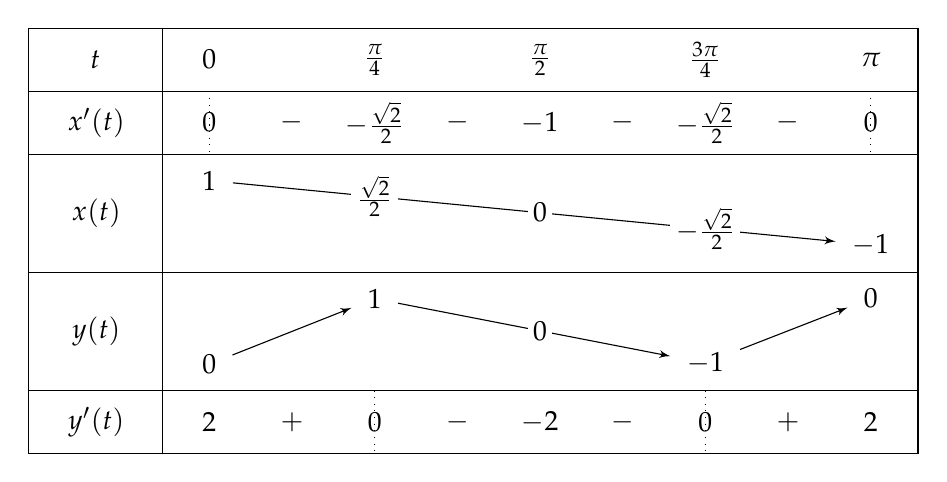
\begin{tikzpicture}
\tkzTabInit[lgt=1.7,espcl=2.1,deltacl=0.6]{$t$/0.8,$x'(t)$/0.8,$x(t)$/1.5,$y(t)$/1.5,$y'(t)$/0.8}{$0$,$\frac\pi4$,$\frac\pi2$,$\frac{3\pi}4$,$\pi$}
\tkzTabLine{z,-,-\frac{\sqrt2}2,-,-1,-,-\frac{\sqrt2}2,-,z}
\tkzTabVar{+/$1$,R/,R/,R/,-/$-1$}
\tkzTabIma{1}{5}{2}{$\frac{\sqrt2}2$}
\tkzTabIma{1}{5}{3}{$0$}
\tkzTabIma{1}{5}{4}{$-\frac{\sqrt2}2$}
\tkzTabVar{-/$0$,+/$1$,R/,-/$-1$,+/$0$}
\tkzTabIma{2}{4}{3}{$0$}
\tkzTabLine{2,+,z,-,-2,-,z,+,2}
\end{tikzpicture}
\end{center}
\begin{enumerate}
\item Placer les points remarquables avec leurs tangentes et dessiner l'arc $\Gamma_0=f([0,\pi])$.
\item Donner une équation de la tangente au point de paramètre $\frac\pi2$.
\item La restriction de $f$ à $[0,\pi]$ est-elle injective ? Que peut-on en déduire pour $\Gamma_0$ ?
\item On suppose maintenant $f$ définie sur $[-\pi,\pi]$.
\begin{enumerate}
\item Quelle est l'allure de la courbe si $x$ est paire et $y$ impaire ? Y a-t-il un point double ?
\item Et si $x$ et $y$ sont paires ?
\item La fonction $f$ peut-elle être impaire ? $\pi$-périodique ?
\end{enumerate}
\item Vérifier que $f(t)=(\cos t,\sin2t)$ a ce tableau.
\end{enumerate}
\end{exo}
\begin{exo}{echelle}{3}{lieu géométrique ; tangence ; enveloppe}
Une échelle $[PQ]$ de longueur $L=a+b$ ($a,b>0$) glisse : son pied $P$ reste sur le sol (l'axe $(Ox)$), son sommet $Q$
contre le mur (l'axe $(Oy)$). On note $\theta\in\left[0,\frac\pi2\right]$ l'angle entre l'échelle et le sol.
\begin{enumerate}
\item Exprimer $P$ et $Q$ en fonction de $\theta$. Soit $M$ le barreau tel que $QM=a$ et $MP=b$ : montrer que
      $M(\theta)=(a\cos\theta,\ b\sin\theta)$. Quelle est la trajectoire de $M$ ? Que se passe-t-il si $a=b$ ?
\item Pour $a=2$ et $b=1$, à quel moment l'échelle est-elle tangente à la trajectoire de $M$ ?
\item Soit $A(\theta)=(L\cos^3\theta,\ L\sin^3\theta)$. Montrer que $A(\theta)$ est sur l'échelle et que, pour
      $\theta\in\left]0,\frac\pi2\right[$, l'échelle est tangente en $A(\theta)$ à la courbe décrite par $A$.
\end{enumerate}
\end{exo}
\coupdepouce{« tangente » se traduit par « vecteur dérivé et direction de l'échelle colinéaires ».}
\begin{exo}{loc-e}{3}{développement limité avec racine et logarithme}
Soit $f(t)=\big(t-\ln(1+t),\ t(\sqrt{1+t}-1)\big)$, $t>-1$. Montrer que $M(0)$ est stationnaire, déterminer sa nature, la
tangente, et dessiner l'allure de la courbe au voisinage de $O$.
\end{exo}
\begin{exo}{infl2}{3}{points d'inflexion ; pente extrémale}
Soit $\mathcal C$ la courbe $f(t)=\big((t+1)^3,\ t^2-1\big)$, $t\in\R$.
\begin{enumerate}
\item Étudier $\mathcal C$ : variations, points remarquables, branches infinies. Admet-elle des asymptotes ?
\item Montrer que $\mathcal C$ possède exactement deux points d'inflexion, et donner les tangentes en ces points.
\item Soit $p(t)$ la pente de la tangente en $M(t)$, pour $t\neq-1$. Montrer que $p$ atteint un extremum exactement en
      l'un des points d'inflexion. Pourquoi pas en l'autre ?
\item Tracer $\mathcal C$ avec ses points d'inflexion.
\end{enumerate}
\end{exo}
\begin{exo}{cardio2}{3}{factorisation par l'angle moitié ; point stationnaire ; polaire \HP}
Soit $\mathcal C$ la courbe $f(t)=\big((1+\cos t)\cos t,\ (1+\cos t)\sin t\big)$.
\begin{enumerate}
\item Préciser une symétrie et un intervalle d'étude.
\item Montrer que $x'(t)=-2\cos\frac t2\sin\frac{3t}2$ et $y'(t)=2\cos\frac t2\cos\frac{3t}2$.
\item Dresser le tableau de variations ; préciser les tangentes horizontales et verticales.
\item Étudier le point stationnaire.
\item Tracer $\mathcal C$. Quelle est son équation polaire ?
\end{enumerate}
\end{exo}
\begin{exo}{strophoide}{4}{symétrie, point double, asymptote, équation cartésienne}
Soit $\mathcal C$ la courbe $x(t)=\dfrac{t^2-1}{t^2+1}$, $y(t)=\dfrac{t(t^2-1)}{t^2+1}$, $t\in\R$ (strophoïde droite).
\begin{enumerate}
\item Préciser une symétrie de $\mathcal C$ et un intervalle d'étude.
\item Dresser le tableau de variations ; préciser les tangentes horizontales et verticales.
\item Montrer que $O$ est un point double et donner les tangentes en $O$.
\item Étudier la branche infinie et la position de la courbe par rapport à son asymptote.
\item Montrer que $\mathcal C$ est incluse dans la courbe d'équation $y^2(1-x)=x^2(1+x)$ et interpréter $t$.
\item Tracer $\mathcal C$.
\end{enumerate}
\end{exo}
\coupdepouce{pour le point double, chercher les $t$ tels que $x(t)=0$.}
\begin{exo}{lemni}{4}{trois symétries, point double, équation cartésienne, polaire \HP}
Soit $\mathcal L$ la courbe $x(t)=\dfrac{\sin t}{1+\cos^2t}$, $y(t)=\dfrac{\sin t\cos t}{1+\cos^2t}$.
\begin{enumerate}
\item Réduire l'intervalle d'étude à $\left[0,\frac\pi2\right]$ en précisant les symétries utilisées.
\item Étudier les variations ; préciser les tangentes en $M(0)$ et en $M\left(\frac\pi2\right)$.
\item Montrer que $O$ est un point double et donner les deux tangentes en $O$.
\item Montrer que tout point de $\mathcal L$ vérifie $(x^2+y^2)^2=x^2-y^2$. En déduire une équation polaire de
      $\mathcal L$ (\HP).
\item Tracer $\mathcal L$.
\end{enumerate}
\end{exo}
\begin{exo}{bicorne2}{4}{rebroussement de seconde espèce ; développement à l'ordre 5}
Soit $\mathcal B$ la courbe $f(t)=\big(1-\cos t,\ \sin^2t+\sin^5t\big)$.
\begin{enumerate}
\item Comparer $M(\pi-t)$ et $M(t)$. En déduire un intervalle d'étude de longueur $\pi$.
\item Montrer que $M(0)$ est stationnaire et, par un développement limité, que c'est un point de rebroussement de seconde
      espèce. Préciser la tangente et la position de la courbe.
\item Étudier les variations sur $\left[-\frac\pi2,\frac\pi2\right]$ ; on notera $\beta=-\arcsin\big((2/5)^{1/3}\big)$.
\item Tracer $\mathcal B$.
\end{enumerate}
\end{exo}
\coupdepouce{développer jusqu'à l'ordre $5$ : le terme en $t^3$ est nul.}
\begin{exo}{cub-asy}{5}{symétrie $t\mapsto1/t$ ; rebroussement ; cubique asymptote \HP}
Soit $\mathcal C$ la courbe $x(t)=t+\dfrac1{3t^3}$, $y(t)=\dfrac{t^3}3+\dfrac1t$, $t\neq0$.
\begin{enumerate}
\item Comparer $M(1/t)$, $M(-t)$ et $M(t)$. En déduire un intervalle d'étude.
\item Déterminer les points stationnaires et la nature de $M(1)$.
\item Étudier la branche $t\to+\infty$. Montrer que la cubique $\Gamma:y=\frac{x^3}3$ est asymptote à $\mathcal C$, et
      préciser la position. En déduire le comportement lorsque $t\to0^+$.
\item Tracer $\mathcal C$.
\end{enumerate}
\end{exo}

% ---------------------------------------------------------------------
\subsection{Fiche 3 --- Réussir un problème de courbe en devoir}

\begin{tcolorbox}[enhanced,breakable,colback=white,colframe=Bleu,boxrule=0.6pt,arc=0pt,left=10pt,right=10pt,top=8pt,bottom=8pt]
\phantomsection\label{fiche:3}{\sffamily\bfseries\color{Bleu}FICHE 3 --- Réussir un problème de courbe en devoir}\par\medskip
\begin{enumerate}[leftmargin=1.4em,itemsep=0.35em]
\item \textbf{Lire tout l'énoncé} : repérer les valeurs interdites et les bornes, les points nommés ($A$, $B$, $C$\dots) et
      les résultats donnés (une équation de tangente, un tableau). Un résultat donné sert de contrôle et permet de continuer
      même si l'on n'a pas su le démontrer.
\item \textbf{Factoriser $x'$ et $y'$} : réduire au même dénominateur et chercher les racines ; une racine commune signale un
      point stationnaire. On vérifie le tableau demandé colonne par colonne.
\item \textbf{Tangente verticale, horizontale, de pente $m$} : vérifier à chaque fois que le point est régulier ; une racine
      double de $p(t)=m$ signale un point d'inflexion.
\item \textbf{Point stationnaire en $t_0\neq0$} : poser $t=t_0+h$, développer jusqu'au premier vecteur non colinéaire au
      premier, conclure avec $p$ et $q$.
\item \textbf{Position par rapport à une droite} : localement, par le développement ; globalement, par le signe de
      $\varphi(t)=ax(t)+by(t)+c$, dont $t_0$ est racine double si la droite est la tangente en $M(t_0)$.
\item \textbf{Branches infinies} : chaque valeur interdite et chaque borne ; limites de $x$, de $y$, puis de $\frac yx$ et
      de $y-ax$ ; position par un développement asymptotique ; pour une courbe asymptote, préciser la distance utilisée.
\item \textbf{Inflexions} : factoriser la vitesse $f'=\lambda\ve g$ avant de dériver ; confirmer par le changement de signe.
\item \textbf{Dessin} : asymptotes en pointillés, points nommés avec leurs tangentes, arcs suivant le tableau, positions
      respectées ; utiliser les valeurs numériques fournies.
\item \textbf{Gestion du temps} : environ un quart du temps pour l'étude générale, un quart pour le point stationnaire,
      un quart pour les asymptotes et les inflexions, le reste pour le dessin et la relecture.
\end{enumerate}
\end{tcolorbox}

% ---------------------------------------------------------------------
\subsection{Problème type DS}

Ce problème a la structure du devoir surveillé de la classe, sur une autre courbe et avec une question supplémentaire à
chaque partie. À traiter en temps limité (1 h 30), sans le livre, puis à corriger avec la fiche 3 avant de lire le corrigé.

\begin{exo}{ds-pb}{5}{problème de synthèse, type devoir surveillé}
On considère la courbe $\mathcal C$ définie par
\[x(t)=\frac4t+\ln(3+t),\qquad y(t)=t+\frac4t,\qquad t\in\,]-3,0[\,\cup\,]0,+\infty[,\]
et l'on note $M(t)$ le point de paramètre $t$, $f(t)=\vv{OM(t)}$. Valeurs utiles : $\ln3\approx1{,}10$,
$\ln5\approx1{,}61$, $\ln9\approx2{,}20$, $\ln15\approx2{,}71$.
\begin{enumerate}
\item \textbf{Étude générale et points remarquables.}
\begin{enumerate}
\item Factoriser $x'(t)$ et $y'(t)$, puis dresser le tableau de variations conjoint de $x$ et $y$.
\item Déterminer le point $A$ où la tangente est verticale et le point $B$ où elle est horizontale.
\item Montrer que, en un point régulier, la pente de la tangente vaut $p(t)=\frac{(t-2)(t+3)}{t-6}$. Pour quelles valeurs
      de $m$ existe-t-il un point où la tangente a pour pente $m$ ? Montrer qu'il existe un unique point $H$ où cette pente
      vaut $25$.
\end{enumerate}
\item \textbf{Étude du point $C=M(-2)$.}
\begin{enumerate}
\item En posant $t=-2+h$, écrire le développement limité de $f$ à l'ordre $3$ en $-2$.
\item En déduire la nature du point $C$ et montrer que la tangente $T_C$ a pour équation $x-2y=6$.
\item Préciser la position \emph{locale} de $\mathcal C$ par rapport à $T_C$.
\item En étudiant $\varphi(t)=x(t)-2y(t)-6$, déterminer la position \emph{globale} de $\mathcal C$ par rapport à $T_C$.
\end{enumerate}
\item \textbf{Asymptotes.}
\begin{enumerate}
\item Montrer que $\mathcal C$ admet une asymptote $\Delta_0$ lorsque $t\to0$ et préciser la position.
\item Montrer que $\mathcal C$ admet une autre asymptote $\Delta'$ lorsque $t\to-3$ et préciser la position.
\end{enumerate}
\item \textbf{Branche $t\to+\infty$ (\HP).}
\begin{enumerate}
\item Quelle est la nature de cette branche ?
\item Soit $\mathcal E:y=e^x-7$. En utilisant le point de $\mathcal E$ de même abscisse que $M(t)$, montrer que $\mathcal E$
      est asymptote à $\mathcal C$, et préciser la position.
\item Montrer qu'en utilisant le point de même \emph{ordonnée}, on prouverait de même que toute courbe $y=e^x+c$ est
      asymptote à $\mathcal C$. Commenter.
\end{enumerate}
\item \textbf{Point d'inflexion.}
\begin{enumerate}
\item Écrire $f'(t)=\lambda(t)\,\ve g(t)$ avec $\lambda(t)=\frac{t+2}{t^2(t+3)}$ et $\ve g(t)$ à coordonnées polynomiales,
      puis montrer que $\det\big(f'(t),f''(t)\big)=\lambda(t)^2\det\big(\ve g(t),\ve g'(t)\big)$.
\item En déduire que $\mathcal C$ possède un unique point d'inflexion $N$. Le comparer à $H$ et expliquer.
\item Donner une équation de la tangente $T_N$.
\end{enumerate}
\item \textbf{Dessin.} Tracer $\mathcal C$ en plaçant $A$, $B$, $C$, $N$, les tangentes en ces points et les asymptotes.
\end{enumerate}
\end{exo}

\clearpage
\section{Corrigés}\label{sec:corriges}

Les corrigés suivent l'ordre des énoncés. Ils ne détaillent pas seulement les calculs : ils indiquent aussi pourquoi l'on choisit une méthode, ce qui permet de refaire seul un exercice voisin. Un corrigé se lit après avoir cherché ; s'il a fallu le consulter, on refait l'exercice quelques jours plus tard sans aide.

\subsection*{Chapitre 1 --- Déterminants}
\addcontentsline{toc}{subsection}{Chapitre 1 --- Déterminants}
\markboth{7\quad Corrigés --- Chapitre 1}{}
\begin{corrige}{d2-param}
\demarche{« colinéaires ? » se traduit par « déterminant nul ? » ; on factorise le polynôme obtenu pour lire les valeurs.}
$\dt{\lambda-1&2\\3&\lambda}=\lambda(\lambda-1)-6=\lambda^2-\lambda-6=(\lambda-3)(\lambda+2)$. Colinéaires si et
seulement si $\lambda=3$ (vecteurs $(2,3)$ et $(2,3)$) ou $\lambda=-2$ (vecteurs $(-3,3)$ et $(2,-2)$).
\end{corrige}
\begin{corrige}{d3-base}
\demarche{« base ? » : trois vecteurs dans $\R^3$, donc un déterminant $3\times3$ ; on développe selon une colonne qui contient un zéro.}
$\dt{1&0&1\\1&1&0\\0&1&1}=1\cdot(1-0)-1\cdot(0-1)+0=2\neq0$ : c'est une base. Le second déterminant,
$\dt{1&1&1\\0&2&1\\0&0&3}=6$, est triangulaire : le volume vaut $6$.
\end{corrige}
\begin{corrige}{m-pivot}
\demarche{trianguler par transvections, en notant chaque échange (changement de signe).}
$D_1$ : avec $L_2\leftarrow L_2-4L_1$ et $L_3\leftarrow L_3-7L_1$, puis $L_3\leftarrow L_3-2L_2$,
\[D_1=\dt{1&2&3\\0&-3&-6\\0&-6&-11}=\dt{1&2&3\\0&-3&-6\\0&0&1}=1\times(-3)\times1=-3.\]

$D_2$ : par Sarrus, $(0+2+3)-(0+0+0)=5$. Par le pivot : $L_1\leftrightarrow L_3$ donne
$-\dt{1&1&0\\3&0&1\\0&2&1}$, puis $L_2\leftarrow L_2-3L_1$ donne $-\dt{1&1&0\\0&-3&1\\0&2&1}=-1\cdot(-3-2)=5$.

$D_3$ : on effectue, \emph{dans cet ordre}, $L_4\leftarrow L_4-L_3$, $L_3\leftarrow L_3-L_2$, $L_2\leftarrow L_2-L_1$ ;
chaque opération utilise une ligne non encore modifiée. On obtient
$\dt{1&1&1&1\\0&1&1&1\\0&0&1&1\\0&0&0&1}=1$.
\end{corrige}
\begin{corrige}{m-lambda}
\demarche{ne jamais chercher les matrices : appliquer les règles de calcul, en se souvenant que $n=4$.}
Ici $n=4$. $\det(2A)=2^4\times(-1)=-16$ ; $\det(-B)=(-1)^4\times5=5$ ; $\det(A^3)=(-1)^3=-1$ ;
$\det(AB^TA^{-1})=\det A\det B\,(\det A)^{-1}=5$ ; $\det(3A^{-1}B^2)=3^4\times(-1)\times25=-2025$.
\end{corrige}
\begin{corrige}{t-base-m}
\demarche{le paramètre est placé symétriquement : chaque ligne a la même somme, donc méthode de la somme constante.}
Les vecteurs forment une base si et seulement si $\det(\ve u,\ve v,\ve w)\neq0$. La matrice
$\begin{pmatrix}1&1&m\\1&m&1\\m&1&1\end{pmatrix}$ se déduit de celle de $D_3(m,1)$ par l'échange $C_1\leftrightarrow C_3$ ;
d'après la proposition~\ref{prop:ab},
\[\det(\ve u,\ve v,\ve w)=-D_3(m,1)=-(m+2)(m-1)^2.\]
Les trois vecteurs forment une base si et seulement si $m\notin\{1,-2\}$. Les deux cas exclus se vérifient
directement : pour $m=1$ les trois vecteurs sont égaux, pour $m=-2$ leur somme est nulle.
\end{corrige}

\subsection*{Chapitre 2 --- Courbes paramétrées}
\addcontentsline{toc}{subsection}{Chapitre 2 --- Courbes paramétrées}
\markboth{7\quad Corrigés --- Chapitre 2}{}
\begin{corrige}{fv-der}
\demarche{dériver coordonnée par coordonnée, avec la règle du produit pour la seconde.}
$f'(t)=\big(-2\sin2t,\ (1+t)e^t\big)$ et $f''(t)=\big(-4\cos2t,\ (2+t)e^t\big)$.
\end{corrige}
\begin{corrige}{tg-a}
\demarche{vérifier que le point est régulier, puis écrire $\det(\vv{M(t_0)M},f'(t_0))=0$.}
Pour $(t,e^{-t^2})$ : $f'(t)=(1,-2te^{-t^2})\neq\ve0$. D'après~\eqref{eq:tgte}, la tangente est
$y=e^{-t_0^2}-2t_0e^{-t_0^2}(x-t_0)$.

Pour l'ellipse : $f'(t)=(-\sin t,2\cos t)$ ne s'annule pas, car $\sin$ et $\cos$ n'ont pas de zéro commun.
\begin{align*}
\dt{x-\cos t_0&-\sin t_0\\y-2\sin t_0&2\cos t_0}=0&\iff2\cos t_0(x-\cos t_0)+\sin t_0(y-2\sin t_0)=0\\
&\iff2x\cos t_0+y\sin t_0=2,
\end{align*}
après simplification par $\cos^2t_0+\sin^2t_0=1$.
\end{corrige}

\subsection*{Chapitre 3 --- Consolidation et bilan}
\addcontentsline{toc}{subsection}{Chapitre 3 --- Consolidation et bilan}
\markboth{7\quad Corrigés --- Chapitre 3}{}
\begin{corrige}{d2-col}
$\dt{6&-4\\-9&6}=36-36=0$ : colinéaires (et $(-4,6)=-\frac23(6,-9)$). $\dt{1&3\\3&1}=1-9=-8\neq0$ : non colinéaires.
\end{corrige}
\begin{corrige}{d2-aire}
L'aire est $|\det(\vv{AB},\vv{AD})|=\left|\dt{3&1\\1&2}\right|=|6-1|=5$. Dans un parallélogramme,
$\vv{AC}=\vv{AB}+\vv{AD}$, donc $C(4,3)$.
\end{corrige}
\begin{corrige}{d3-calc}
Selon la première colonne : $2\dt{3&0\\1&4}-1\dt{0&1\\1&4}+0=2\times12-1\times(-1)=25$. Par Sarrus :
$(24+0+1)-(0+0+0)=25$.
\end{corrige}
\begin{corrige}{m-tri}
Le premier est triangulaire inférieur : $3\times(-1)\times2=-6$. Dans le second, la deuxième colonne vaut $-2$ fois la
première : le déterminant est nul.
\end{corrige}
\begin{corrige}{m-erreur}
L'élève a calculé la seconde opération avec l'\emph{ancienne} colonne $C_1$, au lieu de la nouvelle $C_1-C_2$.
Correctement : après $C_1\leftarrow C_1-C_2$, on a $\dt{a-b&b\\c-d&d}$ ; puis $C_2\leftarrow C_2-C_1$ (nouvelle $C_1$)
donne $\dt{a-b&2b-a\\c-d&2d-c}$. Ce déterminant vaut
$(a-b)(2d-c)-(2b-a)(c-d)=2ad-ac-2bd+bc-2bc+2bd+ac-ad=ad-bc$ : deux transvections ne changent rien.
\end{corrige}
\begin{corrige}{m-circ4}
\demarche{avant de pivoter, on regarde la structure : toutes les lignes ont pour somme $10$.}
\emph{Par la somme constante.} $C_1\leftarrow C_1+C_2+C_3+C_4$ remplit la première colonne de $10$, que l'on sort ; puis
$L_i\leftarrow L_i-L_1$ pour $i=2,3,4$ :
\[D=10\dt{1&2&3&4\\1&3&4&1\\1&4&1&2\\1&1&2&3}=10\dt{1&2&3&4\\0&1&1&-3\\0&2&-2&-2\\0&-1&-1&-1}
=10\dt{1&1&-3\\2&-2&-2\\-1&-1&-1}.\]
Dans le dernier, $L_2\leftarrow L_2-2L_1$ et $L_3\leftarrow L_3+L_1$ donnent $\dt{1&1&-3\\0&-4&4\\0&0&-4}=16$. Donc $D=160$.

\emph{Par le pivot.} $L_2\leftarrow L_2-2L_1$, $L_3\leftarrow L_3-3L_1$, $L_4\leftarrow L_4-4L_1$ donnent
$\dt{-1&-2&-7\\-2&-8&-10\\-7&-10&-13}$ ; en sortant $-1$ de chaque ligne, puis par $L_2\leftarrow L_2-2L_1$,
$L_3\leftarrow L_3-7L_1$ : $-\dt{1&2&7\\0&4&-4\\0&-4&-36}=-\big(4\times(-36)-(-4)\times(-4)\big)=160$. Les deux méthodes concordent, mais la
première manipule des nombres plus petits : c'est la plus sûre. (Le cours traite de même
$\dt{1&2&3&4\\4&1&2&3\\3&4&1&2\\2&3&4&1}=-160$, dont les lignes ont aussi pour somme $10$.)
\end{corrige}
\begin{corrige}{f-base}
$\dt{1&2&1\\2&1&1\\1&0&1}=(1+2+0)-(1+0+4)=-2\neq0$ par Sarrus : c'est une base.
\end{corrige}
\begin{corrige}{f-poly}
Dans la base $(1,X,X^2,X^3)$, la matrice des coordonnées est triangulaire supérieure avec des $1$ sur la diagonale
(la colonne $j$ contient $j$ coefficients égaux à $1$ en haut). Son déterminant vaut $1\neq0$, et la famille compte
$4=\dim\R_3[X]$ vecteurs : c'est une base.
\end{corrige}
\begin{corrige}{f-tau}
Par la formule du binôme, $\tau(X^k)=(X+1)^k=X^k+\sum_{i<k}\binom ki X^i$. La matrice de $\tau$ dans la base
canonique est donc triangulaire supérieure, avec des $1$ sur la diagonale : $\det\tau=1$ et $\tau$ est bijectif
(d'inverse $P\mapsto P(X-1)$). La matrice de $\tau-\Id$ est triangulaire supérieure de diagonale nulle :
$\det(\tau-\Id)=0$ ; en effet $(\tau-\Id)(1)=0$, donc $\tau-\Id$ n'est pas injectif.

De même, $D(X^k)=kX^{k-1}$ : la matrice de $D$ est triangulaire supérieure de diagonale nulle, et $\det D=0$. C'est
cohérent : $D$ n'est pas injective, puisque les constantes ont une dérivée nulle.
\end{corrige}
\begin{corrige}{m-dev}
Le premier se développe selon la première colonne, qui ne contient que le $1$ en position $(3,1)$, de signe $+$ :
$1\times\dt{0&3\\2&1}=-6$. Le second se développe selon la dernière ligne, qui ne contient que le $1$ en position
$(4,4)$, de signe $+$ : il reste $\dt{1&0&0\\0&3&0\\4&1&2}=1\times3\times2=6$ (triangulaire inférieure).
\end{corrige}
\begin{corrige}{m-inv}
En développant selon la première ligne, $\det=1\cdot(1-a^2)-a\cdot(a-0)+0=1-2a^2$. La matrice est inversible si et
seulement si $a\neq\frac1{\sqrt2}$ et $a\neq-\frac1{\sqrt2}$.
\end{corrige}
\begin{corrige}{t-somme}
Le premier est $D_3(1,2)=(1+2\times2)(1-2)^2=5$. Le second est $D_4(0,1)=(0+3)(0-1)^3=-3$. On peut contrôler le
premier par Sarrus : $(1+8+8)-(4+4+4)=5$.
\end{corrige}
\begin{corrige}{t-fact}
$L_2\leftarrow L_2-L_1$ et $L_3\leftarrow L_3-L_1$ donnent les lignes $(0,\ b-a,\ ca-bc)=(0,\ b-a,\ -c(b-a))$ et
$(0,\ c-a,\ ab-bc)=(0,\ c-a,\ -b(c-a))$. On développe selon la première colonne et l'on factorise $b-a$ et $c-a$ :
\[\dt{1&a&bc\\1&b&ca\\1&c&ab}=(b-a)(c-a)\dt{1&-c\\1&-b}=(b-a)(c-a)(c-b).\]
\end{corrige}
\begin{corrige}{t-circ}
Chaque ligne a pour somme $a+b+c$. Après $C_1\leftarrow C_1+C_2+C_3$, factorisation, puis $L_2\leftarrow L_2-L_1$
et $L_3\leftarrow L_3-L_1$ :
\[D=(a+b+c)\dt{1&b&c\\0&a-b&b-c\\0&c-b&a-c}.\]
En développant selon la première colonne,
$(a-b)(a-c)-(b-c)(c-b)=a^2-ab-ac+bc+(b-c)^2=a^2+b^2+c^2-ab-bc-ca$. Or
$2(a^2+b^2+c^2-ab-bc-ca)=(a-b)^2+(b-c)^2+(c-a)^2$, donc
\[D=\tfrac12(a+b+c)\big[(a-b)^2+(b-c)^2+(c-a)^2\big].\]
Pour $a,b,c$ réels, une somme de carrés est nulle si et seulement si chacun l'est, c'est-à-dire si $a=b=c$. Ainsi
$D=0$ si et seulement si $a+b+c=0$ ou $a=b=c$.
\end{corrige}
\begin{corrige}{m-lettres}
\demarche{une colonne ne contient qu'un coefficient non nul : on développe selon elle, le calcul se réduit à un seul mineur.}
La colonne $3$ ne contient que le $1$ en position $(2,3)$, de signe $(-1)^{2+3}=-1$. En supprimant la ligne $2$ et la
colonne $3$, puis en développant selon la ligne $(c,0,z)$ :
\[\Delta=-\dt{a&1&x\\c&0&z\\d&1&t}=-\left(-c\dt{1&x\\1&t}-z\dt{a&1\\d&1}\right)=c(t-x)+z(a-d).\]
Développer selon la colonne $4$ montre que le coefficient de $y$ est le cofacteur $(-1)^{2+4}\Delta_{2,4}$, où
$\Delta_{2,4}=\dt{a&1&0\\c&0&0\\d&1&0}$ a une colonne nulle : il est nul. C'est le même phénomène que dans l'exemple du
cours, où l'on développe un déterminant littéral $4\times4$ selon sa colonne la plus creuse.
\end{corrige}
\begin{corrige}{fv-vit}
$f'(t)=(1-\cos t,\sin t)$, donc $\|f'(t)\|^2=1-2\cos t+\cos^2t+\sin^2t=2(1-\cos t)=4\sin^2\frac t2$, et
$\|f'(t)\|=2\left|\sin\frac t2\right|$. La vitesse est nulle pour $t\in2\pi\Z$ : ce sont les instants où le point de la
roue touche le sol ; il est alors momentanément immobile, ce qui est la définition même du roulement sans glissement.
\end{corrige}
\begin{corrige}{fv-td1}
La fonction $t\mapsto1+t^2$ est de classe $\mathcal C^\infty$ à valeurs dans $\R_+^*$, sur lequel $\ln$ est
$\mathcal C^\infty$ ; $\arctan$ est $\mathcal C^\infty$ sur $\R$. Par la proposition~\ref{prop:coord}, $f$ est de classe
$\mathcal C^\infty$, et
\[f'(t)=\left(\frac{2t}{1+t^2},\frac{2}{1+4t^2}\right),\]
qui ne s'annule jamais puisque sa seconde coordonnée est strictement positive. En $0$, $\ln(1+t^2)=t^2+o(t^3)$ et
$\arctan(2t)=2t-\frac{(2t)^3}3+o(t^3)=2t-\frac{8t^3}3+o(t^3)$, donc
\[f(t)=t\,(0,2)+t^2\,(1,0)+t^3\left(0,-\tfrac83\right)+o(t^3).\]
On en déduit $f(0)=(0,0)$, $f'(0)=(0,2)$, $f''(0)=2\,(1,0)=(2,0)$ et $f'''(0)=6\left(0,-\frac83\right)=(0,-16)$.
\end{corrige}
\begin{corrige}{fv-norme}
\textbf{1.} La fonction $f\cdot f=\|f\|^2$ est constante égale à $\alpha^2$. En la dérivant avec la règle $(f\cdot g)'=f'\cdot g+f\cdot g'$, $f'\cdot f+f\cdot f'=2f\cdot f'=0$ : le vecteur vitesse est orthogonal au rayon vecteur.

\textbf{2.} Le point $M(t)$ reste sur le cercle de centre $O$ et de rayon $\alpha$ : on retrouve que la tangente à un
cercle est perpendiculaire au rayon, et qu'en mécanique la vitesse d'un mouvement circulaire est orthoradiale.

\textbf{3.} Si $\|f'\|$ est constante, on applique le même raisonnement à $f'$ : $f'\cdot f''=0$. Dans un mouvement
uniforme, l'accélération est normale à la trajectoire.
\end{corrige}
\begin{corrige}{tg-par}
$f'(t)=(3t^2,2t)$ ; le point $M(0)$ est stationnaire. En un point régulier, la tangente est parallèle à $y=x$ si et
seulement si $f'(t)$ et $(1,1)$ sont colinéaires : $\dt{3t^2&1\\2t&1}=3t^2-2t=t(3t-2)=0$. Pour $t\neq0$, cela donne
$t=\frac23$ et le point $M\left(\frac23\right)=\left(\frac8{27},\frac49\right)$.
\end{corrige}
\begin{corrige}{tg-c}
$f'(t)=\left(1-\frac1{t^2},\ln t\right)$ s'annule si et seulement si $t^2=1$ et $\ln t=0$, c'est-à-dire $t=1$ (car $t>0$).
Le seul point stationnaire est $M(1)=(2,-1)$. Pour $t_0\neq1$, la tangente a pour équation
$\ln t_0\,\big(x-x(t_0)\big)-\left(1-\frac1{t_0^2}\right)\big(y-y(t_0)\big)=0$.
\end{corrige}
\begin{corrige}{tg-d}
$f'(t)=(-\sin t,3\sin^2t\cos t)=\sin t\,(-1,3\sin t\cos t)$. Le second facteur ne s'annule jamais (sa première
coordonnée vaut $-1$) : les points stationnaires correspondent à $\sin t=0$, soit $t\in\pi\Z$. Ailleurs, la tangente
est dirigée par $(-1,3\sin t_0\cos t_0)$ et a pour équation $3\sin t_0\cos t_0\,(x-\cos t_0)+(y-\sin^3t_0)=0$.
\end{corrige}
\begin{corrige}{red-a}
La fonction est définie et $2\pi$-périodique sur $\R$ ; on part de $[-\pi,\pi]$. Comme $f(-t)=(\cos3t,-\sin2t)$, le
support est symétrique par rapport à $(Ox)$ et l'on se ramène à $[0,\pi]$. La transformation $t\mapsto\pi-t$ échange
$[0,\frac\pi2]$ et $[\frac\pi2,\pi]$, et $f(\pi-t)=\big(\cos(3\pi-3t),\sin(2\pi-2t)\big)=(-\cos3t,-\sin2t)$ : symétrie de
centre $O$. On étudie donc sur $[0,\frac\pi2]$, on complète par la symétrie de centre $O$, puis par la symétrie d'axe
$(Ox)$.
\begin{center}
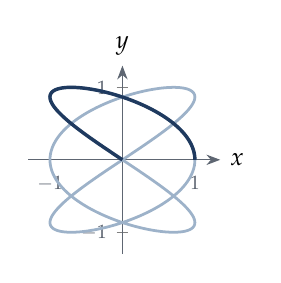
\begin{tikzpicture}
\begin{axis}[courbe,width=0.38\linewidth,xmin=-1.3,xmax=1.35,ymin=-1.3,ymax=1.3,xtick={-1,1},ytick={-1,1}]
\addplot[reste,domain=0:2*pi,samples=400]({cos(3*x)},{sin(2*x)});
\addplot[arcetude,domain=0:pi/2,samples=150]({cos(3*x)},{sin(2*x)});
\end{axis}
\end{tikzpicture}
\end{center}
\end{corrige}
\begin{corrige}{red-b}
Le domaine est $\R\setminus\big(\frac\pi2+\pi\Z\big)$ et $f$ est $2\pi$-périodique. Comme $f(t+\pi)=(\tan t,-\cos t)$, on
se ramène à $\left]-\frac\pi2,\frac\pi2\right[$ en complétant par la symétrie d'axe $(Ox)$. Comme $f(-t)=(-\tan t,\cos t)$,
on se ramène à $\left[0,\frac\pi2\right[$ en complétant par la symétrie d'axe $(Oy)$.
\end{corrige}
\begin{corrige}{red-c}
$x^2+y^2=(\cos t+\sin t)^2+(\cos t-\sin t)^2=2(\cos^2t+\sin^2t)=2$ : le support est inclus dans le cercle de centre $O$
et de rayon $\sqrt2$. Plus précisément, avec $\theta=t-\frac\pi4$, on a $x=\sqrt2\cos\theta$ et
$y=\sqrt2\cos\left(\theta+\frac\pi2\right)=-\sqrt2\sin\theta$. Lorsque $t$ décrit $[0,2\pi]$, $M(t)$ parcourt une fois tout
le cercle, dans le sens indirect. Il est inutile de chercher des symétries : la courbe est entièrement connue.
\end{corrige}
\begin{corrige}{b-famille}
La matrice est $\begin{pmatrix}1&a&a^2\\a&1&a\\a^2&a&1\end{pmatrix}$. L'opération $L_1\leftarrow L_1-aL_2$, qui ne change
pas le déterminant, donne la première ligne $(1-a^2,\ 0,\ 0)$. En développant selon cette ligne :
\[\det=(1-a^2)\dt{1&a\\a&1}=(1-a^2)^2.\]
Les vecteurs forment une base si et seulement si $a\neq1$ et $a\neq-1$. Pour $a=1$, les trois vecteurs sont égaux ;
pour $a=-1$, $\ve u=\ve w=(1,-1,1)$.
\end{corrige}
\begin{corrige}{b-J}
\textbf{1.} $J+\lambda I_n$ a pour coefficients diagonaux $1+\lambda$ et pour autres coefficients $1$ : d'après la
proposition~\ref{prop:ab}, $\det(J+\lambda I_n)=D_n(1+\lambda,1)=(\lambda+n)\lambda^{n-1}$.

\textbf{2.} Elle est inversible si et seulement si $\lambda\neq0$ et $\lambda\neq-n$.

\textbf{3.} $\lambda=-1$ n'est égal ni à $0$ ni à $-n$ lorsque $n\geq2$ : $J-I_n$ est inversible, de déterminant
$(n-1)(-1)^{n-1}$. Pour $n=1$, $J-I_1=(0)$ ne l'est pas, ce qui explique l'hypothèse.
\end{corrige}
\begin{corrige}{b-cercle}
\textbf{1.} $x^2+y^2=\dfrac{4t^2+(1-t^2)^2}{(1+t^2)^2}=\dfrac{1+2t^2+t^4}{(1+t^2)^2}=1$.

\textbf{2.} Soit $(x,y)\in\mathcal C$ avec $y\neq-1$, et $t=\frac x{1+y}$. Alors
$1+t^2=\frac{(1+y)^2+x^2}{(1+y)^2}=\frac{1+2y+y^2+x^2}{(1+y)^2}=\frac{2(1+y)}{(1+y)^2}=\frac2{1+y}$, d'où
\[\frac{2t}{1+t^2}=\frac{2x}{1+y}\cdot\frac{1+y}2=x,\qquad\frac{1-t^2}{1+t^2}=\frac2{1+t^2}-1=(1+y)-1=y.\]
Le point $(x,y)$ est donc $M(t)$. Le point $(0,-1)$ n'est pas atteint, car $y(t)=-1$ imposerait $1-t^2=-1-t^2$ ; il est
la limite de $M(t)$ lorsque $t\to\pm\infty$.

\textbf{3.} En dérivant les quotients,
\[x'(t)=\frac{2(1+t^2)-4t^2}{(1+t^2)^2}=\frac{2(1-t^2)}{(1+t^2)^2},\qquad
y'(t)=\frac{-2t(1+t^2)-2t(1-t^2)}{(1+t^2)^2}=\frac{-4t}{(1+t^2)^2},\]
soit $f'(t)=\frac2{(1+t^2)^2}(1-t^2,-2t)$. Le vecteur $(1-t^2,-2t)$ n'est jamais nul (si $t=0$, sa première coordonnée
vaut $1$) : la courbe est régulière. Enfin $\vv{OM(t)}\cdot(1-t^2,-2t)=\frac{2t(1-t^2)-2t(1-t^2)}{1+t^2}=0$ : la tangente
est orthogonale au rayon, conformément à l'exercice~\ref{e:fv-norme}.
\end{corrige}

\subsection*{Chapitre 4 --- Approfondissement}
\addcontentsline{toc}{subsection}{Chapitre 4 --- Approfondissement}
\markboth{7\quad Corrigés --- Chapitre 4}{}
\begin{corrige}{geo-aire}
\textbf{1.} $\vv{AB}=(3,1)$, $\vv{AC}=(1,4)$, $\det=12-1=11$ : l'aire vaut $\frac{11}2$.
\textbf{2.} $\det(\vv{OA},\vv{OB},\vv{OC})=\dt{1&0&1\\0&2&1\\0&0&3}=6$ : le volume vaut $\frac66=1$.
\end{corrige}
\begin{corrige}{geo-cop}
$\vv{AB}=(-1,1,0)$, $\vv{AC}=(-1,0,1)$, $\vv{AD}=(0,1,-1)$. Par Sarrus,
$\dt{-1&-1&0\\1&0&1\\0&1&-1}=(0+0+0)-(0-1+1)=0$. Les quatre points sont coplanaires ; en effet $D$ vérifie
$x+y+z=1$, l'équation du plan $(ABC)$ trouvée dans le cours.
\end{corrige}
\begin{corrige}{b-plan}
\textbf{1.} $\vv{AB}=(1,-1,1)$ et $\vv{AC}=(-1,0,1)$ ne sont pas colinéaires (leurs coordonnées ne sont pas
proportionnelles), donc $A,B,C$ ne sont pas alignés. Pour $M(x,y,z)$, en développant selon la première colonne,
\[\dt{x-1&1&-1\\y-1&-1&0\\z&1&1}=(x-1)(-1)-(y-1)(2)+z(-1)=-(x+2y+z-3).\]
Le plan $(ABC)$ a pour équation $x+2y+z=3$ ; on vérifie que $A$, $B$, $C$ conviennent.

\textbf{2.} $1+0+2=3$ : $D$ appartient au plan.

\textbf{3.} $\det(\vv{OA},\vv{OB},\vv{OC})=\dt{1&2&0\\1&0&1\\0&1&1}=(0+0+0)-(0+1+2)=-3$ par Sarrus : le volume vaut
$\frac{|-3|}6=\frac12$.
\end{corrige}
\begin{corrige}{geo-sym}
Les opérations $C_2\leftarrow C_2-C_1$ et $C_3\leftarrow C_3-C_1$, suivies d'un développement selon la dernière
ligne, donnent
\[\dt{x&x'-x&x''-x\\y&y'-y&y''-y\\1&0&0}=\dt{x'-x&x''-x\\y'-y&y''-y}=\det\big(\vv{MM'},\vv{MM''}\big),\]
avec le signe $(-1)^{3+1}=+1$. Ce déterminant est nul si et seulement si $\vv{MM'}$ et $\vv{MM''}$ sont colinéaires,
c'est-à-dire si les trois points sont alignés.
\end{corrige}
\begin{corrige}{geo-droites}
Les vecteurs $\ve u$ et $\ve v$ ne sont pas colinéaires : les droites ne sont pas parallèles, et elles sont donc
sécantes si et seulement si elles sont coplanaires, c'est-à-dire si $\det(\vv{AB},\ve u,\ve v)=0$. Avec
$\vv{AB}=(-1,1,m)$ et un développement selon la première colonne,
\[\dt{-1&1&0\\1&1&1\\m&0&1}=-1\cdot1-1\cdot1+m\cdot1=m-2.\]
Les droites sont sécantes si et seulement si $m=2$. Pour l'intersection, on résout
$(1+t,t,0)=(0,1+s,2+s)$ : $t=-1$ et $s=-2$, d'où le point $(0,-1,0)$.
\end{corrige}
\begin{corrige}{geo-dist}
\demarche{deux droites non parallèles : la proposition~\ref{prop:dist-droites} donne la distance par un produit mixte ; les points $H$ et $K$ s'obtiennent par deux conditions d'orthogonalité.}
\textbf{1.} $\ve u\wedge\ve v=(1\cdot1-0\cdot1,\ 0\cdot0-1\cdot1,\ 1\cdot1-1\cdot0)=(1,-1,1)$, de norme $\sqrt3$ : les droites
ne sont pas parallèles. Avec $\vv{AC_m}=(-1,0,m)$,
\[\det(\vv{AC_m},\ve u,\ve v)=(\ve u\wedge\ve v)\cdot\vv{AC_m}=-1+m,\qquad
d(\mathcal D_1,\mathcal D_m)=\frac{|m-1|}{\sqrt3}.\]
Les droites sont sécantes si et seulement si cette distance est nulle, c'est-à-dire $m=1$ (elles sont alors coplanaires et
non parallèles).

\textbf{2.} On cherche $H=A+s\ve u=(1+s,s,0)$ et $K=C_2+r\ve v=(0,r,2+r)$, avec $\vv{HK}=(-1-s,\ r-s,\ 2+r)$ orthogonal à
$\ve u$ et à $\ve v$ :
\[\vv{HK}\cdot\ve u=-1-2s+r=0,\qquad\vv{HK}\cdot\ve v=2r-s+2=0.\]
D'où $s=-\frac43$, $r=-\frac53$, $H=\left(-\frac13,-\frac43,0\right)$, $K=\left(0,-\frac53,\frac13\right)$ et
$\vv{HK}=\frac13(1,-1,1)$, colinéaire à $\ve u\wedge\ve v$, de norme $\frac{\sqrt3}3=\frac1{\sqrt3}$ : c'est bien
$d(\mathcal D_1,\mathcal D_2)$.
\end{corrige}
\begin{corrige}{g-antisym}
Si $A\in\mathcal M_{2p+1}(\R)$ vérifie $A^T=-A$, alors $\det A=\det(A^T)=\det(-A)=(-1)^{2p+1}\det A=-\det A$, donc
$\det A=0$ et $A$ n'est pas inversible.
\end{corrige}
\begin{corrige}{g-carre}
$(\det A)^2=\det(A^2)=\det(-I_n)=(-1)^n$. Or $\det A$ est réel, donc $(\det A)^2\geq0$ et $(-1)^n=1$ : $n$ est pair.
Pour une matrice complexe, l'argument tombe, car un carré complexe peut valoir $-1$ : $A=iI_n$ vérifie $A^2=-I_n$
pour tout $n$.
\end{corrige}
\begin{corrige}{f-transp}
\emph{Cas $n=2$.} Dans la base $(E_{1,1},E_{2,2},E_{1,2},E_{2,1})$, $T$ fixe les deux premières matrices et échange les
deux dernières. Sa matrice a pour colonnes $(1,0,0,0)$, $(0,1,0,0)$, $(0,0,0,1)$, $(0,0,1,0)$ : c'est $I_4$ dont on a
échangé les deux dernières colonnes, donc $\det T=-1$.

\emph{Cas général.} Prenons une base de $\Mn{\R}$ formée d'une base de $\mathcal S_n(\R)$ suivie d'une base de
$\mathcal A_n(\R)$. Comme $T(S)=S$ pour $S$ symétrique et $T(A)=-A$ pour $A$ antisymétrique, la matrice de $T$ dans
cette base est diagonale, avec $\frac{n(n+1)}2$ coefficients égaux à $1$ puis $\frac{n(n-1)}2$ égaux à $-1$. Ainsi
$\det T=(-1)^{n(n-1)/2}$, ce qui redonne $-1$ pour $n=2$.
\end{corrige}
\begin{corrige}{b-endo}
\textbf{1.} On calcule $AE_{1,1}=\begin{pmatrix}a&0\\c&0\end{pmatrix}$, $AE_{2,1}=\begin{pmatrix}b&0\\d&0\end{pmatrix}$,
$AE_{1,2}=\begin{pmatrix}0&a\\0&c\end{pmatrix}$, $AE_{2,2}=\begin{pmatrix}0&b\\0&d\end{pmatrix}$. Dans la base
$(E_{1,1},E_{2,1},E_{1,2},E_{2,2})$, la matrice de $f$ est
\[F=\begin{pmatrix}a&b&0&0\\c&d&0&0\\0&0&a&b\\0&0&c&d\end{pmatrix}.\]
\textbf{2.} En développant selon la première colonne,
\[\det F=a\dt{d&0&0\\0&a&b\\0&c&d}-c\dt{b&0&0\\0&a&b\\0&c&d}=a\,d\,(ad-bc)-c\,b\,(ad-bc)=(ad-bc)^2,\]
chaque déterminant de taille $3$ étant développé selon sa première ligne.

\textbf{3.} $f$ est bijectif si et seulement si $\det A\neq0$, c'est-à-dire si $A$ est inversible. C'est naturel :
si $A$ est inversible, $M\mapsto A^{-1}M$ est la réciproque de $f$ ; sinon, il existe une colonne $X\neq0$ telle que
$AX=0$, et la matrice $M$ dont les deux colonnes valent $X$ vérifie $f(M)=0$.
\end{corrige}
\begin{corrige}{g-proj}
\demarche{pour un endomorphisme défini géométriquement, on choisit la base où sa matrice est la plus simple (proposition~\ref{prop:proj-sym}).}
\textbf{1.} Dans une base adaptée à $E=\mathrm{Im}\,p\oplus\mathrm{Ker}\,p$, la matrice de $p$ est
$\mathrm{diag}(1,\dots,1,0,\dots,0)$ avec $r$ coefficients $1$ ; celle de $p+\lambda\Id$ est
$\mathrm{diag}(1+\lambda,\dots,1+\lambda,\lambda,\dots,\lambda)$, d'où
\[\det(p+\lambda\Id)=(1+\lambda)^r\lambda^{n-r}.\]
C'est un automorphisme si et seulement si ce déterminant est non nul : $\lambda\neq-1$ (si $r\geq1$) et $\lambda\neq0$ (si
$r\leq n-1$).

\textbf{2.} $s^2=4p^2-4p+\Id=\Id$ car $p^2=p$ : $s$ est une symétrie. Par la question 1 avec $\lambda=-\frac12$ :
$\det s=2^n\det\left(p-\frac12\Id\right)=2^n\left(\frac12\right)^r\left(-\frac12\right)^{n-r}=(-1)^{n-r}$. Par la
proposition~\ref{prop:proj-sym} : $s$ est la symétrie par rapport à $\mathrm{Im}\,p$ parallèlement à $\mathrm{Ker}\,p$, et
$\dim\mathrm{Ker}(s+\Id)=\dim\mathrm{Ker}\,p=n-r$.

\textbf{3.} $\det(A)^2=\det(A^2)=\det A$, donc $\det A\in\{0,1\}$. Si $\det A\neq0$, $A$ est inversible et, en multipliant
$A^2=A$ par $A^{-1}$, on obtient $A=I_n$, exclu. Donc $\det A=0$. Cette méthode n'utilise que la multiplicativité ; elle
est souvent la plus rapide.
\end{corrige}
\begin{corrige}{g-simil}
\demarche{on écrit la matrice en calculant l'image de chaque vecteur de la base $(1,i)$ ; la trace et le déterminant se lisent alors directement.}
\emph{Le mot « similitude » est hors programme ; l'exercice n'utilise que des outils du programme.}

\textbf{1.} $f(1)=a=\alpha+i\beta$ et $f(i)=ia=-\beta+i\alpha$ : la matrice est
$\begin{pmatrix}\alpha&-\beta\\\beta&\alpha\end{pmatrix}$, d'où $\mathrm{tr}\,f=2\alpha=2\,\mathrm{Re}(a)$ et
$\det f=\alpha^2+\beta^2=|a|^2\neq0$ : $f$ est bijective, et $f^{-1}:z\mapsto\frac1az$. $f$ est une symétrie si et
seulement si $f\circ f=\Id$, c'est-à-dire $a^2=1$ : $a=1$ ($f=\Id$) ou $a=-1$ ($f=-\Id$, symétrie centrale). Si $|a|=1$,
$a=e^{i\theta}$ et $f$ est la rotation de centre $O$ et d'angle $\theta$ ; sa matrice est
$\begin{pmatrix}\cos\theta&-\sin\theta\\\sin\theta&\cos\theta\end{pmatrix}$.

\textbf{2.} Pour $z,z'\in\C$ et $\lambda\in\R$, $\overline{z+\lambda z'}=\overline z+\lambda\overline{z'}$ car $\lambda$ est
réel : $g$ est $\R$-linéaire (mais pas $\C$-linéaire). $g(1)=a=(\alpha,\beta)$ et $g(i)=-ia=\beta-i\alpha=(\beta,-\alpha)$ :
\[\mathrm{Mat}(g)=\begin{pmatrix}\alpha&\beta\\\beta&-\alpha\end{pmatrix},\qquad\mathrm{tr}\,g=0,\qquad
\det g=-\alpha^2-\beta^2=-|a|^2.\]
Enfin $g(g(z))=a\,\overline{a\overline z}=a\overline a z=|a|^2z$ : $g\circ g=|a|^2\Id$.

\textbf{3.} $g$ est une symétrie si et seulement si $|a|^2=1$. Pour $a=e^{i\varphi}$ et $z=re^{i\psi}$ ($r>0$) :
$g(z)=re^{i(\varphi-\psi)}$, donc $g(z)=z\iff\psi\equiv\frac\varphi2\ [\pi]$ et $g(z)=-z\iff\psi\equiv\frac\varphi2+\frac\pi2\ [\pi]$.
$g$ est la symétrie par rapport à la droite d'angle $\frac\varphi2$, parallèlement à la droite perpendiculaire : c'est une
réflexion.

\textbf{4.} $\det f>0$ : $f$ conserve l'orientation (une base directe reste directe) ; $\det g<0$ : $g$ la renverse,
comme toute réflexion. On retrouve l'interprétation de l'étape 1 : le signe du déterminant est celui de l'aire orientée.
\end{corrige}
\begin{corrige}{hp-com}
\demarche{on applique la formule de l'encadré hors programme du chapitre 1 ; les questions théoriques reposent sur $A\,\mathrm{com}(A)^T=\det(A)I_n$ et sur la multiplicativité.}
\textbf{1.} En développant selon la première ligne, $\det A=1\cdot1-2\cdot(0-1)+0=3$. Les cofacteurs
$(-1)^{i+j}\Delta_{i,j}$ sont, ligne par ligne :
\[\mathrm{com}(A)=\begin{pmatrix}1&1&-1\\-2&1&2\\2&-1&1\end{pmatrix},\qquad
A\,\mathrm{com}(A)^T=\begin{pmatrix}1&2&0\\0&1&1\\1&0&1\end{pmatrix}\begin{pmatrix}1&-2&2\\1&1&-1\\-1&2&1\end{pmatrix}=3I_3,\]
donc $A^{-1}=\frac13\begin{pmatrix}1&-2&2\\1&1&-1\\-1&2&1\end{pmatrix}$.

\textbf{2.} Si $\det A=\pm1$, $A^{-1}=\pm\mathrm{com}(A)^T$, et les cofacteurs, déterminants de matrices à coefficients
entiers, sont entiers. Réciproquement, si $A$ et $A^{-1}$ sont à coefficients entiers, leurs déterminants sont des entiers
de produit $\det(AA^{-1})=1$ : ils valent $\pm1$.

\textbf{3.} En prenant le déterminant de $A\,\mathrm{com}(A)^T=\det(A)\,I_n$ : $\det A\cdot\det\mathrm{com}(A)=(\det A)^n$,
d'où $\det\big(\mathrm{com}(A)\big)=(\det A)^{n-1}$.
\end{corrige}
\begin{corrige}{v-calc}
\emph{Par la méthode~\ref{meth:poly}.} La variable n'apparaît que dans la première colonne ; en développant selon
elle, $P$ est de degré au plus $2$, et le coefficient de $x^2$ est le cofacteur de la position $(3,1)$, soit
$+\dt{1&1\\2&3}=1$. Pour $x=2$, la première colonne égale la deuxième ; pour $x=3$, la troisième. Donc
$P(x)=(x-2)(x-3)$.

\emph{Par Vandermonde.} $P(x)$ est le déterminant de la transposée de la matrice de Vandermonde de $(x,2,3)$ :
$P(x)=V(x,2,3)=(2-x)(3-x)(3-2)=(x-2)(x-3)$.
\end{corrige}
\begin{corrige}{b-vdm3}
\textbf{1.} $A$ est la matrice de Vandermonde de $(1,2,3)$ : $\det A=(2-1)(3-1)(3-2)=2\neq0$, donc $A$ est inversible.

\textbf{2.} $\det(2A^{-1}A^T)=2^3\cdot\frac12\cdot2=8$. Pour $\det(A^2-A^TA)$, aucune règle ne donne le déterminant
d'une \emph{différence} : il faut calculer la matrice. On a $A^2-A^TA=(A-A^T)A$, d'où
$\det(A^2-A^TA)=\det(A-A^T)\det A$. Or $A-A^T$ est antisymétrique d'ordre $3$, donc de déterminant nul
(exercice~\ref{e:g-antisym}). Ainsi $\det(A^2-A^TA)=0$. La factorisation à droite par $A$ était la clé.
\end{corrige}
\begin{corrige}{v-lagrange}
Écrivons $L=c_0+c_1X+\dots+c_{n-1}X^{n-1}$. Les conditions $L(x_i)=y_i$ forment le système
$\sum_{j=0}^{n-1}c_jx_i^{\,j}=y_i$, c'est-à-dire $VC=Y$, où $V=(x_i^{\,j-1})_{i,j}$ est la matrice de Vandermonde des
$x_i$. Ceux-ci étant distincts, $\det V\neq0$ : $V$ est inversible et le système possède une unique solution,
d'après la caractérisation des matrices inversibles (étape 4). Il existe donc un unique polynôme $L$ convenable.
\end{corrige}
\begin{corrige}{v-exp}
\textbf{1.} Supposons $\lambda e^x+\mu e^{2x}=0$ pour tout $x$. En $x=0$ : $\lambda+\mu=0$. En dérivant puis en
évaluant en $0$ : $\lambda+2\mu=0$. Le déterminant de ce système est $\dt{1&1\\1&2}=1\neq0$, donc $\lambda=\mu=0$.

\textbf{2.} Supposons $\sum_i\lambda_ie^{\alpha_ix}=0$ pour tout $x$. En dérivant $k$ fois puis en évaluant en $0$, on
obtient $\sum_i\lambda_i\alpha_i^{\,k}=0$ pour $k\in\ient0{n-1}$. Ce système a pour matrice la transposée de la matrice
de Vandermonde des $\alpha_i$, de déterminant non nul puisque les $\alpha_i$ sont distincts : $\lambda_1=\dots=\lambda_n=0$.
\end{corrige}
\begin{corrige}{b-eval}
\textbf{1.} Pour $P,Q$ et $\lambda$, $(\lambda P+Q)(k)=\lambda P(k)+Q(k)$ : $\varphi$ est linéaire. L'image de $X^j$ est
$(0^j,1^j,\dots,n^j)$ (avec $0^0=1$), donc $M=(i^{\,j})_{0\leq i,j\leq n}$ : c'est la matrice de Vandermonde de
$(0,1,\dots,n)$.

\textbf{2.} $\det M=\prod_{0\leq i<j\leq n}(j-i)$. Pour $j$ fixé, $\prod_{i<j}(j-i)=j\times(j-1)\times\dots\times1=j!$,
donc $\det M=\prod_{j=1}^nj!\neq0$. Ainsi $M$ est inversible et $\varphi$ est un isomorphisme (les deux espaces ont la
même dimension $n+1$).

\textbf{3.} Pour toutes valeurs $y_0,\dots,y_n$, il existe un unique polynôme de degré au plus $n$ prenant ces valeurs
en $0,1,\dots,n$ : c'est le cas particulier de l'exercice~\ref{e:v-lagrange} pour les points $0,1,\dots,n$.
\end{corrige}
\begin{corrige}{b-poly}
\emph{Cas $n=2$.} $X^2$, $(X+1)^2=1+2X+X^2$ et $(X-1)^2=1-2X+X^2$ ont pour coordonnées dans $(1,X,X^2)$ les colonnes
de $\begin{pmatrix}0&1&1\\0&2&-2\\1&1&1\end{pmatrix}$, dont le déterminant vaut, selon la première colonne,
$1\times\dt{1&1\\2&-2}=-4\neq0$ : c'est une base.

\emph{Cas général.} La famille comporte $n+1=\dim\K_n[X]$ vecteurs ; il suffit de montrer que son déterminant dans la
base $(1,X,\dots,X^n)$ est non nul. D'après la formule du binôme, $(X+a_i)^n=\sum_{k=0}^n\binom nk a_i^{\,n-k}X^k$ :
la matrice $M$ des coordonnées a pour coefficient, en ligne $k$ et colonne $i$, le nombre $\binom nk a_i^{\,n-k}$.
En factorisant $\binom nk$ dans chaque ligne,
\[\det M=\Big(\prod_{k=0}^n\binom nk\Big)\det\big(a_i^{\,n-k}\big)_{k,i}.\]
La dernière matrice est la transposée d'une matrice de Vandermonde dont on a renversé l'ordre des lignes ; son
déterminant vaut $\pm V(a_0,\dots,a_n)$, qui est non nul. La famille est donc une base.
\end{corrige}
\begin{corrige}{r-gen}
On développe selon la première ligne, qui ne contient que $a$ (position $(1,1)$) et $b$ (position $(1,2)$) :
$T_n=aT_{n-1}-b\,M$, où $M$ est obtenu en rayant la ligne $1$ et la colonne $2$. La première colonne de $M$ est
$(c,0,\dots,0)^T$ ; en la développant, $M=c\,T_{n-2}$. Donc $T_n=aT_{n-1}-bc\,T_{n-2}$. Avec $a=2$ et $b=c=-1$, on a
$bc=1$ et l'on retrouve $\Delta_n=2\Delta_{n-1}-\Delta_{n-2}$.
\end{corrige}
\begin{corrige}{b-period}
\textbf{1.} $T_1=1$, $T_2=\dt{1&1\\1&1}=0$, $T_3=\dt{1&1&0\\1&1&1\\0&1&1}=1\cdot0-1\cdot1+0=-1$.

\textbf{2.} D'après l'exercice~\ref{e:r-gen} avec $a=b=c=1$ : $T_n=T_{n-1}-T_{n-2}$.

\textbf{3.} On calcule de proche en proche : $T_1=1$, $T_2=0$, $T_3=-1$, $T_4=-1$, $T_5=0$, $T_6=1$, $T_7=1$, $T_8=0$.
Comme $(T_7,T_8)=(T_1,T_2)$ et que chaque terme ne dépend que des deux précédents, la suite est $6$-périodique.
Comme $100=6\times16+4$, $T_{100}=T_4=-1$.
\end{corrige}
\begin{corrige}{r-ab}
D'après l'exercice~\ref{e:r-gen}, avec $a+b$ sur la diagonale et un produit $ab\times1=ab$ des coefficients voisins, on a $D_n=(a+b)D_{n-1}-ab\,D_{n-2}$ pour $n\geq3$,
avec $D_1=a+b$ et $D_2=(a+b)^2-ab=a^2+ab+b^2$. En posant $D_0=1$, la relation reste vraie pour $n=2$.

L'équation caractéristique $r^2-(a+b)r+ab=(r-a)(r-b)=0$ a deux racines distinctes, donc $D_n=\lambda a^n+\mu b^n$.
Les conditions $\lambda+\mu=1$ et $\lambda a+\mu b=a+b$ donnent $\lambda=\frac{a}{a-b}$ et $\mu=-\frac{b}{a-b}$, d'où
\[D_n=\frac{a^{n+1}-b^{n+1}}{a-b}=a^n+a^{n-1}b+\dots+b^n.\]
On contrôle : $D_1=a+b$ et $D_2=a^2+ab+b^2$. Lorsque $a=b$, la racine est double et l'on trouve $D_n=(n+1)a^n$, ce
qui généralise l'exemple~\ref{ex:tridiag}.
\end{corrige}
\begin{corrige}{r-321}
\demarche{déterminant tridiagonal : on applique la méthode~\ref{meth:rec}, ou directement l'exercice~\ref{e:r-gen}.}
$T_1=3$, $T_2=9-2=7$ et, pour $n\geq3$, $T_n=3T_{n-1}-2T_{n-2}$ (exercice~\ref{e:r-gen} avec $a=3$, $bc=2$).
L'équation caractéristique $r^2-3r+2=0$ a pour racines $1$ et $2$ : $T_n=\alpha+\beta2^n$. Les conditions $\alpha+2\beta=3$,
$\alpha+4\beta=7$ donnent $\beta=2$, $\alpha=-1$ : $T_n=2^{n+1}-1$. Vérification : $T_3=3\cdot7-2\cdot3=15$. (Le TD traite
de même $5$, $6$, $1$, avec les racines $2$ et $3$ : $3^{n+1}-2^{n+1}$.)
\end{corrige}
\begin{corrige}{r-x}
\demarche{récurrence d'ordre 2 dont les racines dépendent de $x$ : on distingue le cas de la racine double.}
$T_1=1+x^2$, $T_2=(1+x^2)^2-x^2=1+x^2+x^4$, et $T_n=(1+x^2)T_{n-1}-x^2T_{n-2}$. L'équation $r^2-(1+x^2)r+x^2=0$ a pour
racines $1$ et $x^2$.
\begin{itemize}
\item Si $x^2\neq1$ : $T_n=\alpha+\beta x^{2n}$, et les conditions initiales (en posant $T_0=1$, compatible avec la
      relation pour $n=2$) donnent $T_n=\dfrac{1-x^{2n+2}}{1-x^2}=1+x^2+\dots+x^{2n}$.
\item Si $x^2=1$ : racine double $1$, $T_n=\alpha+\beta n$ avec $T_0=1$, $T_1=2$ : $T_n=n+1$, ce que donne aussi la somme
      précédente.
\end{itemize}
Pour $x=-1$, on retrouve le déterminant de l'exemple~\ref{ex:tridiag} ($2$ sur la diagonale, $-1$ à côté) : $n+1$.
\end{corrige}
\begin{corrige}{r-cheb}
\demarche{la relation de récurrence est celle de l'exercice~\ref{e:r-gen} ; on vérifie la formule par récurrence avec une formule de trigonométrie, puis on compte les racines.}
\textbf{1.} $D_1=2\cos\theta=\frac{\sin2\theta}{\sin\theta}$, $D_2=4\cos^2\theta-1=\frac{\sin3\theta}{\sin\theta}$ (car
$\sin3\theta=\sin\theta(4\cos^2\theta-1)$), et $D_n=2\cos\theta\,D_{n-1}-D_{n-2}$. Or
$\sin\big((n+1)\theta\big)+\sin\big((n-1)\theta\big)=2\sin(n\theta)\cos\theta$ ; si la formule est vraie aux rangs $n-1$
et $n-2$, elle l'est donc au rang $n$. (On peut aussi résoudre la récurrence : l'équation caractéristique
$r^2-2\cos\theta\,r+1=0$ a pour racines $e^{\pm i\theta}$.)

\textbf{2.} $D_n=0\iff\sin\big((n+1)\theta\big)=0\iff\theta=\frac{k\pi}{n+1}$, avec $1\leq k\leq n$ pour rester dans
$]0,\pi[$.

\textbf{3.} En développant selon la première ligne, $P_n(x)=xP_{n-1}(x)-P_{n-2}(x)$ : par récurrence, $P_n$ est un polynôme
de degré $n$, de coefficient dominant $1$. D'après la question 2, $P_n\big(2\cos\frac{k\pi}{n+1}\big)=0$ pour
$1\leq k\leq n$ ; ces $n$ réels sont distincts (le cosinus est injectif sur $]0,\pi[$). Un polynôme de degré $n$ ayant $n$
racines distinctes n'en a pas d'autre : les racines de $P_n$ sont exactement les $2\cos\frac{k\pi}{n+1}$, et
$P_n(x)=\prod_{k=1}^n\left(x-2\cos\frac{k\pi}{n+1}\right)$.
\end{corrige}
\begin{corrige}{f-min}
\demarche{les colonnes voisines diffèrent peu : on les soustrait en partant de la dernière (méthode~\ref{meth:diff}).}
Pour $k$ de $n$ à $2$, $C_k\leftarrow C_k-C_{k-1}$. Le coefficient $(i,k)$ devient $\min(i,k)-\min(i,k-1)$, qui vaut $0$
si $i\leq k-1$ et $1$ si $i\geq k$. La matrice obtenue est triangulaire inférieure, à diagonale de $1$ (la première
colonne est formée de $1$) : le déterminant vaut $1$.
\end{corrige}
\begin{corrige}{f-absij}
\demarche{comme pour $\max(i,j)$, on soustrait les colonnes voisines ; une seconde vague d'opérations, sur les lignes, isole ensuite les coefficients.}
\etape{Colonnes} Pour $k$ de $n$ à $2$, $C_k\leftarrow C_k-C_{k-1}$ : le coefficient $(i,k)$ devient $|i-k|-|i-k+1|$,
égal à $1$ si $i\leq k-1$ et à $-1$ si $i\geq k$. La première colonne reste $(0,1,\dots,n-1)^T$.
\etape{Lignes} Pour $i$ de $n$ à $2$, $L_i\leftarrow L_i-L_{i-1}$ : la ligne $i$ devient
$(1,0,\dots,0,-2,0,\dots,0)$, le $-2$ étant en colonne $i$ ; la ligne $1$ reste $(0,1,\dots,1)$.
\etape{Conclure} $C_1\leftarrow C_1+\frac12(C_2+\dots+C_n)$ annule la première colonne sauf son premier coefficient,
égal à $\frac{n-1}2$. La matrice est triangulaire supérieure de diagonale $\left(\frac{n-1}2,-2,\dots,-2\right)$ :
\[B_n=\frac{n-1}2(-2)^{n-1}=(-1)^{n-1}(n-1)\,2^{n-2}.\]
Vérification : $B_2=\dt{0&1\\1&0}=-1$ et $B_3=4$.
\end{corrige}
\begin{corrige}{f-ipj}
\demarche{avant toute opération, on se demande si les colonnes ne sont pas liées.}
La colonne $j$ s'écrit $(i)_i+j\,(1)_i=V+jU$ avec $V=(1,2,\dots,n)^T$ et $U=(1,\dots,1)^T$ : toutes les colonnes sont dans
$\vect(U,V)$, de dimension au plus $2$. Pour $n\geq3$, les colonnes sont liées et le déterminant est nul. Pour $n=1$, il vaut
$2$ ; pour $n=2$, $\dt{2&3\\3&4}=-1$. La méthode des différences aurait aussi conclu ($C_3-C_2=C_2-C_1$), mais repérer le rang
est immédiat.
\end{corrige}
\begin{corrige}{f-ka}
\demarche{la colonne $k$ « ressemble » à la colonne $k-1$ multipliée par $a$ au-dessus de la diagonale : on retranche $aC_{k-1}$ pour y créer des zéros.}
Pour $k$ de $n$ à $2$, $C_k\leftarrow C_k-aC_{k-1}$. Le coefficient $(i,k)$ devient $a^{|i-k|}-a\cdot a^{|i-k+1|}$.
\begin{itemize}
\item Si $i\leq k-1$ : $a^{k-i}-a\cdot a^{k-1-i}=0$.
\item Si $i\geq k$ : $a^{i-k}-a\cdot a^{i-k+1}=a^{i-k}(1-a^2)$.
\end{itemize}
La matrice est triangulaire inférieure, de diagonale $(1,1-a^2,\dots,1-a^2)$ : le déterminant vaut $(1-a^2)^{n-1}$. Il
est nul si et seulement si $a=\pm1$, ce qui se voit aussi directement : pour $a=1$ toutes les colonnes sont égales, pour
$a=-1$ elles sont opposées deux à deux.
\end{corrige}
\begin{corrige}{x-gen}
\demarche{on reprend l'une des deux méthodes de l'exemple~\ref{ex:X} ; la permutation simultanée des lignes et des colonnes est la plus rapide.}
\textbf{1.} On réordonne lignes et colonnes \emph{par la même permutation} $1,2n,2,2n-1,\dots,n,n+1$ ; le déterminant ne
change pas (les deux signes se compensent). La matrice devient diagonale par blocs, de blocs
$\begin{pmatrix}a_i&b_i\\b_{2n+1-i}&a_{2n+1-i}\end{pmatrix}$, d'où le produit annoncé. (Par récurrence : développer selon la
première ligne puis selon la dernière donne $D_{2n}=(a_1a_{2n}-b_1b_{2n})D_{2n-2}$, comme dans l'exemple.)

\textbf{2.} Le coefficient central $c$ est le seul non nul de sa ligne et de sa colonne $n+1$ ; on développe selon cette
ligne (signe $(-1)^{2(n+1)}=+1$) et l'on se ramène à la question 1 : $D=c\prod_{i=1}^n(a_ia_{2n+2-i}-b_ib_{2n+2-i})$.

\textbf{3.} Avec $n=2$, $a_i=x$, $b_i=1$, $c=x$ : $D=x(x^2-1)^2$. La matrice est inversible si et seulement si
$x\notin\{-1,0,1\}$.
\end{corrige}
\begin{corrige}{lettres}
\demarche{des lignes (ou colonnes) qui ne contiennent qu'un coefficient : on développe selon elles l'une après l'autre, en suivant les signes.}
\textbf{1.} Pour $2\leq j\leq n-1$, la colonne $j$ ne contient que $b_j$, en position diagonale (signe $+$). En développant
successivement selon ces colonnes, il reste le déterminant des lignes et colonnes $1$ et $n$ :
\[D_N=b_2\cdots b_{n-1}\dt{a_1&c_1\\a_n&c_n}=b_2\cdots b_{n-1}\,(a_1c_n-a_nc_1).\]

\textbf{2.} Pour $2\leq k\leq n-1$, on sort $b_{n+1-k}$ de la ligne $k$, qui devient un vecteur de base $e_{n+1-k}^T$ ;
puis on retranche ces lignes, avec les bons coefficients, aux lignes $1$ et $n$ pour annuler les colonnes $2$ à $n-1$
(transvections). On obtient $b_2\cdots b_{n-1}$ fois le déterminant de la matrice dont les lignes $1$ et $n$ sont
$(a_1,0,\dots,0,a_n)$ et $(c_1,0,\dots,0,c_n)$, et dont les lignes $2$ à $n-1$ forment une « anti-identité » sur les
colonnes $2$ à $n-1$. Remettre ces $n-2$ lignes dans l'ordre demande $\left\lfloor\frac{n-2}2\right\rfloor$ échanges ; on se
ramène alors au cas 1 :
\[D_Z=(-1)^{\lfloor\frac{n-2}2\rfloor}\,b_2\cdots b_{n-1}\,(a_1c_n-a_nc_1).\]
Par exemple, en ordre $4$, $D_Z=-b_2b_3(a_1c_4-a_4c_1)$.
\end{corrige}
\begin{corrige}{cyc-base}
\demarche{« base ? » : on calcule le déterminant de la famille dans la base $(e_j)$ ; la première ligne n'a que deux coefficients non nuls.}
La matrice de la famille a des $1$ sur la diagonale, des $\lambda$ juste au-dessous, et un $\lambda$ en position $(1,n)$.
En développant selon la première ligne $(1,0,\dots,0,\lambda)$ :
\begin{itemize}
\item le mineur $\Delta_{1,1}$ est triangulaire inférieur à diagonale de $1$ : il vaut $1$ ;
\item le mineur $\Delta_{1,n}$ (lignes $2$ à $n$, colonnes $1$ à $n-1$) est triangulaire supérieur à diagonale de
      $\lambda$ : il vaut $\lambda^{n-1}$.
\end{itemize}
Donc $\det=1+(-1)^{1+n}\lambda\cdot\lambda^{n-1}=1-(-\lambda)^n$. La famille est une base si et seulement si
$(-\lambda)^n\neq1$, c'est-à-dire $\lambda\neq-1$, et de plus $\lambda\neq1$ lorsque $n$ est pair. Vérification pour $n=2$ :
$\dt{1&\lambda\\\lambda&1}=1-\lambda^2$.
\end{corrige}
\begin{corrige}{b-affine}
\textbf{1.} Notons $C_1,\dots,C_n$ les colonnes de $D$ et $U=(1,\dots,1)^T$ ; les colonnes de $D(x)$ sont les
$C_j+xU$. Les opérations $C_j\leftarrow C_j-C_1$ pour $j\geq2$ ne changent pas le déterminant et produisent des
colonnes $C_j-C_1$ indépendantes de $x$. Seule la première colonne $C_1+xU$ dépend encore de $x$, et par linéarité
par rapport à celle-ci,
\[D(x)=\det(C_1,C_2-C_1,\dots,C_n-C_1)+x\det(U,C_2-C_1,\dots,C_n-C_1)=\beta+\alpha x.\]

\textbf{2.} Pour $x=-b$, les coefficients situés au-dessus de la diagonale s'annulent : la matrice est triangulaire
inférieure de diagonale $(a_i-b)_i$, donc $D(-b)=P(b)$. De même, $D(-c)=P(c)$. On résout le système
$\beta-\alpha b=P(b)$, $\beta-\alpha c=P(c)$ ; en multipliant la première équation par $c$, la seconde par $b$ et en
soustrayant, on élimine $\alpha$ :
\[D=D(0)=\beta=\frac{c\,P(b)-b\,P(c)}{c-b}.\]

\textbf{3.} Pour $n=1$ : $\frac{c(a_1-b)-b(a_1-c)}{c-b}=\frac{a_1(c-b)}{c-b}=a_1$. Lorsque tous les $a_i$ valent $a$,
$P(x)=(a-x)^n$ et $D=\frac{c(a-b)^n-b(a-c)^n}{c-b}$. Lorsque $c\to b$, c'est un taux d'accroissement : en posant
$g(t)=t(a-b)^n-b(a-t)^n$, on a $D=\frac{g(c)-g(b)}{c-b}\to g'(b)=(a-b)^n+nb(a-b)^{n-1}=(a-b)^{n-1}\big(a+(n-1)b\big)$,
c'est-à-dire $D_n(a,b)$.
\end{corrige}
\begin{corrige}{b-affine-ab}
\demarche{la formule de l'exercice~\ref{e:b-affine} n'a pas de sens pour $b=c$ ; on la prolonge par continuité, et la limite obtenue est un taux d'accroissement.}
\textbf{1.} Notons $A(a,b)$ la matrice ayant $a$ au-dessus de la diagonale et $b$ au-dessous. Pour $b\neq a$,
l'exercice~\ref{e:b-affine} donne $\det A(a,b)=\frac{b\,P(a)-a\,P(b)}{b-a}$. Posons $\varphi(u)=u\,P(a)-a\,P(u)$ ; comme
$\varphi(a)=0$,
\[\det A(a,b)=\frac{\varphi(b)-\varphi(a)}{b-a}\xrightarrow[b\to a]{}\varphi'(a)=P(a)-aP'(a).\]
Or $b\mapsto\det A(a,b)$ est polynomiale (développement), donc continue : $\det A=\det A(a,a)=P(a)-aP'(a)$.

\textbf{2.} $P'(x)=-\sum_{j=1}^n\prod_{i\neq j}(\lambda_i-x)$, d'où
\[\det A=\prod_{i=1}^n(\lambda_i-a)+a\sum_{j=1}^n\prod_{i\neq j}(\lambda_i-a).\]
Pour $\lambda_i=i$ et $a=1$ : le produit contient le facteur $\lambda_1-1=0$, et dans la somme seul le terme $j=1$ est non
nul : $\det A=\prod_{i=2}^n(i-1)=(n-1)!$. Vérification pour $n=2$ : $\dt{1&1\\1&2}=1$.
\end{corrige}

\subsection*{Chapitre 5 --- Séance 2}
\addcontentsline{toc}{subsection}{Chapitre 5 --- Séance 2}
\markboth{7\quad Corrigés --- Chapitre 5}{}
\begin{corrige}{loc-a}
\demarche{regrouper le développement par puissances et s'arrêter au premier vecteur non colinéaire au premier.}
Pour $(t^3,t^5)$ : $f(h)=h^3(1,0)+h^5(0,1)$, donc $p=3$, $q=5$, tous deux impairs : point d'inflexion (stationnaire),
tangente horizontale. Pour $(t^2+t^3,t^3)$ : $f(h)=h^2(1,0)+h^3(1,1)$, donc $p=2$, $q=3$ : rebroussement de première
espèce, tangente horizontale.
\end{corrige}
\begin{corrige}{br-d}
\demarche{limites de $x$ et $y$, puis $y/x$, puis $y-ax$ ; on ne conclut qu'après le dernier calcul.}
\textbf{1.} $x$ et $y$ tendent vers $+\infty$ ; $\frac yx=1+\frac{\ln t}t\to1$ : direction asymptotique $y=x$. Mais
$y-x=\ln t\to+\infty$ : il n'y a pas d'asymptote, c'est une branche parabolique de direction $y=x$.

\textbf{2.} $x$ et $y$ tendent vers $+\infty$ ; $\frac yx=\frac{t+2+1/t^2}{t+1/t}\to1$. Puis
$y-x=2+\frac1{t^2}-\frac1t\to2$ : la droite $y=x+2$ est asymptote. Enfin $y-x-2=\frac1{t^2}-\frac1t=\frac{1-t}{t^2}<0$ pour
$t>1$ : la courbe est au-dessous de l'asymptote. Les deux questions montrent que seul le calcul de $\lim(y-ax)$ permet de
conclure.
\end{corrige}
\begin{corrige}{tp1}
\demarche{point singulier, donc développement limité ; la position se lit sur le terme en $t^3$, le sens sur la variation de $t^2$.}
$f'(t)=(2t+3t^2,\ 2t-3t^2)$ est nul en $0$ : $O$ est singulier. Ici le développement est exact :
$f(t)=t^2(1,1)+t^3(1,-1)$. Les vecteurs $\ve a=(1,1)$ et $\ve b=(1,-1)$ ne sont pas colinéaires : $p=2$, $q=3$,
rebroussement de première espèce, de tangente la droite $y=x$.

\emph{Décisions de tracé.} Pour $t$ petit, $M(t)$ est proche du point $t^2(1,1)$ de la demi-droite $y=x$, $x>0$ : la
courbe arrive en $O$ \emph{et en repart} le long de cette demi-droite. Le terme $t^3(1,-1)$ indique le côté : pour $t<0$, la
courbe est du côté de $-\ve b$, au-dessus de la tangente ; pour $t>0$, du côté de $\ve b$, au-dessous. Comme $t^2$ décroît
pour $t<0$ et croît pour $t>0$, le point arrive en $O$ par l'arc supérieur et repart par l'arc inférieur.
\begin{center}
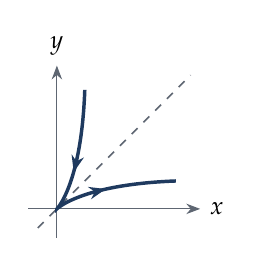
\begin{tikzpicture}
\begin{axis}[courbe,width=0.36\linewidth,xmin=-0.15,xmax=0.75,ymin=-0.15,ymax=0.75,xtick=\empty,ytick=\empty]
\addplot[asy,domain=-0.1:0.7,samples=2]{x};
\addplot[arcetude,domain=-0.62:0.62,samples=200]({x^2+x^3},{x^2-x^3});
\draw[-{Stealth[length=6pt]},Bleu,line width=1.2pt] (axis cs:0.096,0.224)--(axis cs:0.088,0.192);
\draw[-{Stealth[length=6pt]},Bleu,line width=1.2pt] (axis cs:0.224,0.096)--(axis cs:0.256,0.104);
\end{axis}
\end{tikzpicture}
\end{center}
\end{corrige}

\subsection*{Chapitre 5 --- Exercices de tracé}
\addcontentsline{toc}{subsection}{Chapitre 5 --- Exercices de tracé}
\markboth{7\quad Corrigés --- Chapitre 5}{}
\begin{corrige}{loc-b}
$f'(t)=(e^t-1,3t^2)$ est nul en $0$. Avec $e^h=1+h+\frac{h^2}2+\frac{h^3}6+o(h^3)$ :
$f(h)=(1,0)+h^2\left(\tfrac12,0\right)+h^3\left(\tfrac16,1\right)+o(h^3)$. Les vecteurs $\left(\frac12,0\right)$ et
$\left(\frac16,1\right)$ ne sont pas colinéaires : $p=2$, $q=3$, rebroussement de première espèce en $(1,0)$, à tangente
horizontale.
\end{corrige}
\begin{corrige}{loc-c}
On pose $t=1+h$. D'une part $\frac1{1+h}=1-h+h^2-h^3+o(h^3)$, donc $x=2+h^2-h^3+o(h^3)$. D'autre part
$(1+h)\ln(1+h)=(1+h)\left(h-\frac{h^2}2+\frac{h^3}3\right)+o(h^3)=h+\frac{h^2}2-\frac{h^3}6+o(h^3)$, donc
$y=-1+\frac{h^2}2-\frac{h^3}6+o(h^3)$. Ainsi
\[f(1+h)=(2,-1)+h^2\left(1,\tfrac12\right)+h^3\left(-1,-\tfrac16\right)+o(h^3).\]
Le déterminant $\dt{1&-1\\\frac12&-\frac16}=-\frac16+\frac12=\frac13$ est non nul : les vecteurs ne sont pas colinéaires,
$p=2$, $q=3$. Le point $M(1)=(2,-1)$ est un rebroussement de première espèce, de tangente dirigée par $(2,1)$.
\end{corrige}
\begin{corrige}{loc-d}
On a $f'(t)=(-\sin t,3\sin^2t\cos t)$ et $f''(t)=(-\cos t,6\sin t\cos^2t-3\sin^3t)$, donc
\begin{align*}
\det\big(f'(t),f''(t)\big)&=-\sin t\,(6\sin t\cos^2t-3\sin^3t)+3\sin^2t\cos^2t\\
&=3\sin^2t\,(\sin^2t-\cos^2t)=-3\sin^2t\cos2t.
\end{align*}
Ce déterminant s'annule pour $t\in\{-\pi,0,\pi\}$, valeurs qui correspondent aux points stationnaires (étudiés à
l'exemple~\ref{ex:cos-sin3}), et pour $t\in\left\{\pm\frac\pi4,\pm\frac{3\pi}4\right\}$, où $\cos2t=0$. En ces quatre
dernières valeurs, $\sin t\neq0$ : le point est régulier, et $\cos2t$ change de signe. Ce sont des points
d'inflexion, de coordonnées $\left(\pm\frac{\sqrt2}2,\pm\frac{\sqrt2}4\right)$.
\end{corrige}
\begin{corrige}{br-b}
$f'(t)=(e^t,2t)$ ne s'annule pas : la courbe est régulière. Avec $f''(t)=(e^t,2)$,
$\det\big(f'(t),f''(t)\big)=2e^t-2te^t=2e^t(1-t)$, qui s'annule en changeant de signe pour $t=1$ : le point
$M(1)=(e,1)$ est un point d'inflexion.

Lorsque $t\to+\infty$, $x$ et $y$ tendent vers $+\infty$ et $\frac yx=t^2e^{-t}\to0$ par croissances comparées :
branche parabolique de direction $(Ox)$. Lorsque $t\to-\infty$, $x\to0$ et $y\to+\infty$ : la droite $x=0$ est
asymptote verticale. Le support est le graphe de $x\mapsto(\ln x)^2$ sur $\R_+^*$, dont la dérivée seconde
$\frac{2(1-\ln x)}{x^2}$ s'annule bien en $x=e$ en changeant de signe.
\end{corrige}
\begin{corrige}{br-c}
\demarche{on commence par les limites de $x$ et $y$ aux bornes : une limite infinie annonce une branche infinie, une limite finie un point limite.}
\textbf{1.} Lorsque $t\to0$, $x$ et $y$ tendent vers l'infini, avec le signe de $t$. Comme $e^t-1\sim t$,
$\frac yx=\frac t{e^t-1}\to1$. Pour étudier $y-x$, on écrit $e^t-1=t\left(1+\frac t2+\frac{t^2}6+o(t^2)\right)$ et l'on
utilise $\frac1{1+u}=1-u+u^2+o(u^2)$ :
\[y=\frac1t\left(1-\tfrac t2-\tfrac{t^2}6+\tfrac{t^2}4+o(t^2)\right)=\frac1t-\frac12+\frac t{12}+o(t).\]
Ainsi $y-x=-\frac12+\frac{t}{12}+o(t)$ : la droite $\mathcal A:y=x-\frac12$ est asymptote, et
$y-\left(x-\frac12\right)\sim\frac t{12}$ : la courbe est au-dessus de $\mathcal A$ lorsque $t\to0^+$ (côté
$x\to+\infty$) et au-dessous lorsque $t\to0^-$ (côté $x\to-\infty$).

\textbf{2.} Lorsque $t\to+\infty$, $x=\frac1t\to0^+$ et $y\sim e^{-t}\to0^+$ : $M(t)\to A=O$. La corde $\vv{AM(t)}$ a pour
pente $\frac yx=\frac t{e^t-1}\to0$ : la courbe arrive en $O$ tangentiellement à $(Ox)$, par le quart de plan $x>0$, $y>0$.

\textbf{3.} Lorsque $t\to-\infty$, $x\to0^-$ et $y\to-1$ : $M(t)\to B=(0,-1)$. Ici $y+1=\frac{e^t}{e^t-1}<0$ et la pente de
$\vv{BM(t)}$ vaut $\frac{y+1}x=\frac{te^t}{e^t-1}\to0$ (car $te^t\to0$) : la courbe arrive en $B$ tangentiellement à
l'horizontale, par le bas et par la gauche.

\textbf{4.} $x'=-\frac1{t^2}<0$ et $y'=-\frac{e^t}{(e^t-1)^2}<0$ : sur chaque intervalle, le point se déplace vers le bas et
la gauche. Pour $t<0$, la courbe part de $B$ (non atteint) et descend vers $-\infty$ le long de $\mathcal A$ ; pour $t>0$, elle
descend de $+\infty$ le long de $\mathcal A$ jusqu'à $O$ (non atteint). En posant $t=\frac1x$, le support est le graphe de
$x\mapsto\frac1{e^{1/x}-1}$, ce qui confirme le tracé.
\begin{center}
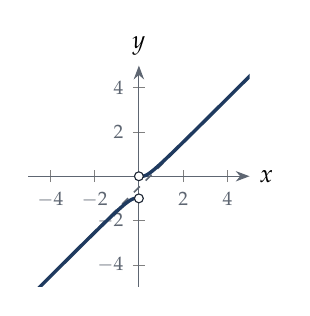
\begin{tikzpicture}
\begin{axis}[courbe,width=0.42\linewidth,xmin=-5,xmax=5,ymin=-5,ymax=5]
\addplot[asy,domain=-5:5,samples=2]{x-0.5};
\addplot[arcetude,domain=0.19:9,samples=300]({1/x},{1/(exp(x)-1)});
\addplot[arcetude,domain=-9:-0.205,samples=300]({1/x},{1/(exp(x)-1)});
\draw[Ink,fill=white] (axis cs:0,-1) circle (1.6pt);
\draw[Ink,fill=white] (axis cs:0,0) circle (1.6pt);
\end{axis}
\end{tikzpicture}
\end{center}
\end{corrige}
\begin{corrige}{rec-hyp}
\textbf{1.} La fonction $x$ est paire et $y$ impaire : symétrie d'axe $(Ox)$, étude sur $[0,+\infty[$. Le vecteur
$f'(t)=(\sh t,\ch t)$ ne s'annule pas puisque $\ch t\geq1$ ; la tangente en $M(0)=(1,0)$ est verticale. Pour $t\geq0$,
$x$ et $y$ croissent vers $+\infty$, $\frac yx=\th t\to1$ et $y-x=-e^{-t}\to0^-$ : la droite $y=x$ est asymptote,
la courbe étant au-dessous ; par symétrie, $y=-x$ est également asymptote.

\textbf{2.} La relation $\ch^2t-\sh^2t=1$ montre que le support est inclus dans l'hyperbole $\mathcal H:x^2-y^2=1$.

\textbf{3.} L'inclusion est stricte : $(-1,0)\in\mathcal H$, alors que $x(t)=\ch t\geq1$. Plus précisément, le support est
$\mathcal H\cap\{x>0\}$. En effet, si $x^2-y^2=1$ et $x>0$, posons $t=\argsh y$ ; alors $\sh t=y$ et
$x=\sqrt{1+y^2}=\ch t$. Le support de $\Gamma$ est la branche droite de l'hyperbole.
\begin{center}
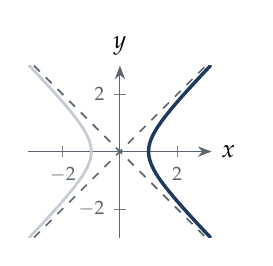
\begin{tikzpicture}
\begin{axis}[courbe,width=0.36\linewidth,xmin=-3.2,xmax=3.2,ymin=-3,ymax=3]
\addplot[asy,domain=-3:3,samples=2]{x};
\addplot[asy,domain=-3:3,samples=2]{-x};
\addplot[Filet,line width=1pt,domain=-1.85:1.85,samples=200]({-cosh(x)},{sinh(x)});
\addplot[arcetude,domain=-1.85:1.85,samples=200]({cosh(x)},{sinh(x)});
\end{axis}
\end{tikzpicture}
\end{center}
\end{corrige}
\begin{corrige}{rec-astro}
Notons $u^{1/3}$ la racine cubique réelle d'un réel $u$. Comme $x=\cos^3t$, on a $x^{1/3}=\cos t$, et de même
$y^{1/3}=\sin t$. Donc $(x^{1/3})^2+(y^{1/3})^2=\cos^2t+\sin^2t=1$, c'est-à-dire $x^{2/3}+y^{2/3}=1$.
\end{corrige}
\begin{corrige}{rec-x4}
L'équation est invariante par $x\mapsto-x$ et par $y\mapsto-y$ : $\mathcal C$ est symétrique par rapport aux deux axes, et
il suffit d'étudier la partie située dans le quart de plan $x\geq0$, $y\geq0$. Comme $(x^2)^2+y^2=1$, on pose
$x^2=\cos\theta$ et $y=\sin\theta$ avec $\theta\in\left[0,\frac\pi2\right]$, soit
\[x(\theta)=\sqrt{\cos\theta},\qquad y(\theta)=\sin\theta.\]
Ce paramétrage décrit exactement l'arc cherché : pour $x,y\geq0$ vérifiant $x^4+y^2=1$, on a $y\in[0,1]$, donc il existe
un unique $\theta\in\left[0,\frac\pi2\right]$ tel que $y=\sin\theta$ ; alors $x^4=1-y^2=\cos^2\theta$, d'où
$x=\sqrt{\cos\theta}$ puisque $x\geq0$.

Sur $\left[0,\frac\pi2\right[$, $x'(\theta)=-\frac{\sin\theta}{2\sqrt{\cos\theta}}\leq0$ et $y'(\theta)=\cos\theta>0$ :
$x$ décroît de $1$ à $0$ et $y$ croît de $0$ à $1$. En $\theta=0$, $f'(0)=(0,1)$ : la tangente en $(1,0)$ est verticale.

En $\theta=\frac\pi2$, la fonction $x$ n'est pas dérivable. On étudie alors $\mathcal C$ au voisinage de $(0,1)$ comme le
graphe de $g(x)=\sqrt{1-x^4}=1-\frac{x^4}2+o(x^4)$ : la tangente en $(0,1)$ est horizontale et la courbe est au-dessous,
avec un contact très plat. Le support complet s'obtient par les deux symétries d'axes.
\begin{center}
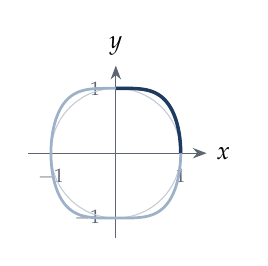
\begin{tikzpicture}
\begin{axis}[courbe,width=0.36\linewidth,xmin=-1.35,xmax=1.4,ymin=-1.3,ymax=1.35,xtick={-1,1},ytick={-1,1}]
\addplot[Filet,domain=0:2*pi,samples=200]({cos(x)},{sin(x)});
\addplot[reste,domain=0:2*pi,samples=400]({sign(cos(x))*sqrt(abs(cos(x)))},{sin(x)});
\addplot[arcetude,domain=0:pi/2,samples=200]({sqrt(abs(cos(x)))},{sin(x)});
\end{axis}
\end{tikzpicture}

{\small\color{Gris}La courbe $x^4+y^2=1$, comparée au cercle unité (trait fin).}
\end{center}
\end{corrige}
\begin{corrige}{b-noeud}
\paragraph{Réduction} $x$ est paire et $y$ impaire : symétrie d'axe $(Ox)$, étude sur $[0,+\infty[$.

\paragraph{Variations} $x'(t)=2t$ et $y'(t)=3t^2-1$ ne s'annulent pas simultanément : la courbe est régulière. En $0$,
$f'(0)=(0,-1)$ : tangente verticale en $O$. Pour $t_1=\frac1{\sqrt3}$, $y'(t_1)=0$ et $x'(t_1)\neq0$ : tangente
horizontale en $M(t_1)=\left(\frac13,-\frac2{3\sqrt3}\right)$, car $y(t_1)=t_1(t_1^2-1)=-\frac2{3\sqrt3}$.
\begin{center}
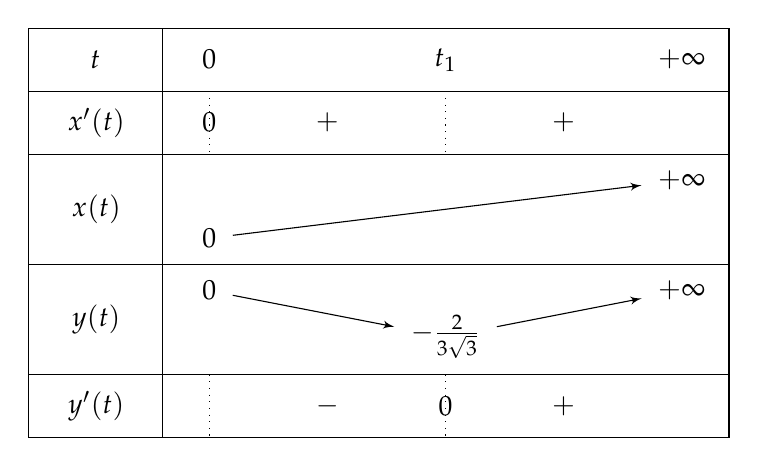
\begin{tikzpicture}
\tkzTabInit[lgt=1.7,espcl=3,deltacl=0.6]{$t$/0.8,$x'(t)$/0.8,$x(t)$/1.4,$y(t)$/1.4,$y'(t)$/0.8}{$0$,$t_1$,$+\infty$}
\tkzTabLine{z,+,t,+,}
\tkzTabVar{-/$0$,R/,+/$+\infty$}
\tkzTabVar{+/$0$,-/$-\frac{2}{3\sqrt3}$,+/$+\infty$}
\tkzTabLine{t,-,z,+,}
\end{tikzpicture}
\end{center}

\paragraph{Branches infinies} Lorsque $t\to\pm\infty$, $\frac yx\sim t\to\pm\infty$ : branches paraboliques de direction
$(Oy)$.

\paragraph{Point double} Comme $x$ est paire, deux paramètres distincts donnant le même point vérifient $s=-t$, avec
$t\neq0$, et alors $y(-t)=y(t)$ impose $y(t)=0$, soit $t^3-t=0$ : $t=\pm1$. Le point $(1,0)$ est atteint pour $t=1$ et
$t=-1$. Les tangentes y sont dirigées par $f'(1)=(2,2)$ et $f'(-1)=(-2,2)$ : ce sont les droites $y=x-1$ et $y=-x+1$,
perpendiculaires.
\begin{center}
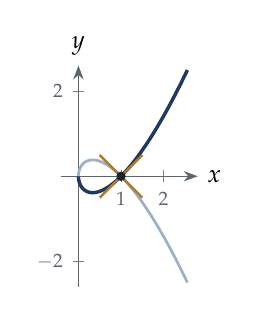
\begin{tikzpicture}
\begin{axis}[courbe,width=0.42\linewidth,xmin=-0.4,xmax=2.8,ymin=-2.6,ymax=2.6]
\addplot[reste,domain=-1.6:0,samples=200]({x^2},{x^3-x});
\addplot[arcetude,domain=0:1.6,samples=200]({x^2},{x^3-x});
\addplot[tgte,domain=0.5:1.5,samples=2]{x-1};
\addplot[tgte,domain=0.5:1.5,samples=2]{-x+1};
\node[pt] at (axis cs:1,0) {};
\end{axis}
\end{tikzpicture}
\end{center}
\end{corrige}
\begin{corrige}{b-astro}
\textbf{1.} $f$ est $2\pi$-périodique. $f(-t)=(\cos^3t,-\sin^3t)$ : symétrie d'axe $(Ox)$, on se ramène à $[0,\pi]$.
$f(\pi-t)=(-\cos^3t,\sin^3t)$ : symétrie d'axe $(Oy)$, et $t\mapsto\pi-t$ échange $[0,\frac\pi2]$ et $[\frac\pi2,\pi]$ :
on se ramène à $[0,\frac\pi2]$. Enfin $f\left(\frac\pi2-t\right)=(\sin^3t,\cos^3t)$ : symétrie d'axe $y=x$, et
$t\mapsto\frac\pi2-t$ échange $[0,\frac\pi4]$ et $[\frac\pi4,\frac\pi2]$. On étudie sur $[0,\frac\pi4]$, puis on complète par
la symétrie d'axe $y=x$, puis d'axe $(Oy)$, puis d'axe $(Ox)$.

\textbf{2.} $f'(t)=(-3\cos^2t\sin t,\ 3\sin^2t\cos t)=3\sin t\cos t\,(-\cos t,\sin t)$. Sur $[0,\frac\pi4]$, le seul point
stationnaire est $M(0)=(1,0)$ ; ailleurs, $x$ décroît et $y$ croît, de $(1,0)$ à
$M\left(\frac\pi4\right)=\left(\frac{\sqrt2}4,\frac{\sqrt2}4\right)$. En $0$,
$\cos^3h=\left(1-\frac{h^2}2\right)^3+o(h^3)=1-\frac32h^2+o(h^3)$ et $\sin^3h=h^3+o(h^3)$ :
$f(h)=(1,0)+h^2\left(-\tfrac32,0\right)+h^3(0,1)+o(h^3)$. Rebroussement de première espèce, tangente horizontale. Par
symétrie, les quatre points $(\pm1,0)$ et $(0,\pm1)$ sont des rebroussements.

\textbf{3.} Pour $t\notin\frac\pi2\Z$, la tangente est dirigée par $(-\cos t,\sin t)$ ; d'après~\eqref{eq:tgte},
\[\sin t\,(x-\cos^3t)+\cos t\,(y-\sin^3t)=0,\]
c'est-à-dire $x\sin t+y\cos t=\sin t\cos t\,(\cos^2t+\sin^2t)=\sin t\cos t$.
Pour $y=0$, $x=\cos t$ ; pour $x=0$, $y=\sin t$. Ainsi $P(\cos t,0)$, $Q(0,\sin t)$ et $PQ=\sqrt{\cos^2t+\sin^2t}=1$ : le
segment de tangente découpé par les axes a une longueur constante.
\begin{center}
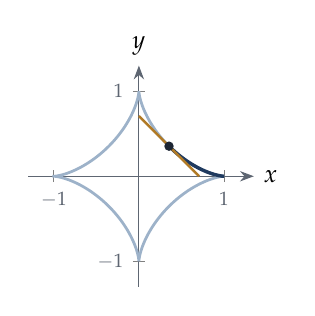
\begin{tikzpicture}
\begin{axis}[courbe,width=0.42\linewidth,xmin=-1.3,xmax=1.35,ymin=-1.3,ymax=1.3,xtick={-1,1},ytick={-1,1}]
\addplot[reste,domain=0:2*pi,samples=400]({cos(x)^3},{sin(x)^3});
\addplot[arcetude,domain=0:pi/4,samples=100]({cos(x)^3},{sin(x)^3});
\draw[tgte] (axis cs:0.7071,0)--(axis cs:0,0.7071);
\node[pt] at (axis cs:0.3536,0.3536) {};
\end{axis}
\end{tikzpicture}

{\small\color{Gris}L'astroïde et le segment $[PQ]$ pour $t=\frac\pi4$.}
\end{center}
\end{corrige}
\begin{corrige}{c-der}
$(te^{-t})'=e^{-t}-te^{-t}=(1-t)e^{-t}$ ; $\big(\ln(1+t^2)\big)'=\frac{2t}{1+t^2}$ ;
$\left(\frac1{\ch t}\right)'=-\frac{\sh t}{\ch^2t}$ ; $(t-\th t)'=1-(1-\th^2t)=\th^2t$.
\end{corrige}
\begin{corrige}{c-sh}
$\ch t_0=\sqrt{1+\sh^2t_0}=\sqrt2$ (car $\ch t_0>0$), $\th t_0=\frac{\sh t_0}{\ch t_0}=\frac1{\sqrt2}$. Enfin
$e^{t_0}=\ch t_0+\sh t_0=1+\sqrt2$, donc $t_0=\ln(1+\sqrt2)$.
\end{corrige}
\begin{corrige}{b-tract}
\textbf{1.} La fonction $x$ est impaire et $y$ paire : le support est symétrique par rapport à $(Oy)$, et l'on étudie sur
$[0,+\infty[$. D'après l'exercice~\ref{e:c-der},
\[x'(t)=\th^2t,\qquad y'(t)=-\frac{\sh t}{\ch^2t},\qquad\text{soit}\qquad f'(t)=\frac{\sh t}{\ch^2t}\,(\sh t,-1),\]
car $\th^2t=\frac{\sh t}{\ch^2t}\cdot\sh t$. Le seul point stationnaire est $M(0)=(0,1)$. Pour $t>0$, $x'>0$ et $y'<0$ :
$x$ croît de $0$ à $+\infty$ et $y$ décroît de $1$ à $0$. Lorsque $t\to+\infty$, $y\to0^+$ : l'axe $(Ox)$ est asymptote
et la courbe est au-dessus.

En $0$, $x(h)=h-\left(h-\frac{h^3}3\right)+o(h^3)=\frac{h^3}3+o(h^3)$ et
$y(h)=\left(1+\frac{h^2}2+o(h^3)\right)^{-1}=1-\frac{h^2}2+o(h^3)$, donc
\[f(h)=(0,1)+h^2\left(0,-\tfrac12\right)+h^3\left(\tfrac13,0\right)+o(h^3).\]
Avec $p=2$ et $q=3$, $M(0)$ est un point de rebroussement de première espèce, à tangente verticale.

\textbf{2.} Pour $t\neq0$, la tangente est dirigée par $(\sh t,-1)$ et a pour pente $-\frac1{\sh t}$ ; elle vaut $-1$ si et
seulement si $\sh t=1$, c'est-à-dire $t=t_0=\ln(1+\sqrt2)$, avec $\ch t_0=\sqrt2$ et $\th t_0=\frac1{\sqrt2}$
(exercice~\ref{e:c-sh}). Le point cherché est
\[A=\left(\ln(1+\sqrt2)-\tfrac{\sqrt2}2,\ \tfrac{\sqrt2}2\right),\]
et la tangente en $A$ a pour équation $y-\frac{\sqrt2}2=-\left(x-\ln(1+\sqrt2)+\frac{\sqrt2}2\right)$, soit
$y=-x+\ln(1+\sqrt2)$.

\textbf{3.} La tangente $T_t=\{M(t)+\lambda(\sh t,-1),\ \lambda\in\R\}$ n'est pas horizontale ; elle coupe donc $(Ox)$
en un unique point, obtenu pour $\frac1{\ch t}-\lambda=0$, c'est-à-dire $\lambda=\frac1{\ch t}$. On trouve
$N=\left(t-\th t+\frac{\sh t}{\ch t},0\right)=(t,0)$ et
\[MN=|\lambda|\,\big\|(\sh t,-1)\big\|=\frac{\sqrt{\sh^2t+1}}{\ch t}=1.\]
Le segment de tangente compris entre la courbe et son asymptote est de longueur constante : c'est la propriété
caractéristique de la tractrice, trajectoire d'un objet tiré par une corde de longueur $1$ dont l'autre extrémité
glisse sur $(Ox)$. On retrouve d'ailleurs que la tangente en $A$ coupe $(Ox)$ au point d'abscisse
$t_0=\ln(1+\sqrt2)$.
\begin{center}
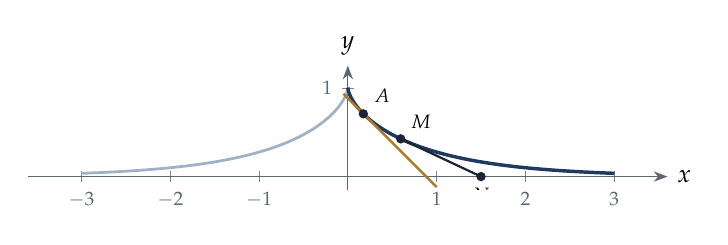
\begin{tikzpicture}
\begin{axis}[courbe,width=0.8\linewidth,xmin=-3.6,xmax=3.6,ymin=-0.15,ymax=1.25,ytick={1}]
\addplot[reste,domain=-4:0,samples=300]({x-tanh(x)},{1/cosh(x)});
\addplot[arcetude,domain=0:4,samples=300]({x-tanh(x)},{1/cosh(x)});
\addplot[tgte,domain=-0.05:1.0,samples=2]{-x+0.8814};
\node[pt] at (axis cs:0.1743,0.7071) {};
\node[font=\scriptsize,anchor=south west] at (axis cs:0.19,0.72) {$A$};
\draw[Ink,line width=0.8pt] (axis cs:0.5949,0.4251)--(axis cs:1.5,0);
\node[pt] at (axis cs:0.5949,0.4251) {}; \node[font=\scriptsize,anchor=south west] at (axis cs:0.6,0.43) {$M$};
\node[pt] at (axis cs:1.5,0) {}; \node[font=\scriptsize,anchor=north] at (axis cs:1.5,-0.02) {$N$};
\end{axis}
\end{tikzpicture}

{\small\color{Gris}La tractrice, la tangente en $A$, et un segment $[MN]$ de longueur $1$ ($t=1{,}5$).}
\end{center}
\end{corrige}
\begin{corrige}{b-folium}
\textbf{1 et 2.} L'origine appartient à $\mathcal C$, et c'est le seul point de $\mathcal C$ d'abscisse nulle (si $x=0$,
l'équation donne $y^3=0$). Un point $M\neq O$ de $\mathcal C$ s'écrit donc $(x,tx)$ avec $x\neq0$, où $t=\frac yx$ est la
pente de la droite $(OM)$. L'équation devient $x^3(1+t^3)=3tx^2$, d'où $t\neq-1$ (sinon $3tx^2=-3x^2=0$) et
\[x(t)=\frac{3t}{1+t^3},\qquad y(t)=\frac{3t^2}{1+t^3},\qquad t\in\R\setminus\{-1\}.\]
Réciproquement, ces points vérifient l'équation. Comme pour le cercle de l'exemple~\ref{ex:cercle-pente}, $M(t)$ est le
second point d'intersection de $\mathcal C$ avec la droite $y=tx$ ; le paramètre $t=0$ redonne $O$.

\textbf{3.} Pour $t\neq0$, $x\left(\frac1t\right)=\frac{3/t}{1+1/t^3}=\frac{3t^2}{t^3+1}=y(t)$ et de même
$y\left(\frac1t\right)=x(t)$ : $M(1/t)$ est le symétrique de $M(t)$ par rapport à la droite $y=x$. Comme $t\mapsto\frac1t$
échange $]-1,0[\,\cup\,]0,1]$ et $]-\infty,-1[\,\cup\,[1,+\infty[$, on étudie la courbe sur $]-1,1]$.

\textbf{4.} \emph{Variations.}
\[x'(t)=\frac{3(1-2t^3)}{(1+t^3)^2},\qquad y'(t)=\frac{3t(2-t^3)}{(1+t^3)^2}.\]
Sur $]-1,1]$, $x'$ s'annule en $t_1=2^{-1/3}$ et $y'$ en $0$ ; il n'y a pas de point stationnaire. La tangente est
horizontale en $M(0)=O$, verticale en $M(t_1)=\left(2^{2/3},2^{1/3}\right)$. En $M(1)=\left(\frac32,\frac32\right)$,
$f'(1)=\frac34(-1,1)$ : la tangente est perpendiculaire à $y=x$, comme l'impose la symétrie.
\begin{center}
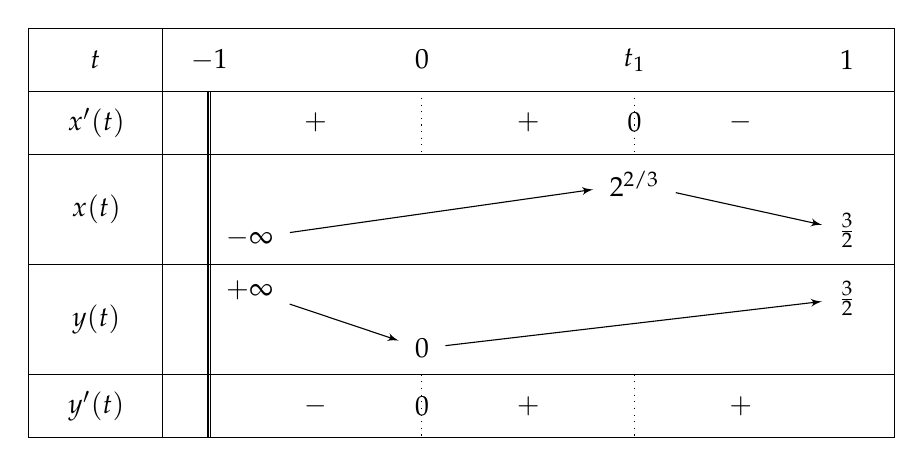
\begin{tikzpicture}
\tkzTabInit[lgt=1.7,espcl=2.7,deltacl=0.6]{$t$/0.8,$x'(t)$/0.8,$x(t)$/1.4,$y(t)$/1.4,$y'(t)$/0.8}{$-1$,$0$,$t_1$,$1$}
\tkzTabLine{d,+,t,+,z,-,}
\tkzTabVar{D-/$-\infty$,R/,+/$2^{2/3}$,-/$\frac32$}
\tkzTabVar{D+/$+\infty$,-/$0$,R/,+/$\frac32$}
\tkzTabLine{d,-,z,+,t,+,}
\end{tikzpicture}
\end{center}

\emph{Branche infinie.} Lorsque $t\to-1^+$, $x\to-\infty$, $y\to+\infty$ et $\frac yx=t\to-1$. De plus,
\[y+x=\frac{3t(1+t)}{1+t^3}=\frac{3t}{1-t+t^2}\xrightarrow[t\to-1]{}-1,\]
car $1+t^3=(1+t)(1-t+t^2)$. La droite $\mathcal A:y=-x-1$ est asymptote. Comme
$y+x+1=\frac{3t+1-t+t^2}{1-t+t^2}=\frac{(t+1)^2}{1-t+t^2}>0$, la courbe est au-dessus de $\mathcal A$, de part et d'autre
par symétrie.

\emph{Point double.} L'origine est atteinte pour $t=0$, et c'est aussi la limite de $M(t)$ lorsque $t\to\pm\infty$ : la
courbe passe deux fois par $O$, avec une tangente horizontale puis, par symétrie, verticale.
\begin{center}
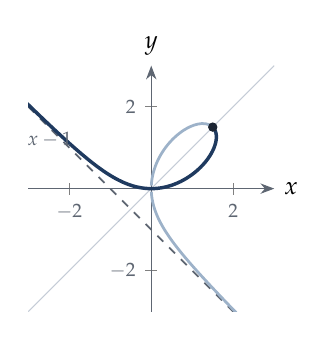
\begin{tikzpicture}
\begin{axis}[courbe,width=0.45\linewidth,xmin=-3,xmax=3,ymin=-3,ymax=3]
\addplot[asy,domain=-3:3,samples=2]{-x-1};
\addplot[Filet,domain=-3:3,samples=2]{x};
\addplot[arcetude,domain=-0.7:1,samples=300]({3*x/(1+x^3)},{3*x^2/(1+x^3)});
\addplot[reste,domain=1:40,samples=400]({3*x/(1+x^3)},{3*x^2/(1+x^3)});
\addplot[reste,domain=-40:-1.43,samples=400]({3*x/(1+x^3)},{3*x^2/(1+x^3)});
\node[Gris,font=\scriptsize,anchor=east] at (axis cs:-1.7,1.15) {$y=-x-1$};
\node[pt] at (axis cs:1.5,1.5) {};
\end{axis}
\end{tikzpicture}

{\small\color{Gris}Le folium de Descartes ; en trait foncé, l'arc $t\in\,]-1,1]$.}
\end{center}
\end{corrige}

\subsection*{Chapitre 6 --- Entraînement TD et DS}
\addcontentsline{toc}{subsection}{Chapitre 6 --- Entraînement TD et DS}
\markboth{7\quad Corrigés --- Chapitre 6}{}
\begin{corrige}{det-choix}
\demarche{on lit la structure avant de calculer : somme constante, variable isolée dans une colonne, colonnes liées, puissances successives.}
$D_1$ : \emph{somme constante} $a+3$ sur chaque ligne. $C_1\leftarrow C_1+C_2+C_3$, on sort $a+3$, puis $L_2\leftarrow L_2-L_1$,
$L_3\leftarrow L_3-L_1$ : $D_1=(a+3)\dt{1&1&1\\0&a&0\\0&0&a}=a^2(a+3)$.

$D_2$ : \emph{déterminant vu comme un polynôme} (méthode~\ref{meth:poly}). Remplaçons $c$ par $x$ : en développant selon la
dernière colonne $(1,x,x^3)$, $P(x)$ est un polynôme de degré $3$, \emph{sans terme en $x^2$}, de coefficient dominant
$\dt{1&1\\a&b}=b-a$. Il s'annule en $a$ et $b$ (deux colonnes égales), donc $P(x)=(b-a)(x-a)(x-b)(x-r)$ ; le coefficient de
$x^2$, $-(b-a)(a+b+r)$, est nul, d'où $r=-(a+b)$ (si $a\neq b$). Ainsi
$D_2=(b-a)(c-a)(c-b)(a+b+c)$, formule qui reste vraie si $a=b$ (les deux membres sont nuls).

$D_3$ : \emph{colonnes liées}. $\cos(i+j)=\cos i\cos j-\sin i\sin j$ : la colonne $j$ vaut $\cos j\,U-\sin j\,V$, avec
$U=(\cos i)_i$ et $V=(\sin i)_i$. Pour $n\geq3$, les colonnes sont dans un espace de dimension au plus $2$ : $D_3=0$. Pour
$n=2$ : $\cos2\cos4-\cos^23=\frac{\cos6+\cos2}2-\frac{1+\cos6}2=\frac{\cos2-1}2=-\sin^21$.

$D_4$ : \emph{Vandermonde}. La ligne $i$ est $(1,i,i^2,\dots,i^{n-1})$ : c'est $V(1,2,\dots,n)=\prod_{1\leq i<j\leq n}(j-i)$.
Pour $j$ fixé, $\prod_{i<j}(j-i)=(j-1)!$, d'où $D_4=1!\,2!\cdots(n-1)!$.
\end{corrige}
\begin{corrige}{det-pb}
\demarche{les coefficients au-dessus et au-dessous de la diagonale sont constants : méthode de la fonction affine (méthode~\ref{meth:affine}), avec les deux valeurs de $c$ qui rendent la matrice triangulaire.}
\textbf{1.} Notons $D(c)$ le déterminant obtenu en ajoutant $c$ à tous les coefficients ; $c\mapsto D(c)$ est affine. Pour
$c=-1$, les coefficients au-dessus de la diagonale s'annulent : matrice triangulaire inférieure de diagonale $x-1$, donc
$D(-1)=(x-1)^n$. Pour $c=1$, ce sont ceux du dessous : $D(1)=(x+1)^n$. Pour une fonction affine,
$D(0)=\frac{D(1)+D(-1)}2$, d'où la formule.

\textbf{2.} Si $n$ est pair, $(x+1)^n$ et $(x-1)^n$ sont positifs et ne s'annulent pas en même temps : $\det M_n(x)>0$, la
matrice est toujours inversible. Si $n$ est impair, $\det M_n(x)=0\iff(x+1)^n=(1-x)^n\iff x+1=1-x$ (la fonction
$u\mapsto u^n$ est injective) $\iff x=0$ : $M_n(x)$ est inversible si et seulement si $x\neq0$.

\textbf{3.} $M_n(0)$ est antisymétrique. Pour $n$ impair, son déterminant est nul, comme le prévoit l'exercice~\ref{e:g-antisym} ;
pour $n$ pair, il vaut $\frac{1+1}2=1$.

\textbf{4.} Pour $n=3$ : $\det M_3(x)=\frac{(x+1)^3+(x-1)^3}2=x^3+3x=x(x^2+3)$, nul seulement en $0$ ; d'où la caractérisation
des bases. Sarrus : $\dt{x&1&1\\-1&x&1\\-1&-1&x}=(x^3-1+1)-(-x-x-x)=x^3+3x$.
\end{corrige}
\begin{corrige}{td-tab}
\demarche{chaque colonne du tableau donne un point et, par $(x',y')$, la direction de la tangente ; chaque intervalle donne une direction de déplacement (réflexe de l'étape 13).}
\textbf{1.} Points et tangentes : $M(0)=(1,0)$ et $M(\pi)=(-1,0)$ avec $f'=(0,2)$, tangentes verticales ;
$M\left(\frac\pi4\right)=\left(\frac{\sqrt2}2,1\right)$ et $M\left(\frac{3\pi}4\right)=\left(-\frac{\sqrt2}2,-1\right)$, tangentes horizontales ;
$M\left(\frac\pi2\right)=O$ avec $f'=(-1,-2)$. Sur $\left[0,\frac\pi4\right]$, $(x',y')$ a les signes $(-,+)$ : vers le haut
à gauche ; puis $(-,-)$ jusqu'à $\frac{3\pi}4$ : vers le bas à gauche, en traversant $O$ ; puis $(-,+)$ : vers le haut à
gauche jusqu'à $(-1,0)$. L'arc a la forme d'un « S » couché (trait plein ci-dessous).

\textbf{2.} En $O$, $f'\left(\frac\pi2\right)=(-1,-2)$ : $\det\big((x,y),(-1,-2)\big)=-2x+y=0$, soit $y=2x$.

\textbf{3.} $x'<0$ sur $]0,\pi[$ : $x$ est strictement décroissante, donc injective, et $f$ aussi (deux paramètres
distincts donnent deux abscisses distinctes). L'arc $\Gamma_0$ n'a pas de point double.

\textbf{4.} (a) $M(-t)=(x(t),-y(t))$ : on complète $\Gamma_0$ par son symétrique par rapport à $(Ox)$. On obtient une courbe en
forme de « huit ». Le point $O=M\left(\frac\pi2\right)$ a pour symétrique $M\left(-\frac\pi2\right)=O$ : c'est un point
double, de tangentes $y=2x$ et $y=-2x$ (la tangente symétrique). Les points $(\pm1,0)$, sur l'axe et à tangente
perpendiculaire à l'axe, sont des points de raccord, non des points doubles.

(b) $M(-t)=M(t)$ : la courbe sur $[-\pi,0]$ est $\Gamma_0$ parcourue en sens inverse ; le support reste $\Gamma_0$.

(c) Si $f$ était impaire, on aurait $f(0)=-f(0)$, donc $M(0)=O$ ; or $M(0)=(1,0)$ : impossible. Si $f$ était
$\pi$-périodique, on aurait $M(\pi)=M(0)$ ; or $(-1,0)\neq(1,0)$ : impossible. Avant d'utiliser une hypothèse de symétrie,
on vérifie sa compatibilité avec le tableau.

\textbf{5.} $x'=-\sin t$ et $y'=2\cos2t$ donnent bien les valeurs de la première et de la dernière ligne, et $x$, $y$
prennent les valeurs indiquées ($\sin\frac\pi2=1$, $\sin\frac{3\pi}2=-1$\dots). Pour cette fonction, $x$ est paire et $y$
impaire : c'est le cas (a) qui est réalisé.
\begin{center}
\begin{tikzpicture}
\begin{axis}[courbe,width=0.5\linewidth,xmin=-1.3,xmax=1.3,ymin=-1.25,ymax=1.25,xtick={-1,1},ytick={-1,1}]
\addplot[reste,domain=-3.1416:0,samples=200]({cos(x)},{sin(2*x)});
\addplot[arcetude,domain=0:3.1416,samples=200]({cos(x)},{sin(2*x)});
\addplot[tgte,domain=-0.35:0.35,samples=2]{2*x};
\addplot[tgte,domain=-0.35:0.35,samples=2]{-2*x};
\node[pt] at (axis cs:0,0) {};
\end{axis}
\end{tikzpicture}
\end{center}
\end{corrige}
\begin{corrige}{echelle}
\demarche{lieu géométrique : on choisit le paramètre naturel (l'angle), on exprime les points, puis on traduit « tangente » par une colinéarité, donc un déterminant nul.}
\textbf{1.} $P=(L\cos\theta,0)$ et $Q=(0,L\sin\theta)$. Comme $QM=a$ sur un segment de longueur $L$,
$M=Q+\frac aL\vv{QP}=(0,L\sin\theta)+\frac aL(L\cos\theta,-L\sin\theta)=(a\cos\theta,(L-a)\sin\theta)=(a\cos\theta,b\sin\theta)$.
Le point $M$ décrit le quart d'ellipse $\frac{x^2}{a^2}+\frac{y^2}{b^2}=1$, $x,y\geq0$. Si $a=b$, c'est un quart de cercle
de rayon $a$ : le milieu de l'échelle reste à distance $\frac L2$ du coin $O$.

\textbf{2.} La trajectoire est dirigée par $M'(\theta)=(-a\sin\theta,b\cos\theta)\neq\ve0$ et l'échelle par
$\vv{QP}/L=(\cos\theta,-\sin\theta)$. L'échelle passe toujours par $M$ ; elle est tangente à la trajectoire en $M$ si et
seulement si ces vecteurs sont colinéaires :
\[\dt{-a\sin\theta&\cos\theta\\b\cos\theta&-\sin\theta}=a\sin^2\theta-b\cos^2\theta=0\iff\tan\theta=\sqrt{\tfrac ba}.\]
Pour $a=2$, $b=1$ : $\tan\theta=\frac1{\sqrt2}$, $\theta\approx35{,}3^\circ$.

\textbf{3.} La droite $(PQ)$ a pour équation $\frac x{L\cos\theta}+\frac y{L\sin\theta}=1$, et
$\frac{L\cos^3\theta}{L\cos\theta}+\frac{L\sin^3\theta}{L\sin\theta}=\cos^2\theta+\sin^2\theta=1$ : $A(\theta)$ est sur
l'échelle. Puis $A'(\theta)=3L\sin\theta\cos\theta\,(-\cos\theta,\sin\theta)$, non nul et colinéaire à
$(\cos\theta,-\sin\theta)$ pour $\theta\in\left]0,\frac\pi2\right[$ : l'échelle est tangente en $A(\theta)$ à la courbe
décrite par $A$, un quart d'\emph{astroïde}. Chaque position de l'échelle est tangente à cette courbe : on dit que
l'astroïde est l'\emph{enveloppe} des positions de l'échelle.
\begin{center}
\begin{tikzpicture}
\begin{axis}[courbe,width=0.5\linewidth,xmin=-0.2,xmax=3.3,ymin=-0.2,ymax=3.3,xtick={1,2,3},ytick={1,2,3}]
\addplot[Gris,thin] coordinates {(2.819,0) (0,1.026)};
\addplot[Gris,thin] coordinates {(1.721,0) (0,2.457)};
\addplot[Gris,thin] coordinates {(0.776,0) (0,2.898)};
\addplot[Ocre,thick] coordinates {(2.449,0) (0,1.732)};
\addplot[arcetude,domain=0:1.5708,samples=100]({2*cos(x)},{sin(x)});
\addplot[Brique,thick,domain=0:1.5708,samples=100]({3*cos(x)^3},{3*sin(x)^3});
\node[pt] at (axis cs:1.633,0.577) {};
\node[font=\scriptsize,anchor=south west] at (axis cs:1.65,0.6) {$M$};
\end{axis}
\end{tikzpicture}
\end{center}
En bleu le quart d'ellipse décrit par $M$ ($a=2$, $b=1$), en brique l'astroïde ; en gris trois positions de l'échelle, en
ocre la position où elle est tangente à l'ellipse en $M$.
\end{corrige}
\begin{corrige}{loc-e}
\demarche{méthode~\ref{meth:dl} : développement à l'ordre 3, car le premier vecteur est en $t^2$ et l'on attend le second en $t^3$ ; on vérifie la non-colinéarité avant de conclure.}
$x'(t)=1-\frac1{1+t}$ et $y'(t)=\sqrt{1+t}-1+\frac t{2\sqrt{1+t}}$ s'annulent en $0$. Avec
$\ln(1+t)=t-\frac{t^2}2+\frac{t^3}3+o(t^3)$ et $\sqrt{1+t}=1+\frac t2-\frac{t^2}8+o(t^2)$ :
\[x(t)=\frac{t^2}2-\frac{t^3}3+o(t^3),\qquad y(t)=\frac{t^2}2-\frac{t^3}8+o(t^3),\]
\[f(t)=t^2\left(\tfrac12,\tfrac12\right)+t^3\left(-\tfrac13,-\tfrac18\right)+o(t^3).\]
$\det\big((\frac12,\frac12),(-\frac13,-\frac18)\big)=-\frac1{16}+\frac16=\frac5{48}\neq0$ : $p=2$, $q=3$, rebroussement de
première espèce en $O$, de tangente $y=x$. Le vecteur $\ve b=\left(-\frac13,-\frac18\right)$ vérifie $y-x=\frac5{24}>0$ : pour
$t>0$, la courbe est au-dessus de $y=x$, pour $t<0$ au-dessous ; les deux arcs partent de $O$ dans la direction de
$\ve a=\left(\frac12,\frac12\right)$. Le cours traite de la même façon $\big(t-2\sqrt{1+t},\ t\ln(1-t)\big)$ en $0$.
\begin{center}
\begin{tikzpicture}
\begin{axis}[courbe,width=0.36\linewidth,xmin=-0.02,xmax=0.42,ymin=-0.02,ymax=0.42,xtick=\empty,ytick=\empty]
\addplot[asy,domain=0:0.4,samples=2]{x};
\addplot[arcetude,domain=-0.6:0.75,samples=200]({x-ln(1+x)},{x*(sqrt(1+x)-1)});
\node[pt] at (axis cs:0,0) {};
\end{axis}
\end{tikzpicture}
\end{center}
\end{corrige}
\begin{corrige}{infl2}
\demarche{méthode~\ref{meth:inflexion} : candidats par $\det(f',f'')=0$, confirmation par le changement de signe ; la pente se dérive avec l'astuce qui suit la méthode.}
\textbf{1.} $x'(t)=3(t+1)^2\geq0$ et $y'(t)=2t$ ne s'annulent jamais ensemble : courbe régulière. En $t=-1$, $f'=(0,-2)$ :
tangente verticale en $M(-1)=O$ ; en $t=0$, $f'=(3,0)$ : tangente horizontale en $M(0)=(1,-1)$.
\begin{center}
\begin{tikzpicture}
\tkzTabInit[lgt=1.7,espcl=2.2,deltacl=0.6]{$t$/0.8,$x'(t)$/0.8,$x(t)$/1.4,$y(t)$/1.4,$y'(t)$/0.8}{$-\infty$,$-1$,$0$,$1$,$+\infty$}
\tkzTabLine{,+,z,+,t,+,t,+,}
\tkzTabVar{-/$-\infty$,R/,R/,R/,+/$+\infty$}
\tkzTabIma{1}{5}{2}{$0$}
\tkzTabIma{1}{5}{3}{$1$}
\tkzTabIma{1}{5}{4}{$8$}
\tkzTabVar{+/$+\infty$,R/,-/$-1$,R/,+/$+\infty$}
\tkzTabIma{1}{3}{2}{$0$}
\tkzTabIma{3}{5}{4}{$0$}
\tkzTabLine{,-,t,-,z,+,t,+,}
\end{tikzpicture}
\end{center}
Lorsque $t\to\pm\infty$, $|x|$ et $y$ tendent vers $+\infty$ et $\frac yx\sim\frac1t\to0$ : deux branches paraboliques de
direction $(Ox)$, et aucune asymptote.

\textbf{2.} $f''(t)=\big(6(t+1),2\big)$ et
\[\det\big(f'(t),f''(t)\big)=6(t+1)^2-12t(t+1)=6(t+1)(1-t).\]
Les candidats sont $t=-1$ et $t=1$ ; le déterminant change de signe en chacun (racines simples) : ce sont deux points
d'inflexion, $O$ et $M(1)=(8,0)$. En $O$, la tangente est verticale, $x=0$ : la courbe traverse l'axe $(Oy)$ en
s'appuyant sur lui. En $M(1)$, $f'(1)=(12,2)$, tangente $y=\frac{x-8}6$.

\textbf{3.} $p(t)=\frac{y'(t)}{x'(t)}=\frac{2t}{3(t+1)^2}$ et $p'(t)=\frac{\det(f',f'')}{x'^2}=\frac{2(1-t)}{3(t+1)^3}$. Sur
$]-1,+\infty[$, $p$ croît jusqu'en $t=1$ puis décroît : la pente maximale, $\frac16$, est atteinte au point d'inflexion
$(8,0)$. En $t=-1$, l'autre inflexion, la tangente est verticale : $p$ n'est pas défini et tend vers $-\infty$. L'astuce
« pente extrémale » ne vaut qu'aux inflexions à tangente non verticale.

\textbf{4.}
\begin{center}
\begin{tikzpicture}
\begin{axis}[courbe,width=0.75\linewidth,xmin=-3,xmax=12,ymin=-1.5,ymax=4.5,axis equal image=false,height=0.38\linewidth,xtick={1,8},ytick={-1,1,2,3,4}]
\addplot[arcetude,domain=-2.3:1.3,samples=200]({(x+1)^3},{x^2-1});
\addplot[tgte,samples=2] coordinates {(0,-1.2) (0,1.2)};
\addplot[tgte,domain=5:11,samples=2]{(x-8)/6};
\node[pt,fill=Ocre] at (axis cs:0,0) {}; \node[pt,fill=Ocre] at (axis cs:8,0) {};
\node[pt] at (axis cs:1,-1) {};
\end{axis}
\end{tikzpicture}
\end{center}
\end{corrige}
\begin{corrige}{cardio2}
\demarche{les dérivées sont des sommes de sinus ou de cosinus : on les factorise par l'angle moitié (astuce de la boîte à outils), comme dans le TD pour $\cos t-\cos2t$.}
\textbf{1.} $x$ est paire, $y$ impaire, $f$ est $2\pi$-périodique : symétrie d'axe $(Ox)$, étude sur $[0,\pi]$.

\textbf{2.} $x=\cos t+\cos^2t$ et $y=\sin t+\frac12\sin2t$, d'où $x'=-(\sin t+\sin2t)$ et $y'=\cos t+\cos2t$. Or
$e^{it}+e^{2it}=e^{\frac{3it}2}\left(e^{-\frac{it}2}+e^{\frac{it}2}\right)=2\cos\frac t2\,e^{\frac{3it}2}$ ; en prenant les
parties réelle et imaginaire, $\cos t+\cos2t=2\cos\frac t2\cos\frac{3t}2$ et $\sin t+\sin2t=2\cos\frac t2\sin\frac{3t}2$.

\textbf{3.} Sur $[0,\pi]$, $\cos\frac t2\geq0$, nul seulement en $\pi$. $x'<0$ sur $\left]0,\frac{2\pi}3\right[$ et $x'>0$ sur
$\left]\frac{2\pi}3,\pi\right[$ ; $y'>0$ sur $\left[0,\frac\pi3\right[$ et $y'<0$ sur $\left]\frac\pi3,\pi\right[$.
\begin{center}
\begin{tikzpicture}
\tkzTabInit[lgt=1.7,espcl=2.4,deltacl=0.6]{$t$/0.8,$x'(t)$/0.8,$x(t)$/1.4,$y(t)$/1.4,$y'(t)$/0.8}{$0$,$\frac\pi3$,$\frac{2\pi}3$,$\pi$}
\tkzTabLine{z,-,t,-,z,+,z}
\tkzTabVar{+/$2$,R/,-/$-\frac14$,+/$0$}
\tkzTabIma{1}{3}{2}{$\frac34$}
\tkzTabVar{-/$0$,+/$\frac{3\sqrt3}4$,R/,-/$0$}
\tkzTabIma{2}{4}{3}{$\frac{\sqrt3}4$}
\tkzTabLine{t,+,z,-,t,-,z}
\end{tikzpicture}
\end{center}
Tangente verticale en $M(0)=(2,0)$ et en $M\left(\frac{2\pi}3\right)=\left(-\frac14,\frac{\sqrt3}4\right)$, horizontale en
$M\left(\frac\pi3\right)=\left(\frac34,\frac{3\sqrt3}4\right)$.

\textbf{4.} $f'(\pi)=\ve0$. En $t=\pi+h$ : $1+\cos t=1-\cos h=\frac{h^2}2+o(h^3)$, $\cos t=-\cos h$, $\sin t=-\sin h$, d'où
\[f(\pi+h)=h^2\left(-\tfrac12,0\right)+h^3\left(0,-\tfrac12\right)+o(h^3) :\]
rebroussement de première espèce en $O$, de tangente $(Ox)$ ; la courbe arrive par la gauche ($x\approx-\frac{h^2}2<0$).

\textbf{5.} $\vv{OM(t)}=(1+\cos t)(\cos t,\sin t)$ : en polaire, $r=1+\cos\theta$ (\HP). C'est la cardioïde, déjà
rencontrée dans le cours sous la forme $r=1-\cos\theta$ (la même courbe retournée).
\begin{center}
\begin{tikzpicture}
\begin{axis}[courbe,width=0.48\linewidth,xmin=-0.6,xmax=2.3,ymin=-1.5,ymax=1.5,xtick={1,2},ytick={-1,1}]
\addplot[reste,domain=-3.1416:0,samples=200]({(1+cos(x))*cos(x)},{(1+cos(x))*sin(x)});
\addplot[arcetude,domain=0:3.1416,samples=200]({(1+cos(x))*cos(x)},{(1+cos(x))*sin(x)});
\node[pt] at (axis cs:0,0) {};
\end{axis}
\end{tikzpicture}
\end{center}
\end{corrige}
\begin{corrige}{strophoide}
\demarche{même plan que pour la cissoïde du TD : symétrie, variations, points doubles, asymptote, équation cartésienne.}
\textbf{1.} $x$ est paire, $y$ impaire : $M(-t)$ est le symétrique de $M(t)$ par rapport à $(Ox)$. On étudie sur $[0,+\infty[$.

\textbf{2.} $x'(t)=\dfrac{4t}{(t^2+1)^2}$ et, comme $y=tx$, $y'=x+tx'=\dfrac{(t^2-1)(t^2+1)+4t^2}{(t^2+1)^2}=\dfrac{t^4+4t^2-1}{(t^2+1)^2}$.
$x'$ ne s'annule qu'en $0$, où $y'(0)=-1$ : pas de point stationnaire. $y'$ s'annule pour $t^2=\sqrt5-2$, soit
$t_0=\sqrt{\sqrt5-2}\approx0{,}49$ ; alors $x(t_0)=\frac{\sqrt5-3}{\sqrt5-1}=\frac{1-\sqrt5}2\approx-0{,}62$ et
$y(t_0)=t_0x(t_0)\approx-0{,}30$.
\begin{center}
\begin{tikzpicture}
\tkzTabInit[lgt=1.7,espcl=2.4,deltacl=0.6]{$t$/0.8,$x'(t)$/0.8,$x(t)$/1.4,$y(t)$/1.4,$y'(t)$/0.8}{$0$,$t_0$,$1$,$+\infty$}
\tkzTabLine{z,+,t,+,t,+,}
\tkzTabVar{-/$-1$,R/,R/,+/$1$}
\tkzTabIma{1}{4}{2}{$\frac{1-\sqrt5}2$}
\tkzTabIma{1}{4}{3}{$0$}
\tkzTabVar{+/$0$,-/$\approx-0{,}30$,R/,+/$+\infty$}
\tkzTabIma{2}{4}{3}{$0$}
\tkzTabLine{,-,z,+,t,+,}
\end{tikzpicture}
\end{center}
Tangente verticale en $M(0)=(-1,0)$ (point de l'axe, tangente perpendiculaire à l'axe), horizontale en $M(\pm t_0)$.

\textbf{3.} $x(t)=0\iff t=\pm1$, et alors $y=0$ : $M(1)=M(-1)=O$. $f'(1)=(1,1)$ et $f'(-1)=(-1,1)$ : les tangentes en $O$ sont
$y=x$ et $y=-x$, perpendiculaires.

\textbf{4.} Lorsque $t\to\pm\infty$, $x\to1$ et $y\sim t\to\pm\infty$ : asymptote verticale $x=1$. Comme
$x-1=-\frac2{t^2+1}<0$, la courbe est à gauche de l'asymptote.

\textbf{5.} Pour $x\neq0$, $t=\frac yx$ : c'est la \emph{pente} de la droite $(OM)$. De $x(t^2+1)=t^2-1$ on tire
$t^2=\frac{1+x}{1-x}$, d'où $y^2=t^2x^2=x^2\frac{1+x}{1-x}$, soit $y^2(1-x)=x^2(1+x)$ ; l'égalité vaut aussi en $O$.

\textbf{6.} La boucle correspond à $t\in[-1,1]$, les deux branches infinies à $|t|>1$.
\begin{center}
\begin{tikzpicture}
\begin{axis}[courbe,width=0.42\linewidth,xmin=-1.3,xmax=1.4,ymin=-3,ymax=3,axis equal image=false,height=0.5\linewidth,xtick={-1,1},ytick={-2,2}]
\addplot[asy,samples=2] coordinates {(1,-3) (1,3)};
\addplot[reste,domain=-3.6:0,samples=200]({(x^2-1)/(x^2+1)},{x*(x^2-1)/(x^2+1)});
\addplot[arcetude,domain=0:3.6,samples=200]({(x^2-1)/(x^2+1)},{x*(x^2-1)/(x^2+1)});
\addplot[tgte,domain=-0.35:0.35,samples=2]{x}; \addplot[tgte,domain=-0.35:0.35,samples=2]{-x};
\node[pt] at (axis cs:0,0) {};
\end{axis}
\end{tikzpicture}
\end{center}
\end{corrige}
\begin{corrige}{lemni}
\demarche{fonctions $2\pi$-périodiques : on cherche les transformations $t\mapsto-t$ et $t\mapsto\pi-t$, comme pour la courbe de Lissajous du cours.}
\textbf{1.} $f$ est $2\pi$-périodique. $f(-t)=-f(t)$ : symétrie de centre $O$. $f(\pi-t)=\big(x(t),-y(t)\big)$ : symétrie
d'axe $(Ox)$. On étudie sur $\left[0,\frac\pi2\right]$ ; la symétrie d'axe $(Ox)$ donne $\left[\frac\pi2,\pi\right]$, puis la
symétrie de centre $O$ donne $[-\pi,0]$. La composée des deux est la symétrie d'axe $(Oy)$.

\textbf{2.} Après calcul,
\[x'(t)=\frac{\cos t\,(2+\sin^2t)}{(1+\cos^2t)^2},\qquad y'(t)=\frac{2-3\sin^2t}{(1+\cos^2t)^2}.\]
Sur $\left[0,\frac\pi2\right]$, $x'\geq0$ (nul seulement en $\frac\pi2$) et $y'$ s'annule en $t_1=\arcsin\sqrt{\frac23}$,
positif avant, négatif après. Points : $M(0)=O$, $f'(0)=\left(\frac12,\frac12\right)$, tangente $y=x$ ;
$M(t_1)=\left(\frac{\sqrt6}4,\frac{\sqrt2}4\right)\approx(0{,}61\,;0{,}35)$, tangente horizontale ;
$M\left(\frac\pi2\right)=(1,0)$, $f'=(0,-1)$, tangente verticale.

\textbf{3.} $M(0)=M(\pi)=O$ et $f'(\pi)=\left(-\frac12,\frac12\right)$ : les tangentes en $O$ sont $y=x$ et $y=-x$.

\textbf{4.} $x^2+y^2=\frac{\sin^2t\,(1+\cos^2t)}{(1+\cos^2t)^2}=\frac{\sin^2t}{1+\cos^2t}$ et
$x^2-y^2=\frac{\sin^2t\,(1-\cos^2t)}{(1+\cos^2t)^2}=\frac{\sin^4t}{(1+\cos^2t)^2}=(x^2+y^2)^2$. En polaire
($x=r\cos\theta$, $y=r\sin\theta$) : $r^4=r^2(\cos^2\theta-\sin^2\theta)$, soit $r^2=\cos2\theta$ (pour $r\neq0$) : c'est la
lemniscate de Bernoulli. La lemniscate du TD, $r^2=\frac12\sin2\theta$, est la même courbe tournée de $\frac\pi4$ et
réduite d'un facteur $\frac1{\sqrt2}$ ; son axe de symétrie $y=x$ correspond ici à l'axe $(Ox)$.

\textbf{5.}
\begin{center}
\begin{tikzpicture}
\begin{axis}[courbe,width=0.55\linewidth,xmin=-1.2,xmax=1.2,ymin=-0.55,ymax=0.55,xtick={-1,1},ytick=\empty]
\addplot[reste,domain=0:6.2832,samples=300]({sin(x)/(1+cos(x)^2)},{sin(x)*cos(x)/(1+cos(x)^2)});
\addplot[arcetude,domain=0:1.5708,samples=100]({sin(x)/(1+cos(x)^2)},{sin(x)*cos(x)/(1+cos(x)^2)});
\addplot[tgte,domain=-0.3:0.3,samples=2]{x}; \addplot[tgte,domain=-0.3:0.3,samples=2]{-x};
\node[pt] at (axis cs:0,0) {};
\end{axis}
\end{tikzpicture}
\end{center}
\end{corrige}
\begin{corrige}{bicorne2}
\demarche{point stationnaire : développement limité ; le piège est de s'arrêter trop tôt, car le terme en $t^3$ est nul et celui en $t^4$ peut encore être colinéaire au premier.}
\textbf{1.} $x(\pi-t)=1+\cos t=2-x(t)$ et $y(\pi-t)=y(t)$ : $M(\pi-t)$ est le symétrique de $M(t)$ par rapport à la droite
$x=1$. Avec la $2\pi$-périodicité, on étudie sur $\left[-\frac\pi2,\frac\pi2\right]$, dont l'image par $t\mapsto\pi-t$ est
$\left[\frac\pi2,\frac{3\pi}2\right]$.

\textbf{2.} $f'(t)=\big(\sin t,\ \sin t\cos t\,(2+5\sin^3t)\big)$ s'annule en $0$. À l'ordre $5$ :
$1-\cos t=\frac{t^2}2-\frac{t^4}{24}+o(t^5)$, $\sin^2t=t^2-\frac{t^4}3+o(t^5)$, $\sin^5t=t^5+o(t^5)$, d'où
\[f(t)=t^2\left(\tfrac12,1\right)+t^4\left(-\tfrac1{24},-\tfrac13\right)+t^5(0,1)+o(t^5).\]
Il n'y a pas de terme en $t^3$ ; le vecteur $\ve b=\left(-\frac1{24},-\frac13\right)$ n'est pas colinéaire à
$\ve a=\left(\frac12,1\right)$ ($\det(\ve a,\ve b)=-\frac16+\frac1{24}=-\frac18\neq0$). Donc $p=2$, $q=4$ : rebroussement de
seconde espèce, de tangente $y=2x$. Les deux arcs sont du côté de $\ve b$ (car $t^4>0$), c'est-à-dire sous la droite
$y=2x$ ($\ve b$ vérifie $y-2x=-\frac14<0$). Comme le note le cours, il faut ici aller jusqu'au troisième vecteur non nul
pour voir la différence avec un rebroussement de première espèce.

\textbf{3.} Sur $\left[-\frac\pi2,\frac\pi2\right]$, $\cos t\geq0$ ; $2+5\sin^3t=0$ pour $\sin t=-(2/5)^{1/3}$, soit
$t=\beta\approx-0{,}83$. Signes : sur $\left[-\frac\pi2,\beta\right[$, $x'<0$, $y'>0$ ; sur $]\beta,0[$, $x'<0$, $y'<0$ ; sur
$\left]0,\frac\pi2\right]$, $x'>0$, $y'>0$. Points : $M\left(-\frac\pi2\right)=(1,0)$ et $M\left(\frac\pi2\right)=(1,2)$, tangentes
horizontales (points de l'axe $x=1$) ; $M(\beta)\approx(0{,}32\,;0{,}33)$, tangente horizontale ; $M(0)=O$.

\textbf{4.}
\begin{center}
\begin{tikzpicture}
\begin{axis}[courbe,width=0.5\linewidth,xmin=-0.2,xmax=2.2,ymin=-0.2,ymax=2.2,xtick={1,2},ytick={1,2}]
\addplot[asy,samples=2] coordinates {(1,-0.2) (1,2.2)};
\addplot[reste,domain=1.5708:4.7124,samples=300]({1-cos(x)},{sin(x)^2+sin(x)^5});
\addplot[arcetude,domain=-1.5708:1.5708,samples=300]({1-cos(x)},{sin(x)^2+sin(x)^5});
\addplot[tgte,domain=0:0.35,samples=2]{2*x};
\node[pt] at (axis cs:0,0) {}; \node[pt] at (axis cs:2,0) {};
\end{axis}
\end{tikzpicture}
\end{center}
\end{corrige}
\begin{corrige}{cub-asy}
\demarche{les coordonnées s'échangent quand on remplace $t$ par $1/t$ : symétrie par rapport à $y=x$ ; la branche parabolique se précise par une courbe asymptote (encadré hors programme de la boîte à outils).}
\textbf{1.} $x(1/t)=\frac1t+\frac{t^3}3=y(t)$ et $y(1/t)=x(t)$ : $M(1/t)$ est le symétrique de $M(t)$ par rapport à la
droite $y=x$. $f(-t)=-f(t)$ : symétrie de centre $O$. On étudie sur $[1,+\infty[$ ; la première symétrie donne $]0,1]$, la
seconde $\R_-^*$.

\textbf{2.} $x'(t)=1-\frac1{t^4}=\frac{t^4-1}{t^4}$, $y'(t)=t^2-\frac1{t^2}=\frac{t^4-1}{t^2}$ : points stationnaires en
$t=\pm1$, $M(\pm1)=\pm\left(\frac43,\frac43\right)$. En $t=1+h$ :
\[f(1+h)=\left(\tfrac43,\tfrac43\right)+h^2(2,2)+h^3\left(-\tfrac{10}3,-\tfrac23\right)+o(h^3),\]
avec $\det\big((2,2),(-\frac{10}3,-\frac23)\big)=\frac{16}3\neq0$ : rebroussement de première espèce, de tangente la droite
$y=x$, axe de symétrie (ce qui était prévisible : la tangente en un point stationnaire de l'axe est l'axe lui-même ou sa
perpendiculaire).

\textbf{3.} Sur $[1,+\infty[$, $x$ et $y$ croissent de $\frac43$ à $+\infty$, et $\frac yx\sim\frac{t^2}3\to+\infty$ :
branche parabolique de direction $(Oy)$. Pour la préciser, on compare $y$ à $\frac{x^3}3$ :
$x^3=t^3+3t^2\cdot\frac1{3t^3}+O\!\left(\frac1{t^5}\right)=t^3+\frac1t+O\!\left(\frac1{t^5}\right)$, donc
\[y-\frac{x^3}3=\frac1t-\frac1{3t}+O\!\left(\frac1{t^5}\right)=\frac2{3t}+O\!\left(\frac1{t^5}\right)\xrightarrow[t\to+\infty]{}0^+.\]
Le point $P_t=\big(x(t),\frac{x(t)^3}3\big)$ de $\Gamma$ vérifie $M(t)P_t\to0$ : $\Gamma$ est asymptote, et la courbe est
au-dessus. Par la symétrie d'axe $y=x$, lorsque $t\to0^+$ la courbe est asymptote à la cubique $x=\frac{y^3}3$, à sa droite.

\textbf{4.}
\begin{center}
\begin{tikzpicture}
\begin{axis}[courbe,width=0.55\linewidth,xmin=-4.5,xmax=4.5,ymin=-4.5,ymax=4.5,xtick={-2,2},ytick={-2,2}]
\addplot[asy,domain=-2.4:2.4,samples=60]{x^3/3};
\addplot[asy,domain=-2.4:2.4,samples=60]({x^3/3},{x});
\addplot[Gris,dotted,domain=-4.5:4.5,samples=2]{x};
\addplot[arcetude,domain=0.44:2.35,samples=200]({x+1/(3*x^3)},{x^3/3+1/x});
\addplot[arcetude,domain=-2.35:-0.44,samples=200]({x+1/(3*x^3)},{x^3/3+1/x});
\node[pt] at (axis cs:1.333,1.333) {}; \node[pt] at (axis cs:-1.333,-1.333) {};
\end{axis}
\end{tikzpicture}
\end{center}
\end{corrige}
\begin{corrige}{ds-pb}
\demarche{le problème suit le plan du devoir de la classe : chaque question réinvestit une méthode du livre (factorisation des dérivées, développement en $t_0\neq0$, position globale, asymptotes, courbe asymptote, inflexion par factorisation de la vitesse). On note les valeurs interdites dès le début : $-3$ (borne) et $0$.}

\textbf{1.(a)} $x'(t)=-\frac4{t^2}+\frac1{t+3}=\frac{t^2-4t-12}{t^2(t+3)}=\frac{(t-6)(t+2)}{t^2(t+3)}$ et
$y'(t)=1-\frac4{t^2}=\frac{(t-2)(t+2)}{t^2}$. Comme $t^2>0$ et $t+3>0$, les signes se lisent sur les facteurs affines. Limites et
valeurs : $x\to-\infty$, $y\to-\frac{13}3$ quand $t\to-3$ ; $M(-2)=(-2,-4)$ ($\ln1=0$) ; $x,y\to-\infty$ quand $t\to0^-$ et
$+\infty$ quand $t\to0^+$ ; $M(2)=(2+\ln5,\,4)$ ; $M(6)=\left(\frac23+\ln9,\,\frac{20}3\right)$ ; $x,y\to+\infty$ quand $t\to+\infty$.
\begin{center}
\begin{tikzpicture}
\tkzTabInit[lgt=1.7,espcl=2,deltacl=0.6]{$t$/0.8,$x'(t)$/0.8,$x(t)$/1.6,$y(t)$/1.6,$y'(t)$/0.8}{$-3$,$-2$,$0$,$2$,$6$,$+\infty$}
\tkzTabLine{,+,z,-,d,-,t,-,z,+,}
\tkzTabVar{-/$-\infty$,+/$-2$,-D+/$-\infty$/$+\infty$,R/,-/$\frac23+\ln9$,+/$+\infty$}
\tkzTabIma{3}{5}{4}{$2+\ln5$}
\tkzTabVar{-/$-\frac{13}3$,+/$-4$,-D+/$-\infty$/$+\infty$,-/$4$,R/,+/$+\infty$}
\tkzTabIma{4}{6}{5}{$\frac{20}3$}
\tkzTabLine{,+,z,-,d,-,z,+,t,+,}
\end{tikzpicture}
\end{center}

\textbf{(b)} Tangente verticale : $x'=0$ et $y'\neq0$, soit $t=6$ ($t=-2$ annule les deux) :
$A=M(6)=\left(\frac23+2\ln3,\frac{20}3\right)\approx(2{,}86\,;6{,}67)$. Tangente horizontale : $y'=0$, $x'\neq0$, soit $t=2$ :
$B=M(2)=(2+\ln5,4)\approx(3{,}61\,;4)$.

\textbf{(c)} Pour $t\notin\{-2,6\}$, $p(t)=\frac{y'(t)}{x'(t)}=\frac{(t-2)(t+2)}{t^2}\cdot\frac{t^2(t+3)}{(t-6)(t+2)}=\frac{(t-2)(t+3)}{t-6}$.
Alors $p(t)=m\iff t^2+t-6=m(t-6)\iff t^2+(1-m)t+6(m-1)=0$, de discriminant
$(1-m)^2-24(m-1)=(m-1)(m-25)$. Il est strictement négatif pour $1<m<25$ : aucune tangente n'a une pente dans $]1,25[$. Pour
$m=25$, la racine est double : $t=\frac{m-1}2=12$, qui est bien dans le domaine. D'où un unique point
$H=M(12)=\left(\frac13+\ln15,\frac{37}3\right)\approx(3{,}04\,;12{,}33)$. (Le devoir de la classe pose la même question avec la
pente $9$.)

\textbf{2.(a)} $\frac4{-2+h}=-\frac2{1-h/2}=-2-h-\frac{h^2}2-\frac{h^3}4+o(h^3)$ et $\ln(3+t)=\ln(1+h)=h-\frac{h^2}2+\frac{h^3}3+o(h^3)$.
D'où $x=-2-h^2+\frac{h^3}{12}+o(h^3)$, $y=-2+h+\frac4{-2+h}=-4-\frac{h^2}2-\frac{h^3}4+o(h^3)$ :
\[f(-2+h)=(-2,-4)+h^2\left(-1,-\tfrac12\right)+h^3\left(\tfrac1{12},-\tfrac14\right)+o(h^3).\]

\textbf{(b)} $\ve a=\left(-1,-\frac12\right)$ et $\ve b=\left(\frac1{12},-\frac14\right)$ ne sont pas colinéaires
($\det(\ve a,\ve b)=\frac14+\frac1{24}=\frac7{24}\neq0$) : $p=2$, $q=3$, $C$ est un point de \emph{rebroussement de première
espèce}. La tangente est dirigée par $\ve a$, ou par $(2,1)$ : $\det\big((x+2,y+4),(2,1)\big)=(x+2)-2(y+4)=0$, soit $x-2y=6$.

\textbf{(c)} Avec le développement : $\varphi(-2+h)=x-2y-6=-h^2+\frac{h^3}{12}+h^2+\frac{h^3}2+o(h^3)=\frac7{12}h^3+o(h^3)$.
La courbe traverse sa tangente en $C$ (rebroussement de première espèce) : elle est du côté $\varphi>0$, c'est-à-dire
\emph{au-dessous} de $T_C$ ($y<\frac{x-6}2$), pour $t$ un peu supérieur à $-2$, et au-dessus pour $t$ un peu inférieur.

\textbf{(d)} Méthode~\ref{meth:posglob} : $\varphi(t)=\ln(3+t)-2t-\frac4t-6$ et
\[\varphi'(t)=\frac1{t+3}-2+\frac4{t^2}=\frac{-2t^3-5t^2+4t+12}{t^2(t+3)}=-\frac{(t+2)^2(2t-3)}{t^2(t+3)}.\]
La racine double $-2$ était prévisible ($\varphi(-2)=\varphi'(-2)=0$ en un point de la tangente) et guide la factorisation.
Sur $]-3,0[$, $2t-3<0$ donc $\varphi'\geq0$ : $\varphi$ croît et s'annule en $-2$, d'où $\varphi<0$ sur $]-3,-2[$ et $\varphi>0$ sur
$]-2,0[$. Sur $]0,+\infty[$, $\varphi$ croît jusqu'en $\frac32$ puis décroît ; son maximum
$\varphi\left(\frac32\right)=\ln\frac92-\frac{35}3\approx-10{,}2$ est négatif : $\varphi<0$. Conclusion : $\mathcal C$ ne rencontre
$T_C$ qu'en $C$ ; elle est au-dessus de $T_C$ pour $t\in\,]-3,-2[\,\cup\,]0,+\infty[$ et au-dessous pour $t\in\,]-2,0[$, ce
qui prolonge l'étude locale.

\textbf{3.(a)} Quand $t\to0$, $x$ et $y$ sont infinis ; $\frac yx=\frac{t^2+4}{4+t\ln(3+t)}\to1$ et
$y-x=t-\ln(3+t)\to-\ln3$ : $\Delta_0:y=x-\ln3$ est asymptote. Position :
$y-x+\ln3=t-\ln\left(1+\frac t3\right)=\frac{2t}3+o(t)$ : au-dessus de $\Delta_0$ quand $t\to0^+$ (côté $x\to+\infty$),
au-dessous quand $t\to0^-$.

\textbf{(b)} Quand $t\to-3$, $x\to-\infty$ et $y\to-\frac{13}3$ : $\Delta':y=-\frac{13}3$ est asymptote horizontale. Comme $y$
est strictement croissante sur $]-3,-2]$, $y(t)>-\frac{13}3$ : la courbe est au-dessus de $\Delta'$.

\textbf{4.(a)} $x\sim\ln t$ et $y\sim t$, donc $\frac yx\to+\infty$ : branche parabolique de direction $(Oy)$.

\textbf{(b)} $e^{x(t)}=(3+t)\,e^{4/t}=(3+t)\left(1+\frac4t+\frac8{t^2}+O\!\left(\frac1{t^3}\right)\right)=t+7+\frac{20}t+O\!\left(\frac1{t^2}\right)$,
donc $\big(e^{x(t)}-7\big)-y(t)=\frac{16}t+O\!\left(\frac1{t^2}\right)\to0^+$. Le point $P_t=\big(x(t),e^{x(t)}-7\big)$ de
$\mathcal E$ vérifie $M(t)P_t\to0$ : $\mathcal E$ est asymptote, et la courbe est au-dessous.

\textbf{(c)} Le point de $y=e^x+c$ de même ordonnée est $Q_t=\big(\ln(y(t)-c),y(t)\big)$, et
$x(t)-\ln\big(y(t)-c\big)=\frac4t+\ln\frac{3+t}{t+\frac4t-c}\to0$ \emph{quel que soit} $c$. La distance horizontale ne
distingue aucune constante, alors que la distance verticale, $e^x+c-y\to7+c$, ne tend vers $0$ que pour $c=-7$. Pour une courbe
asymptote très pentue, on précise donc toujours quelle distance on utilise ; la plus exigeante est la distance verticale.

\textbf{5.(a)} $f'(t)=\lambda(t)\ve g(t)$ avec $\ve g(t)=\big(t-6,(t-2)(t+3)\big)=(t-6,t^2+t-6)$. Alors
$f''=\lambda'\ve g+\lambda\ve g'$ et, par bilinéarité, $\det(f',f'')=\lambda\lambda'\det(\ve g,\ve g)+\lambda^2\det(\ve g,\ve g')=\lambda^2\det(\ve g,\ve g')$.

\textbf{(b)} $\ve g'(t)=(1,2t+1)$ et $\det(\ve g,\ve g')=(t-6)(2t+1)-(t^2+t-6)=t^2-12t=t(t-12)$. En un point régulier
($t\neq-2$), $\lambda(t)\neq0$ : le seul candidat est $t=12$, et $\det(f',f'')$ change de signe en $12$ (racine simple, $\lambda^2>0$) :
$N=M(12)$ est l'unique point d'inflexion. C'est le point $H$ : d'après l'astuce de la boîte à outils, la pente est extrémale en un
point d'inflexion à tangente non verticale. Ici $p$ décroît de $+\infty$ à $25$ sur $]6,12]$ puis croît : l'équation $p(t)=25$ a une
racine double en $12$.

\textbf{(c)} $T_N:y-\frac{37}3=25\left(x-\frac13-\ln15\right)$, soit $y=25x+12-25\ln15$.

\textbf{6.} On trace les asymptotes $\Delta_0$, $\Delta'$ et la courbe $\mathcal E$, on place $A$, $B$, $C$, $N$ avec leurs tangentes,
puis on suit le tableau : pour $t\in\,]-3,-2]$, la courbe vient de la gauche au-dessus de $\Delta'$ et monte jusqu'au
rebroussement $C$ ; elle repart vers le bas à gauche le long de $\Delta_0$ (au-dessous). Pour $t>0$, elle descend de l'infini le long
de $\Delta_0$ (au-dessus) jusqu'à $B$, remonte vers la gauche jusqu'à $A$, puis s'élève en traversant sa tangente en $N$ et longe
$\mathcal E$.
\begin{center}
\begin{tikzpicture}
\begin{axis}[courbe,width=0.86\linewidth,height=0.86\linewidth,axis equal image=false,xmin=-9,xmax=8,ymin=-10,ymax=14,
  xtick={-6,-2,2,6},ytick={-8,-4,4,8,12},restrict x to domain=-9:8,restrict y to domain=-10:14]
\addplot[asy,domain=-9:8,samples=2]{x-1.0986};
\addplot[asy,domain=-9:-1,samples=2]{-13/3};
\addplot[asy,domain=1.6:3.1,samples=60]{exp(x)-7};
\addplot[arcetude,domain=-2.99995:-0.42,samples=500]({4/x+ln(3+x)},{x+4/x});
\addplot[arcetude,domain=0.62:13.6,samples=500]({4/x+ln(3+x)},{x+4/x});
\addplot[tgte,domain=-4.5:0.5,samples=2]{(x-6)/2};
\addplot[tgte,samples=2] coordinates {(2.864,5.7) (2.864,7.6)};
\addplot[tgte,domain=2.9:4.3,samples=2]{4};
\addplot[tgte,domain=2.98:3.10,samples=2]{25*x+12-25*2.70805};
\node[pt] at (axis cs:-2,-4) {}; \node[font=\scriptsize,anchor=south east] at (axis cs:-2,-3.9) {$C$};
\node[pt] at (axis cs:2.864,6.667) {}; \node[font=\scriptsize,anchor=east] at (axis cs:2.8,6.667) {$A$};
\node[pt] at (axis cs:3.609,4) {}; \node[font=\scriptsize,anchor=north] at (axis cs:3.609,3.8) {$B$};
\node[pt,fill=Ocre] at (axis cs:3.041,12.333) {}; \node[font=\scriptsize,anchor=east] at (axis cs:2.95,12.333) {$N=H$};
\node[font=\scriptsize,Gris,anchor=west] at (axis cs:5.2,3.3) {$\Delta_0$};
\node[font=\scriptsize,Gris,anchor=south] at (axis cs:-7.5,-4.3) {$\Delta'$};
\node[font=\scriptsize,Gris,anchor=west] at (axis cs:3.12,14) {$\mathcal E$};
\end{axis}
\end{tikzpicture}
\end{center}
\end{corrige}

% =====================================================================
%                     INDEX DE CONSULTATION
% =====================================================================
\clearpage
\ongletsfalse
\section*{Index de consultation}\label{sec:index}
\addcontentsline{toc}{section}{Index de consultation}
\markboth{Index de consultation}{}

Cet index permet d'utiliser le livre en consultation libre : il donne la page de chaque méthode, de chaque rappel de
première année et de chaque outil de synthèse.

\subsection*{Correspondance avec le cours, les TD et le DS de la classe}\phantomsection\label{sec:corresp}
Pour chaque point du cours, de la feuille de TD et du devoir surveillé, la page du livre où il est traité ; la mention
\HP{} signale une notion hors du programme officiel de PT, traitée parce qu'elle a été enseignée en classe.

{\small
\paragraph{Cours --- Déterminants}
\noindent Définition par récurrence, mineurs $\Delta_{i,j}$\dotfill p.~\pageref{thm:def}\par
\noindent Aire orientée, $\det(\ve u,\ve v)=\|\ve u\|\|\ve v\|\sin(\ve u,\ve v)$\dotfill p.~\pageref{fig:aire2}\par
\noindent Volume, produit mixte, coplanarité\dotfill p.~\pageref{fig:volume}\par
\noindent Inverse d'une matrice $2\times2$\dotfill p.~\pageref{hp:comatrice}\par
\noindent Comatrice, $A^{-1}=\frac1{\det A}\mathrm{com}(A)^T$ \HP\dotfill p.~\pageref{hp:comatrice}, ex.~\ref{e:hp-com}\par
\noindent Développement selon une ligne ou une colonne ; exemple littéral $4\times4$\dotfill étape~5 p.~\pageref{etape:5}, ex.~\ref{e:m-lettres}\par
\noindent Matrice triangulaire, démonstration par récurrence\dotfill th.~\ref{thm:tri}, p.~\pageref{thm:tri}\par
\noindent Pivot de Gauss ; exemple $4\times4$\dotfill méth.~\ref{meth:pivot}, ex.~\ref{e:m-circ4}\par
\noindent Matrices $\max(i,j)$ et $|i-j|$\dotfill ex.~\ref{ex:max}, ex.~\ref{e:f-absij}\par
\noindent $\det(AB)$, $\det(\lambda A)$, $\det(A^{-1})$, $\det(A^T)$\dotfill p.~\pageref{thm:fond}\par
\noindent Caractérisation des bases\dotfill th.~\ref{thm:base}, p.~\pageref{thm:base}\par
\noindent Déterminant d'un endomorphisme, matrices semblables\dotfill p.~\pageref{fig:endo}\par
\noindent Projecteurs et symétries\dotfill prop.~\ref{prop:proj-sym}, ex.~\ref{e:g-proj}\par
\paragraph{TD --- Déterminants}
\noindent 1. Alignement\dotfill ex.~\ref{e:geo-sym}\par
\noindent 2. Distance de deux droites\dotfill prop.~\ref{prop:dist-droites}, ex.~\ref{e:geo-dist}\par
\noindent 3. et 7. Suites récurrentes linéaires d'ordre 2\dotfill méth.~\ref{meth:rec}, ex.~\ref{e:r-321}, \ref{e:r-cheb}\par
\noindent 4. Déterminant en X\dotfill ex.~\ref{ex:X}, ex.~\ref{e:x-gen}\par
\noindent 5. Vandermonde, polynôme, récurrence\dotfill th.~\ref{thm:vdm}, méth.~\ref{meth:poly}, ex.~\ref{e:v-calc}\par
\noindent 6. Base $\delta_j=ae_j+b\sum_{i\neq j}e_i$\dotfill méth.~\ref{meth:somme}, ex.~\ref{e:b-J}, \ref{e:cyc-base}\par
\noindent 8. Similitude $z\mapsto az$ \HP\dotfill ex.~\ref{e:g-simil}\par
\noindent 9. Déterminant en Z\dotfill ex.~\ref{e:lettres}\par
\noindent 10. Polynôme de degré 1, cas $a=b$ par dérivée\dotfill méth.~\ref{meth:affine}, ex.~\ref{e:b-affine}, \ref{e:b-affine-ab}\par
\paragraph{Cours --- Courbes paramétrées}
\noindent Équation cartésienne et représentation paramétrique (droite, cercle)\dotfill p.~\pageref{thm:tgte}\par
\noindent Tangente, limite des cordes, démonstration par Taylor--Young\dotfill th.~\ref{thm:tgte}, p.~\pageref{thm:tgte}\par
\noindent Plan d'étude ; ellipse $(2\cos\theta,\sin\theta)$\dotfill méth.~\ref{meth:plan-courbe}\par
\noindent Lissajous : point double, intersection avec une tangente, inflexions\dotfill ex.~\ref{ex:g7}, p.~\pageref{ex:g7}\par
\noindent Quatre formes locales, modèle $(t^p,t^q)$, point anguleux\dotfill th.~\ref{thm:pq}, p.~\pageref{fig:pq}\par
\noindent Point stationnaire par développement limité\dotfill méth.~\ref{meth:dl}, ex.~\ref{e:loc-e}, \ref{e:cardio2}\par
\noindent Point birégulier, recherche des inflexions\dotfill méth.~\ref{meth:inflexion}\par
\noindent Asymptote : définition, distance d'un point à une droite, méthode\dotfill méth.~\ref{meth:branches}\par
\noindent Folium de Descartes\dotfill ex.~\ref{e:b-folium}\par
\paragraph{TD --- Courbes paramétrées}
\noindent 1. Tracé à partir d'un tableau, symétries\dotfill ex.~\ref{e:td-tab}\par
\noindent 2. Ellipse et échelle\dotfill ex.~\ref{e:echelle}\par
\noindent 3. Cissoïde (symétrie, asymptote, construction)\dotfill ex.~\ref{e:strophoide}\par
\noindent 4. Cardioïde, factorisation par l'angle moitié\dotfill ex.~\ref{ex:g6}, ex.~\ref{e:cardio2}\par
\noindent 5. Lemniscate, équation polaire \HP\dotfill ex.~\ref{e:lemni}\par
\noindent 6. Points d'inflexion\dotfill ex.~\ref{e:infl2}\par
\noindent 7. Rebroussement de seconde espèce\dotfill ex.~\ref{e:bicorne2}\par
\noindent 8. Cubique de Descartes, symétrie $t\mapsto1/t$\dotfill ex.~\ref{e:b-folium}\par
\noindent 9. Parabole asymptote \HP, axe $y=x$\dotfill ex.~\ref{e:cub-asy}\par
\noindent 10. Asymptote et prolongement\dotfill ex.~\ref{e:br-c}\par
\paragraph{Devoir surveillé --- Courbe paramétrée}
\noindent Variations, tangentes verticale et horizontale, pente donnée\dotfill pb.~\ref{e:ds-pb}, q.~1\par
\noindent Développement en $t_0=-1$, nature, tangente\dotfill méth.~\ref{meth:dl}, pb.~\ref{e:ds-pb}, q.~2\par
\noindent Position locale et globale par rapport à une tangente\dotfill méth.~\ref{meth:posglob}\par
\noindent Asymptotes en une valeur interdite et en une borne\dotfill méth.~\ref{meth:branches}, pb.~\ref{e:ds-pb}, q.~3\par
\noindent Asymptote exponentielle \HP\dotfill p.~\pageref{hp:courbe-asymptote}, pb.~\ref{e:ds-pb}, q.~4\par
\noindent Inflexion par $\vec g=\lambda f'$\dotfill méth.~\ref{meth:inflexion}, pb.~\ref{e:ds-pb}, q.~5\par
\noindent Dessin\dotfill méth.~\ref{meth:trace}, fiche~3 p.~\pageref{fiche:3}\par
}

\subsection*{Méthodes}
{\small\listemethodes}

\subsection*{Fiches et synthèses}
{\small
\noindent L'essentiel du chapitre 1 (déterminants)\dotfill\pageref{ess:1}\par
\noindent L'essentiel du chapitre 2 (premiers outils sur les courbes)\dotfill\pageref{ess:2}\par
\noindent L'essentiel du chapitre 4 (approfondissement)\dotfill\pageref{ess:4}\par
\noindent Fiche 1 --- Tracer une courbe paramétrée sans oublier aucune étape\dotfill\pageref{fiche:1}\par
\noindent Fiche 2 --- Les erreurs classiques et comment les corriger\dotfill\pageref{fiche:2}\par
\noindent Fiche 3 --- Réussir un problème de courbe en devoir\dotfill\pageref{fiche:3}\par
\noindent L'essentiel du chapitre 5 (étude et tracé des courbes)\dotfill\pageref{ess:5}\par
\noindent Plan de la séance 1\dotfill\pageref{plan:seance}\par}

\subsection*{Rappels de première année et des chapitres précédents}
{\small\listerappels}

\subsection*{Figures}
{\small\makeatletter\@starttoc{lof}\makeatother}

\end{document}
